\documentclass[twoside]{article}

% Packages required by doxygen
\usepackage{calc}
\usepackage{doxygen}
\usepackage{graphicx}
\usepackage[utf8]{inputenc}
\usepackage{makeidx}
\usepackage{multicol}
\usepackage{multirow}
\usepackage{textcomp}
\usepackage[table]{xcolor}

% NLS support packages
\usepackage[ngerman]{babel}

% Font selection
\usepackage[T1]{fontenc}
\usepackage{mathptmx}
\usepackage[scaled=.90]{helvet}
\usepackage{courier}
\usepackage{amssymb}
\usepackage{sectsty}
\renewcommand{\familydefault}{\sfdefault}
\allsectionsfont{%
  \fontseries{bc}\selectfont%
  \color{darkgray}%
}
\renewcommand{\DoxyLabelFont}{%
  \fontseries{bc}\selectfont%
  \color{darkgray}%
}

% Java Code
\usepackage{listings}
\usepackage{color}

\definecolor{dkgreen}{rgb}{0,0.6,0}
\definecolor{gray}{rgb}{0.5,0.5,0.5}
\definecolor{mauve}{rgb}{0.58,0,0.82}

\lstset{frame=tb,
  language=Java,
  aboveskip=3mm,
  belowskip=3mm,
  showstringspaces=false,
  columns=flexible,
  basicstyle={\small\ttfamily},
  numbers=none,
  numberstyle=\tiny\color{gray},
  keywordstyle=\color{blue},
  commentstyle=\color{dkgreen},
  stringstyle=\color{mauve},
  breaklines=true,
  breakatwhitespace=true
  tabsize=3
}

% Page & text layout
\usepackage{geometry}
\geometry{%
  a4paper,%
  top=2.5cm,%
  bottom=2.5cm,%
  left=2.5cm,%
  right=2.5cm%
}
\tolerance=750
\hfuzz=15pt
\hbadness=750
\setlength{\emergencystretch}{15pt}
\setlength{\parindent}{0cm}
\setlength{\parskip}{0.2cm}
\makeatletter
\renewcommand{\paragraph}{%
  \@startsection{paragraph}{4}{0ex}{-1.0ex}{1.0ex}{%
    \normalfont\normalsize\bfseries\SS@parafont%
  }%
}
\renewcommand{\subparagraph}{%
  \@startsection{subparagraph}{5}{0ex}{-1.0ex}{1.0ex}{%
    \normalfont\normalsize\bfseries\SS@subparafont%
  }%
}
\makeatother

% Headers & footers
\usepackage{fancyhdr}
\pagestyle{fancyplain}
\fancyhead[LE]{\fancyplain{}{\bfseries\thepage}}
\fancyhead[CE]{\fancyplain{}{}}
\fancyhead[RE]{\fancyplain{}{\bfseries\leftmark}}
\fancyhead[LO]{\fancyplain{}{\bfseries\rightmark}}
\fancyhead[CO]{\fancyplain{}{}}
\fancyhead[RO]{\fancyplain{}{\bfseries\thepage}}
\fancyfoot[LE]{\fancyplain{}{}}
\fancyfoot[CE]{\fancyplain{}{}}
\fancyfoot[RE]{\fancyplain{}{\bfseries\scriptsize Erzeugt am Die Nov 12 2013 22\-:53\-:00 für N\-E\-T-\/\-Wiz\-Hearts von Doxygen }}
\fancyfoot[LO]{\fancyplain{}{\bfseries\scriptsize Erzeugt am Die Nov 12 2013 22\-:53\-:00 für N\-E\-T-\/\-Wiz\-Hearts von Doxygen }}
\fancyfoot[CO]{\fancyplain{}{}}
\fancyfoot[RO]{\fancyplain{}{}}
\renewcommand{\footrulewidth}{0.4pt}
\renewcommand{\sectionmark}[1]{%
  \markright{\thesection\ #1}%
}

% Indices & bibliography
\usepackage{natbib}
\usepackage[titles]{tocloft}
\setcounter{tocdepth}{3}
\setcounter{secnumdepth}{5}
\makeindex

% Hyperlinks (required, but should be loaded last)
\usepackage{ifpdf}
\ifpdf
  \usepackage[pdftex,pagebackref=true]{hyperref}
\else
  \usepackage[ps2pdf,pagebackref=true]{hyperref}
\fi
\hypersetup{%
  colorlinks=true,%
  linkcolor=blue,%
  citecolor=blue,%
  unicode%
}

% Custom commands
\newcommand{\clearemptydoublepage}{%
  \newpage{\pagestyle{empty}\cleardoublepage}%
}


%===== C O N T E N T S =====

\begin{document}

% Titlepage & ToC
\hypersetup{pageanchor=false}
\pagenumbering{roman}
\begin{titlepage}
\vspace*{2cm}
\begin{center}%
\textbf{\textsc{\LARGE Spezifikation}}

{\large \today}

\vspace{2cm}
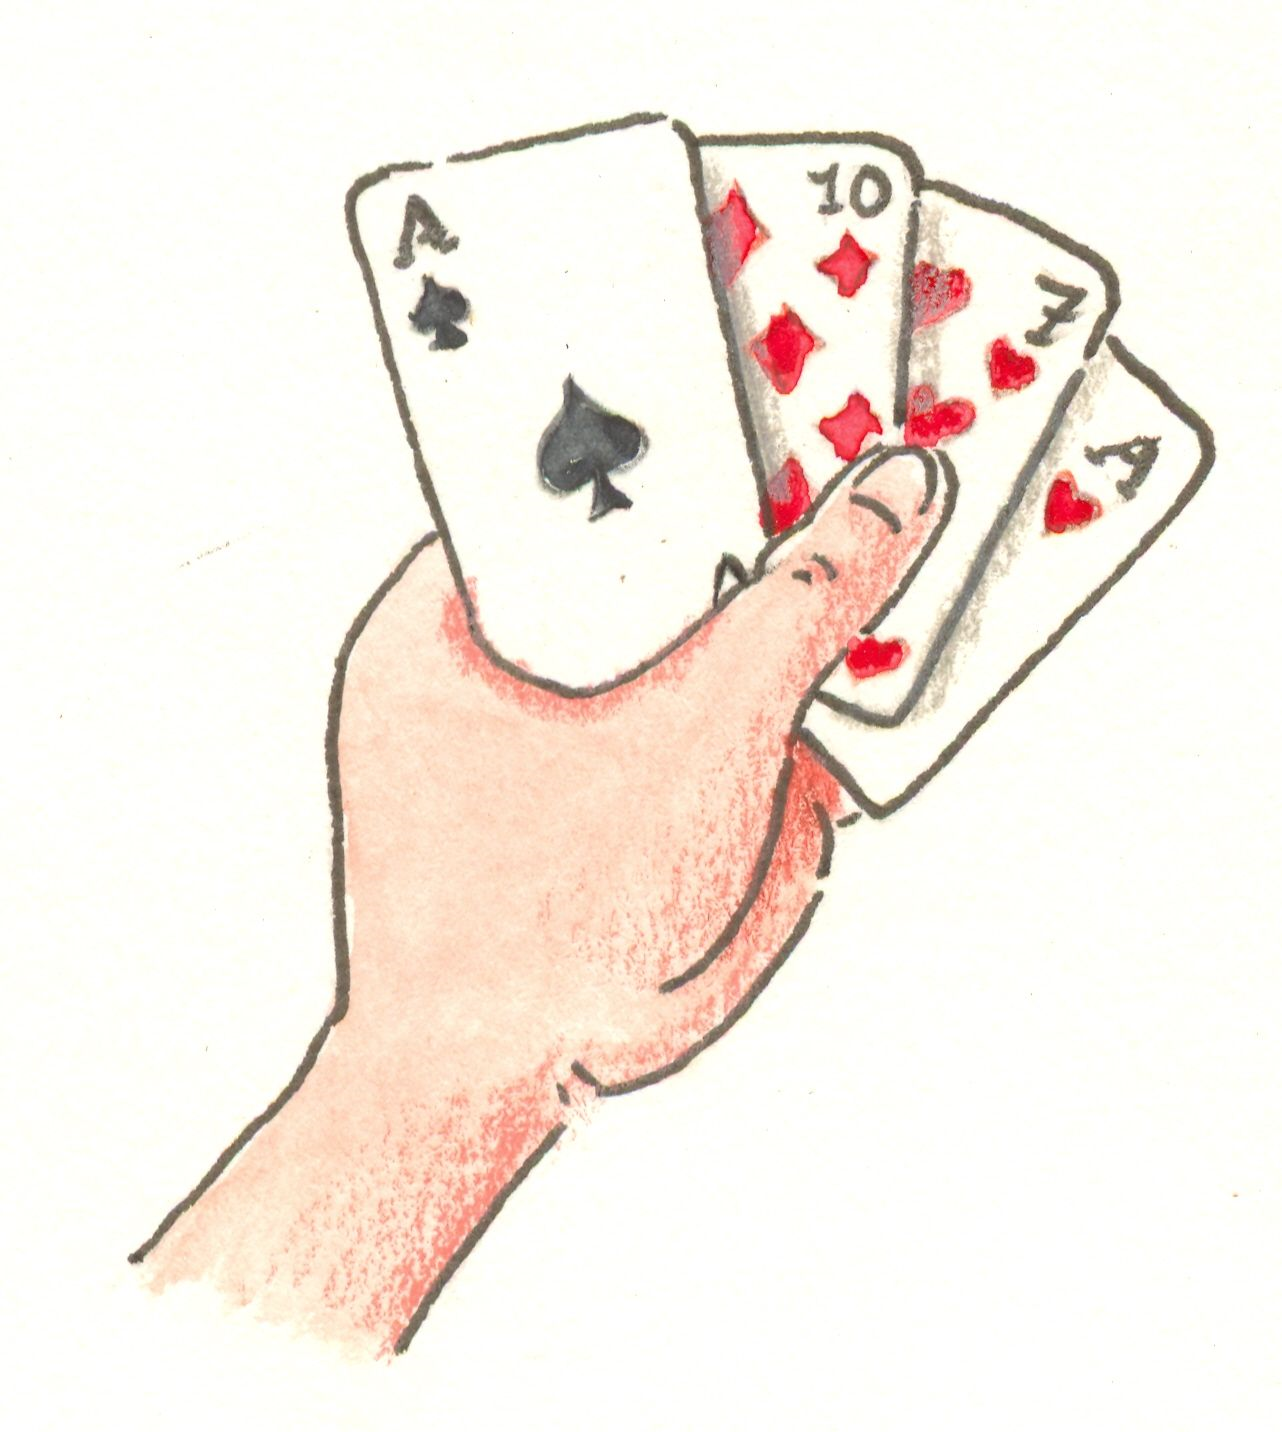
\includegraphics{kartenspiel}
\ \\
\ \\

\textbf{\textsc{\LARGE NET-WizHearts}}
\vspace{2cm}

\begin{tabular}{|c|c|c|}\hline
   Phase & Verantwortlicher & E-Mail \\ \hline\hline
   Pflichtenheft & Alina Meixl &  alina@meixl.de \\ \hline
   Entwurf & Viktoria Witka & witkaviktoria@freenet.de \\ \hline
   Spezifikation & Daniel Riedl & dariedl14@yahoo.de \\ \hline
   Implementation & Andreas Altenbuchner& a.andi007@gmail.com\\ \hline
   Verifikation & Patrick Kubin & kubin@fim.uni-passau.de\\ \hline
   Präsentation & w& w\\ \hline
 \end{tabular}
\end{center}
\end{titlepage}
\tableofcontents
\pagenumbering{arabic}
\hypersetup{pageanchor=true}

\section{Einleitung}
In diesem Dokument werden spezifische Angaben zu den bereits im Entwurf vorgestellten Klassen gemacht. Es werden im Folgenden Methoden und Attribute, sowie die Klassen genau beschrieben. Zunächst werden dazu die Änderungen vorgestellt, die seit dem Entwurf vorgenommen wurden. Des weiteren werden JUnit-Tests gezeigt, die zum Testen des späteren Programms essentiell sind. Zuletzt wird ein Implementierungsplan mit verschiedenen Milestones aufgezeigt. \\ \\

\section{Änderungen im Vergleich zum Entwurf}
\subsection{Server}
\subsubsection{Server}
Die Klasse Server war zuvor ein Interface und ist jetzt eine abstrakte Klasse von der der LobbyServer und der GameServer erben. So kann Codeduplikation vermieden werden.
\subsection{Client}
\subsubsection{Language}
Das Enum Language wurde in das Packet ClientView verschoben, da es von der View benötigt wird um die richtige Sprache anzuzeigen.
\subsubsection{MVMessage}
Die MVMessages wurden gelöscht und durch ein Enum ViewNotification ersetzt. Der Observer bekommt Änderungen über die Notifications mitgeteilt. Dies macht eine weitere Einteilung in einzelnde Messages unnötig.
\subsubsection{ClientState-Enum}
Dieses Enum enthält jeden Status, den ein Client erreichen kann.
\subsection{ClientView}
\subsubsection{MVMessages}
Dieses Interface wurde gelöscht, da es unnötig ist.
\subsubsection{ViewCard}
ViewCard ist die View-seitige Repräsentation einer Karte. Sie wird verwendet um einzelne Karten auf das Spielfeld zu zeichnen.
\subsection{Ruleset}
\subsubsection{ServerRuleset}
Das ServerRuleset ist statt einem Interface nun eine abstrakte Klasse, von der die Klassen ServerHearts (vorher Hearts) und ServerWizard (vorherWizard) erben. Codeduplikation kann so vermieden werden.
\subsubsection{ClientRuleset}
Das ClientRuleset ist statt einem Interface nun eine abstrakte Klasse, von der die Klassen ClientWizard und ClientHearts erben. So kann Codeduplikation vermieden werden.
\subsubsection{Card}
Die vorher abstrakte Klasse Card ist nun ein Interface, das von HeartsCard und WizardCard implementiert wird. So können die Methoden der Klasse Card von den anderen beiden so implementiert werden, wie es für das Spiel nötig ist.
\subsubsection{Colour}
Ein Enum Colour wurde hinzugefügt. Dieses enthält alle Farben, die eine Karte haben kann unabhängig vom Regelwerk.
\subsubsection{RulesetType}
Ein Enum RulesetType wurde hinzugefügt. Dieses enthält die Typen der Regelwerke, also deren Namen. 
\subsection{ComObjects}
\subsubsection{ComObject}
ComObject ist im Zuge des Einsetzens des VisitorPatterns von einer abstrakten Klassen zu einem Interface geändert worden.
\subsubsection{RulesetMessage}
RulesetMessage ist im Zuge des Einsetzens des VisitorPatterns von einer abstrakten Klassen zu einem Interface geändert worden.
\subsubsection{ComLogin}
Diese Klassen trägt den neuen Namen ComLoginRequest.
\subsubsection{ComKickPlayer}
Diese Klasse trägt den neuen Namen ComKickPlayerRequest.
\subsubsection{GameClientUpdate}
Diese Klasse wurde gelöscht, da sie unnötig ist.
\subsubsection{commands}
Dieses Enum wurde gelöscht, da es unnötig ist. An Stelle von diesem wurden weitere ComObjects hinzugefügt.
\subsubsection{types}
Dieses Enum wurde gelöscht, da es unnötig ist.
\subsubsection{ComBeenKicked}
Diese Klasse wurde zusätzlich hinzugefügt. Die Nachricht wird an einen Spieler gesendet, wenn er aus einem Spiel erntfernt wurde.
\subsubsection{ComClientLeave}
Diese Klasse wurde zusätzlich hinzugefügt. Sie wird zur Benachrichtigung gesendet, wenn ein Spieler ins nächste Fenster möchte und aus dem alten entfernt werden soll.
\subsubsection{ComClientQuit}
Diese Klasse wurde zusätzlich hinzugefügt. Die Nachricht wird verschickt, wenn der Spieler ein Fenster schließt.
\subsubsection{ComCreateGameRequest}
Diese Klasse wurde zusätzlich hinzugefügt. Diese Nachricht wird versendet, wenn ein neues Spiel erstellt werden soll.
\subsubsection{ComGameEnd}
Diese Klasse wurde zusätzlich hinzugefügt. Diese Nachricht wird versendet, wenn ein Spiel oder eine Runde zu Ende ist.
\subsubsection{ComServerAcknowledgement}
Diese Klasse wurde zusätzlich hinzugefügt. Diese Nachricht wird vom Server zur Bestätigung gesendet.
\subsubsection{ComStartGame}
Diese Klasse wurde zusätzlich hinzugefügt. Diese Nachricht wird versendet, wenn ein Spiel gestartet werden soll.
\subsubsection{ComWarning}
Diese Klasse wurde zusätzlich hinzugefügt. Diese Nachricht wird versendet, wenn ein Fehler passiert ist.
\subsubsection{MsgCardRequest}
Diese Klasse wurde zusätzlich hinzugefügt. Diese Nachricht wird von Server gesendet, um einem Spieler mitzuteilen, dass er das Spielen einer Karte erwartet.
\subsubsection{MsgMultiCardsRequest}
Diese Klasse wurde zusätzlich hinzugefügt.  Diese Nachricht wird gesendet, wenn die Auswahl mehrerer Karten vom Spieler gefordert werden soll.
\subsubsection{MsgNumberRequest}
Diese Klasse wurde zusätzlich hinzugefügt. Diese Nachricht wird gesendet, wenn die Eingabe einer Zahl gefordert werden soll.
\subsubsection{MsgSelectionRequest}
Diese Klasse wurde zusätzlich hinzugefügt. Diese Nachricht sendet der Server an einen Spieler, wenn er eine Farbauswahl von diesem erwartet.
\subsubsection{ComObjects-Klassen allgemein}
Da die ehemals abstrakten Klassen ComObject und RulesetMessage jetzt Interfaces sind, implementieren alle anderen Objekte diese statt von ihnen zu erben, des Weiteren implementieren alle Serializable.


%--- Begin generated contents ---
\section{Hierarchie-\/\-Verzeichnis}
\subsection{Klassenhierarchie}
Die Liste der Ableitungen ist -\/mit Einschränkungen-\/ alphabetisch sortiert\-:\begin{DoxyCompactList}
\item \contentsline{section}{Ruleset.\-Card}{\pageref{a00002}}{}
\begin{DoxyCompactList}
\item \contentsline{section}{Ruleset.\-Hearts\-Card}{\pageref{a00047}}{}
\item \contentsline{section}{Ruleset.\-Wizard\-Card}{\pageref{a00085}}{}
\end{DoxyCompactList}
\item \contentsline{section}{Ruleset.\-Card\-Deck}{\pageref{a00003}}{}
\item \contentsline{section}{Ruleset.\-Card\-Deck\-Builder}{\pageref{a00004}}{}
\item \contentsline{section}{Client.\-Card\-I\-D}{\pageref{a00005}}{}
\item \contentsline{section}{Client.\-Client\-Controller}{\pageref{a00008}}{}
\item \contentsline{section}{Client.\-Client\-Main}{\pageref{a00012}}{}
\item \contentsline{section}{Ruleset.\-Client\-Ruleset}{\pageref{a00014}}{}
\begin{DoxyCompactList}
\item \contentsline{section}{Ruleset.\-Client\-Hearts}{\pageref{a00009}}{}
\item \contentsline{section}{Ruleset.\-Client\-Wizard}{\pageref{a00016}}{}
\end{DoxyCompactList}
\item \contentsline{section}{Client.\-Client\-State}{\pageref{a00015}}{}
\item \contentsline{section}{Ruleset.\-Colour}{\pageref{a00017}}{}
\item \contentsline{section}{Com\-Objects.\-Com\-Been\-Kicked}{\pageref{a00018}}{}
\item \contentsline{section}{Client.\-View.\-Discard\-Pile}{\pageref{a00036}}{}
\item \contentsline{section}{Client.\-View.\-Draw\-Deck}{\pageref{a00037}}{}
\item \contentsline{section}{Ruleset.\-Game\-Client\-Update}{\pageref{a00039}}{}
\item \contentsline{section}{Ruleset.\-Game\-Phase}{\pageref{a00042}}{}
\item \contentsline{section}{Server.\-Game\-Server\-Representation}{\pageref{a00044}}{}
\item \contentsline{section}{Ruleset.\-Game\-State}{\pageref{a00045}}{}
\item \contentsline{section}{Ruleset.\-Hearths\-Deck}{\pageref{a00046}}{}
\item \contentsline{section}{Ruleset.\-Hearts\-I\-D}{\pageref{a00050}}{}
\item \contentsline{section}{Client.\-View.\-Language}{\pageref{a00052}}{}
\item \contentsline{section}{Client.\-Message\-Listener\-Thread}{\pageref{a00056}}{}
\item \contentsline{section}{Com\-Objects.\-Msg\-Card\-Request}{\pageref{a00058}}{}
\item \contentsline{section}{Client.\-M\-V\-Messages}{\pageref{a00068}}{}
\item \contentsline{section}{Ruleset.\-Other\-Data}{\pageref{a00069}}{}
\begin{DoxyCompactList}
\item \contentsline{section}{Ruleset.\-Hearts\-Data}{\pageref{a00049}}{}
\item \contentsline{section}{Ruleset.\-Wiz\-Data}{\pageref{a00088}}{}
\end{DoxyCompactList}
\item \contentsline{section}{Client.\-View.\-Other\-Player}{\pageref{a00070}}{}
\item \contentsline{section}{Client.\-View.\-Own\-Hand}{\pageref{a00071}}{}
\item \contentsline{section}{Ruleset.\-Player\-State}{\pageref{a00074}}{}
\item \contentsline{section}{Ruleset.\-Ruleset\-Type}{\pageref{a00076}}{}
\item Runnable\begin{DoxyCompactList}
\item \contentsline{section}{Server.\-Client\-Listener\-Thread}{\pageref{a00010}}{}
\item \contentsline{section}{Server.\-Lobby\-Server.\-Client\-Listener\-Thread}{\pageref{a00011}}{}
\item \contentsline{section}{Server.\-Player}{\pageref{a00073}}{}
\end{DoxyCompactList}
\item \contentsline{section}{Server.\-Server}{\pageref{a00078}}{}
\begin{DoxyCompactList}
\item \contentsline{section}{Server.\-Game\-Server}{\pageref{a00043}}{}
\item \contentsline{section}{Server.\-Lobby\-Server}{\pageref{a00054}}{}
\end{DoxyCompactList}
\item \contentsline{section}{Server.\-Server\-Main}{\pageref{a00080}}{}
\item \contentsline{section}{Ruleset.\-Server\-Ruleset}{\pageref{a00081}}{}
\begin{DoxyCompactList}
\item \contentsline{section}{Ruleset.\-Server\-Hearts}{\pageref{a00079}}{}
\item \contentsline{section}{Ruleset.\-Server\-Wizard}{\pageref{a00082}}{}
\end{DoxyCompactList}
\item \contentsline{section}{Client.\-View\-Notification}{\pageref{a00083}}{}
\item \contentsline{section}{Ruleset.\-Wizard\-Deck}{\pageref{a00086}}{}
\item \contentsline{section}{Ruleset.\-Wiz\-I\-D}{\pageref{a00089}}{}
\item J\-Frame\begin{DoxyCompactList}
\item \contentsline{section}{Client.\-View.\-Create\-Game}{\pageref{a00035}}{}
\item \contentsline{section}{Client.\-View.\-Game}{\pageref{a00038}}{}
\item \contentsline{section}{Client.\-View.\-Game\-Lobby}{\pageref{a00040}}{}
\item \contentsline{section}{Client.\-View.\-Lobby}{\pageref{a00053}}{}
\item \contentsline{section}{Client.\-View.\-Login}{\pageref{a00055}}{}
\item \contentsline{section}{Client.\-View.\-Password}{\pageref{a00072}}{}
\end{DoxyCompactList}
\item J\-Label\begin{DoxyCompactList}
\item \contentsline{section}{Client.\-View.\-Card}{\pageref{a00001}}{}
\begin{DoxyCompactList}
\item \contentsline{section}{Client.\-View.\-Hearts\-Card}{\pageref{a00048}}{}
\item \contentsline{section}{Client.\-View.\-Wiz\-Card}{\pageref{a00087}}{}
\end{DoxyCompactList}
\end{DoxyCompactList}
\item J\-Panel\begin{DoxyCompactList}
\item \contentsline{section}{Client.\-View.\-Game\-Panel}{\pageref{a00041}}{}
\end{DoxyCompactList}
\item Observable\begin{DoxyCompactList}
\item \contentsline{section}{Client.\-Client\-Model}{\pageref{a00013}}{}
\end{DoxyCompactList}
\item Observer\begin{DoxyCompactList}
\item \contentsline{section}{Client.\-View.\-Choose\-Cards}{\pageref{a00006}}{}
\item \contentsline{section}{Client.\-View.\-Choose\-Item}{\pageref{a00007}}{}
\item \contentsline{section}{Client.\-View.\-Create\-Game}{\pageref{a00035}}{}
\item \contentsline{section}{Client.\-View.\-Game}{\pageref{a00038}}{}
\item \contentsline{section}{Client.\-View.\-Game\-Lobby}{\pageref{a00040}}{}
\item \contentsline{section}{Client.\-View.\-Input\-Number}{\pageref{a00051}}{}
\item \contentsline{section}{Client.\-View.\-Lobby}{\pageref{a00053}}{}
\item \contentsline{section}{Client.\-View.\-Login}{\pageref{a00055}}{}
\item \contentsline{section}{Client.\-View.\-Password}{\pageref{a00072}}{}
\item \contentsline{section}{Client.\-View.\-Score\-Window}{\pageref{a00077}}{}
\item \contentsline{section}{Client.\-View.\-Warning}{\pageref{a00084}}{}
\end{DoxyCompactList}
\item Serializable\begin{DoxyCompactList}
\item \contentsline{section}{Com\-Objects.\-Com\-Object}{\pageref{a00029}}{}
\begin{DoxyCompactList}
\item \contentsline{section}{Com\-Objects.\-Com\-Chat\-Message}{\pageref{a00019}}{}
\item \contentsline{section}{Com\-Objects.\-Com\-Client\-Leave}{\pageref{a00020}}{}
\item \contentsline{section}{Com\-Objects.\-Com\-Client\-Quit}{\pageref{a00021}}{}
\item \contentsline{section}{Com\-Objects.\-Com\-Create\-Game\-Request}{\pageref{a00022}}{}
\item \contentsline{section}{Com\-Objects.\-Com\-Init\-Game\-Lobby}{\pageref{a00023}}{}
\item \contentsline{section}{Com\-Objects.\-Com\-Init\-Lobby}{\pageref{a00024}}{}
\item \contentsline{section}{Com\-Objects.\-Com\-Join\-Request}{\pageref{a00025}}{}
\item \contentsline{section}{Com\-Objects.\-Com\-Kick\-Player\-Request}{\pageref{a00026}}{}
\item \contentsline{section}{Com\-Objects.\-Com\-Lobby\-Update\-Gamelist}{\pageref{a00027}}{}
\item \contentsline{section}{Com\-Objects.\-Com\-Login\-Request}{\pageref{a00028}}{}
\item \contentsline{section}{Com\-Objects.\-Com\-Ruleset}{\pageref{a00030}}{}
\item \contentsline{section}{Com\-Objects.\-Com\-Server\-Acknowledgement}{\pageref{a00031}}{}
\item \contentsline{section}{Com\-Objects.\-Com\-Start\-Game}{\pageref{a00032}}{}
\item \contentsline{section}{Com\-Objects.\-Com\-Update\-Playerlist}{\pageref{a00033}}{}
\item \contentsline{section}{Com\-Objects.\-Com\-Warning}{\pageref{a00034}}{}
\end{DoxyCompactList}
\item \contentsline{section}{Com\-Objects.\-Ruleset\-Message}{\pageref{a00075}}{}
\begin{DoxyCompactList}
\item \contentsline{section}{Com\-Objects.\-Msg\-Card}{\pageref{a00057}}{}
\item \contentsline{section}{Com\-Objects.\-Msg\-Game\-End}{\pageref{a00059}}{}
\item \contentsline{section}{Com\-Objects.\-Msg\-Multi\-Cards}{\pageref{a00060}}{}
\item \contentsline{section}{Com\-Objects.\-Msg\-Multi\-Cards\-Request}{\pageref{a00061}}{}
\item \contentsline{section}{Com\-Objects.\-Msg\-Multiple\-Cards\-Request}{\pageref{a00062}}{}
\item \contentsline{section}{Com\-Objects.\-Msg\-Number}{\pageref{a00063}}{}
\item \contentsline{section}{Com\-Objects.\-Msg\-Number\-Request}{\pageref{a00064}}{}
\item \contentsline{section}{Com\-Objects.\-Msg\-Selection}{\pageref{a00065}}{}
\item \contentsline{section}{Com\-Objects.\-Msg\-Selection\-Request}{\pageref{a00066}}{}
\item \contentsline{section}{Com\-Objects.\-Msg\-User}{\pageref{a00067}}{}
\end{DoxyCompactList}
\end{DoxyCompactList}
\end{DoxyCompactList}

\section{Klassen-\/\-Verzeichnis}
\subsection{Auflistung der Klassen}
Hier folgt die Aufzählung aller Klassen, Strukturen, Varianten und Schnittstellen mit einer Kurzbeschreibung\-:\begin{DoxyCompactList}
\item\contentsline{section}{\hyperlink{a00001}{Client.\-View.\-Card} \\*\hyperlink{a00001}{Card} ist die View-\/seitige Repräsentation einer Karte }{\pageref{a00001}}{}
\item\contentsline{section}{\hyperlink{a00002}{Ruleset.\-Card} \\*Diese Klasse modelliert eine Spielkarte }{\pageref{a00002}}{}
\item\contentsline{section}{\hyperlink{a00003}{Ruleset.\-Card\-Deck} }{\pageref{a00003}}{}
\item\contentsline{section}{\hyperlink{a00004}{Ruleset.\-Card\-Deck\-Builder} }{\pageref{a00004}}{}
\item\contentsline{section}{\hyperlink{a00005}{Client.\-Card\-I\-D} }{\pageref{a00005}}{}
\item\contentsline{section}{\hyperlink{a00006}{Client.\-View.\-Choose\-Cards} }{\pageref{a00006}}{}
\item\contentsline{section}{\hyperlink{a00007}{Client.\-View.\-Choose\-Item} \\*Dieses Fenster ermöglicht es dem Spieler aus einer Liste von Items eines auszuwählen }{\pageref{a00007}}{}
\item\contentsline{section}{\hyperlink{a00008}{Client.\-Client\-Controller} }{\pageref{a00008}}{}
\item\contentsline{section}{\hyperlink{a00009}{Ruleset.\-Client\-Hearts} \\*Diese Klasse bildet das Regelwerk für den Client bei einer Partie Hearts }{\pageref{a00009}}{}
\item\contentsline{section}{\hyperlink{a00010}{Server.\-Client\-Listener\-Thread} }{\pageref{a00010}}{}
\item\contentsline{section}{\hyperlink{a00011}{Server.\-Lobby\-Server.\-Client\-Listener\-Thread} \\*Diese Klasse ist für das Zustandekommen von Clientverbindungen zuständig }{\pageref{a00011}}{}
\item\contentsline{section}{\hyperlink{a00012}{Client.\-Client\-Main} \\*Die \hyperlink{a00012}{Client\-Main} Klasse startet den Spielclient und initialisiert dessen Komponenten }{\pageref{a00012}}{}
\item\contentsline{section}{\hyperlink{a00013}{Client.\-Client\-Model} \\*Implementiert das Client Model }{\pageref{a00013}}{}
\item\contentsline{section}{\hyperlink{a00014}{Ruleset.\-Client\-Ruleset} \\*\hyperlink{a00014}{Client\-Ruleset} ist eine abstrakte Klasse und wird zur Regelvorauswertung im Client verwendet }{\pageref{a00014}}{}
\item\contentsline{section}{\hyperlink{a00015}{Client.\-Client\-State} \\*Dieser Enumerator enthält alle Zustände in denen sich der Client befinden kann }{\pageref{a00015}}{}
\item\contentsline{section}{\hyperlink{a00016}{Ruleset.\-Client\-Wizard} \\*Diese Klasse bildet das Regelwerk für den Client bei einer Partie Wizard }{\pageref{a00016}}{}
\item\contentsline{section}{\hyperlink{a00017}{Ruleset.\-Colour} \\*Repräsentiert die Farbe einer Karte }{\pageref{a00017}}{}
\item\contentsline{section}{\hyperlink{a00018}{Com\-Objects.\-Com\-Been\-Kicked} \\*Diese Klasse ist ein spezielles Kommunikations-\/\-Objekt }{\pageref{a00018}}{}
\item\contentsline{section}{\hyperlink{a00019}{Com\-Objects.\-Com\-Chat\-Message} \\*Diese Klasse ist ein spezielles Kommunikations-\/\-Objekt }{\pageref{a00019}}{}
\item\contentsline{section}{\hyperlink{a00020}{Com\-Objects.\-Com\-Client\-Leave} \\*Diese Klasse ist ein spezielles Kommunikations-\/\-Objekt }{\pageref{a00020}}{}
\item\contentsline{section}{\hyperlink{a00021}{Com\-Objects.\-Com\-Client\-Quit} \\*Diese Klasse ist ein spezielles Kommunikations-\/\-Objekt }{\pageref{a00021}}{}
\item\contentsline{section}{\hyperlink{a00022}{Com\-Objects.\-Com\-Create\-Game\-Request} \\*Diese Klasse ist ein spezielles Kommunikations-\/\-Objekt }{\pageref{a00022}}{}
\item\contentsline{section}{\hyperlink{a00023}{Com\-Objects.\-Com\-Init\-Game\-Lobby} \\*Diese Klasse ist ein spezielles Kommunikations-\/\-Objekt }{\pageref{a00023}}{}
\item\contentsline{section}{\hyperlink{a00024}{Com\-Objects.\-Com\-Init\-Lobby} \\*Diese Klasse ist ein spezielles Kommunikations-\/\-Objekt }{\pageref{a00024}}{}
\item\contentsline{section}{\hyperlink{a00025}{Com\-Objects.\-Com\-Join\-Request} \\*Diese Klasse ist ein spezielles Kommunikations-\/\-Objekt }{\pageref{a00025}}{}
\item\contentsline{section}{\hyperlink{a00026}{Com\-Objects.\-Com\-Kick\-Player\-Request} \\*Diese Klasse ist ein spezielles Kommunikations-\/\-Objekt }{\pageref{a00026}}{}
\item\contentsline{section}{\hyperlink{a00027}{Com\-Objects.\-Com\-Lobby\-Update\-Gamelist} \\*Diese Klasse ist ein spezielles Kommunikations-\/\-Objekt }{\pageref{a00027}}{}
\item\contentsline{section}{\hyperlink{a00028}{Com\-Objects.\-Com\-Login\-Request} \\*Diese Klasse ist ein spezielles Kommunikations-\/\-Objekt }{\pageref{a00028}}{}
\item\contentsline{section}{\hyperlink{a00029}{Com\-Objects.\-Com\-Object} }{\pageref{a00029}}{}
\item\contentsline{section}{\hyperlink{a00030}{Com\-Objects.\-Com\-Ruleset} \\*Diese Klasse ist ein spezielles Kommunikations-\/\-Objekt }{\pageref{a00030}}{}
\item\contentsline{section}{\hyperlink{a00031}{Com\-Objects.\-Com\-Server\-Acknowledgement} \\*Diese Klasse ist ein spezielles Kommunikations-\/\-Objekt }{\pageref{a00031}}{}
\item\contentsline{section}{\hyperlink{a00032}{Com\-Objects.\-Com\-Start\-Game} \\*Diese Klasse ist ein spezielles Kommunikations-\/\-Objekt }{\pageref{a00032}}{}
\item\contentsline{section}{\hyperlink{a00033}{Com\-Objects.\-Com\-Update\-Playerlist} \\*Diese Klasse ist ein spezielles Kommunikations-\/\-Objekt }{\pageref{a00033}}{}
\item\contentsline{section}{\hyperlink{a00034}{Com\-Objects.\-Com\-Warning} \\*Diese Klasse ist ein spezielles Kommunikations-\/\-Objekt }{\pageref{a00034}}{}
\item\contentsline{section}{\hyperlink{a00035}{Client.\-View.\-Create\-Game} \\*Das Fenster \hyperlink{a00035}{Create\-Game} dient dem Benutzer zur Erstellung eines neuen Spieles }{\pageref{a00035}}{}
\item\contentsline{section}{\hyperlink{a00036}{Client.\-View.\-Discard\-Pile} \\*Stellt einen Ablagestapel dar, dieser kann sowohl für jeden Spieler einzeln oder für alle Spieler gemeinsam in der Mitte des Spielfeldes angezeigt werden }{\pageref{a00036}}{}
\item\contentsline{section}{\hyperlink{a00037}{Client.\-View.\-Draw\-Deck} \\*Stellt einen Aufnahmestapel dar }{\pageref{a00037}}{}
\item\contentsline{section}{\hyperlink{a00038}{Client.\-View.\-Game} \\*Im \hyperlink{a00038}{Game} Fenster läuft das Spiel ab.\-Es enthält den Spielchat und ein \hyperlink{a00041}{Game\-Panel} }{\pageref{a00038}}{}
\item\contentsline{section}{\hyperlink{a00039}{Ruleset.\-Game\-Client\-Update} \\*Das \hyperlink{a00039}{Game\-Client\-Update} wird vom Rule\-Set aber den Game\-Server an den Client geschickt und enthalt alle Änderungen des \hyperlink{a00045}{Game\-State}, die für den Client relevant sind }{\pageref{a00039}}{}
\item\contentsline{section}{\hyperlink{a00040}{Client.\-View.\-Game\-Lobby} \\*Die \hyperlink{a00040}{Game\-Lobby} modelliert das Wartefenster, in dem beigetretene Spieler auf den Start des Spieles durch den Spielleiter warten }{\pageref{a00040}}{}
\item\contentsline{section}{\hyperlink{a00041}{Client.\-View.\-Game\-Panel} \\*Das Panel ist die Komponente des Game-\/\-Fensters, welche das eigentliche Spiel darstellt }{\pageref{a00041}}{}
\item\contentsline{section}{\hyperlink{a00042}{Ruleset.\-Game\-Phase} \\*Die \hyperlink{a00042}{Game\-Phase} modelliert die verschiedenen Zustände des Spiels im \hyperlink{a00045}{Game\-State} }{\pageref{a00042}}{}
\item\contentsline{section}{\hyperlink{a00043}{Server.\-Game\-Server} \\*Diese Klasse ist für die Spielverwaltung zuständig }{\pageref{a00043}}{}
\item\contentsline{section}{\hyperlink{a00044}{Server.\-Game\-Server\-Representation} \\*Dies eine Klasse, die Informationen über den Zustand eines Spielservers bereithält }{\pageref{a00044}}{}
\item\contentsline{section}{\hyperlink{a00045}{Ruleset.\-Game\-State} \\*Das \hyperlink{a00045}{Game\-State} modelliert einen aktuellen Spielzustand, es wird vom Game\-Server instanziert und vom Rule\-Set bearbeitet }{\pageref{a00045}}{}
\item\contentsline{section}{\hyperlink{a00046}{Ruleset.\-Hearths\-Deck} }{\pageref{a00046}}{}
\item\contentsline{section}{\hyperlink{a00047}{Ruleset.\-Hearts\-Card} \\*Modelliert eine Heartskarte }{\pageref{a00047}}{}
\item\contentsline{section}{\hyperlink{a00048}{Client.\-View.\-Hearts\-Card} \\*\hyperlink{a00048}{Hearts\-Card} ist die View-\/seitige Repräsentation einer Hearts-\/\-Karte }{\pageref{a00048}}{}
\item\contentsline{section}{\hyperlink{a00049}{Ruleset.\-Hearts\-Data} \\*Die zusätzlichen Informationen eines Spielers zum Spiel Hearts }{\pageref{a00049}}{}
\item\contentsline{section}{\hyperlink{a00050}{Ruleset.\-Hearts\-I\-D} \\*Die eindeutigen I\-Ds zu jeder Heartskarte }{\pageref{a00050}}{}
\item\contentsline{section}{\hyperlink{a00051}{Client.\-View.\-Input\-Number} \\*In diesem Fenster, kann der Benutzer eine Zahl eingeben }{\pageref{a00051}}{}
\item\contentsline{section}{\hyperlink{a00052}{Client.\-View.\-Language} \\*\hyperlink{a00052}{Language} stellt Repräsentationen verschiedener Sprachen dar, die von der G\-U\-I verwendet werden, um festzustellen welche Anzeigesprache verwendet werden soll }{\pageref{a00052}}{}
\item\contentsline{section}{\hyperlink{a00053}{Client.\-View.\-Lobby} \\*Diese Klasse erzeugt die Ansicht der Server\-Lobby auf der Client Seite, in der die Spieler neue Spiele erstellen oder offenen beitreten können }{\pageref{a00053}}{}
\item\contentsline{section}{\hyperlink{a00054}{Server.\-Lobby\-Server} \\*Diese Klasse ist für die Verwaltung der Spiellobby auf dem \hyperlink{a00078}{Server} verantwortlich }{\pageref{a00054}}{}
\item\contentsline{section}{\hyperlink{a00055}{Client.\-View.\-Login} \\*Das Login-\/\-Fenster repräsentiert den initialen Dialog zwischen Benutzer und Client }{\pageref{a00055}}{}
\item\contentsline{section}{\hyperlink{a00056}{Client.\-Message\-Listener\-Thread} }{\pageref{a00056}}{}
\item\contentsline{section}{\hyperlink{a00057}{Com\-Objects.\-Msg\-Card} \\*Diese Klasse ist eine Verfeinerung der Ruleset\-Message-\/\-Klasse }{\pageref{a00057}}{}
\item\contentsline{section}{\hyperlink{a00058}{Com\-Objects.\-Msg\-Card\-Request} \\*Diese Klasse ist eine Verfeinerung der Ruleset\-Message-\/\-Klasse }{\pageref{a00058}}{}
\item\contentsline{section}{\hyperlink{a00059}{Com\-Objects.\-Msg\-Game\-End} \\*Diese Klasse ist eine Verfeinerung der Ruleset\-Message-\/\-Klasse }{\pageref{a00059}}{}
\item\contentsline{section}{\hyperlink{a00060}{Com\-Objects.\-Msg\-Multi\-Cards} \\*Diese Klasse ist eine Verfeinerung der Ruleset\-Message-\/\-Klasse }{\pageref{a00060}}{}
\item\contentsline{section}{\hyperlink{a00061}{Com\-Objects.\-Msg\-Multi\-Cards\-Request} \\*Diese Klasse ist eine Verfeinerung der Ruleset\-Message-\/\-Klasse }{\pageref{a00061}}{}
\item\contentsline{section}{\hyperlink{a00062}{Com\-Objects.\-Msg\-Multiple\-Cards\-Request} \\*Diese Klasse ist eine Verfeinerung der Ruleset\-Message-\/\-Klasse }{\pageref{a00062}}{}
\item\contentsline{section}{\hyperlink{a00063}{Com\-Objects.\-Msg\-Number} \\*Diese Klasse ist eine Verfeinerung der Ruleset\-Message-\/\-Klasse }{\pageref{a00063}}{}
\item\contentsline{section}{\hyperlink{a00064}{Com\-Objects.\-Msg\-Number\-Request} \\*Diese Klasse ist eine Verfeinerung der Ruleset\-Message-\/\-Klasse }{\pageref{a00064}}{}
\item\contentsline{section}{\hyperlink{a00065}{Com\-Objects.\-Msg\-Selection} \\*Diese Klasse ist eine Verfeinerung der Ruleset\-Message-\/\-Klasse }{\pageref{a00065}}{}
\item\contentsline{section}{\hyperlink{a00066}{Com\-Objects.\-Msg\-Selection\-Request} \\*Diese Klasse ist eine Verfeinerung der Ruleset\-Message-\/\-Klasse }{\pageref{a00066}}{}
\item\contentsline{section}{\hyperlink{a00067}{Com\-Objects.\-Msg\-User} \\*Diese Klasse ist eine Verfeinerung der Ruleset\-Message-\/\-Klasse }{\pageref{a00067}}{}
\item\contentsline{section}{\hyperlink{a00068}{Client.\-M\-V\-Messages} }{\pageref{a00068}}{}
\item\contentsline{section}{\hyperlink{a00069}{Ruleset.\-Other\-Data} \\*\hyperlink{a00069}{Other\-Data} ist abstract und speichert die zusätzlichen Informationen eines Spielers }{\pageref{a00069}}{}
\item\contentsline{section}{\hyperlink{a00070}{Client.\-View.\-Other\-Player} \\*Zeigt die Informationen über die anderen Spieler an, also den Namen, ein Symbol für die verdeckte Hand und das Label für zusätzliche Angaben }{\pageref{a00070}}{}
\item\contentsline{section}{\hyperlink{a00071}{Client.\-View.\-Own\-Hand} \\*Stellt die Karten dar, die der Spieler auf der Hand hat }{\pageref{a00071}}{}
\item\contentsline{section}{\hyperlink{a00072}{Client.\-View.\-Password} \\*Dieses Fenster ermöglicht die Eingabe eines Passwortes um einem Passwortgeschütztem Spiel beizutreten oder per 'Leave' wieder in die \hyperlink{a00053}{Lobby} zurückzukehren }{\pageref{a00072}}{}
\item\contentsline{section}{\hyperlink{a00073}{Server.\-Player} \\*Die Player-\/\-Klasse wird zum Versenden von Java Serializable Objects verwendet }{\pageref{a00073}}{}
\item\contentsline{section}{\hyperlink{a00074}{Ruleset.\-Player\-State} \\*Repräsentiert den Spielzustand eines Spielers, und wird unter anderem im \hyperlink{a00045}{Game\-State} gespeichert }{\pageref{a00074}}{}
\item\contentsline{section}{\hyperlink{a00075}{Com\-Objects.\-Ruleset\-Message} \\*Diese Klasse ist eine Verfeinerung der Com\-Ruleset-\/\-Klasse }{\pageref{a00075}}{}
\item\contentsline{section}{\hyperlink{a00076}{Ruleset.\-Ruleset\-Type} \\*Die verschiedenen Regelwerke }{\pageref{a00076}}{}
\item\contentsline{section}{\hyperlink{a00077}{Client.\-View.\-Score\-Window} \\*Dieses Fenster zeigt den momentanen Punktestand nach jeder Runde und den Gesamtpunktestand am Ende des Spieles an }{\pageref{a00077}}{}
\item\contentsline{section}{\hyperlink{a00078}{Server.\-Server} \\*Ist ein abstrakte Klasse, von der die Klassen \hyperlink{a00054}{Lobby\-Server} und \hyperlink{a00043}{Game\-Server} erben }{\pageref{a00078}}{}
\item\contentsline{section}{\hyperlink{a00079}{Ruleset.\-Server\-Hearts} \\*Diese Klasse erstellt das Regelwerk zum Spiel Hearts }{\pageref{a00079}}{}
\item\contentsline{section}{\hyperlink{a00080}{Server.\-Server\-Main} \\*Diese Klasse startet den \hyperlink{a00078}{Server} und ist für die Konfigurationund Wartung des Servers verantwortlich }{\pageref{a00080}}{}
\item\contentsline{section}{\hyperlink{a00081}{Ruleset.\-Server\-Ruleset} \\*Das \hyperlink{a00081}{Server\-Ruleset} ist eine akstrakte Klasse und für den Ablauf und die Einhaltung der Regeln eines Spiels zuständig (/\-L280/) }{\pageref{a00081}}{}
\item\contentsline{section}{\hyperlink{a00082}{Ruleset.\-Server\-Wizard} \\*Diese Klasse erstellt das Regelwerk zum Spiel Wizard }{\pageref{a00082}}{}
\item\contentsline{section}{\hyperlink{a00083}{Client.\-View\-Notification} }{\pageref{a00083}}{}
\item\contentsline{section}{\hyperlink{a00084}{Client.\-View.\-Warning} \\*Das Warning-\/\-Fenster zeigt dem Benutzer Fehlermeldungen bzw }{\pageref{a00084}}{}
\item\contentsline{section}{\hyperlink{a00085}{Ruleset.\-Wizard\-Card} \\*Modelliert eine Wizardkarte }{\pageref{a00085}}{}
\item\contentsline{section}{\hyperlink{a00086}{Ruleset.\-Wizard\-Deck} }{\pageref{a00086}}{}
\item\contentsline{section}{\hyperlink{a00087}{Client.\-View.\-Wiz\-Card} \\*\hyperlink{a00087}{Wiz\-Card} ist die View-\/seitige Repräsentation einer Wizard-\/\-Karte }{\pageref{a00087}}{}
\item\contentsline{section}{\hyperlink{a00088}{Ruleset.\-Wiz\-Data} \\*Die zusätzlichen Informationen eines Spielers zum Spiel Wizard }{\pageref{a00088}}{}
\item\contentsline{section}{\hyperlink{a00089}{Ruleset.\-Wiz\-I\-D} \\*Die eindeutigen I\-Ds zu jeder Wizardkarte }{\pageref{a00089}}{}
\end{DoxyCompactList}

\section{Klassen-\/\-Dokumentation}
\hypertarget{a00001}{\subsection{Client.\-View.\-Card Klassenreferenz}
\label{a00001}\index{Client.\-View.\-Card@{Client.\-View.\-Card}}
}
Klassendiagramm für Client.\-View.\-Card\-:\begin{figure}[H]
\begin{center}
\leavevmode
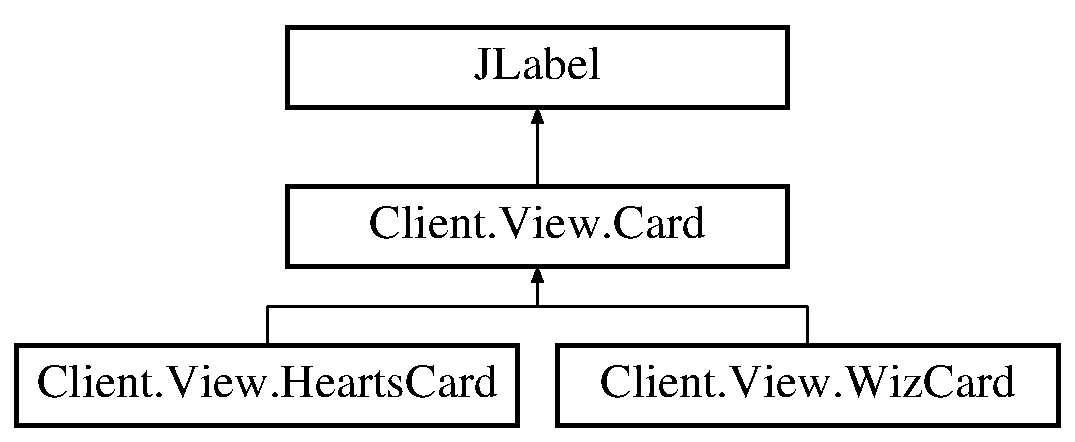
\includegraphics[height=3.000000cm]{a00001}
\end{center}
\end{figure}
\subsubsection*{Öffentliche Methoden}
\begin{DoxyCompactItemize}
\item 
\hyperlink{a00001_a97eccc3cbe788dd025fe0b8e75165181}{Card} (String s)
\end{DoxyCompactItemize}


\subsubsection{Ausführliche Beschreibung}
Sie wird verwendet um einzelne Karten auf das Spielfeld zu zeichnen. Dazu enthält sie die Pfadangabe zu dem Ordner, in dem die Bilder der Karten gespeichert sind, und eine I\-D, um das genaue Bild zu spezifizieren. 

\subsubsection{Beschreibung der Konstruktoren und Destruktoren}
\hypertarget{a00001_a97eccc3cbe788dd025fe0b8e75165181}{\index{Client\-::\-View\-::\-Card@{Client\-::\-View\-::\-Card}!Card@{Card}}
\index{Card@{Card}!Client::View::Card@{Client\-::\-View\-::\-Card}}
\paragraph[{Card}]{\setlength{\rightskip}{0pt plus 5cm}Client.\-View.\-Card.\-Card (
\begin{DoxyParamCaption}
\item[{String}]{s}
\end{DoxyParamCaption}
)}}\label{a00001_a97eccc3cbe788dd025fe0b8e75165181}


Erstellt eine neue Karte für die Anzeige und zeichnet dafür das Bild, das durch die Pfadangabe s angegeben ist. 


\begin{DoxyParams}{Parameter}
{\em s} & Pfadangabe zum zu zeichnenden Bild \\
\hline
\end{DoxyParams}

\hypertarget{a00002}{\subsection{Client\-Main Klassenreferenz}
\label{a00002}\index{Client\-Main@{Client\-Main}}
}
\subsubsection*{Öffentliche, statische Methoden}
\begin{DoxyCompactItemize}
\item 
static void \hyperlink{a00002_afd8ce3c47844bcb10ccd52d43dc4d339}{main} (final String\mbox{[}$\,$\mbox{]} args)
\end{DoxyCompactItemize}
\subsubsection*{Private Attribute}
\begin{DoxyCompactItemize}
\item 
\hypertarget{a00002_acb404ab350ff7496df1d66c7c638a7bd}{\hyperlink{a00001}{Client\-Controller} \hyperlink{a00002_acb404ab350ff7496df1d66c7c638a7bd}{client\-Controller}}\label{a00002_acb404ab350ff7496df1d66c7c638a7bd}

\end{DoxyCompactItemize}


\subsubsection{Ausführliche Beschreibung}
Die \hyperlink{a00002}{Client\-Main} Klasse startet den Spielclient und initialisiert dessen Komponenten. 

\subsubsection{Dokumentation der Elementfunktionen}
\hypertarget{a00002_afd8ce3c47844bcb10ccd52d43dc4d339}{\index{Client\-::\-Client\-Main@{Client\-::\-Client\-Main}!main@{main}}
\index{main@{main}!Client::ClientMain@{Client\-::\-Client\-Main}}
\paragraph[{main}]{\setlength{\rightskip}{0pt plus 5cm}static void main (
\begin{DoxyParamCaption}
\item[{final String\mbox{[}$\,$\mbox{]}}]{args}
\end{DoxyParamCaption}
)\hspace{0.3cm}{\ttfamily [static]}}}\label{a00002_afd8ce3c47844bcb10ccd52d43dc4d339}

\begin{DoxyParams}{Parameter}
{\em args} & \\
\hline
\end{DoxyParams}

\hypertarget{a00003}{\subsection{Ruleset.\-Card\-Deck Klassenreferenz}
\label{a00003}\index{Ruleset.\-Card\-Deck@{Ruleset.\-Card\-Deck}}
}

\hypertarget{a00004}{\subsection{Ruleset.\-Client\-Wizard Klassenreferenz}
\label{a00004}\index{Ruleset.\-Client\-Wizard@{Ruleset.\-Client\-Wizard}}
}
Klassendiagramm für Ruleset.\-Client\-Wizard\-:\begin{figure}[H]
\begin{center}
\leavevmode
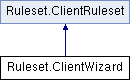
\includegraphics[height=2.000000cm]{a00004}
\end{center}
\end{figure}
\subsubsection*{Öffentliche Methoden}
\begin{DoxyCompactItemize}
\item 
boolean \hyperlink{a00004_a375a6aca8ba78551d0da0f6840cec6aa}{is\-Valid\-Move} (\hyperlink{a00001}{Card} card)
\end{DoxyCompactItemize}


\subsubsection{Ausführliche Beschreibung}
\begin{DoxyAuthor}{Autor}
m4nkey  \char`\"{}\-U\-M\-L to Java (com.\-ibm.\-xtools.\-transform.\-uml2.\-java5.\-internal.\-U\-M\-L2\-Java\-Transform)\char`\"{} 
\end{DoxyAuthor}


\subsubsection{Dokumentation der Elementfunktionen}
\hypertarget{a00004_a375a6aca8ba78551d0da0f6840cec6aa}{\index{Ruleset\-::\-Client\-Wizard@{Ruleset\-::\-Client\-Wizard}!is\-Valid\-Move@{is\-Valid\-Move}}
\index{is\-Valid\-Move@{is\-Valid\-Move}!Ruleset::ClientWizard@{Ruleset\-::\-Client\-Wizard}}
\paragraph[{is\-Valid\-Move}]{\setlength{\rightskip}{0pt plus 5cm}boolean Ruleset.\-Client\-Wizard.\-is\-Valid\-Move (
\begin{DoxyParamCaption}
\item[{{\bf Card}}]{card}
\end{DoxyParamCaption}
)\hspace{0.3cm}{\ttfamily [virtual]}}}\label{a00004_a375a6aca8ba78551d0da0f6840cec6aa}


Pr�ft ob ein gemachter Zug zum Spiel Wizard g�ltig ist. 

\begin{DoxyReturn}{Rückgabe}
is\-Valid true falls Zug g�ltig, false wenn nicht 
\end{DoxyReturn}


Implementiert \hyperlink{a00003_aa335aa62f13ac6ef532aef65a8cb34c0}{Ruleset.\-Client\-Ruleset}.


\hypertarget{a00005}{\subsection{Message\-Listener\-Thread Klassenreferenz}
\label{a00005}\index{Message\-Listener\-Thread@{Message\-Listener\-Thread}}
}


Abgeleitet von Thread.

\subsubsection*{Öffentliche Methoden}
\begin{DoxyCompactItemize}
\item 
\hypertarget{a00005_a90ebca0a8a2d843065708a4473f4428d}{\hyperlink{a00005_a90ebca0a8a2d843065708a4473f4428d}{Message\-Listener\-Thread} ()}\label{a00005_a90ebca0a8a2d843065708a4473f4428d}

\item 
void \hyperlink{a00005_a9b5e6f31c533ba11eada7bdd1767bf10}{start\-Connection} (\hyperlink{a00003}{Client\-Model} model, Socket connection)  throws Illegal\-Argument\-Exception, I\-O\-Exception 
\item 
\hypertarget{a00005_aaf912c696192e6a13eb70526891b4cd2}{void \hyperlink{a00005_aaf912c696192e6a13eb70526891b4cd2}{close\-Connection} ()}\label{a00005_aaf912c696192e6a13eb70526891b4cd2}

\item 
\hypertarget{a00005_afea035a8450d55661a10d4727154498d}{void \hyperlink{a00005_afea035a8450d55661a10d4727154498d}{send} (\hyperlink{a00037}{Com\-Object} object)}\label{a00005_afea035a8450d55661a10d4727154498d}

\item 
\hypertarget{a00005_a13a43e6d814de94978c515cb084873b1}{void \hyperlink{a00005_a13a43e6d814de94978c515cb084873b1}{run} ()}\label{a00005_a13a43e6d814de94978c515cb084873b1}

\end{DoxyCompactItemize}
\subsubsection*{Private Attribute}
\begin{DoxyCompactItemize}
\item 
\hypertarget{a00005_a5ea451c5997894ff409c7feb3ed28448}{Socket {\bfseries socket}}\label{a00005_a5ea451c5997894ff409c7feb3ed28448}

\item 
\hypertarget{a00005_af04a77f17fee54627c647f7d430fd7e4}{Object\-Input {\bfseries in}}\label{a00005_af04a77f17fee54627c647f7d430fd7e4}

\item 
\hypertarget{a00005_aaa47df5af3623385a32344b55b1aa173}{Object\-Output {\bfseries out}}\label{a00005_aaa47df5af3623385a32344b55b1aa173}

\item 
\hypertarget{a00005_acd2be1cfc258f9da5c30cf341d2a8804}{boolean {\bfseries run} = false}\label{a00005_acd2be1cfc258f9da5c30cf341d2a8804}

\item 
\hypertarget{a00005_a816de8cbcf19fd6762e3c5e5c66af478}{\hyperlink{a00003}{Client\-Model} {\bfseries model}}\label{a00005_a816de8cbcf19fd6762e3c5e5c66af478}

\end{DoxyCompactItemize}


\subsubsection{Ausführliche Beschreibung}
Diese Klasse implementiert die Netzwerkanbindung des Clients an den Server. Sie enthaelt den dazu noetigen Socket und Objekt\-Stream Reader und Writer. 

\subsubsection{Dokumentation der Elementfunktionen}
\hypertarget{a00005_a9b5e6f31c533ba11eada7bdd1767bf10}{\index{Client\-::\-Message\-Listener\-Thread@{Client\-::\-Message\-Listener\-Thread}!start\-Connection@{start\-Connection}}
\index{start\-Connection@{start\-Connection}!Client::MessageListenerThread@{Client\-::\-Message\-Listener\-Thread}}
\paragraph[{start\-Connection}]{\setlength{\rightskip}{0pt plus 5cm}void start\-Connection (
\begin{DoxyParamCaption}
\item[{{\bf Client\-Model}}]{model, }
\item[{Socket}]{connection}
\end{DoxyParamCaption}
) throws Illegal\-Argument\-Exception, I\-O\-Exception}}\label{a00005_a9b5e6f31c533ba11eada7bdd1767bf10}


Initialisiert die Object\-Streams und speichert den T\-C\-P Socket im Thread. 


\begin{DoxyParams}{Parameter}
{\em model} & \hyperlink{a00003}{Client\-Model}, Das Model das den Spielablauf und Serverkommunikation steuert. \\
\hline
{\em connection} & Socket, der Socket über den die T\-C\-P Verbindung laeuft. \\
\hline
\end{DoxyParams}

\begin{DoxyExceptions}{Ausnahmebehandlung}
{\em Illegal\-Argument\-Exception} & Wird geworfen bei falschen \hyperlink{a00003}{Client\-Model} oder Socket Argumenten. \\
\hline
{\em I\-O\-Exception} & Wird geworfen beim fehlerbehafteten Erstellen der Object\-Streams. \\
\hline
\end{DoxyExceptions}

\hypertarget{a00006}{\subsection{Choose\-Cards Klassenreferenz}
\label{a00006}\index{Choose\-Cards@{Choose\-Cards}}
}


Abgeleitet von Observer.

\subsubsection*{Öffentliche Methoden}
\begin{DoxyCompactItemize}
\item 
void \hyperlink{a00006_a2b67d42550fdf9ddd8f3878d0849965c}{update} (Observable o, Object arg)
\end{DoxyCompactItemize}
\subsubsection*{Private Attribute}
\begin{DoxyCompactItemize}
\item 
\hypertarget{a00006_a78a1f793ce7650a7cfefc4a7e4d14a04}{\hyperlink{a00019}{Own\-Hand} {\bfseries player\-Hand\-Panel}}\label{a00006_a78a1f793ce7650a7cfefc4a7e4d14a04}

\end{DoxyCompactItemize}


\subsubsection{Ausführliche Beschreibung}
In diesem Fenster muss der Benutzer eine vorbestimmte Menge Karten auswaehlen. 

\subsubsection{Dokumentation der Elementfunktionen}
\hypertarget{a00006_a2b67d42550fdf9ddd8f3878d0849965c}{\index{Client\-::\-View\-::\-Choose\-Cards@{Client\-::\-View\-::\-Choose\-Cards}!update@{update}}
\index{update@{update}!Client::View::ChooseCards@{Client\-::\-View\-::\-Choose\-Cards}}
\paragraph[{update}]{\setlength{\rightskip}{0pt plus 5cm}void update (
\begin{DoxyParamCaption}
\item[{Observable}]{o, }
\item[{Object}]{arg}
\end{DoxyParamCaption}
)}}\label{a00006_a2b67d42550fdf9ddd8f3878d0849965c}


Wird durch notify() im \hyperlink{a00003}{Client\-Model} aufgerufen. 

Je nach dem in arg uebergebenen Befehl wird ein Update des Fensters ausgefuehrt oder eine Fehlermeldung angezeigt.


\begin{DoxyParams}{Parameter}
{\em o} & erwartet ein Objekt von der Klasse \hyperlink{a00003}{Client\-Model} \\
\hline
{\em arg} & erwartet\-: open\-Choose\-Cards, choose\-Cards\-Successful \\
\hline
\end{DoxyParams}

\hypertarget{a00007}{\subsection{Choose\-Item Klassenreferenz}
\label{a00007}\index{Choose\-Item@{Choose\-Item}}
}


Abgeleitet von Observer.

\subsubsection*{Öffentliche Methoden}
\begin{DoxyCompactItemize}
\item 
void \hyperlink{a00007_a5e5bb525779faa05530c9ebdc49ad123}{update} (Observable arg0, Object arg1)
\end{DoxyCompactItemize}
\subsubsection*{Private Attribute}
\begin{DoxyCompactItemize}
\item 
\hypertarget{a00007_a5eae36bb5790864ced94623c9d08cb90}{Object {\bfseries item\-Combo\-Box}}\label{a00007_a5eae36bb5790864ced94623c9d08cb90}

\end{DoxyCompactItemize}


\subsubsection{Ausführliche Beschreibung}
Dieses Fenster ermoeglicht es dem Spieler aus einer Liste von Items eines auszuwaehlen. 

\subsubsection{Dokumentation der Elementfunktionen}
\hypertarget{a00007_a5e5bb525779faa05530c9ebdc49ad123}{\index{Client\-::\-View\-::\-Choose\-Item@{Client\-::\-View\-::\-Choose\-Item}!update@{update}}
\index{update@{update}!Client::View::ChooseItem@{Client\-::\-View\-::\-Choose\-Item}}
\paragraph[{update}]{\setlength{\rightskip}{0pt plus 5cm}void update (
\begin{DoxyParamCaption}
\item[{Observable}]{arg0, }
\item[{Object}]{arg1}
\end{DoxyParamCaption}
)}}\label{a00007_a5e5bb525779faa05530c9ebdc49ad123}


Wird durch notify() im \hyperlink{a00003}{Client\-Model} aufgerufen. 

Je nach dem in arg uebergebenen Befehl wird ein Update des Fensters ausgefuehrt oder eine Fehlermeldung angezeigt.


\begin{DoxyParams}{Parameter}
{\em o} & erwartet ein Objekt von der Klasse \hyperlink{a00003}{Client\-Model} \\
\hline
{\em arg} & erwartet\-: open\-Choose\-Item, choose\-Item\-Successful \\
\hline
\end{DoxyParams}

\hypertarget{a00008}{\subsection{Create\-Game Klassenreferenz}
\label{a00008}\index{Create\-Game@{Create\-Game}}
}


Abgeleitet von J\-Frame.

\subsubsection*{Öffentliche Methoden}
\begin{DoxyCompactItemize}
\item 
\hypertarget{a00008_a9c81ed380a56f523fd8a7b0c8fc349f7}{\hyperlink{a00008_a9c81ed380a56f523fd8a7b0c8fc349f7}{Create\-Game} ()}\label{a00008_a9c81ed380a56f523fd8a7b0c8fc349f7}

\item 
void \hyperlink{a00008_a0e4f14000bb92efe86644965867a5156}{add\-Panel\-Mouse\-Listener} (Mouse\-Listener m)
\item 
void \hyperlink{a00008_acf3b22c2ad67e52fbd300665503a0cb5}{add\-Ruleset\-Selection\-Listener} (Item\-Listener i)
\item 
void \hyperlink{a00008_a766141ddea860fac0deb3ceb1c65ed60}{add\-Create\-Button\-Listener} (Action\-Listener a)
\item 
void \hyperlink{a00008_aac8c97a2425ab3702a82bb0876aa3cc8}{add\-Leave\-Button\-Listener} (Action\-Listener a)
\item 
void \hyperlink{a00008_a9329ba7453dd661d50d2fb8024df3b2b}{set\-Language} (\hyperlink{a00015}{Language} l)
\end{DoxyCompactItemize}
\subsubsection*{Öffentliche, statische Methoden}
\begin{DoxyCompactItemize}
\item 
\hypertarget{a00008_a8b260eecbaabcef8473fd87ada040682}{static void {\bfseries main} (String\mbox{[}$\,$\mbox{]} args)}\label{a00008_a8b260eecbaabcef8473fd87ada040682}

\end{DoxyCompactItemize}
\subsubsection*{Private Methoden}
\begin{DoxyCompactItemize}
\item 
\hypertarget{a00008_a74cba330cee84fa07487e12fdafe29aa}{void {\bfseries update\-Language} ()}\label{a00008_a74cba330cee84fa07487e12fdafe29aa}

\end{DoxyCompactItemize}
\subsubsection*{Private Attribute}
\begin{DoxyCompactItemize}
\item 
\hypertarget{a00008_a430764470b3602491655161cdd67ee8c}{\hyperlink{a00015}{Language} {\bfseries lang}}\label{a00008_a430764470b3602491655161cdd67ee8c}

\item 
\hypertarget{a00008_a2b4470f7f3f7456c7e52d1604438a878}{J\-Text\-Field {\bfseries name\-Field}}\label{a00008_a2b4470f7f3f7456c7e52d1604438a878}

\item 
\hypertarget{a00008_a45e94f786577439d02e4f16aefa96717}{Buffered\-Image {\bfseries image}}\label{a00008_a45e94f786577439d02e4f16aefa96717}

\item 
\hypertarget{a00008_ab86817c3677c2dc422445fe8c0b5a404}{J\-Text\-Field {\bfseries password\-Field}}\label{a00008_ab86817c3677c2dc422445fe8c0b5a404}

\item 
\hypertarget{a00008_a8f4aaa528d2092952844a99aa948932f}{J\-Panel {\bfseries image\-Panel}}\label{a00008_a8f4aaa528d2092952844a99aa948932f}

\item 
\hypertarget{a00008_ac3a56e854d86f838fbfe3bad5fca49ea}{J\-Label {\bfseries lbl\-Select}}\label{a00008_ac3a56e854d86f838fbfe3bad5fca49ea}

\item 
\hypertarget{a00008_a7916a564649b0412714b6ea8c2251812}{J\-Combo\-Box$<$ String $>$ {\bfseries ruleset\-Box}}\label{a00008_a7916a564649b0412714b6ea8c2251812}

\item 
\hypertarget{a00008_a5df88a40b8ff9b13b83ca12563ba89c7}{J\-Check\-Box {\bfseries chckbx\-Password}}\label{a00008_a5df88a40b8ff9b13b83ca12563ba89c7}

\item 
\hypertarget{a00008_a1887f14b78aa91b00e5ce42aa504dbe2}{J\-Button {\bfseries btn\-Leave}}\label{a00008_a1887f14b78aa91b00e5ce42aa504dbe2}

\item 
\hypertarget{a00008_a69446706c0a5c7165a4de4f64d7b2261}{J\-Button {\bfseries btn\-Create}}\label{a00008_a69446706c0a5c7165a4de4f64d7b2261}

\item 
\hypertarget{a00008_a59c71155f1fd33a521bce1afebc0863b}{J\-Label {\bfseries lbl\-Game\-Name}}\label{a00008_a59c71155f1fd33a521bce1afebc0863b}

\end{DoxyCompactItemize}
\subsubsection*{Statische, private Attribute}
\begin{DoxyCompactItemize}
\item 
\hypertarget{a00008_a3238d314ecdee14d2966760945d00c3b}{static final long {\bfseries serial\-Version\-U\-I\-D} = -\/2893031560688870723\-L}\label{a00008_a3238d314ecdee14d2966760945d00c3b}

\end{DoxyCompactItemize}


\subsubsection{Ausführliche Beschreibung}
Das Fenster \hyperlink{a00008}{Create\-Game} dient dem Benutzer zur Erstellung eines neuen Spieles. Es bietet alle Komponenten, um ein Regelwerk zu waehlen, einen Spielnamen festzulegen und das Spiel durch ein Passwort zu schuetzen. In der Spielerstellung wird ein Titelbild des ausgewaehlten Spiels und eine kurze Beschreibung angezeigt. ueber 'Leave' kehrt der Spieler in die \hyperlink{a00016}{Lobby} zurueck und mit 'Create' wird das Spiel erstellt. 

\subsubsection{Dokumentation der Elementfunktionen}
\hypertarget{a00008_a0e4f14000bb92efe86644965867a5156}{\index{Client\-::\-View\-::\-Create\-Game@{Client\-::\-View\-::\-Create\-Game}!add\-Panel\-Mouse\-Listener@{add\-Panel\-Mouse\-Listener}}
\index{add\-Panel\-Mouse\-Listener@{add\-Panel\-Mouse\-Listener}!Client::View::CreateGame@{Client\-::\-View\-::\-Create\-Game}}
\paragraph[{add\-Panel\-Mouse\-Listener}]{\setlength{\rightskip}{0pt plus 5cm}void add\-Panel\-Mouse\-Listener (
\begin{DoxyParamCaption}
\item[{Mouse\-Listener}]{m}
\end{DoxyParamCaption}
)}}\label{a00008_a0e4f14000bb92efe86644965867a5156}


Fuegt einen Mouse\-Listener zum Image\-Panel des \hyperlink{a00008}{Create\-Game} Fensters hinzu, der zur Anzeige des Mouse\-Over-\/\-Texts verwendet wird. 


\begin{DoxyParams}{Parameter}
{\em m} & ein Mouse\-Listener \\
\hline
\end{DoxyParams}
\hypertarget{a00008_acf3b22c2ad67e52fbd300665503a0cb5}{\index{Client\-::\-View\-::\-Create\-Game@{Client\-::\-View\-::\-Create\-Game}!add\-Ruleset\-Selection\-Listener@{add\-Ruleset\-Selection\-Listener}}
\index{add\-Ruleset\-Selection\-Listener@{add\-Ruleset\-Selection\-Listener}!Client::View::CreateGame@{Client\-::\-View\-::\-Create\-Game}}
\paragraph[{add\-Ruleset\-Selection\-Listener}]{\setlength{\rightskip}{0pt plus 5cm}void add\-Ruleset\-Selection\-Listener (
\begin{DoxyParamCaption}
\item[{Item\-Listener}]{i}
\end{DoxyParamCaption}
)}}\label{a00008_acf3b22c2ad67e52fbd300665503a0cb5}


Fuegt einen Listener fuer die Regelwerk-\/\-Auswahl des \hyperlink{a00008}{Create\-Game} Fensters hinzu. 


\begin{DoxyParams}{Parameter}
{\em i} & ein Item\-Listener \\
\hline
\end{DoxyParams}
\hypertarget{a00008_a766141ddea860fac0deb3ceb1c65ed60}{\index{Client\-::\-View\-::\-Create\-Game@{Client\-::\-View\-::\-Create\-Game}!add\-Create\-Button\-Listener@{add\-Create\-Button\-Listener}}
\index{add\-Create\-Button\-Listener@{add\-Create\-Button\-Listener}!Client::View::CreateGame@{Client\-::\-View\-::\-Create\-Game}}
\paragraph[{add\-Create\-Button\-Listener}]{\setlength{\rightskip}{0pt plus 5cm}void add\-Create\-Button\-Listener (
\begin{DoxyParamCaption}
\item[{Action\-Listener}]{a}
\end{DoxyParamCaption}
)}}\label{a00008_a766141ddea860fac0deb3ceb1c65ed60}


Fuegt einen Action\-Listener fuer den 'Create' Button hinzu. 


\begin{DoxyParams}{Parameter}
{\em a} & ein Action\-Listener \\
\hline
\end{DoxyParams}
\hypertarget{a00008_aac8c97a2425ab3702a82bb0876aa3cc8}{\index{Client\-::\-View\-::\-Create\-Game@{Client\-::\-View\-::\-Create\-Game}!add\-Leave\-Button\-Listener@{add\-Leave\-Button\-Listener}}
\index{add\-Leave\-Button\-Listener@{add\-Leave\-Button\-Listener}!Client::View::CreateGame@{Client\-::\-View\-::\-Create\-Game}}
\paragraph[{add\-Leave\-Button\-Listener}]{\setlength{\rightskip}{0pt plus 5cm}void add\-Leave\-Button\-Listener (
\begin{DoxyParamCaption}
\item[{Action\-Listener}]{a}
\end{DoxyParamCaption}
)}}\label{a00008_aac8c97a2425ab3702a82bb0876aa3cc8}


Fuegt einen Action\-Listener fuer den 'Leave' Button hinzu. 


\begin{DoxyParams}{Parameter}
{\em a} & ein Action\-Listener \\
\hline
\end{DoxyParams}
\hypertarget{a00008_a9329ba7453dd661d50d2fb8024df3b2b}{\index{Client\-::\-View\-::\-Create\-Game@{Client\-::\-View\-::\-Create\-Game}!set\-Language@{set\-Language}}
\index{set\-Language@{set\-Language}!Client::View::CreateGame@{Client\-::\-View\-::\-Create\-Game}}
\paragraph[{set\-Language}]{\setlength{\rightskip}{0pt plus 5cm}void set\-Language (
\begin{DoxyParamCaption}
\item[{{\bf Language}}]{l}
\end{DoxyParamCaption}
)}}\label{a00008_a9329ba7453dd661d50d2fb8024df3b2b}


Aendert die Sprache des Fensters. 


\begin{DoxyParams}{Parameter}
{\em l} & Sprache in Form des Language-\/\-Enums \\
\hline
\end{DoxyParams}

\hypertarget{a00009}{\subsection{Discard\-Pile Klassenreferenz}
\label{a00009}\index{Discard\-Pile@{Discard\-Pile}}
}
\subsubsection*{Private Attribute}
\begin{DoxyCompactItemize}
\item 
\hypertarget{a00009_a32963d9bbf9a4ad1ca8d0e1cf6c54bfe}{Set$<$ \hyperlink{a00022}{View\-Card} $>$ {\bfseries card}}\label{a00009_a32963d9bbf9a4ad1ca8d0e1cf6c54bfe}

\end{DoxyCompactItemize}


\subsubsection{Ausführliche Beschreibung}
Stellt einen Ablagestapel dar, dieser kann sowohl für jeden Spieler einzeln oder für alle Spieler gemeinsam in der Mitte des Spielfeldes angezeigt werden. 
\hypertarget{a00010}{\subsection{Draw\-Deck Klassenreferenz}
\label{a00010}\index{Draw\-Deck@{Draw\-Deck}}
}


\subsubsection{Ausführliche Beschreibung}
Stellt einen Aufnahmestapel dar. 
\hypertarget{a00011}{\subsection{Server.\-Lobby\-Server.\-Client\-Listener\-Thread Klassenreferenz}
\label{a00011}\index{Server.\-Lobby\-Server.\-Client\-Listener\-Thread@{Server.\-Lobby\-Server.\-Client\-Listener\-Thread}}
}
Klassendiagramm für Server.\-Lobby\-Server.\-Client\-Listener\-Thread\-:\begin{figure}[H]
\begin{center}
\leavevmode
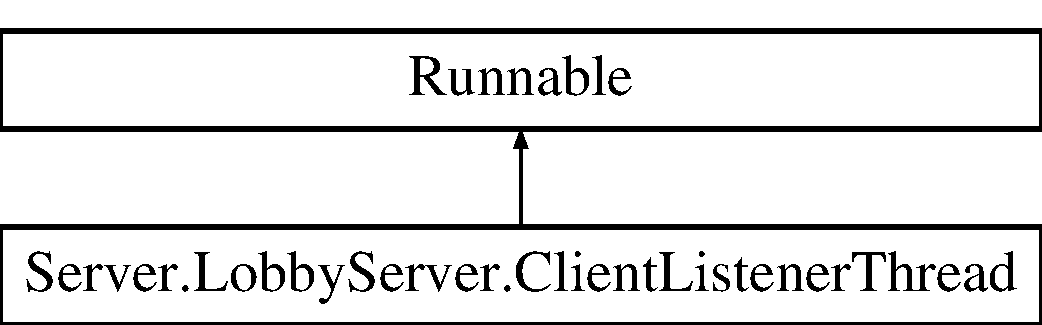
\includegraphics[height=2.000000cm]{a00011}
\end{center}
\end{figure}


\subsubsection{Ausführliche Beschreibung}
Der Thread auf eingehende Clientverbindungen, stellt diese her und instanziiert für jede Verbindung eine Klasse \hyperlink{a00073}{Player}. Dieser wird dann dem \hyperlink{a00054}{Lobby\-Server} übergeben. \begin{DoxyAuthor}{Autor}
Viktoria 
\end{DoxyAuthor}

\hypertarget{a00012}{\subsection{Game\-Lobby Klassenreferenz}
\label{a00012}\index{Game\-Lobby@{Game\-Lobby}}
}


Abgeleitet von J\-Frame und Observer.

\subsubsection*{Öffentliche Methoden}
\begin{DoxyCompactItemize}
\item 
\hypertarget{a00012_af5c160b3c4448522e0d6e0002470c80e}{\hyperlink{a00012_af5c160b3c4448522e0d6e0002470c80e}{Game\-Lobby} ()}\label{a00012_af5c160b3c4448522e0d6e0002470c80e}

\item 
void \hyperlink{a00012_a865971050de64d103900e70b236a0b92}{add\-Start\-Button\-Listener} (Action\-Listener a)
\item 
void \hyperlink{a00012_ab66ade112f82eb29655a140d34bae4fd}{add\-Remove\-Button\-Listener} (Action\-Listener a)
\item 
void \hyperlink{a00012_aac8c97a2425ab3702a82bb0876aa3cc8}{add\-Leave\-Button\-Listener} (Action\-Listener a)
\item 
void \hyperlink{a00012_a1d0d058b74950bbf7305be79b1d60143}{add\-Chat\-Message\-Listener} (Key\-Listener k)
\item 
void \hyperlink{a00012_a9329ba7453dd661d50d2fb8024df3b2b}{set\-Language} (\hyperlink{a00015}{Language} l)
\item 
void \hyperlink{a00012_a2b67d42550fdf9ddd8f3878d0849965c}{update} (Observable o, Object arg)
\item 
void \hyperlink{a00012_a41caffb40957934b02960cf166c78494}{update} (Observable o, String arg)
\end{DoxyCompactItemize}
\subsubsection*{Öffentliche, statische Methoden}
\begin{DoxyCompactItemize}
\item 
\hypertarget{a00012_a8b260eecbaabcef8473fd87ada040682}{static void {\bfseries main} (String\mbox{[}$\,$\mbox{]} args)}\label{a00012_a8b260eecbaabcef8473fd87ada040682}

\end{DoxyCompactItemize}
\subsubsection*{Private Methoden}
\begin{DoxyCompactItemize}
\item 
\hypertarget{a00012_a74cba330cee84fa07487e12fdafe29aa}{void {\bfseries update\-Language} ()}\label{a00012_a74cba330cee84fa07487e12fdafe29aa}

\end{DoxyCompactItemize}
\subsubsection*{Private Attribute}
\begin{DoxyCompactItemize}
\item 
\hypertarget{a00012_aee369a2eca6b8f16ea106cddf68273e8}{J\-Panel {\bfseries content\-Pane}}\label{a00012_aee369a2eca6b8f16ea106cddf68273e8}

\item 
\hypertarget{a00012_aeaa6444a9657e78f8c42051d5f7b4ff6}{J\-Text\-Field {\bfseries message\-Field}}\label{a00012_aeaa6444a9657e78f8c42051d5f7b4ff6}

\item 
\hypertarget{a00012_a430764470b3602491655161cdd67ee8c}{\hyperlink{a00015}{Language} {\bfseries lang}}\label{a00012_a430764470b3602491655161cdd67ee8c}

\item 
\hypertarget{a00012_ad9e9e9e7b8ce2d427def6cc55ef526bd}{J\-Button {\bfseries btn\-Remove\-Player}}\label{a00012_ad9e9e9e7b8ce2d427def6cc55ef526bd}

\item 
\hypertarget{a00012_a1887f14b78aa91b00e5ce42aa504dbe2}{J\-Button {\bfseries btn\-Leave}}\label{a00012_a1887f14b78aa91b00e5ce42aa504dbe2}

\item 
\hypertarget{a00012_a12e216d7d1a56c6e799be1f874c7c82c}{J\-Text\-Area {\bfseries chatlog}}\label{a00012_a12e216d7d1a56c6e799be1f874c7c82c}

\item 
\hypertarget{a00012_a1ac11a30aed65ffc1a336a48515ea9de}{J\-Button {\bfseries btn\-Start\-Game}}\label{a00012_a1ac11a30aed65ffc1a336a48515ea9de}

\end{DoxyCompactItemize}
\subsubsection*{Statische, private Attribute}
\begin{DoxyCompactItemize}
\item 
\hypertarget{a00012_a3238d314ecdee14d2966760945d00c3b}{static final long {\bfseries serial\-Version\-U\-I\-D} = -\/1899311213351027436\-L}\label{a00012_a3238d314ecdee14d2966760945d00c3b}

\end{DoxyCompactItemize}


\subsubsection{Ausführliche Beschreibung}
Die \hyperlink{a00012}{Game\-Lobby} modelliert das Wartefenster, in dem beigetretene Spieler auf den Start des Spieles durch den Spielleiter warten. Der Spielleiter kann Spieler mit dem Remove Player Button entfernen. ueber Leave kehren die Spieler in die \hyperlink{a00016}{Lobby} zurueck. Der spielinterne Chat ist ab hier verfuegbar. 

\subsubsection{Dokumentation der Elementfunktionen}
\hypertarget{a00012_a865971050de64d103900e70b236a0b92}{\index{Client\-::\-View\-::\-Game\-Lobby@{Client\-::\-View\-::\-Game\-Lobby}!add\-Start\-Button\-Listener@{add\-Start\-Button\-Listener}}
\index{add\-Start\-Button\-Listener@{add\-Start\-Button\-Listener}!Client::View::GameLobby@{Client\-::\-View\-::\-Game\-Lobby}}
\paragraph[{add\-Start\-Button\-Listener}]{\setlength{\rightskip}{0pt plus 5cm}void add\-Start\-Button\-Listener (
\begin{DoxyParamCaption}
\item[{Action\-Listener}]{a}
\end{DoxyParamCaption}
)}}\label{a00012_a865971050de64d103900e70b236a0b92}


Fuegt einen Action\-Listener fuer den 'Start \hyperlink{a00011}{Game}' Button hinzu. 


\begin{DoxyParams}{Parameter}
{\em a} & ein Action\-Listener \\
\hline
\end{DoxyParams}
\hypertarget{a00012_ab66ade112f82eb29655a140d34bae4fd}{\index{Client\-::\-View\-::\-Game\-Lobby@{Client\-::\-View\-::\-Game\-Lobby}!add\-Remove\-Button\-Listener@{add\-Remove\-Button\-Listener}}
\index{add\-Remove\-Button\-Listener@{add\-Remove\-Button\-Listener}!Client::View::GameLobby@{Client\-::\-View\-::\-Game\-Lobby}}
\paragraph[{add\-Remove\-Button\-Listener}]{\setlength{\rightskip}{0pt plus 5cm}void add\-Remove\-Button\-Listener (
\begin{DoxyParamCaption}
\item[{Action\-Listener}]{a}
\end{DoxyParamCaption}
)}}\label{a00012_ab66ade112f82eb29655a140d34bae4fd}


Fuegt einen Action\-Listener fuer den 'Remove Player' Button hinzu. 


\begin{DoxyParams}{Parameter}
{\em a} & ein Action\-Listener \\
\hline
\end{DoxyParams}
\hypertarget{a00012_aac8c97a2425ab3702a82bb0876aa3cc8}{\index{Client\-::\-View\-::\-Game\-Lobby@{Client\-::\-View\-::\-Game\-Lobby}!add\-Leave\-Button\-Listener@{add\-Leave\-Button\-Listener}}
\index{add\-Leave\-Button\-Listener@{add\-Leave\-Button\-Listener}!Client::View::GameLobby@{Client\-::\-View\-::\-Game\-Lobby}}
\paragraph[{add\-Leave\-Button\-Listener}]{\setlength{\rightskip}{0pt plus 5cm}void add\-Leave\-Button\-Listener (
\begin{DoxyParamCaption}
\item[{Action\-Listener}]{a}
\end{DoxyParamCaption}
)}}\label{a00012_aac8c97a2425ab3702a82bb0876aa3cc8}


Fuegt einen Action\-Listener fuer den 'Leave' Button hinzu. 


\begin{DoxyParams}{Parameter}
{\em a} & ein Action\-Listener \\
\hline
\end{DoxyParams}
\hypertarget{a00012_a1d0d058b74950bbf7305be79b1d60143}{\index{Client\-::\-View\-::\-Game\-Lobby@{Client\-::\-View\-::\-Game\-Lobby}!add\-Chat\-Message\-Listener@{add\-Chat\-Message\-Listener}}
\index{add\-Chat\-Message\-Listener@{add\-Chat\-Message\-Listener}!Client::View::GameLobby@{Client\-::\-View\-::\-Game\-Lobby}}
\paragraph[{add\-Chat\-Message\-Listener}]{\setlength{\rightskip}{0pt plus 5cm}void add\-Chat\-Message\-Listener (
\begin{DoxyParamCaption}
\item[{Key\-Listener}]{k}
\end{DoxyParamCaption}
)}}\label{a00012_a1d0d058b74950bbf7305be79b1d60143}


Fuet einen Key\-Listener fuer das Nachricht-\/\-Senden-\/\-Feld der \hyperlink{a00016}{Lobby} hinzu. 


\begin{DoxyParams}{Parameter}
{\em k} & \\
\hline
\end{DoxyParams}
\hypertarget{a00012_a9329ba7453dd661d50d2fb8024df3b2b}{\index{Client\-::\-View\-::\-Game\-Lobby@{Client\-::\-View\-::\-Game\-Lobby}!set\-Language@{set\-Language}}
\index{set\-Language@{set\-Language}!Client::View::GameLobby@{Client\-::\-View\-::\-Game\-Lobby}}
\paragraph[{set\-Language}]{\setlength{\rightskip}{0pt plus 5cm}void set\-Language (
\begin{DoxyParamCaption}
\item[{{\bf Language}}]{l}
\end{DoxyParamCaption}
)}}\label{a00012_a9329ba7453dd661d50d2fb8024df3b2b}


Aendert die Sprache des Fensters. 


\begin{DoxyParams}{Parameter}
{\em l} & Sprache in Form des Language-\/\-Enums \\
\hline
\end{DoxyParams}
\hypertarget{a00012_a2b67d42550fdf9ddd8f3878d0849965c}{\index{Client\-::\-View\-::\-Game\-Lobby@{Client\-::\-View\-::\-Game\-Lobby}!update@{update}}
\index{update@{update}!Client::View::GameLobby@{Client\-::\-View\-::\-Game\-Lobby}}
\paragraph[{update}]{\setlength{\rightskip}{0pt plus 5cm}void update (
\begin{DoxyParamCaption}
\item[{Observable}]{o, }
\item[{Object}]{arg}
\end{DoxyParamCaption}
)}}\label{a00012_a2b67d42550fdf9ddd8f3878d0849965c}


Wird durch notify() im \hyperlink{a00003}{Client\-Model} aufgerufen. 

Je nach dem in arg uebergebenen View\-Notification-\/\-Befehl wird ein Update des Fensters ausgefuehrt oder eine Fehlermeldung angezeigt.


\begin{DoxyParams}{Parameter}
{\em o} & erwartet ein Objekt von der Klasse \hyperlink{a00003}{Client\-Model} \\
\hline
{\em arg} & erwartet\-: join\-Game\-Successful, player\-List\-Update, window\-Change\-Forced, game\-Started \\
\hline
\end{DoxyParams}
\hypertarget{a00012_a41caffb40957934b02960cf166c78494}{\index{Client\-::\-View\-::\-Game\-Lobby@{Client\-::\-View\-::\-Game\-Lobby}!update@{update}}
\index{update@{update}!Client::View::GameLobby@{Client\-::\-View\-::\-Game\-Lobby}}
\paragraph[{update}]{\setlength{\rightskip}{0pt plus 5cm}void update (
\begin{DoxyParamCaption}
\item[{Observable}]{o, }
\item[{String}]{arg}
\end{DoxyParamCaption}
)}}\label{a00012_a41caffb40957934b02960cf166c78494}


Wird aufgerufen, wenn eine String-\/\-Nachricht im notify() uebergeben wird. 

Dieser wird als Chatnachricht interpretiert und dem Chatlog angefuegt.


\begin{DoxyParams}{Parameter}
{\em o} & erwartet ein Objekt von der Klasse \hyperlink{a00003}{Client\-Model} \\
\hline
{\em arg} & erwartet einen String, der eine Chatnachricht darstellt \\
\hline
\end{DoxyParams}

\hypertarget{a00013}{\subsection{Ruleset.\-Player\-State Klassenreferenz}
\label{a00013}\index{Ruleset.\-Player\-State@{Ruleset.\-Player\-State}}
}
\subsubsection*{Öffentliche Methoden}
\begin{DoxyCompactItemize}
\item 
String \hyperlink{a00013_a20076c230bb4bfa3404b53bead5194d7}{get\-Name} ()
\item 
Set$<$ \hyperlink{a00001}{Card} $>$ \hyperlink{a00013_ad95ba05e06f70d0ff6f774c3ae1b72b1}{get\-Hand} ()
\item 
\hyperlink{a00012}{Other\-Data} \hyperlink{a00013_ad913d4462ff4019b1d85ba534a27250e}{get\-Other\-Data} ()
\item 
void \hyperlink{a00013_a613eaeb717801aca760df6776d34d228}{add\-Card} (\hyperlink{a00001}{Card} card)
\item 
void \hyperlink{a00013_a38c66bb85292eaedd970cb1c6bc38dca}{remove\-Card} (\hyperlink{a00001}{Card} card)
\end{DoxyCompactItemize}


\subsubsection{Dokumentation der Elementfunktionen}
\hypertarget{a00013_a613eaeb717801aca760df6776d34d228}{\index{Ruleset\-::\-Player\-State@{Ruleset\-::\-Player\-State}!add\-Card@{add\-Card}}
\index{add\-Card@{add\-Card}!Ruleset::PlayerState@{Ruleset\-::\-Player\-State}}
\paragraph[{add\-Card}]{\setlength{\rightskip}{0pt plus 5cm}void Ruleset.\-Player\-State.\-add\-Card (
\begin{DoxyParamCaption}
\item[{{\bf Card}}]{card}
\end{DoxyParamCaption}
)}}\label{a00013_a613eaeb717801aca760df6776d34d228}


Gibt dem Spieler eine Karte. 


\begin{DoxyParams}{Parameter}
{\em card} & Die Karte die dem Spieler gegeben wird \\
\hline
\end{DoxyParams}
\hypertarget{a00013_ad95ba05e06f70d0ff6f774c3ae1b72b1}{\index{Ruleset\-::\-Player\-State@{Ruleset\-::\-Player\-State}!get\-Hand@{get\-Hand}}
\index{get\-Hand@{get\-Hand}!Ruleset::PlayerState@{Ruleset\-::\-Player\-State}}
\paragraph[{get\-Hand}]{\setlength{\rightskip}{0pt plus 5cm}Set$<${\bf Card}$>$ Ruleset.\-Player\-State.\-get\-Hand (
\begin{DoxyParamCaption}
{}
\end{DoxyParamCaption}
)}}\label{a00013_ad95ba05e06f70d0ff6f774c3ae1b72b1}


Holt die Kartenhand des Spielers. 

\begin{DoxyReturn}{Rückgabe}
own\-Hand Die Kartenhand des Spielers 
\end{DoxyReturn}
\hypertarget{a00013_a20076c230bb4bfa3404b53bead5194d7}{\index{Ruleset\-::\-Player\-State@{Ruleset\-::\-Player\-State}!get\-Name@{get\-Name}}
\index{get\-Name@{get\-Name}!Ruleset::PlayerState@{Ruleset\-::\-Player\-State}}
\paragraph[{get\-Name}]{\setlength{\rightskip}{0pt plus 5cm}String Ruleset.\-Player\-State.\-get\-Name (
\begin{DoxyParamCaption}
{}
\end{DoxyParamCaption}
)}}\label{a00013_a20076c230bb4bfa3404b53bead5194d7}


Holt den namen eines Spielers. 

\begin{DoxyReturn}{Rückgabe}
name Der Name des Spielers 
\end{DoxyReturn}
\hypertarget{a00013_ad913d4462ff4019b1d85ba534a27250e}{\index{Ruleset\-::\-Player\-State@{Ruleset\-::\-Player\-State}!get\-Other\-Data@{get\-Other\-Data}}
\index{get\-Other\-Data@{get\-Other\-Data}!Ruleset::PlayerState@{Ruleset\-::\-Player\-State}}
\paragraph[{get\-Other\-Data}]{\setlength{\rightskip}{0pt plus 5cm}{\bf Other\-Data} Ruleset.\-Player\-State.\-get\-Other\-Data (
\begin{DoxyParamCaption}
{}
\end{DoxyParamCaption}
)}}\label{a00013_ad913d4462ff4019b1d85ba534a27250e}


Holt die zus�tzlichen Informationen des Spielers. 

\begin{DoxyReturn}{Rückgabe}
own\-Hand Die zus�tzlichen Informationen des Spielers 
\end{DoxyReturn}
\hypertarget{a00013_a38c66bb85292eaedd970cb1c6bc38dca}{\index{Ruleset\-::\-Player\-State@{Ruleset\-::\-Player\-State}!remove\-Card@{remove\-Card}}
\index{remove\-Card@{remove\-Card}!Ruleset::PlayerState@{Ruleset\-::\-Player\-State}}
\paragraph[{remove\-Card}]{\setlength{\rightskip}{0pt plus 5cm}void Ruleset.\-Player\-State.\-remove\-Card (
\begin{DoxyParamCaption}
\item[{{\bf Card}}]{card}
\end{DoxyParamCaption}
)}}\label{a00013_a38c66bb85292eaedd970cb1c6bc38dca}


Entfernt eine Karte aus der Hand des Spielers. 


\begin{DoxyParams}{Parameter}
{\em card} & \\
\hline
\end{DoxyParams}

\hypertarget{a00014}{\subsection{Input\-Number Klassenreferenz}
\label{a00014}\index{Input\-Number@{Input\-Number}}
}


Abgeleitet von Observer.

\subsubsection*{Öffentliche Methoden}
\begin{DoxyCompactItemize}
\item 
void \hyperlink{a00014_a2b67d42550fdf9ddd8f3878d0849965c}{update} (Observable o, Object arg)
\end{DoxyCompactItemize}
\subsubsection*{Private Attribute}
\begin{DoxyCompactItemize}
\item 
\hypertarget{a00014_a6d8bcbe4ebb8e887e3dccb18c9ce3ad7}{Object {\bfseries number\-Textfield}}\label{a00014_a6d8bcbe4ebb8e887e3dccb18c9ce3ad7}

\end{DoxyCompactItemize}


\subsubsection{Ausführliche Beschreibung}
In diesem Fenster, kann der Benutzer eine Zahl eingeben. 

\subsubsection{Dokumentation der Elementfunktionen}
\hypertarget{a00014_a2b67d42550fdf9ddd8f3878d0849965c}{\index{Client\-::\-View\-::\-Input\-Number@{Client\-::\-View\-::\-Input\-Number}!update@{update}}
\index{update@{update}!Client::View::InputNumber@{Client\-::\-View\-::\-Input\-Number}}
\paragraph[{update}]{\setlength{\rightskip}{0pt plus 5cm}void update (
\begin{DoxyParamCaption}
\item[{Observable}]{o, }
\item[{Object}]{arg}
\end{DoxyParamCaption}
)}}\label{a00014_a2b67d42550fdf9ddd8f3878d0849965c}


Wird durch notify() im \hyperlink{a00003}{Client\-Model} aufgerufen. 

Je nach dem in arg uebergebenen Befehl wird ein Update des Fensters ausgefuehrt oder eine Fehlermeldung angezeigt.


\begin{DoxyParams}{Parameter}
{\em o} & erwartet ein Objekt von der Klasse \hyperlink{a00003}{Client\-Model} \\
\hline
{\em arg} & erwartet\-: open\-Input\-Number, input\-Number\-Successful \\
\hline
\end{DoxyParams}

\hypertarget{a00015}{\subsection{Client.\-Client\-State Enum-\/\-Referenz}
\label{a00015}\index{Client.\-Client\-State@{Client.\-Client\-State}}
}

\hypertarget{a00016}{\subsection{Ruleset.\-Server\-Ruleset Klassenreferenz}
\label{a00016}\index{Ruleset.\-Server\-Ruleset@{Ruleset.\-Server\-Ruleset}}
}
Klassendiagramm für Ruleset.\-Server\-Ruleset\-:\begin{figure}[H]
\begin{center}
\leavevmode
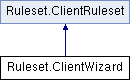
\includegraphics[height=2.000000cm]{a00016}
\end{center}
\end{figure}
\subsubsection*{Öffentliche Methoden}
\begin{DoxyCompactItemize}
\item 
\hyperlink{a00013}{Player\-State} \hyperlink{a00016_a473a55c851bbda707b25948c39334a8a}{get\-Current\-Player} ()
\item 
\hyperlink{a00013}{Player\-State} \hyperlink{a00016_a4a5e3a0fa28ba2bd563224d875f5835c}{get\-Player\-State} (String name)
\item 
void \hyperlink{a00016_afcfbddd7397a6043913b5e742934d2c2}{resolve\-Message} (Msg\-Card msg\-Card, String name)
\item 
void \hyperlink{a00016_ac639a8d99c0e2243f9f3fe565a315c51}{resolve\-Message} (Msg\-Multi\-Cards msg\-Multi\-Card, String name)
\item 
void \hyperlink{a00016_a9f1a95cc9488d8a9519ce69718f91322}{resolve\-Message} (Msg\-Number msg\-Number, String name)
\item 
void \hyperlink{a00016_ada2667ea093481a58f253f43ff6cc49f}{resolve\-Message} (Msg\-Selection msg\-Selection, String name)
\end{DoxyCompactItemize}


\subsubsection{Ausführliche Beschreibung}
Das \hyperlink{a00016}{Server\-Ruleset} wird im Game\-Server instanziert und verwaltet die Zust�nde des Game\-States im Server. Mit der Methode \hyperlink{a00016_aa49663b89f89b9f7b3685f0b96560f69}{is\-Valid\-Move()} wird eine Eingabe eines Clients auf Regelkonformit�t �berpr�ft und dann im Game\-Server das \hyperlink{a00008}{Game\-State} ver�ndert. �ber \hyperlink{a00016_afcfbddd7397a6043913b5e742934d2c2}{resolve\-Message()} kann eine Game\-Serverinstanz eine Ruleset\-Message vom Player an das Ruleset weiterleiten. 

\subsubsection{Dokumentation der Elementfunktionen}
\hypertarget{a00016_a473a55c851bbda707b25948c39334a8a}{\index{Ruleset\-::\-Server\-Ruleset@{Ruleset\-::\-Server\-Ruleset}!get\-Current\-Player@{get\-Current\-Player}}
\index{get\-Current\-Player@{get\-Current\-Player}!Ruleset::ServerRuleset@{Ruleset\-::\-Server\-Ruleset}}
\paragraph[{get\-Current\-Player}]{\setlength{\rightskip}{0pt plus 5cm}{\bf Player\-State} Ruleset.\-Server\-Ruleset.\-get\-Current\-Player (
\begin{DoxyParamCaption}
{}
\end{DoxyParamCaption}
)}}\label{a00016_a473a55c851bbda707b25948c39334a8a}


Holt den Spieler der gerade am Zug ist. 

\begin{DoxyReturn}{Rückgabe}
current\-Player Der Spielzustand des Spielers der grad am Zug ist 
\end{DoxyReturn}
\hypertarget{a00016_a4a5e3a0fa28ba2bd563224d875f5835c}{\index{Ruleset\-::\-Server\-Ruleset@{Ruleset\-::\-Server\-Ruleset}!get\-Player\-State@{get\-Player\-State}}
\index{get\-Player\-State@{get\-Player\-State}!Ruleset::ServerRuleset@{Ruleset\-::\-Server\-Ruleset}}
\paragraph[{get\-Player\-State}]{\setlength{\rightskip}{0pt plus 5cm}{\bf Player\-State} Ruleset.\-Server\-Ruleset.\-get\-Player\-State (
\begin{DoxyParamCaption}
\item[{String}]{name}
\end{DoxyParamCaption}
)}}\label{a00016_a4a5e3a0fa28ba2bd563224d875f5835c}


Holt den Spielerzustand eines Spielers. 


\begin{DoxyParams}{Parameter}
{\em name} & Der Name des Spielers \\
\hline
\end{DoxyParams}
\begin{DoxyReturn}{Rückgabe}
player\-State Spielzustand eines Spielers 
\end{DoxyReturn}
\hypertarget{a00016_afcfbddd7397a6043913b5e742934d2c2}{\index{Ruleset\-::\-Server\-Ruleset@{Ruleset\-::\-Server\-Ruleset}!resolve\-Message@{resolve\-Message}}
\index{resolve\-Message@{resolve\-Message}!Ruleset::ServerRuleset@{Ruleset\-::\-Server\-Ruleset}}
\paragraph[{resolve\-Message}]{\setlength{\rightskip}{0pt plus 5cm}void Ruleset.\-Server\-Ruleset.\-resolve\-Message (
\begin{DoxyParamCaption}
\item[{Msg\-Card}]{msg\-Card, }
\item[{String}]{name}
\end{DoxyParamCaption}
)}}\label{a00016_afcfbddd7397a6043913b5e742934d2c2}


Verarbeitet die Ruleset\-Message dass eine Karte vom Spieler gespielt. 


\begin{DoxyParams}{Parameter}
{\em msg\-Card} & Die Nachricht vom Client welche Karte gespielt wurde \\
\hline
{\em name} & Der Name des Spielers \\
\hline
\end{DoxyParams}
\hypertarget{a00016_ac639a8d99c0e2243f9f3fe565a315c51}{\index{Ruleset\-::\-Server\-Ruleset@{Ruleset\-::\-Server\-Ruleset}!resolve\-Message@{resolve\-Message}}
\index{resolve\-Message@{resolve\-Message}!Ruleset::ServerRuleset@{Ruleset\-::\-Server\-Ruleset}}
\paragraph[{resolve\-Message}]{\setlength{\rightskip}{0pt plus 5cm}void Ruleset.\-Server\-Ruleset.\-resolve\-Message (
\begin{DoxyParamCaption}
\item[{Msg\-Multi\-Cards}]{msg\-Multi\-Card, }
\item[{String}]{name}
\end{DoxyParamCaption}
)}}\label{a00016_ac639a8d99c0e2243f9f3fe565a315c51}


Verarbeitet die Ruleset\-Message dass mehrere Karten von einem Spieler �bergeben wurden. 


\begin{DoxyParams}{Parameter}
{\em msg\-Multi\-Card} & Die Nachricht vom Client \\
\hline
{\em name} & Der Name des Spielers \\
\hline
\end{DoxyParams}
\hypertarget{a00016_a9f1a95cc9488d8a9519ce69718f91322}{\index{Ruleset\-::\-Server\-Ruleset@{Ruleset\-::\-Server\-Ruleset}!resolve\-Message@{resolve\-Message}}
\index{resolve\-Message@{resolve\-Message}!Ruleset::ServerRuleset@{Ruleset\-::\-Server\-Ruleset}}
\paragraph[{resolve\-Message}]{\setlength{\rightskip}{0pt plus 5cm}void Ruleset.\-Server\-Ruleset.\-resolve\-Message (
\begin{DoxyParamCaption}
\item[{Msg\-Number}]{msg\-Number, }
\item[{String}]{name}
\end{DoxyParamCaption}
)}}\label{a00016_a9f1a95cc9488d8a9519ce69718f91322}


Verarbeitet die Ruleset\-Message dass ein Spieler eine Stichangabe gemacht hat. 


\begin{DoxyParams}{Parameter}
{\em msg\-Number} & Die Nachricht vom Client \\
\hline
{\em name} & Der Name des Spielers \\
\hline
\end{DoxyParams}
\hypertarget{a00016_ada2667ea093481a58f253f43ff6cc49f}{\index{Ruleset\-::\-Server\-Ruleset@{Ruleset\-::\-Server\-Ruleset}!resolve\-Message@{resolve\-Message}}
\index{resolve\-Message@{resolve\-Message}!Ruleset::ServerRuleset@{Ruleset\-::\-Server\-Ruleset}}
\paragraph[{resolve\-Message}]{\setlength{\rightskip}{0pt plus 5cm}void Ruleset.\-Server\-Ruleset.\-resolve\-Message (
\begin{DoxyParamCaption}
\item[{Msg\-Selection}]{msg\-Selection, }
\item[{String}]{name}
\end{DoxyParamCaption}
)}}\label{a00016_ada2667ea093481a58f253f43ff6cc49f}


Verarbeitet die Ruleset\-Message dass ein Spieler eine Farbe ausgew�hlt hat. 


\begin{DoxyParams}{Parameter}
{\em msg\-Selection} & Die Nachricht vom Client \\
\hline
{\em name} & \\
\hline
\end{DoxyParams}

\hypertarget{a00017}{\subsection{Ruleset.\-Server\-Wizard Klassenreferenz}
\label{a00017}\index{Ruleset.\-Server\-Wizard@{Ruleset.\-Server\-Wizard}}
}
Klassendiagramm für Ruleset.\-Server\-Wizard\-:\begin{figure}[H]
\begin{center}
\leavevmode
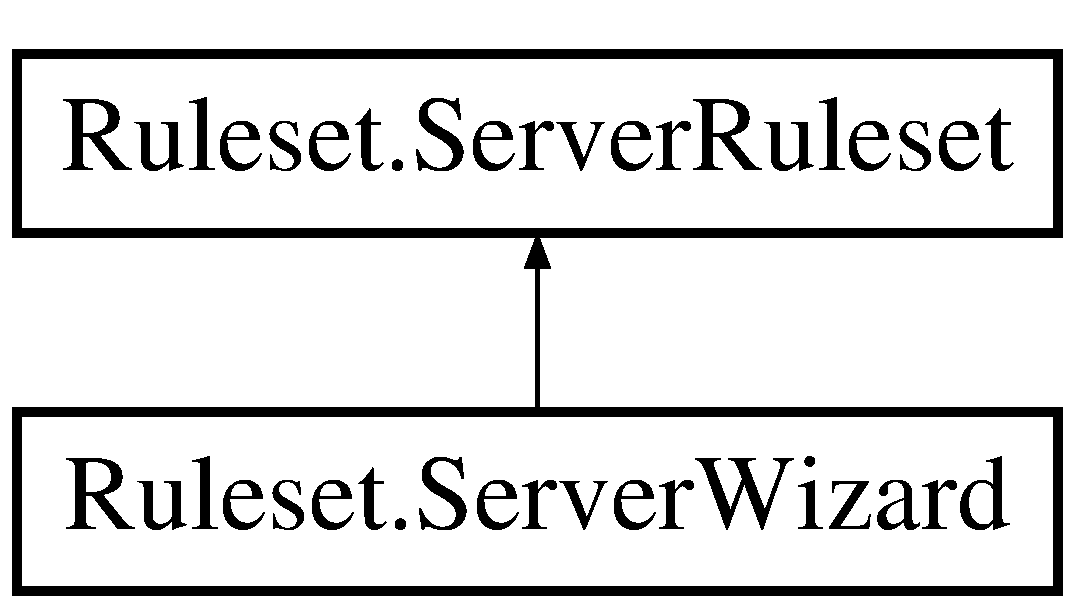
\includegraphics[height=2.000000cm]{a00017}
\end{center}
\end{figure}
\subsubsection*{Öffentliche Methoden}
\begin{DoxyCompactItemize}
\item 
boolean \hyperlink{a00017_af079641e9a83d29de9e1ac868a0af202}{is\-Valid\-Move} (\hyperlink{a00001}{Card} card)
\end{DoxyCompactItemize}


\subsubsection{Dokumentation der Elementfunktionen}
\hypertarget{a00017_af079641e9a83d29de9e1ac868a0af202}{\index{Ruleset\-::\-Server\-Wizard@{Ruleset\-::\-Server\-Wizard}!is\-Valid\-Move@{is\-Valid\-Move}}
\index{is\-Valid\-Move@{is\-Valid\-Move}!Ruleset::ServerWizard@{Ruleset\-::\-Server\-Wizard}}
\paragraph[{is\-Valid\-Move}]{\setlength{\rightskip}{0pt plus 5cm}boolean Ruleset.\-Server\-Wizard.\-is\-Valid\-Move (
\begin{DoxyParamCaption}
\item[{{\bf Card}}]{card}
\end{DoxyParamCaption}
)\hspace{0.3cm}{\ttfamily [virtual]}}}\label{a00017_af079641e9a83d29de9e1ac868a0af202}


Pr�ft ob ein gemachter Zug in einem Wizard Spiel g�ltig ist. 

\begin{DoxyReturn}{Rückgabe}
is\-Valid true falls Zug g�ltig, false wenn nicht 
\end{DoxyReturn}


Implementiert \hyperlink{a00016_aa49663b89f89b9f7b3685f0b96560f69}{Ruleset.\-Server\-Ruleset}.


\hypertarget{a00018}{\subsection{Other\-Player Klassenreferenz}
\label{a00018}\index{Other\-Player@{Other\-Player}}
}
\subsubsection*{Private Attribute}
\begin{DoxyCompactItemize}
\item 
\hypertarget{a00018_a46ff4804e1f3b2aa954327b7ebaedb5f}{Object {\bfseries name}}\label{a00018_a46ff4804e1f3b2aa954327b7ebaedb5f}

\item 
\hypertarget{a00018_a479739d676f2040870ad5be69a6c8a9e}{Object {\bfseries info}}\label{a00018_a479739d676f2040870ad5be69a6c8a9e}

\end{DoxyCompactItemize}


\subsubsection{Ausführliche Beschreibung}
Zeigt die Informationen über die anderen Spieler an, also den Namen, ein Symbol für die verdeckte Hand und das Label für zusaetzliche Angaben. 
\hypertarget{a00019}{\subsection{Own\-Hand Klassenreferenz}
\label{a00019}\index{Own\-Hand@{Own\-Hand}}
}
\subsubsection*{Private Attribute}
\begin{DoxyCompactItemize}
\item 
\hypertarget{a00019_a9233afadd1e46e11f03ea518e9c86366}{Object {\bfseries cards}}\label{a00019_a9233afadd1e46e11f03ea518e9c86366}

\item 
\hypertarget{a00019_a32963d9bbf9a4ad1ca8d0e1cf6c54bfe}{Set$<$ \hyperlink{a00022}{View\-Card} $>$ {\bfseries card}}\label{a00019_a32963d9bbf9a4ad1ca8d0e1cf6c54bfe}

\end{DoxyCompactItemize}


\subsubsection{Ausführliche Beschreibung}
Stellt die Karten dar, die der Spieler auf der Hand hat. Der Spieler kann eine Karte durch Anklicken auswaehlen und durch einen zweiten Klick ausspielen. 
\hypertarget{a00020}{\subsection{Com\-Objects.\-Com\-Client\-Leave Klassenreferenz}
\label{a00020}\index{Com\-Objects.\-Com\-Client\-Leave@{Com\-Objects.\-Com\-Client\-Leave}}
}
Klassendiagramm für Com\-Objects.\-Com\-Client\-Leave\-:\begin{figure}[H]
\begin{center}
\leavevmode
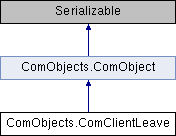
\includegraphics[height=3.000000cm]{a00020}
\end{center}
\end{figure}


\subsubsection{Ausführliche Beschreibung}
Sie wird zur Benachrichtigung gesendet, wenn ein Spieler ins nächste Fenster möchte und aus dem alten entfernt werden soll. 
\hypertarget{a00021}{\subsection{Score\-Window Klassenreferenz}
\label{a00021}\index{Score\-Window@{Score\-Window}}
}


Abgeleitet von Observer.

\subsubsection*{Öffentliche Methoden}
\begin{DoxyCompactItemize}
\item 
void \hyperlink{a00021_a2b67d42550fdf9ddd8f3878d0849965c}{update} (Observable o, Object arg)
\end{DoxyCompactItemize}


\subsubsection{Ausführliche Beschreibung}
Dieses Fenster zeigt den momentanen Punktestand nach jeder Runde und den Gesamtpunktestand am Ende des Spieles an. 

\subsubsection{Dokumentation der Elementfunktionen}
\hypertarget{a00021_a2b67d42550fdf9ddd8f3878d0849965c}{\index{Client\-::\-View\-::\-Score\-Window@{Client\-::\-View\-::\-Score\-Window}!update@{update}}
\index{update@{update}!Client::View::ScoreWindow@{Client\-::\-View\-::\-Score\-Window}}
\paragraph[{update}]{\setlength{\rightskip}{0pt plus 5cm}void update (
\begin{DoxyParamCaption}
\item[{Observable}]{o, }
\item[{Object}]{arg}
\end{DoxyParamCaption}
)}}\label{a00021_a2b67d42550fdf9ddd8f3878d0849965c}


Wird durch notify() im \hyperlink{a00003}{Client\-Model} aufgerufen. 

Je nach dem in arg uebergebenen Befehl wird ein Update des Fensters ausgefuehrt oder eine Fehlermeldung angezeigt.


\begin{DoxyParams}{Parameter}
{\em o} & erwartet ein Objekt von der Klasse \hyperlink{a00003}{Client\-Model} \\
\hline
{\em arg} & erwartet\-: show\-Score \\
\hline
\end{DoxyParams}

\hypertarget{a00022}{\subsection{View\-Card Klassenreferenz}
\label{a00022}\index{View\-Card@{View\-Card}}
}


Abgeleitet von J\-Panel.

\subsubsection*{Öffentliche Methoden}
\begin{DoxyCompactItemize}
\item 
\hyperlink{a00022_a682302cb58c058e170ea714a45c2342c}{View\-Card} (String s, int n)
\item 
int \hyperlink{a00022_aea93026f92028ac88f6b60cd2f3e438b}{get\-I\-D} ()
\item 
\hypertarget{a00022_aac9233d06f3c093fc37139d7d2b258f6}{void {\bfseries paint\-Component} (Graphics g)}\label{a00022_aac9233d06f3c093fc37139d7d2b258f6}

\end{DoxyCompactItemize}
\subsubsection*{Private Attribute}
\begin{DoxyCompactItemize}
\item 
\hypertarget{a00022_adb85e16ac8c9f62df2d33b1262649843}{String {\bfseries path}}\label{a00022_adb85e16ac8c9f62df2d33b1262649843}

\item 
\hypertarget{a00022_a7441ef0865bcb3db9b8064dd7375c1ea}{int {\bfseries id}}\label{a00022_a7441ef0865bcb3db9b8064dd7375c1ea}

\item 
\hypertarget{a00022_a9d8fedf4068416562cae5761080e4792}{Buffered\-Image {\bfseries face}}\label{a00022_a9d8fedf4068416562cae5761080e4792}

\end{DoxyCompactItemize}
\subsubsection*{Statische, private Attribute}
\begin{DoxyCompactItemize}
\item 
\hypertarget{a00022_a3238d314ecdee14d2966760945d00c3b}{static final long {\bfseries serial\-Version\-U\-I\-D} = 8733682958484899430\-L}\label{a00022_a3238d314ecdee14d2966760945d00c3b}

\end{DoxyCompactItemize}


\subsubsection{Ausführliche Beschreibung}
\hyperlink{a00022}{View\-Card} ist die View-\/seitige Repraesentation einer Karte. Sie wird verwendet um einzelne Karten auf das Spielfeld zu zeichnen. Dazu enthaelt sie die Pfadangabe zu dem Ordner, in dem die Bilder der Karten gespeichert sind, und eine I\-D, um das genaue Bild zu spezifizieren. 

\subsubsection{Beschreibung der Konstruktoren und Destruktoren}
\hypertarget{a00022_a682302cb58c058e170ea714a45c2342c}{\index{Client\-::\-View\-::\-View\-Card@{Client\-::\-View\-::\-View\-Card}!View\-Card@{View\-Card}}
\index{View\-Card@{View\-Card}!Client::View::ViewCard@{Client\-::\-View\-::\-View\-Card}}
\paragraph[{View\-Card}]{\setlength{\rightskip}{0pt plus 5cm}{\bf View\-Card} (
\begin{DoxyParamCaption}
\item[{String}]{s, }
\item[{int}]{n}
\end{DoxyParamCaption}
)}}\label{a00022_a682302cb58c058e170ea714a45c2342c}


Erstellt eine neue Karte fuer die Anzeige und zeichnet dafuer das Bild, das durch die Pfadangabe s und seine Kardinaliaet n im Ordner angegeben ist. 

Die Pfadangabe wird durch das Regelwerk bestimmt.


\begin{DoxyParams}{Parameter}
{\em s} & Pfadangabe zum zu zeichnenden Bild \\
\hline
{\em n} & I\-D der Karte \\
\hline
\end{DoxyParams}


\subsubsection{Dokumentation der Elementfunktionen}
\hypertarget{a00022_aea93026f92028ac88f6b60cd2f3e438b}{\index{Client\-::\-View\-::\-View\-Card@{Client\-::\-View\-::\-View\-Card}!get\-I\-D@{get\-I\-D}}
\index{get\-I\-D@{get\-I\-D}!Client::View::ViewCard@{Client\-::\-View\-::\-View\-Card}}
\paragraph[{get\-I\-D}]{\setlength{\rightskip}{0pt plus 5cm}int get\-I\-D (
\begin{DoxyParamCaption}
{}
\end{DoxyParamCaption}
)}}\label{a00022_aea93026f92028ac88f6b60cd2f3e438b}


Gibt die I\-D der Karte zurueck. 

\begin{DoxyReturn}{Rückgabe}
I\-D der Karte 
\end{DoxyReturn}

\hypertarget{a00023}{\subsection{Warning Klassenreferenz}
\label{a00023}\index{Warning@{Warning}}
}


Abgeleitet von Observer.

\subsubsection*{Öffentliche Methoden}
\begin{DoxyCompactItemize}
\item 
void \hyperlink{a00023_a1f0025961cc745f47ae48ba98ffad7bf}{set\-Text} (String text)
\item 
void \hyperlink{a00023_a2b67d42550fdf9ddd8f3878d0849965c}{update} (Observable o, Object arg)
\end{DoxyCompactItemize}
\subsubsection*{Private Attribute}
\begin{DoxyCompactItemize}
\item 
\hypertarget{a00023_a7e805d5872b3c74587fd7af4be6091fd}{String {\bfseries warning\-Text}}\label{a00023_a7e805d5872b3c74587fd7af4be6091fd}

\end{DoxyCompactItemize}


\subsubsection{Ausführliche Beschreibung}
Das Warning-\/\-Fenster zeigt dem Benutzer Fehlermeldungen bzw. Hinweise an, welche vom \hyperlink{a00003}{Client\-Model} uebergeben wurden. Es wird nur im Fehlerfall angezeigt. 

\subsubsection{Dokumentation der Elementfunktionen}
\hypertarget{a00023_a1f0025961cc745f47ae48ba98ffad7bf}{\index{Client\-::\-View\-::\-Warning@{Client\-::\-View\-::\-Warning}!set\-Text@{set\-Text}}
\index{set\-Text@{set\-Text}!Client::View::Warning@{Client\-::\-View\-::\-Warning}}
\paragraph[{set\-Text}]{\setlength{\rightskip}{0pt plus 5cm}void set\-Text (
\begin{DoxyParamCaption}
\item[{String}]{text}
\end{DoxyParamCaption}
)}}\label{a00023_a1f0025961cc745f47ae48ba98ffad7bf}


Setzt den Warnhinweis des Fensters. 


\begin{DoxyParams}{Parameter}
{\em text} & Warnhinweis, der angezeigt werden soll \\
\hline
\end{DoxyParams}
\hypertarget{a00023_a2b67d42550fdf9ddd8f3878d0849965c}{\index{Client\-::\-View\-::\-Warning@{Client\-::\-View\-::\-Warning}!update@{update}}
\index{update@{update}!Client::View::Warning@{Client\-::\-View\-::\-Warning}}
\paragraph[{update}]{\setlength{\rightskip}{0pt plus 5cm}void update (
\begin{DoxyParamCaption}
\item[{Observable}]{o, }
\item[{Object}]{arg}
\end{DoxyParamCaption}
)}}\label{a00023_a2b67d42550fdf9ddd8f3878d0849965c}


Wird durch notify() im \hyperlink{a00003}{Client\-Model} aufgerufen. 

Je nach dem in arg übergebenen Befehl wird ein Update des Fensters ausgeführt oder eine Fehlermeldung angezeigt.


\begin{DoxyParams}{Parameter}
{\em o} & erwartet ein Objekt von der Klasse \hyperlink{a00003}{Client\-Model} \\
\hline
{\em arg} & erwartet\-: open\-Warning \\
\hline
\end{DoxyParams}

\hypertarget{a00024}{\subsection{Com\-Objects.\-Com\-Init\-Lobby Klassenreferenz}
\label{a00024}\index{Com\-Objects.\-Com\-Init\-Lobby@{Com\-Objects.\-Com\-Init\-Lobby}}
}
Klassendiagramm für Com\-Objects.\-Com\-Init\-Lobby\-:\begin{figure}[H]
\begin{center}
\leavevmode
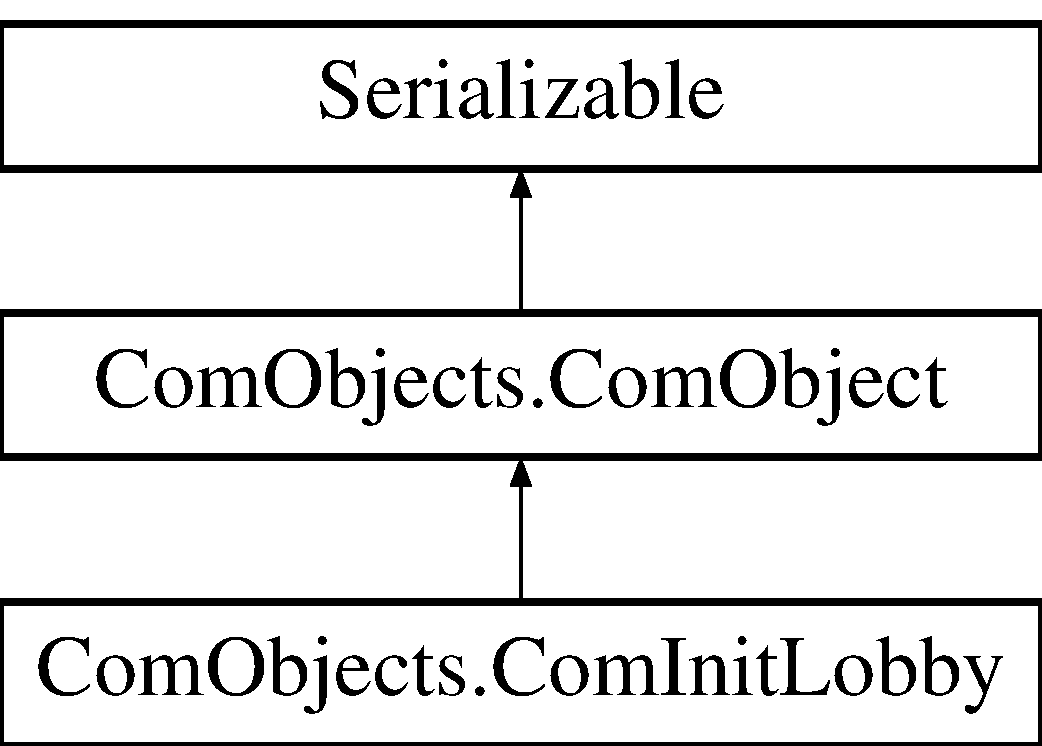
\includegraphics[height=3.000000cm]{a00024}
\end{center}
\end{figure}
\subsubsection*{Öffentliche Methoden}
\begin{DoxyCompactItemize}
\item 
\hyperlink{a00024_a6dd7844ead6be6ad10308dada6dfb77c}{Com\-Init\-Lobby} (List player\-List, Set game\-List)
\item 
List \hyperlink{a00024_afbb8f13abe20cdd44a14bf2174f89b65}{get\-Player\-List} ()
\item 
Set$<$ \hyperlink{a00044}{Game\-Server\-Representation} $>$ \hyperlink{a00024_a2fa7410dcaccbf82e10daab9650fe3b3}{get\-Game\-List} ()
\end{DoxyCompactItemize}


\subsubsection{Ausführliche Beschreibung}
Sie synchronisiert den Client mit der Lobby, wenn er sich mit dem Server verbindet oder nach einem Spiel in die Lobby zurückkehrt. Dazu enthält sie sowohl die player\-List, als auch die game\-List. 

\subsubsection{Beschreibung der Konstruktoren und Destruktoren}
\hypertarget{a00024_a6dd7844ead6be6ad10308dada6dfb77c}{\index{Com\-Objects\-::\-Com\-Init\-Lobby@{Com\-Objects\-::\-Com\-Init\-Lobby}!Com\-Init\-Lobby@{Com\-Init\-Lobby}}
\index{Com\-Init\-Lobby@{Com\-Init\-Lobby}!ComObjects::ComInitLobby@{Com\-Objects\-::\-Com\-Init\-Lobby}}
\paragraph[{Com\-Init\-Lobby}]{\setlength{\rightskip}{0pt plus 5cm}Com\-Objects.\-Com\-Init\-Lobby.\-Com\-Init\-Lobby (
\begin{DoxyParamCaption}
\item[{List}]{player\-List, }
\item[{Set}]{game\-List}
\end{DoxyParamCaption}
)}}\label{a00024_a6dd7844ead6be6ad10308dada6dfb77c}


Dies ist der Kontruktor für eine neue Com\-Init\-Lobby-\/\-Nachricht. 


\begin{DoxyParams}{Parameter}
{\em player\-List} & ist die Liste der Spieler, die sich in der Lobby befinden. \\
\hline
{\em game\-List} & ist die Liste der Spiele, die existieren und in der Lobby angezeigt werden. \\
\hline
\end{DoxyParams}


\subsubsection{Dokumentation der Elementfunktionen}
\hypertarget{a00024_a2fa7410dcaccbf82e10daab9650fe3b3}{\index{Com\-Objects\-::\-Com\-Init\-Lobby@{Com\-Objects\-::\-Com\-Init\-Lobby}!get\-Game\-List@{get\-Game\-List}}
\index{get\-Game\-List@{get\-Game\-List}!ComObjects::ComInitLobby@{Com\-Objects\-::\-Com\-Init\-Lobby}}
\paragraph[{get\-Game\-List}]{\setlength{\rightskip}{0pt plus 5cm}Set$<${\bf Game\-Server\-Representation}$>$ Com\-Objects.\-Com\-Init\-Lobby.\-get\-Game\-List (
\begin{DoxyParamCaption}
{}
\end{DoxyParamCaption}
)}}\label{a00024_a2fa7410dcaccbf82e10daab9650fe3b3}


Diese Methode liefert eine Liste aller Spiele, die erstellt wurden, damit sie in der Lobby angezeigt werden können. 

\begin{DoxyReturn}{Rückgabe}
die Liste der Spiele. 
\end{DoxyReturn}
\hypertarget{a00024_afbb8f13abe20cdd44a14bf2174f89b65}{\index{Com\-Objects\-::\-Com\-Init\-Lobby@{Com\-Objects\-::\-Com\-Init\-Lobby}!get\-Player\-List@{get\-Player\-List}}
\index{get\-Player\-List@{get\-Player\-List}!ComObjects::ComInitLobby@{Com\-Objects\-::\-Com\-Init\-Lobby}}
\paragraph[{get\-Player\-List}]{\setlength{\rightskip}{0pt plus 5cm}List Com\-Objects.\-Com\-Init\-Lobby.\-get\-Player\-List (
\begin{DoxyParamCaption}
{}
\end{DoxyParamCaption}
)}}\label{a00024_afbb8f13abe20cdd44a14bf2174f89b65}


Die Methode liefert die Liste aller Spieler, die in der Lobby sind. 

\begin{DoxyReturn}{Rückgabe}
die Liste der Spieler. 
\end{DoxyReturn}

\hypertarget{a00025}{\subsection{Com\-Objects.\-Com\-Join\-Request Klassenreferenz}
\label{a00025}\index{Com\-Objects.\-Com\-Join\-Request@{Com\-Objects.\-Com\-Join\-Request}}
}
Klassendiagramm für Com\-Objects.\-Com\-Join\-Request\-:\begin{figure}[H]
\begin{center}
\leavevmode
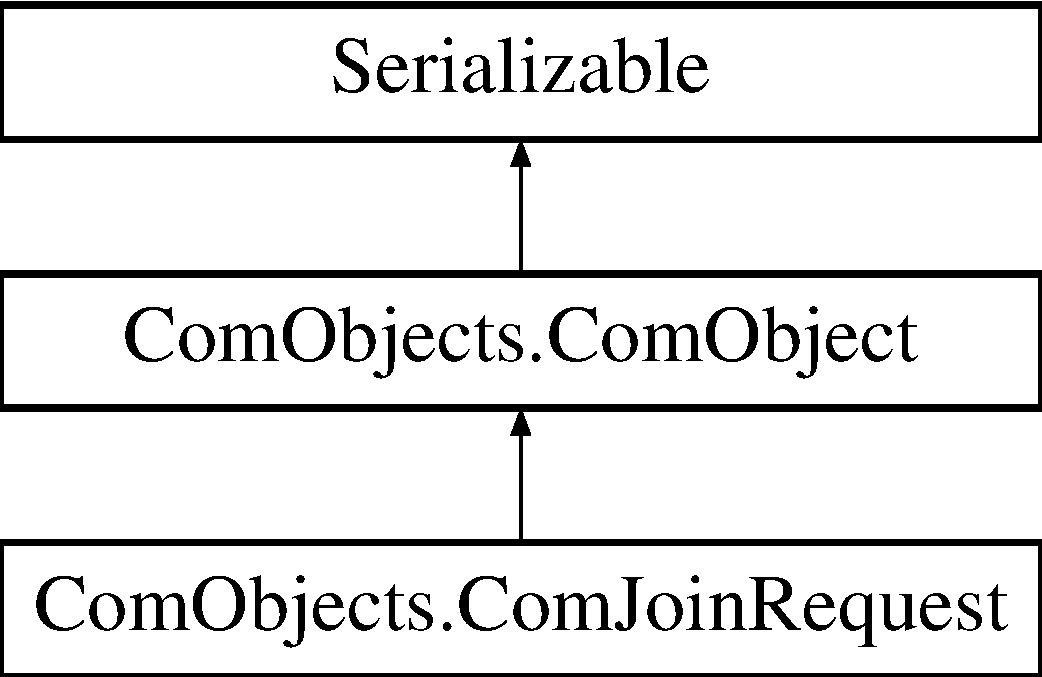
\includegraphics[height=3.000000cm]{a00025}
\end{center}
\end{figure}
\subsubsection*{Öffentliche Methoden}
\begin{DoxyCompactItemize}
\item 
\hyperlink{a00025_a3270a1088050e66b8bc6beea26c02ea1}{Com\-Join\-Request} (String game\-Master\-Name)
\item 
String \hyperlink{a00025_ab46d6375b8d4fb1e4af2b7448259dbef}{get\-Game\-Master\-Name} ()
\end{DoxyCompactItemize}


\subsubsection{Ausführliche Beschreibung}
Sie ist eine Nachricht, die an den Server gesendet wird, wenn der Spieler einem bestimmten Spiel beitreten will. Dazu enthält es den Namen des Spielleiters als String. 

\subsubsection{Beschreibung der Konstruktoren und Destruktoren}
\hypertarget{a00025_a3270a1088050e66b8bc6beea26c02ea1}{\index{Com\-Objects\-::\-Com\-Join\-Request@{Com\-Objects\-::\-Com\-Join\-Request}!Com\-Join\-Request@{Com\-Join\-Request}}
\index{Com\-Join\-Request@{Com\-Join\-Request}!ComObjects::ComJoinRequest@{Com\-Objects\-::\-Com\-Join\-Request}}
\paragraph[{Com\-Join\-Request}]{\setlength{\rightskip}{0pt plus 5cm}Com\-Objects.\-Com\-Join\-Request.\-Com\-Join\-Request (
\begin{DoxyParamCaption}
\item[{String}]{game\-Master\-Name}
\end{DoxyParamCaption}
)}}\label{a00025_a3270a1088050e66b8bc6beea26c02ea1}


Dies ist der Kontruktor für eine neue Con\-Join\-Request-\/\-Nachricht. 

Ein Spiel kann durch den eindeutigen Namen der Spielleiters identifiziert werden. 
\begin{DoxyParams}{Parameter}
{\em game\-Master\-Name} & ist der Name der Spielleiters. \\
\hline
\end{DoxyParams}


\subsubsection{Dokumentation der Elementfunktionen}
\hypertarget{a00025_ab46d6375b8d4fb1e4af2b7448259dbef}{\index{Com\-Objects\-::\-Com\-Join\-Request@{Com\-Objects\-::\-Com\-Join\-Request}!get\-Game\-Master\-Name@{get\-Game\-Master\-Name}}
\index{get\-Game\-Master\-Name@{get\-Game\-Master\-Name}!ComObjects::ComJoinRequest@{Com\-Objects\-::\-Com\-Join\-Request}}
\paragraph[{get\-Game\-Master\-Name}]{\setlength{\rightskip}{0pt plus 5cm}String Com\-Objects.\-Com\-Join\-Request.\-get\-Game\-Master\-Name (
\begin{DoxyParamCaption}
{}
\end{DoxyParamCaption}
)}}\label{a00025_ab46d6375b8d4fb1e4af2b7448259dbef}


Diese Methode gibt den Namen des Spielleiters zurück. 

Dieser ist eindeutig, so kann ein bestimmtes Spiel identifiziert werden. \begin{DoxyReturn}{Rückgabe}
den Namen des Spielleiters. 
\end{DoxyReturn}

\hypertarget{a00026}{\subsection{Com\-Objects.\-Com\-Kick\-Player\-Request Klassenreferenz}
\label{a00026}\index{Com\-Objects.\-Com\-Kick\-Player\-Request@{Com\-Objects.\-Com\-Kick\-Player\-Request}}
}
Klassendiagramm für Com\-Objects.\-Com\-Kick\-Player\-Request\-:\begin{figure}[H]
\begin{center}
\leavevmode
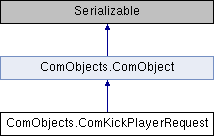
\includegraphics[height=3.000000cm]{a00026}
\end{center}
\end{figure}
\subsubsection*{Öffentliche Methoden}
\begin{DoxyCompactItemize}
\item 
\hyperlink{a00026_ac5a54122c83b74c73cfa6b1d2fc065ac}{Com\-Kick\-Player\-Request} (String player\-Name)
\item 
String \hyperlink{a00026_a75088c3733ff4556d2596fcb5ffdcd8c}{get\-Player\-Name} ()
\end{DoxyCompactItemize}


\subsubsection{Ausführliche Beschreibung}
Sie ist eine Nachricht an den Server, die angibt einen Spieler vom Spiel zu entfernen. Dazu enthält es einen String, der den Namen des Spielers enthält. 

\subsubsection{Beschreibung der Konstruktoren und Destruktoren}
\hypertarget{a00026_ac5a54122c83b74c73cfa6b1d2fc065ac}{\index{Com\-Objects\-::\-Com\-Kick\-Player\-Request@{Com\-Objects\-::\-Com\-Kick\-Player\-Request}!Com\-Kick\-Player\-Request@{Com\-Kick\-Player\-Request}}
\index{Com\-Kick\-Player\-Request@{Com\-Kick\-Player\-Request}!ComObjects::ComKickPlayerRequest@{Com\-Objects\-::\-Com\-Kick\-Player\-Request}}
\paragraph[{Com\-Kick\-Player\-Request}]{\setlength{\rightskip}{0pt plus 5cm}Com\-Objects.\-Com\-Kick\-Player\-Request.\-Com\-Kick\-Player\-Request (
\begin{DoxyParamCaption}
\item[{String}]{player\-Name}
\end{DoxyParamCaption}
)}}\label{a00026_ac5a54122c83b74c73cfa6b1d2fc065ac}


Dies ist der Kontruktor für eine neue Com\-Kick\-Player\-Request-\/\-Nachricht. 

Diese enthält den Namen des Spielers, der aus den Spiel gelöscht werden soll. 
\begin{DoxyParams}{Parameter}
{\em player\-Name} & ist der Name des Spielers. \\
\hline
\end{DoxyParams}


\subsubsection{Dokumentation der Elementfunktionen}
\hypertarget{a00026_a75088c3733ff4556d2596fcb5ffdcd8c}{\index{Com\-Objects\-::\-Com\-Kick\-Player\-Request@{Com\-Objects\-::\-Com\-Kick\-Player\-Request}!get\-Player\-Name@{get\-Player\-Name}}
\index{get\-Player\-Name@{get\-Player\-Name}!ComObjects::ComKickPlayerRequest@{Com\-Objects\-::\-Com\-Kick\-Player\-Request}}
\paragraph[{get\-Player\-Name}]{\setlength{\rightskip}{0pt plus 5cm}String Com\-Objects.\-Com\-Kick\-Player\-Request.\-get\-Player\-Name (
\begin{DoxyParamCaption}
{}
\end{DoxyParamCaption}
)}}\label{a00026_a75088c3733ff4556d2596fcb5ffdcd8c}


Diese Methode liefert den Namen des Spielers, der aus dem Spiel entfernt werden soll. 

\begin{DoxyReturn}{Rückgabe}
den Spielernamen. 
\end{DoxyReturn}

\hypertarget{a00027}{\subsection{Com\-Objects.\-Com\-Lobby\-Update\-Gamelist Klassenreferenz}
\label{a00027}\index{Com\-Objects.\-Com\-Lobby\-Update\-Gamelist@{Com\-Objects.\-Com\-Lobby\-Update\-Gamelist}}
}
Klassendiagramm für Com\-Objects.\-Com\-Lobby\-Update\-Gamelist\-:\begin{figure}[H]
\begin{center}
\leavevmode
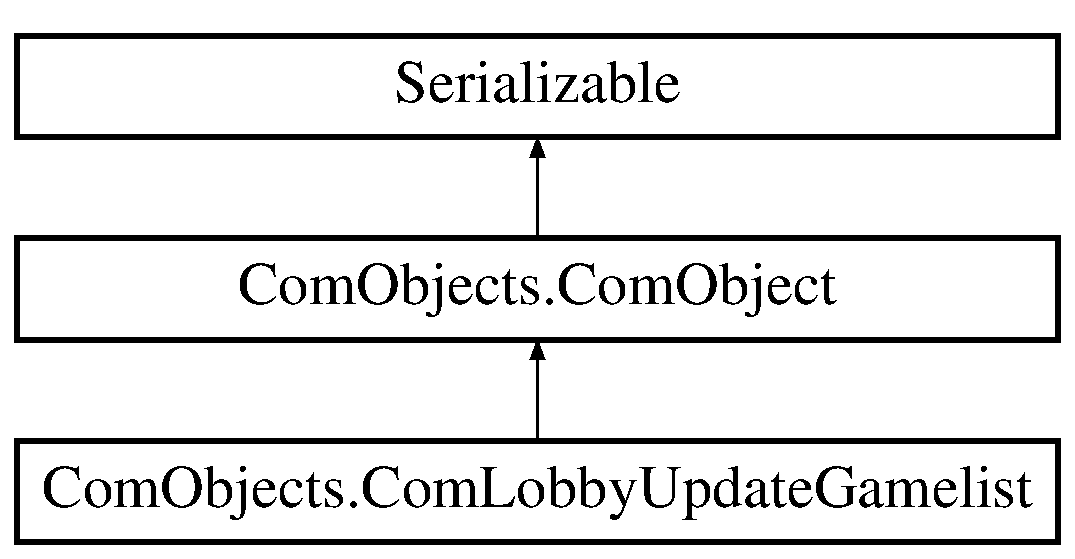
\includegraphics[height=3.000000cm]{a00027}
\end{center}
\end{figure}
\subsubsection*{Öffentliche Methoden}
\begin{DoxyCompactItemize}
\item 
\hyperlink{a00027_ab1b6eb8e3c8dccd186d1727d877a627b}{Com\-Lobby\-Update\-Gamelist} (boolean remove\-Flag, \hyperlink{a00044}{Game\-Server\-Representation} game\-Server)
\item 
boolean \hyperlink{a00027_a5aaebf8bd6d9b1a9036e1a78708638d2}{is\-Remove\-Flag} ()
\item 
\hyperlink{a00044}{Game\-Server\-Representation} \hyperlink{a00027_a0d47491338e6436c48a90f1902f25b27}{get\-Game\-Server} ()
\end{DoxyCompactItemize}


\subsubsection{Ausführliche Beschreibung}
Sie aktualisiert die Gameliste in der Lobby. Dazu enthält sie den Game\-Server und ein Remove\-Flag. 

\subsubsection{Beschreibung der Konstruktoren und Destruktoren}
\hypertarget{a00027_ab1b6eb8e3c8dccd186d1727d877a627b}{\index{Com\-Objects\-::\-Com\-Lobby\-Update\-Gamelist@{Com\-Objects\-::\-Com\-Lobby\-Update\-Gamelist}!Com\-Lobby\-Update\-Gamelist@{Com\-Lobby\-Update\-Gamelist}}
\index{Com\-Lobby\-Update\-Gamelist@{Com\-Lobby\-Update\-Gamelist}!ComObjects::ComLobbyUpdateGamelist@{Com\-Objects\-::\-Com\-Lobby\-Update\-Gamelist}}
\paragraph[{Com\-Lobby\-Update\-Gamelist}]{\setlength{\rightskip}{0pt plus 5cm}Com\-Objects.\-Com\-Lobby\-Update\-Gamelist.\-Com\-Lobby\-Update\-Gamelist (
\begin{DoxyParamCaption}
\item[{boolean}]{remove\-Flag, }
\item[{{\bf Game\-Server\-Representation}}]{game\-Server}
\end{DoxyParamCaption}
)}}\label{a00027_ab1b6eb8e3c8dccd186d1727d877a627b}


Dies ist der Kontruktor für eine neue Com\-Lobby\-Update\-Gamelist-\/\-Nachricht. 


\begin{DoxyParams}{Parameter}
{\em remove\-Flag} & zeigt an, ob das Spiel gelöscht werden soll. \\
\hline
{\em game\-Server} & ist das Spiel. \\
\hline
\end{DoxyParams}


\subsubsection{Dokumentation der Elementfunktionen}
\hypertarget{a00027_a0d47491338e6436c48a90f1902f25b27}{\index{Com\-Objects\-::\-Com\-Lobby\-Update\-Gamelist@{Com\-Objects\-::\-Com\-Lobby\-Update\-Gamelist}!get\-Game\-Server@{get\-Game\-Server}}
\index{get\-Game\-Server@{get\-Game\-Server}!ComObjects::ComLobbyUpdateGamelist@{Com\-Objects\-::\-Com\-Lobby\-Update\-Gamelist}}
\paragraph[{get\-Game\-Server}]{\setlength{\rightskip}{0pt plus 5cm}{\bf Game\-Server\-Representation} Com\-Objects.\-Com\-Lobby\-Update\-Gamelist.\-get\-Game\-Server (
\begin{DoxyParamCaption}
{}
\end{DoxyParamCaption}
)}}\label{a00027_a0d47491338e6436c48a90f1902f25b27}


Diese Methode liefert das Spiel, das geupdated werden soll. 

\begin{DoxyReturn}{Rückgabe}
das Spiel. 
\end{DoxyReturn}
\hypertarget{a00027_a5aaebf8bd6d9b1a9036e1a78708638d2}{\index{Com\-Objects\-::\-Com\-Lobby\-Update\-Gamelist@{Com\-Objects\-::\-Com\-Lobby\-Update\-Gamelist}!is\-Remove\-Flag@{is\-Remove\-Flag}}
\index{is\-Remove\-Flag@{is\-Remove\-Flag}!ComObjects::ComLobbyUpdateGamelist@{Com\-Objects\-::\-Com\-Lobby\-Update\-Gamelist}}
\paragraph[{is\-Remove\-Flag}]{\setlength{\rightskip}{0pt plus 5cm}boolean Com\-Objects.\-Com\-Lobby\-Update\-Gamelist.\-is\-Remove\-Flag (
\begin{DoxyParamCaption}
{}
\end{DoxyParamCaption}
)}}\label{a00027_a5aaebf8bd6d9b1a9036e1a78708638d2}


Diese Methode liefert, ob ein Spiel gelöscht werden soll oder nicht. 

\begin{DoxyReturn}{Rückgabe}
ob das Spiel gelöscht wird. 
\end{DoxyReturn}

\hypertarget{a00028}{\subsection{Com\-Client\-Quit Klassenreferenz}
\label{a00028}\index{Com\-Client\-Quit@{Com\-Client\-Quit}}
}


Abgeleitet von \hyperlink{a00037}{Com\-Object} und Serializable.

\subsubsection*{Öffentliche Methoden}
\begin{DoxyCompactItemize}
\item 
\hypertarget{a00028_a52307476eb55f9bf5ab7174c2b113676}{\hyperlink{a00028_a52307476eb55f9bf5ab7174c2b113676}{Com\-Client\-Quit} ()}\label{a00028_a52307476eb55f9bf5ab7174c2b113676}

\item 
void \hyperlink{a00028_a758d7005755a181717f238f714d87dd2}{process} (\hyperlink{a00003}{Client\-Model} model)
\item 
void \hyperlink{a00028_ac67b5ce3ec03d48ef1e6caad6e49c902}{process} (\hyperlink{a00076}{Player} player, \hyperlink{a00077}{Server} server)
\end{DoxyCompactItemize}


\subsubsection{Ausführliche Beschreibung}
Diese Klasse ist ein spezielles Kommunikations-\/\-Objekt. Die Nachricht wird verschickt, wenn der Spieler ein Fenster schließt. 

\subsubsection{Dokumentation der Elementfunktionen}
\hypertarget{a00028_a758d7005755a181717f238f714d87dd2}{\index{Com\-Objects\-::\-Com\-Client\-Quit@{Com\-Objects\-::\-Com\-Client\-Quit}!process@{process}}
\index{process@{process}!ComObjects::ComClientQuit@{Com\-Objects\-::\-Com\-Client\-Quit}}
\paragraph[{process}]{\setlength{\rightskip}{0pt plus 5cm}void process (
\begin{DoxyParamCaption}
\item[{{\bf Client\-Model}}]{model}
\end{DoxyParamCaption}
)}}\label{a00028_a758d7005755a181717f238f714d87dd2}


Diese Methode ist noetig, damit der Client\-Listener\-Thread entscheiden kann welche Message das Object enthaelt und wie diese verarbeitet werden soll. 


\begin{DoxyParams}{Parameter}
{\em model} & ist das Client\-Model, welches übergeben wird, damit die ueberladene Methode richtig gewaehlt wird. \\
\hline
\end{DoxyParams}


Implementiert \hyperlink{a00037_a758d7005755a181717f238f714d87dd2}{Com\-Object}.

\hypertarget{a00028_ac67b5ce3ec03d48ef1e6caad6e49c902}{\index{Com\-Objects\-::\-Com\-Client\-Quit@{Com\-Objects\-::\-Com\-Client\-Quit}!process@{process}}
\index{process@{process}!ComObjects::ComClientQuit@{Com\-Objects\-::\-Com\-Client\-Quit}}
\paragraph[{process}]{\setlength{\rightskip}{0pt plus 5cm}void process (
\begin{DoxyParamCaption}
\item[{{\bf Player}}]{player, }
\item[{{\bf Server}}]{server}
\end{DoxyParamCaption}
)}}\label{a00028_ac67b5ce3ec03d48ef1e6caad6e49c902}


Diese Methode ist noetig, damit der Thread Player entscheiden kann welche Message das Object enthaelt und wie diese verarbeitet werden soll. 


\begin{DoxyParams}{Parameter}
{\em player} & Der Client welcher den Aufruf startet. \\
\hline
{\em server} & Der Server an den sich das Com\-Objekt weitergibt. \\
\hline
\end{DoxyParams}


Implementiert \hyperlink{a00037_ac67b5ce3ec03d48ef1e6caad6e49c902}{Com\-Object}.


\hypertarget{a00029}{\subsection{Com\-Objects.\-Com\-Object Klassenreferenz}
\label{a00029}\index{Com\-Objects.\-Com\-Object@{Com\-Objects.\-Com\-Object}}
}
Klassendiagramm für Com\-Objects.\-Com\-Object\-:\begin{figure}[H]
\begin{center}
\leavevmode
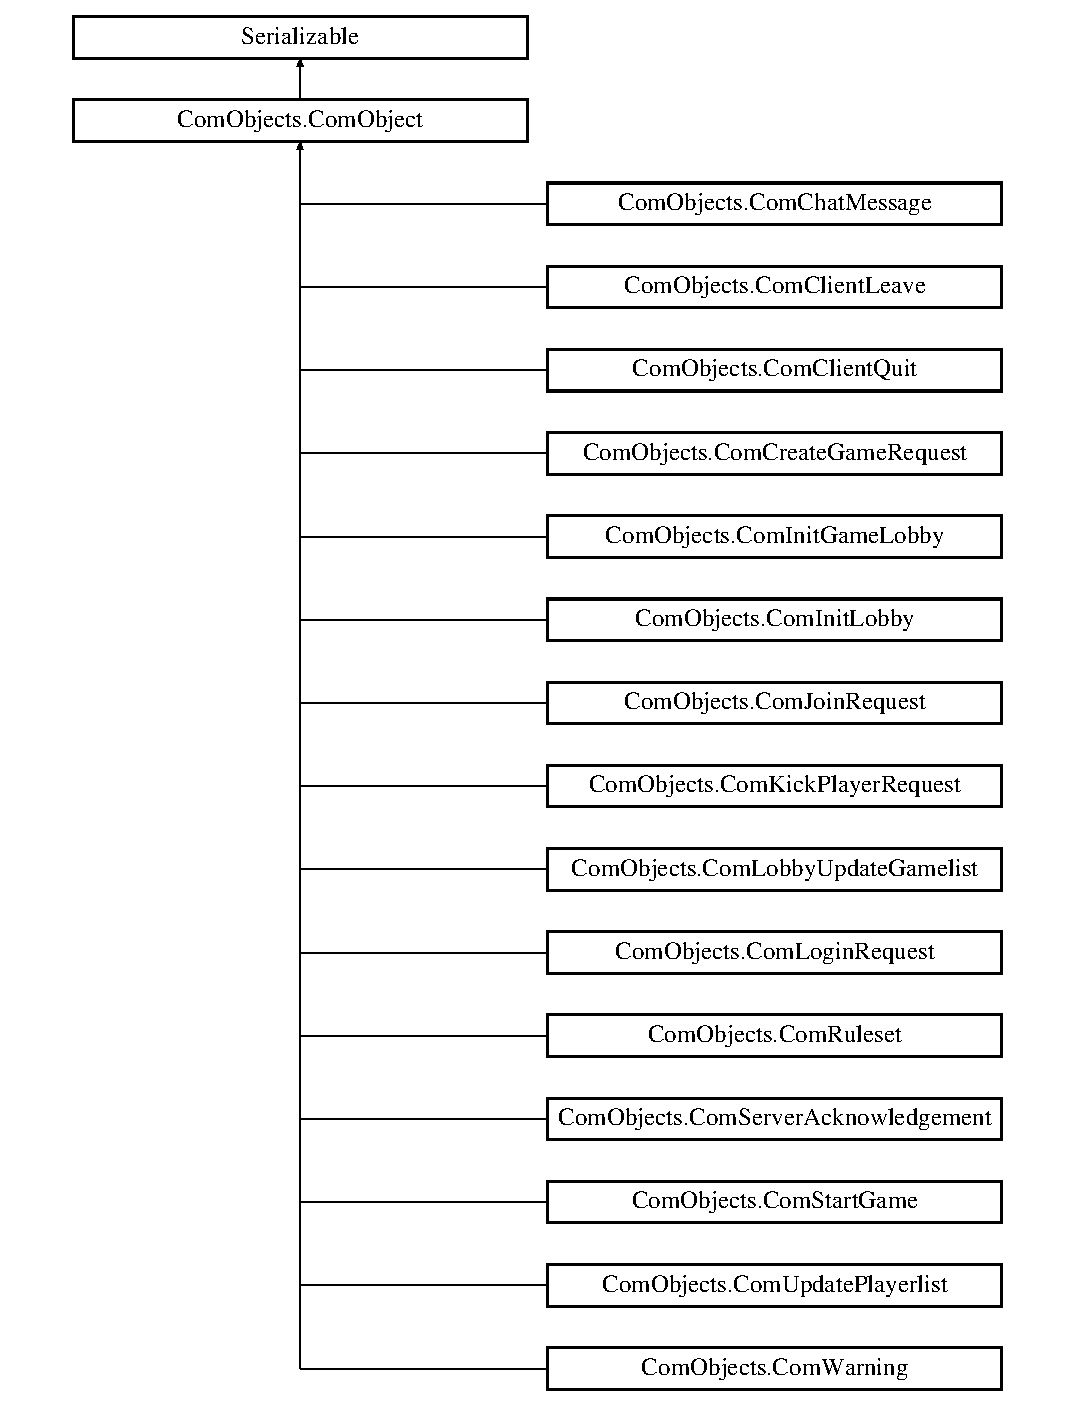
\includegraphics[height=12.000000cm]{a00029}
\end{center}
\end{figure}

\hypertarget{a00030}{\subsection{Com\-Objects.\-Com\-Ruleset Klassenreferenz}
\label{a00030}\index{Com\-Objects.\-Com\-Ruleset@{Com\-Objects.\-Com\-Ruleset}}
}
Klassendiagramm für Com\-Objects.\-Com\-Ruleset\-:\begin{figure}[H]
\begin{center}
\leavevmode
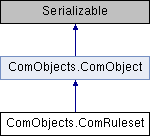
\includegraphics[height=3.000000cm]{a00030}
\end{center}
\end{figure}
\subsubsection*{Öffentliche Methoden}
\begin{DoxyCompactItemize}
\item 
\hyperlink{a00030_a980db8cc8a90bf9fe42535fd4147eb53}{Com\-Ruleset} (\hyperlink{a00075}{Ruleset\-Message} ruleset\-Message)
\item 
\hyperlink{a00075}{Ruleset\-Message} \hyperlink{a00030_a21ffb1a0df071d6e0e5d1f8e16e847b2}{get\-Ruleset\-Message} ()
\end{DoxyCompactItemize}


\subsubsection{Ausführliche Beschreibung}
Sie ist die grundlegende Nachricht eines Regelwerkaufrufes und enthält eine verfeinerte Nachricht mit weiteren Informationen, die \hyperlink{a00075}{Ruleset\-Message}. 

\subsubsection{Beschreibung der Konstruktoren und Destruktoren}
\hypertarget{a00030_a980db8cc8a90bf9fe42535fd4147eb53}{\index{Com\-Objects\-::\-Com\-Ruleset@{Com\-Objects\-::\-Com\-Ruleset}!Com\-Ruleset@{Com\-Ruleset}}
\index{Com\-Ruleset@{Com\-Ruleset}!ComObjects::ComRuleset@{Com\-Objects\-::\-Com\-Ruleset}}
\paragraph[{Com\-Ruleset}]{\setlength{\rightskip}{0pt plus 5cm}Com\-Objects.\-Com\-Ruleset.\-Com\-Ruleset (
\begin{DoxyParamCaption}
\item[{{\bf Ruleset\-Message}}]{ruleset\-Message}
\end{DoxyParamCaption}
)}}\label{a00030_a980db8cc8a90bf9fe42535fd4147eb53}


Dies ist der Kontruktor für eine neue Com\-Result-\/\-Nachricht. 


\begin{DoxyParams}{Parameter}
{\em ruleset\-Message} & ist eine Nachricht, die ans Ruleset gesendet werden soll. \\
\hline
\end{DoxyParams}


\subsubsection{Dokumentation der Elementfunktionen}
\hypertarget{a00030_a21ffb1a0df071d6e0e5d1f8e16e847b2}{\index{Com\-Objects\-::\-Com\-Ruleset@{Com\-Objects\-::\-Com\-Ruleset}!get\-Ruleset\-Message@{get\-Ruleset\-Message}}
\index{get\-Ruleset\-Message@{get\-Ruleset\-Message}!ComObjects::ComRuleset@{Com\-Objects\-::\-Com\-Ruleset}}
\paragraph[{get\-Ruleset\-Message}]{\setlength{\rightskip}{0pt plus 5cm}{\bf Ruleset\-Message} Com\-Objects.\-Com\-Ruleset.\-get\-Ruleset\-Message (
\begin{DoxyParamCaption}
{}
\end{DoxyParamCaption}
)}}\label{a00030_a21ffb1a0df071d6e0e5d1f8e16e847b2}


Diese Methode gibt die Nachricht zurück, die ans Ruleset gesendet werden soll. 

\begin{DoxyReturn}{Rückgabe}
die Nachricht. 
\end{DoxyReturn}

\hypertarget{a00031}{\subsection{Com\-Init\-Game\-Lobby Klassenreferenz}
\label{a00031}\index{Com\-Init\-Game\-Lobby@{Com\-Init\-Game\-Lobby}}
}


Abgeleitet von \hyperlink{a00037}{Com\-Object} und Serializable.

\subsubsection*{Öffentliche Methoden}
\begin{DoxyCompactItemize}
\item 
\hyperlink{a00031_a6bd6086583fdd9b6fc25d1aabb9f1312}{Com\-Init\-Game\-Lobby} (List$<$ String $>$ player\-List)
\item 
List$<$ String $>$ \hyperlink{a00031_a806a371665b36cee69f0a49625a8c20d}{get\-Player\-List} ()
\item 
void \hyperlink{a00031_a758d7005755a181717f238f714d87dd2}{process} (\hyperlink{a00003}{Client\-Model} model)
\item 
void \hyperlink{a00031_ac67b5ce3ec03d48ef1e6caad6e49c902}{process} (\hyperlink{a00076}{Player} player, \hyperlink{a00077}{Server} server)
\end{DoxyCompactItemize}
\subsubsection*{Private Attribute}
\begin{DoxyCompactItemize}
\item 
\hypertarget{a00031_a2a62caed4423183b9e69deb6560b136f}{List$<$ String $>$ {\bfseries player\-List}}\label{a00031_a2a62caed4423183b9e69deb6560b136f}

\end{DoxyCompactItemize}


\subsubsection{Ausführliche Beschreibung}
Diese Klasse ist ein spezielles Kommunikations-\/\-Objekt. Sie liefert die Liste der Spieler, die sich bereits beim Betreten des Wartefensters darin befinden. 

\subsubsection{Beschreibung der Konstruktoren und Destruktoren}
\hypertarget{a00031_a6bd6086583fdd9b6fc25d1aabb9f1312}{\index{Com\-Objects\-::\-Com\-Init\-Game\-Lobby@{Com\-Objects\-::\-Com\-Init\-Game\-Lobby}!Com\-Init\-Game\-Lobby@{Com\-Init\-Game\-Lobby}}
\index{Com\-Init\-Game\-Lobby@{Com\-Init\-Game\-Lobby}!ComObjects::ComInitGameLobby@{Com\-Objects\-::\-Com\-Init\-Game\-Lobby}}
\paragraph[{Com\-Init\-Game\-Lobby}]{\setlength{\rightskip}{0pt plus 5cm}{\bf Com\-Init\-Game\-Lobby} (
\begin{DoxyParamCaption}
\item[{List$<$ String $>$}]{player\-List}
\end{DoxyParamCaption}
)}}\label{a00031_a6bd6086583fdd9b6fc25d1aabb9f1312}


Dies ist der Kontruktor fuer eine neue Com\-Init\-Game\-Lobby-\/\-Nachricht. 


\begin{DoxyParams}{Parameter}
{\em player\-List} & ist die Liste aller Player, die sich im Wartefenster befinden. \\
\hline
\end{DoxyParams}


\subsubsection{Dokumentation der Elementfunktionen}
\hypertarget{a00031_a806a371665b36cee69f0a49625a8c20d}{\index{Com\-Objects\-::\-Com\-Init\-Game\-Lobby@{Com\-Objects\-::\-Com\-Init\-Game\-Lobby}!get\-Player\-List@{get\-Player\-List}}
\index{get\-Player\-List@{get\-Player\-List}!ComObjects::ComInitGameLobby@{Com\-Objects\-::\-Com\-Init\-Game\-Lobby}}
\paragraph[{get\-Player\-List}]{\setlength{\rightskip}{0pt plus 5cm}List$<$String$>$ get\-Player\-List (
\begin{DoxyParamCaption}
{}
\end{DoxyParamCaption}
)}}\label{a00031_a806a371665b36cee69f0a49625a8c20d}


Diese Methode liefert die Liste der Player, die sich beim Hinzufuegen eines weiteren Spielers bereits im Wartefenster befinden. 

\begin{DoxyReturn}{Rückgabe}
die Liste der Spieler, die im Wartefenster sind. 
\end{DoxyReturn}
\hypertarget{a00031_a758d7005755a181717f238f714d87dd2}{\index{Com\-Objects\-::\-Com\-Init\-Game\-Lobby@{Com\-Objects\-::\-Com\-Init\-Game\-Lobby}!process@{process}}
\index{process@{process}!ComObjects::ComInitGameLobby@{Com\-Objects\-::\-Com\-Init\-Game\-Lobby}}
\paragraph[{process}]{\setlength{\rightskip}{0pt plus 5cm}void process (
\begin{DoxyParamCaption}
\item[{{\bf Client\-Model}}]{model}
\end{DoxyParamCaption}
)}}\label{a00031_a758d7005755a181717f238f714d87dd2}


Diese Methode ist noetig, damit der Client\-Listener\-Thread entscheiden kann welche Message das Object enthaelt und wie diese verarbeitet werden soll. 


\begin{DoxyParams}{Parameter}
{\em model} & ist das Client\-Model, welches übergeben wird, damit die ueberladene Methode richtig gewaehlt wird. \\
\hline
\end{DoxyParams}


Implementiert \hyperlink{a00037_a758d7005755a181717f238f714d87dd2}{Com\-Object}.

\hypertarget{a00031_ac67b5ce3ec03d48ef1e6caad6e49c902}{\index{Com\-Objects\-::\-Com\-Init\-Game\-Lobby@{Com\-Objects\-::\-Com\-Init\-Game\-Lobby}!process@{process}}
\index{process@{process}!ComObjects::ComInitGameLobby@{Com\-Objects\-::\-Com\-Init\-Game\-Lobby}}
\paragraph[{process}]{\setlength{\rightskip}{0pt plus 5cm}void process (
\begin{DoxyParamCaption}
\item[{{\bf Player}}]{player, }
\item[{{\bf Server}}]{server}
\end{DoxyParamCaption}
)}}\label{a00031_ac67b5ce3ec03d48ef1e6caad6e49c902}


Diese Methode ist noetig, damit der Thread Player entscheiden kann welche Message das Object enthaelt und wie diese verarbeitet werden soll. 


\begin{DoxyParams}{Parameter}
{\em player} & Der Client welcher den Aufruf startet. \\
\hline
{\em server} & Der Server an den sich das Com\-Objekt weitergibt. \\
\hline
\end{DoxyParams}


Implementiert \hyperlink{a00037_ac67b5ce3ec03d48ef1e6caad6e49c902}{Com\-Object}.


\hypertarget{a00032}{\subsection{Com\-Objects.\-Com\-Start\-Game Klassenreferenz}
\label{a00032}\index{Com\-Objects.\-Com\-Start\-Game@{Com\-Objects.\-Com\-Start\-Game}}
}
Klassendiagramm für Com\-Objects.\-Com\-Start\-Game\-:\begin{figure}[H]
\begin{center}
\leavevmode
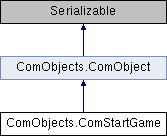
\includegraphics[height=3.000000cm]{a00032}
\end{center}
\end{figure}


\subsubsection{Ausführliche Beschreibung}
Sie wird versendet, wenn ein Spiel gestartet werden soll. 
\hypertarget{a00033}{\subsection{Com\-Join\-Request Klassenreferenz}
\label{a00033}\index{Com\-Join\-Request@{Com\-Join\-Request}}
}


Abgeleitet von \hyperlink{a00037}{Com\-Object} und Serializable.

\subsubsection*{Öffentliche Methoden}
\begin{DoxyCompactItemize}
\item 
\hyperlink{a00033_a65c627c4c6752c8b94d729645b03846f}{Com\-Join\-Request} (String \hyperlink{a00033_ad3f74f58e5b41a74c02e21e0407280b8}{game\-Master\-Name}, String password)
\item 
String \hyperlink{a00033_a3acba35c72b8d4dcf49579142910672f}{get\-Game\-Master\-Name} ()
\item 
void \hyperlink{a00033_a758d7005755a181717f238f714d87dd2}{process} (\hyperlink{a00003}{Client\-Model} model)
\item 
void \hyperlink{a00033_ac67b5ce3ec03d48ef1e6caad6e49c902}{process} (\hyperlink{a00076}{Player} player, \hyperlink{a00077}{Server} server)
\end{DoxyCompactItemize}
\subsubsection*{Private Attribute}
\begin{DoxyCompactItemize}
\item 
String \hyperlink{a00033_ad3f74f58e5b41a74c02e21e0407280b8}{game\-Master\-Name}
\item 
\hypertarget{a00033_acbd76b816d055b7a642c219fd9751020}{String {\bfseries password}}\label{a00033_acbd76b816d055b7a642c219fd9751020}

\end{DoxyCompactItemize}


\subsubsection{Ausführliche Beschreibung}
Diese Klasse ist ein spezielles Kommunikations-\/\-Objekt. Sie ist eine Nachricht, die an den Server gesendet wird, wenn der Spieler einem bestimmten Spiel beitreten will. Dazu enthaelt sie den Namen des Spielleiters als String und ein Passwort, falls dieses von Spielleiter gesetzt wurde. 

\subsubsection{Beschreibung der Konstruktoren und Destruktoren}
\hypertarget{a00033_a65c627c4c6752c8b94d729645b03846f}{\index{Com\-Objects\-::\-Com\-Join\-Request@{Com\-Objects\-::\-Com\-Join\-Request}!Com\-Join\-Request@{Com\-Join\-Request}}
\index{Com\-Join\-Request@{Com\-Join\-Request}!ComObjects::ComJoinRequest@{Com\-Objects\-::\-Com\-Join\-Request}}
\paragraph[{Com\-Join\-Request}]{\setlength{\rightskip}{0pt plus 5cm}{\bf Com\-Join\-Request} (
\begin{DoxyParamCaption}
\item[{String}]{game\-Master\-Name, }
\item[{String}]{password}
\end{DoxyParamCaption}
)}}\label{a00033_a65c627c4c6752c8b94d729645b03846f}


Dies ist der Kontruktor fuer eine neue Con\-Join\-Request-\/\-Nachricht. 

Ein Spiel kann durch den eindeutigen Namen der Spielleiters identifiziert werden. 
\begin{DoxyParams}{Parameter}
{\em game\-Master\-Name} & ist der Name der Spielleiters. \\
\hline
{\em password} & fuer das Spiel. \\
\hline
\end{DoxyParams}


Benutzt Com\-Join\-Request.\-game\-Master\-Name.



\subsubsection{Dokumentation der Elementfunktionen}
\hypertarget{a00033_a3acba35c72b8d4dcf49579142910672f}{\index{Com\-Objects\-::\-Com\-Join\-Request@{Com\-Objects\-::\-Com\-Join\-Request}!get\-Game\-Master\-Name@{get\-Game\-Master\-Name}}
\index{get\-Game\-Master\-Name@{get\-Game\-Master\-Name}!ComObjects::ComJoinRequest@{Com\-Objects\-::\-Com\-Join\-Request}}
\paragraph[{get\-Game\-Master\-Name}]{\setlength{\rightskip}{0pt plus 5cm}String get\-Game\-Master\-Name (
\begin{DoxyParamCaption}
{}
\end{DoxyParamCaption}
)}}\label{a00033_a3acba35c72b8d4dcf49579142910672f}


Diese Methode gibt den Namen des Spielleiters zurueck. 

Dieser ist eindeutig, so kann ein bestimmtes Spiel identifiziert werden. \begin{DoxyReturn}{Rückgabe}
der Name des Spielleiters. 
\end{DoxyReturn}


Benutzt Com\-Join\-Request.\-game\-Master\-Name.

\hypertarget{a00033_a758d7005755a181717f238f714d87dd2}{\index{Com\-Objects\-::\-Com\-Join\-Request@{Com\-Objects\-::\-Com\-Join\-Request}!process@{process}}
\index{process@{process}!ComObjects::ComJoinRequest@{Com\-Objects\-::\-Com\-Join\-Request}}
\paragraph[{process}]{\setlength{\rightskip}{0pt plus 5cm}void process (
\begin{DoxyParamCaption}
\item[{{\bf Client\-Model}}]{model}
\end{DoxyParamCaption}
)}}\label{a00033_a758d7005755a181717f238f714d87dd2}


Diese Methode ist noetig, damit der Client\-Listener\-Thread entscheiden kann welche Message das Object enthaelt und wie diese verarbeitet werden soll. 


\begin{DoxyParams}{Parameter}
{\em model} & ist das Client\-Model, welches übergeben wird, damit die ueberladene Methode richtig gewaehlt wird. \\
\hline
\end{DoxyParams}


Implementiert \hyperlink{a00037_a758d7005755a181717f238f714d87dd2}{Com\-Object}.

\hypertarget{a00033_ac67b5ce3ec03d48ef1e6caad6e49c902}{\index{Com\-Objects\-::\-Com\-Join\-Request@{Com\-Objects\-::\-Com\-Join\-Request}!process@{process}}
\index{process@{process}!ComObjects::ComJoinRequest@{Com\-Objects\-::\-Com\-Join\-Request}}
\paragraph[{process}]{\setlength{\rightskip}{0pt plus 5cm}void process (
\begin{DoxyParamCaption}
\item[{{\bf Player}}]{player, }
\item[{{\bf Server}}]{server}
\end{DoxyParamCaption}
)}}\label{a00033_ac67b5ce3ec03d48ef1e6caad6e49c902}


Diese Methode ist noetig, damit der Thread Player entscheiden kann welche Message das Object enthaelt und wie diese verarbeitet werden soll. 


\begin{DoxyParams}{Parameter}
{\em player} & Der Client welcher den Aufruf startet. \\
\hline
{\em server} & Der Server an den sich das Com\-Objekt weitergibt. \\
\hline
\end{DoxyParams}


Implementiert \hyperlink{a00037_ac67b5ce3ec03d48ef1e6caad6e49c902}{Com\-Object}.



\subsubsection{Dokumentation der Datenelemente}
\hypertarget{a00033_ad3f74f58e5b41a74c02e21e0407280b8}{\index{Com\-Objects\-::\-Com\-Join\-Request@{Com\-Objects\-::\-Com\-Join\-Request}!game\-Master\-Name@{game\-Master\-Name}}
\index{game\-Master\-Name@{game\-Master\-Name}!ComObjects::ComJoinRequest@{Com\-Objects\-::\-Com\-Join\-Request}}
\paragraph[{game\-Master\-Name}]{\setlength{\rightskip}{0pt plus 5cm}String game\-Master\-Name\hspace{0.3cm}{\ttfamily [private]}}}\label{a00033_ad3f74f58e5b41a74c02e21e0407280b8}


Der Name der Spielleiters muss enthalten sein um ein Spiel zuzuornen. 

Der Spielname ist nicht eindeutig, aber der Spielleiter schon. Somit kann jedes Spiel mit Hilfe des Spielleiters identifiziert werden. 

Wird benutzt von Com\-Join\-Request.\-Com\-Join\-Request() und Com\-Join\-Request.\-get\-Game\-Master\-Name().


\hypertarget{a00034}{\subsection{Com\-Kick\-Player\-Request Klassenreferenz}
\label{a00034}\index{Com\-Kick\-Player\-Request@{Com\-Kick\-Player\-Request}}
}


Abgeleitet von \hyperlink{a00037}{Com\-Object} und Serializable.

\subsubsection*{Öffentliche Methoden}
\begin{DoxyCompactItemize}
\item 
\hyperlink{a00034_ae62e08a885d902a978f355560928a796}{Com\-Kick\-Player\-Request} (String \hyperlink{a00034_a12adf3f64463f614eb3af6dd82414e0a}{player\-Name})
\item 
String \hyperlink{a00034_a8cd2886758be9855ae14404540d4873d}{get\-Player\-Name} ()
\item 
void \hyperlink{a00034_a758d7005755a181717f238f714d87dd2}{process} (\hyperlink{a00003}{Client\-Model} model)
\item 
void \hyperlink{a00034_ac67b5ce3ec03d48ef1e6caad6e49c902}{process} (\hyperlink{a00076}{Player} player, \hyperlink{a00077}{Server} server)
\end{DoxyCompactItemize}
\subsubsection*{Private Attribute}
\begin{DoxyCompactItemize}
\item 
\hypertarget{a00034_a12adf3f64463f614eb3af6dd82414e0a}{String \hyperlink{a00034_a12adf3f64463f614eb3af6dd82414e0a}{player\-Name}}\label{a00034_a12adf3f64463f614eb3af6dd82414e0a}

\end{DoxyCompactItemize}


\subsubsection{Ausführliche Beschreibung}
Diese Klasse ist ein spezielles Kommunikations-\/\-Objekt. Sie ist eine Nachricht an den Server, die angibt einen Spieler vom Spiel zu entfernen. Dazu enthaelt sie einen String, der den Namen des Spielers enthaelt. 

\subsubsection{Beschreibung der Konstruktoren und Destruktoren}
\hypertarget{a00034_ae62e08a885d902a978f355560928a796}{\index{Com\-Objects\-::\-Com\-Kick\-Player\-Request@{Com\-Objects\-::\-Com\-Kick\-Player\-Request}!Com\-Kick\-Player\-Request@{Com\-Kick\-Player\-Request}}
\index{Com\-Kick\-Player\-Request@{Com\-Kick\-Player\-Request}!ComObjects::ComKickPlayerRequest@{Com\-Objects\-::\-Com\-Kick\-Player\-Request}}
\paragraph[{Com\-Kick\-Player\-Request}]{\setlength{\rightskip}{0pt plus 5cm}{\bf Com\-Kick\-Player\-Request} (
\begin{DoxyParamCaption}
\item[{String}]{player\-Name}
\end{DoxyParamCaption}
)}}\label{a00034_ae62e08a885d902a978f355560928a796}


Dies ist der Kontruktor fuer eine neue Com\-Kick\-Player\-Request-\/\-Nachricht. 

Diese enthaelt den Namen des Spielers, der aus den Spiel geloescht werden soll. 
\begin{DoxyParams}{Parameter}
{\em player\-Name} & ist der Name des Spielers. \\
\hline
\end{DoxyParams}


Benutzt Com\-Kick\-Player\-Request.\-player\-Name.



\subsubsection{Dokumentation der Elementfunktionen}
\hypertarget{a00034_a8cd2886758be9855ae14404540d4873d}{\index{Com\-Objects\-::\-Com\-Kick\-Player\-Request@{Com\-Objects\-::\-Com\-Kick\-Player\-Request}!get\-Player\-Name@{get\-Player\-Name}}
\index{get\-Player\-Name@{get\-Player\-Name}!ComObjects::ComKickPlayerRequest@{Com\-Objects\-::\-Com\-Kick\-Player\-Request}}
\paragraph[{get\-Player\-Name}]{\setlength{\rightskip}{0pt plus 5cm}String get\-Player\-Name (
\begin{DoxyParamCaption}
{}
\end{DoxyParamCaption}
)}}\label{a00034_a8cd2886758be9855ae14404540d4873d}


Diese Methode liefert den Namen des Spielers, der aus dem Spiel entfernt werden soll. 

\begin{DoxyReturn}{Rückgabe}
den Spielernamen. 
\end{DoxyReturn}


Benutzt Com\-Kick\-Player\-Request.\-player\-Name.

\hypertarget{a00034_a758d7005755a181717f238f714d87dd2}{\index{Com\-Objects\-::\-Com\-Kick\-Player\-Request@{Com\-Objects\-::\-Com\-Kick\-Player\-Request}!process@{process}}
\index{process@{process}!ComObjects::ComKickPlayerRequest@{Com\-Objects\-::\-Com\-Kick\-Player\-Request}}
\paragraph[{process}]{\setlength{\rightskip}{0pt plus 5cm}void process (
\begin{DoxyParamCaption}
\item[{{\bf Client\-Model}}]{model}
\end{DoxyParamCaption}
)}}\label{a00034_a758d7005755a181717f238f714d87dd2}


Diese Methode ist noetig, damit der Client\-Listener\-Thread entscheiden kann welche Message das Object enthaelt und wie diese verarbeitet werden soll. 


\begin{DoxyParams}{Parameter}
{\em model} & ist das Client\-Model, welches übergeben wird, damit die ueberladene Methode richtig gewaehlt wird. \\
\hline
\end{DoxyParams}


Implementiert \hyperlink{a00037_a758d7005755a181717f238f714d87dd2}{Com\-Object}.

\hypertarget{a00034_ac67b5ce3ec03d48ef1e6caad6e49c902}{\index{Com\-Objects\-::\-Com\-Kick\-Player\-Request@{Com\-Objects\-::\-Com\-Kick\-Player\-Request}!process@{process}}
\index{process@{process}!ComObjects::ComKickPlayerRequest@{Com\-Objects\-::\-Com\-Kick\-Player\-Request}}
\paragraph[{process}]{\setlength{\rightskip}{0pt plus 5cm}void process (
\begin{DoxyParamCaption}
\item[{{\bf Player}}]{player, }
\item[{{\bf Server}}]{server}
\end{DoxyParamCaption}
)}}\label{a00034_ac67b5ce3ec03d48ef1e6caad6e49c902}


Diese Methode ist noetig, damit der Thread Player entscheiden kann welche Message das Object enthaelt und wie diese verarbeitet werden soll. 


\begin{DoxyParams}{Parameter}
{\em player} & Der Client welcher den Aufruf startet. \\
\hline
{\em server} & Der Server an den sich das Com\-Objekt weitergibt. \\
\hline
\end{DoxyParams}


Implementiert \hyperlink{a00037_ac67b5ce3ec03d48ef1e6caad6e49c902}{Com\-Object}.


\hypertarget{a00035}{\subsection{Client.\-View.\-Create\-Game Klassenreferenz}
\label{a00035}\index{Client.\-View.\-Create\-Game@{Client.\-View.\-Create\-Game}}
}
Klassendiagramm für Client.\-View.\-Create\-Game\-:\begin{figure}[H]
\begin{center}
\leavevmode
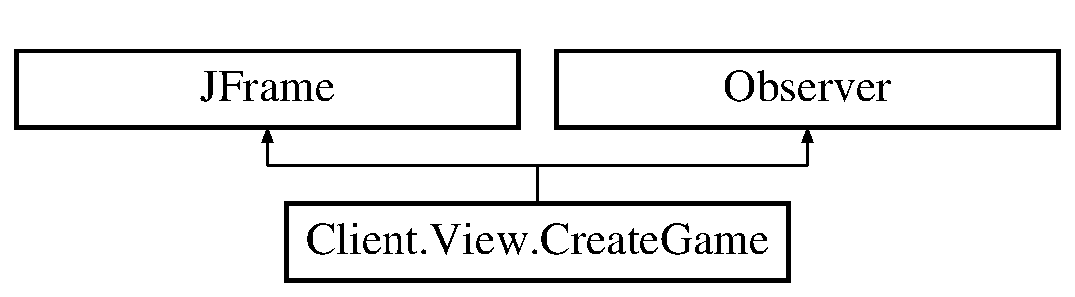
\includegraphics[height=2.000000cm]{a00035}
\end{center}
\end{figure}
\subsubsection*{Öffentliche Methoden}
\begin{DoxyCompactItemize}
\item 
\hyperlink{a00035_af35c00524077f6cda2d0c0397ce032a5}{Create\-Game} ()  throws I\-O\-Exception 
\item 
void \hyperlink{a00035_a0c95e9377fb0c48543c65d7c39c26fc1}{update} (Observable o, Object arg)
\end{DoxyCompactItemize}


\subsubsection{Ausführliche Beschreibung}
Es bietet alle Komponenten, um ein Regelwerk zu w�hlen, einen Spielnamen festzulegen und das Spiel durch ein Passwort zu sch�tzen. In der Spielerstellung wird ein Titelbild des ausgew�hlten Spiels und eine kurze Beschreibung angezeigt. �ber 'Leave' kehrt der Spieler in die \hyperlink{a00053}{Lobby} zur�ck und mit 'Create' wird das Spiel erstellt.

\begin{DoxyAuthor}{Autor}
M4nkey 
\end{DoxyAuthor}


\subsubsection{Beschreibung der Konstruktoren und Destruktoren}
\hypertarget{a00035_af35c00524077f6cda2d0c0397ce032a5}{\index{Client\-::\-View\-::\-Create\-Game@{Client\-::\-View\-::\-Create\-Game}!Create\-Game@{Create\-Game}}
\index{Create\-Game@{Create\-Game}!Client::View::CreateGame@{Client\-::\-View\-::\-Create\-Game}}
\paragraph[{Create\-Game}]{\setlength{\rightskip}{0pt plus 5cm}Client.\-View.\-Create\-Game.\-Create\-Game (
\begin{DoxyParamCaption}
{}
\end{DoxyParamCaption}
) throws I\-O\-Exception}}\label{a00035_af35c00524077f6cda2d0c0397ce032a5}


Erstellt das \hyperlink{a00035}{Create\-Game} Fenster. 


\begin{DoxyExceptions}{Ausnahmebehandlung}
{\em I\-O\-Exception} & \\
\hline
\end{DoxyExceptions}


\subsubsection{Dokumentation der Elementfunktionen}
\hypertarget{a00035_a0c95e9377fb0c48543c65d7c39c26fc1}{\index{Client\-::\-View\-::\-Create\-Game@{Client\-::\-View\-::\-Create\-Game}!update@{update}}
\index{update@{update}!Client::View::CreateGame@{Client\-::\-View\-::\-Create\-Game}}
\paragraph[{update}]{\setlength{\rightskip}{0pt plus 5cm}void Client.\-View.\-Create\-Game.\-update (
\begin{DoxyParamCaption}
\item[{Observable}]{o, }
\item[{Object}]{arg}
\end{DoxyParamCaption}
)}}\label{a00035_a0c95e9377fb0c48543c65d7c39c26fc1}


Wird durch notify() im \hyperlink{a00013}{Client\-Model} aufgerufen. 

Je nach dem in arg �bergebenen Befehl wird ein Update des Fensters ausgef�hrt oder eine Fehlermeldung angezeigt.


\begin{DoxyParams}{Parameter}
{\em o} & erwartet ein Objekt von der Klasse \hyperlink{a00013}{Client\-Model} \\
\hline
{\em arg} & erwartet\-: window\-Change\-Acknowledged, window\-Change\-Denied \\
\hline
\end{DoxyParams}

\hypertarget{a00036}{\subsection{Com\-Login\-Request Klassenreferenz}
\label{a00036}\index{Com\-Login\-Request@{Com\-Login\-Request}}
}


Abgeleitet von \hyperlink{a00037}{Com\-Object} und Serializable.

\subsubsection*{Öffentliche Methoden}
\begin{DoxyCompactItemize}
\item 
\hyperlink{a00036_a1247e09d6e0b4d346008f419a1d1c5cd}{Com\-Login\-Request} (String name)
\item 
String \hyperlink{a00036_a8cd2886758be9855ae14404540d4873d}{get\-Player\-Name} ()
\item 
void \hyperlink{a00036_a758d7005755a181717f238f714d87dd2}{process} (\hyperlink{a00003}{Client\-Model} model)
\item 
void \hyperlink{a00036_ac67b5ce3ec03d48ef1e6caad6e49c902}{process} (\hyperlink{a00076}{Player} player, \hyperlink{a00077}{Server} server)
\end{DoxyCompactItemize}
\subsubsection*{Private Attribute}
\begin{DoxyCompactItemize}
\item 
\hypertarget{a00036_a12adf3f64463f614eb3af6dd82414e0a}{String {\bfseries player\-Name}}\label{a00036_a12adf3f64463f614eb3af6dd82414e0a}

\end{DoxyCompactItemize}


\subsubsection{Ausführliche Beschreibung}
Diese Klasse ist ein spezielles Kommunikations-\/\-Objekt. Sie ist eine Nachricht, die beim Login an den Server gesendet wird. Dazu enthaelt sie den Namen des Spielers, der sich einloggen moechte. 

\subsubsection{Beschreibung der Konstruktoren und Destruktoren}
\hypertarget{a00036_a1247e09d6e0b4d346008f419a1d1c5cd}{\index{Com\-Objects\-::\-Com\-Login\-Request@{Com\-Objects\-::\-Com\-Login\-Request}!Com\-Login\-Request@{Com\-Login\-Request}}
\index{Com\-Login\-Request@{Com\-Login\-Request}!ComObjects::ComLoginRequest@{Com\-Objects\-::\-Com\-Login\-Request}}
\paragraph[{Com\-Login\-Request}]{\setlength{\rightskip}{0pt plus 5cm}{\bf Com\-Login\-Request} (
\begin{DoxyParamCaption}
\item[{String}]{name}
\end{DoxyParamCaption}
)}}\label{a00036_a1247e09d6e0b4d346008f419a1d1c5cd}


Dies ist der Kontruktor fuer eine neue Com\-Login\-Request-\/\-Nachricht. 


\begin{DoxyParams}{Parameter}
{\em name} & ist der Name des Spielers, des sich einloggen moechte. \\
\hline
\end{DoxyParams}


\subsubsection{Dokumentation der Elementfunktionen}
\hypertarget{a00036_a8cd2886758be9855ae14404540d4873d}{\index{Com\-Objects\-::\-Com\-Login\-Request@{Com\-Objects\-::\-Com\-Login\-Request}!get\-Player\-Name@{get\-Player\-Name}}
\index{get\-Player\-Name@{get\-Player\-Name}!ComObjects::ComLoginRequest@{Com\-Objects\-::\-Com\-Login\-Request}}
\paragraph[{get\-Player\-Name}]{\setlength{\rightskip}{0pt plus 5cm}String get\-Player\-Name (
\begin{DoxyParamCaption}
{}
\end{DoxyParamCaption}
)}}\label{a00036_a8cd2886758be9855ae14404540d4873d}


Diese Methode liefert den Namen des Spielers, des sich einloggen moechte. 

Dieser muss auf Eindeutigkeit geprueft werden. \begin{DoxyReturn}{Rückgabe}
den Spielernamen. 
\end{DoxyReturn}
\hypertarget{a00036_a758d7005755a181717f238f714d87dd2}{\index{Com\-Objects\-::\-Com\-Login\-Request@{Com\-Objects\-::\-Com\-Login\-Request}!process@{process}}
\index{process@{process}!ComObjects::ComLoginRequest@{Com\-Objects\-::\-Com\-Login\-Request}}
\paragraph[{process}]{\setlength{\rightskip}{0pt plus 5cm}void process (
\begin{DoxyParamCaption}
\item[{{\bf Client\-Model}}]{model}
\end{DoxyParamCaption}
)}}\label{a00036_a758d7005755a181717f238f714d87dd2}


Diese Methode ist noetig, damit der Client\-Listener\-Thread entscheiden kann welche Message das Object enthaelt und wie diese verarbeitet werden soll. 


\begin{DoxyParams}{Parameter}
{\em model} & ist das Client\-Model, welches übergeben wird, damit die ueberladene Methode richtig gewaehlt wird. \\
\hline
\end{DoxyParams}


Implementiert \hyperlink{a00037_a758d7005755a181717f238f714d87dd2}{Com\-Object}.

\hypertarget{a00036_ac67b5ce3ec03d48ef1e6caad6e49c902}{\index{Com\-Objects\-::\-Com\-Login\-Request@{Com\-Objects\-::\-Com\-Login\-Request}!process@{process}}
\index{process@{process}!ComObjects::ComLoginRequest@{Com\-Objects\-::\-Com\-Login\-Request}}
\paragraph[{process}]{\setlength{\rightskip}{0pt plus 5cm}void process (
\begin{DoxyParamCaption}
\item[{{\bf Player}}]{player, }
\item[{{\bf Server}}]{server}
\end{DoxyParamCaption}
)}}\label{a00036_ac67b5ce3ec03d48ef1e6caad6e49c902}


Diese Methode ist noetig, damit der Thread Player entscheiden kann welche Message das Object enthaelt und wie diese verarbeitet werden soll. 


\begin{DoxyParams}{Parameter}
{\em player} & Der Client welcher den Aufruf startet. \\
\hline
{\em server} & Der Server an den sich das Com\-Objekt weitergibt. \\
\hline
\end{DoxyParams}


Implementiert \hyperlink{a00037_ac67b5ce3ec03d48ef1e6caad6e49c902}{Com\-Object}.


\hypertarget{a00037}{\subsection{Client.\-View.\-Draw\-Deck Klassenreferenz}
\label{a00037}\index{Client.\-View.\-Draw\-Deck@{Client.\-View.\-Draw\-Deck}}
}


\subsubsection{Ausführliche Beschreibung}
\begin{DoxyAuthor}{Autor}
m4nkey 
\end{DoxyAuthor}

\hypertarget{a00038}{\subsection{Client.\-View.\-Game Klassenreferenz}
\label{a00038}\index{Client.\-View.\-Game@{Client.\-View.\-Game}}
}
Klassendiagramm für Client.\-View.\-Game\-:\begin{figure}[H]
\begin{center}
\leavevmode
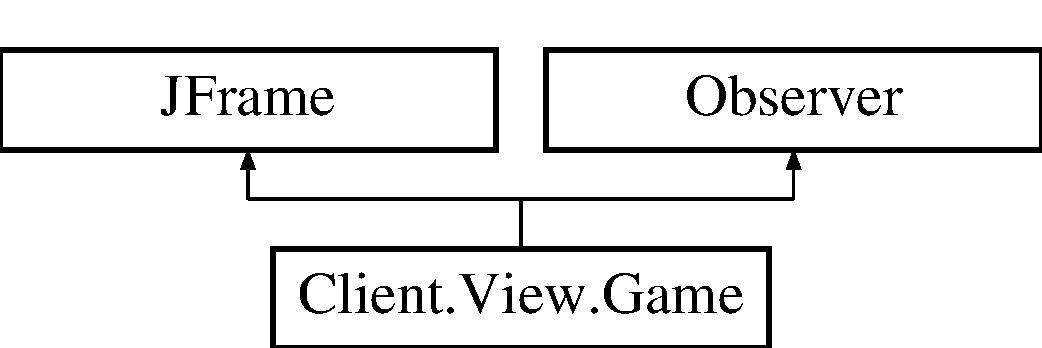
\includegraphics[height=2.000000cm]{a00038}
\end{center}
\end{figure}
\subsubsection*{Öffentliche Methoden}
\begin{DoxyCompactItemize}
\item 
\hyperlink{a00038_afe6d788e3d6d0c2b8f052d966bf6cea1}{Game} ()  throws I\-O\-Exception 
\item 
void \hyperlink{a00038_af04de16e7780bba7e3acab2554390b80}{update} (Observable o, Object arg)
\end{DoxyCompactItemize}


\subsubsection{Ausführliche Beschreibung}
Außerdem können über ein Dropdown-\/\-Menü Änderungen an Hintergrundbild und Kartenhintergründen vorgenommen werden. Schließen beendet das Spiel und der Spieler wird in die \hyperlink{a00053}{Lobby} zurückgeleitet.

\begin{DoxyAuthor}{Autor}
M4nkey 
\end{DoxyAuthor}


\subsubsection{Beschreibung der Konstruktoren und Destruktoren}
\hypertarget{a00038_afe6d788e3d6d0c2b8f052d966bf6cea1}{\index{Client\-::\-View\-::\-Game@{Client\-::\-View\-::\-Game}!Game@{Game}}
\index{Game@{Game}!Client::View::Game@{Client\-::\-View\-::\-Game}}
\paragraph[{Game}]{\setlength{\rightskip}{0pt plus 5cm}Client.\-View.\-Game.\-Game (
\begin{DoxyParamCaption}
{}
\end{DoxyParamCaption}
) throws I\-O\-Exception}}\label{a00038_afe6d788e3d6d0c2b8f052d966bf6cea1}


Erstellt das \hyperlink{a00038}{Game} Fenster. 


\begin{DoxyExceptions}{Ausnahmebehandlung}
{\em I\-O\-Exception} & \\
\hline
\end{DoxyExceptions}


\subsubsection{Dokumentation der Elementfunktionen}
\hypertarget{a00038_af04de16e7780bba7e3acab2554390b80}{\index{Client\-::\-View\-::\-Game@{Client\-::\-View\-::\-Game}!update@{update}}
\index{update@{update}!Client::View::Game@{Client\-::\-View\-::\-Game}}
\paragraph[{update}]{\setlength{\rightskip}{0pt plus 5cm}void Client.\-View.\-Game.\-update (
\begin{DoxyParamCaption}
\item[{Observable}]{o, }
\item[{Object}]{arg}
\end{DoxyParamCaption}
)}}\label{a00038_af04de16e7780bba7e3acab2554390b80}


Wird durch notify() im \hyperlink{a00013}{Client\-Model} aufgerufen. 

Je nach dem in arg übergebenen Befehl wird ein Update des Fensters ausgeführt oder eine Fehlermeldung angezeigt.


\begin{DoxyParams}{Parameter}
{\em o} & erwartet ein Objekt von der Klasse \hyperlink{a00013}{Client\-Model} \\
\hline
{\em arg} & erwartet\-: chat\-Message, played\-Cards\-Update, other\-Data\-Update \\
\hline
\end{DoxyParams}

\hypertarget{a00039}{\subsection{Com\-Server\-Acknowledgement Klassenreferenz}
\label{a00039}\index{Com\-Server\-Acknowledgement@{Com\-Server\-Acknowledgement}}
}


Abgeleitet von \hyperlink{a00037}{Com\-Object} und Serializable.

\subsubsection*{Öffentliche Methoden}
\begin{DoxyCompactItemize}
\item 
void \hyperlink{a00039_a758d7005755a181717f238f714d87dd2}{process} (\hyperlink{a00003}{Client\-Model} model)
\item 
void \hyperlink{a00039_ac67b5ce3ec03d48ef1e6caad6e49c902}{process} (\hyperlink{a00076}{Player} player, \hyperlink{a00077}{Server} server)
\end{DoxyCompactItemize}


\subsubsection{Ausführliche Beschreibung}
Diese Klasse ist ein spezielles Kommunikations-\/\-Objekt. Diese Nachricht wird vom Server als Bestaetigung gesendet. 

\subsubsection{Dokumentation der Elementfunktionen}
\hypertarget{a00039_a758d7005755a181717f238f714d87dd2}{\index{Com\-Objects\-::\-Com\-Server\-Acknowledgement@{Com\-Objects\-::\-Com\-Server\-Acknowledgement}!process@{process}}
\index{process@{process}!ComObjects::ComServerAcknowledgement@{Com\-Objects\-::\-Com\-Server\-Acknowledgement}}
\paragraph[{process}]{\setlength{\rightskip}{0pt plus 5cm}void process (
\begin{DoxyParamCaption}
\item[{{\bf Client\-Model}}]{model}
\end{DoxyParamCaption}
)}}\label{a00039_a758d7005755a181717f238f714d87dd2}


Diese Methode ist noetig, damit der Client\-Listener\-Thread entscheiden kann welche Message das Object enthaelt und wie diese verarbeitet werden soll. 


\begin{DoxyParams}{Parameter}
{\em model} & ist das Client\-Model, welches übergeben wird, damit die ueberladene Methode richtig gewaehlt wird. \\
\hline
\end{DoxyParams}


Implementiert \hyperlink{a00037_a758d7005755a181717f238f714d87dd2}{Com\-Object}.

\hypertarget{a00039_ac67b5ce3ec03d48ef1e6caad6e49c902}{\index{Com\-Objects\-::\-Com\-Server\-Acknowledgement@{Com\-Objects\-::\-Com\-Server\-Acknowledgement}!process@{process}}
\index{process@{process}!ComObjects::ComServerAcknowledgement@{Com\-Objects\-::\-Com\-Server\-Acknowledgement}}
\paragraph[{process}]{\setlength{\rightskip}{0pt plus 5cm}void process (
\begin{DoxyParamCaption}
\item[{{\bf Player}}]{player, }
\item[{{\bf Server}}]{server}
\end{DoxyParamCaption}
)}}\label{a00039_ac67b5ce3ec03d48ef1e6caad6e49c902}


Diese Methode ist noetig, damit der Thread Player entscheiden kann welche Message das Object enthaelt und wie diese verarbeitet werden soll. 


\begin{DoxyParams}{Parameter}
{\em player} & Der Client welcher den Aufruf startet. \\
\hline
{\em server} & Der Server an den sich das Com\-Objekt weitergibt. \\
\hline
\end{DoxyParams}


Implementiert \hyperlink{a00037_ac67b5ce3ec03d48ef1e6caad6e49c902}{Com\-Object}.


\hypertarget{a00040}{\subsection{Com\-Start\-Game Klassenreferenz}
\label{a00040}\index{Com\-Start\-Game@{Com\-Start\-Game}}
}


Abgeleitet von \hyperlink{a00037}{Com\-Object} und Serializable.

\subsubsection*{Öffentliche Methoden}
\begin{DoxyCompactItemize}
\item 
\hypertarget{a00040_a96b5e8f54fa85641a2f50624f4939202}{\hyperlink{a00040_a96b5e8f54fa85641a2f50624f4939202}{Com\-Start\-Game} ()}\label{a00040_a96b5e8f54fa85641a2f50624f4939202}

\item 
void \hyperlink{a00040_a758d7005755a181717f238f714d87dd2}{process} (\hyperlink{a00003}{Client\-Model} model)
\item 
void \hyperlink{a00040_ac67b5ce3ec03d48ef1e6caad6e49c902}{process} (\hyperlink{a00076}{Player} player, \hyperlink{a00077}{Server} server)
\end{DoxyCompactItemize}


\subsubsection{Ausführliche Beschreibung}
Diese Klasse ist ein spezielles Kommunikations-\/\-Objekt. Sie wird versendet, wenn ein Spiel gestartet werden soll. 

\subsubsection{Dokumentation der Elementfunktionen}
\hypertarget{a00040_a758d7005755a181717f238f714d87dd2}{\index{Com\-Objects\-::\-Com\-Start\-Game@{Com\-Objects\-::\-Com\-Start\-Game}!process@{process}}
\index{process@{process}!ComObjects::ComStartGame@{Com\-Objects\-::\-Com\-Start\-Game}}
\paragraph[{process}]{\setlength{\rightskip}{0pt plus 5cm}void process (
\begin{DoxyParamCaption}
\item[{{\bf Client\-Model}}]{model}
\end{DoxyParamCaption}
)}}\label{a00040_a758d7005755a181717f238f714d87dd2}


Diese Methode ist noetig, damit der Client\-Listener\-Thread entscheiden kann welche Message das Object enthaelt und wie diese verarbeitet werden soll. 


\begin{DoxyParams}{Parameter}
{\em model} & ist das Client\-Model, welches übergeben wird, damit die ueberladene Methode richtig gewaehlt wird. \\
\hline
\end{DoxyParams}


Implementiert \hyperlink{a00037_a758d7005755a181717f238f714d87dd2}{Com\-Object}.

\hypertarget{a00040_ac67b5ce3ec03d48ef1e6caad6e49c902}{\index{Com\-Objects\-::\-Com\-Start\-Game@{Com\-Objects\-::\-Com\-Start\-Game}!process@{process}}
\index{process@{process}!ComObjects::ComStartGame@{Com\-Objects\-::\-Com\-Start\-Game}}
\paragraph[{process}]{\setlength{\rightskip}{0pt plus 5cm}void process (
\begin{DoxyParamCaption}
\item[{{\bf Player}}]{player, }
\item[{{\bf Server}}]{server}
\end{DoxyParamCaption}
)}}\label{a00040_ac67b5ce3ec03d48ef1e6caad6e49c902}


Diese Methode ist noetig, damit der Thread Player entscheiden kann welche Message das Object enthaelt und wie diese verarbeitet werden soll. 


\begin{DoxyParams}{Parameter}
{\em player} & Der Client welcher den Aufruf startet. \\
\hline
{\em server} & Der Server an den sich das Com\-Objekt weitergibt. \\
\hline
\end{DoxyParams}


Implementiert \hyperlink{a00037_ac67b5ce3ec03d48ef1e6caad6e49c902}{Com\-Object}.


\hypertarget{a00041}{\subsection{Client.\-View.\-Game\-Panel Klassenreferenz}
\label{a00041}\index{Client.\-View.\-Game\-Panel@{Client.\-View.\-Game\-Panel}}
}
Klassendiagramm für Client.\-View.\-Game\-Panel\-:\begin{figure}[H]
\begin{center}
\leavevmode
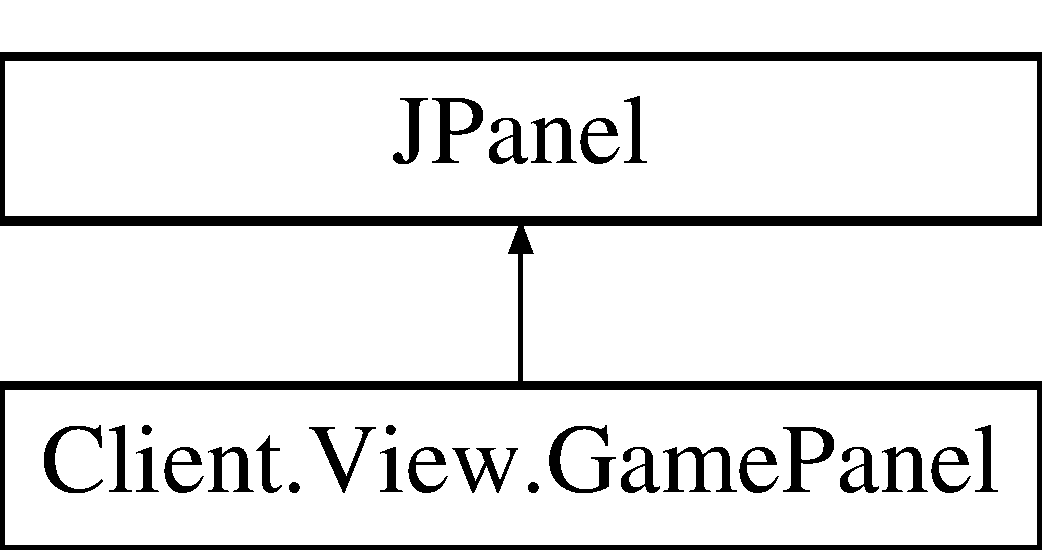
\includegraphics[height=2.000000cm]{a00041}
\end{center}
\end{figure}


\subsubsection{Ausführliche Beschreibung}
Es besteht aus veschiedenen Panelobjekten, welche je nach Regelwerk auf das Spielfeld gezeichnet werden. Dazu geh�ren die eigenen Karten, eventuell ausgew�hlte Karten, ein Textfeld z.\-B. zur Anzeige der Anzahl der restlichen Karten der Mitspieler und den Ablagestapel (/\-L194/). Nach jeder Runde wird der Punktestand aktualisiert.

\begin{DoxyAuthor}{Autor}
m4nkey 
\end{DoxyAuthor}

\hypertarget{a00042}{\subsection{Ruleset.\-Game\-Phase Enum-\/\-Referenz}
\label{a00042}\index{Ruleset.\-Game\-Phase@{Ruleset.\-Game\-Phase}}
}

\hypertarget{a00043}{\subsection{Server.\-Game\-Server Klassenreferenz}
\label{a00043}\index{Server.\-Game\-Server@{Server.\-Game\-Server}}
}
Klassendiagramm für Server.\-Game\-Server\-:\begin{figure}[H]
\begin{center}
\leavevmode
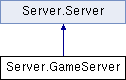
\includegraphics[height=2.000000cm]{a00043}
\end{center}
\end{figure}
\subsubsection*{Öffentliche Methoden}
\begin{DoxyCompactItemize}
\item 
\hyperlink{a00043_a6db144e60c51cb6ee80f448104127aed}{Game\-Server} (\hyperlink{a00054}{Lobby\-Server} server, \hyperlink{a00073}{Player} game\-Master, String Game\-Name, \hyperlink{a00076}{Ruleset\-Type} ruleset, String password, boolean has\-Password)
\item 
synchronized void \hyperlink{a00043_a942046c7512e4fead06f7df12faa119f}{add\-Player} (\hyperlink{a00073}{Player} player)
\item 
synchronized void \hyperlink{a00043_afc6cc835652484da1b7b1fda6071ea0b}{remove\-Player} (\hyperlink{a00073}{Player} player)
\item 
void \hyperlink{a00043_aae9201e5827933e23b078bc7eaf2aee3}{receive\-Message} (\hyperlink{a00073}{Player} player, Com\-Kick\-Player\-Request kick\-Player)
\item 
void \hyperlink{a00043_a7112c8a4b95e71c42a207b844f447305}{receive\-Message} (\hyperlink{a00073}{Player} player, Com\-Chat\-Message chat)
\item 
void \hyperlink{a00043_a9fd05e79a3ae006b056cb27199ee7aeb}{receive\-Message} (\hyperlink{a00073}{Player} player, Com\-Client\-Leave leave)
\item 
void \hyperlink{a00043_af3affa434fc5afd574d4fa74060ac9c7}{receive\-Message} (\hyperlink{a00073}{Player} player, Com\-Client\-Quit quit)
\item 
void \hyperlink{a00043_accca048ccec6323df6d3262f96d98723}{receive\-Message} (\hyperlink{a00073}{Player} player, Com\-Start\-Game start)
\item 
void \hyperlink{a00043_accad199750d7c6577b2d096483ce6e9d}{receive\-Message} (\hyperlink{a00073}{Player} player, Com\-Ruleset ruleset)
\item 
Com\-Init\-Game\-Lobby \hyperlink{a00043_a4e2b83f3466ec6c9cbe0a24a30587333}{init\-Lobby} ()
\end{DoxyCompactItemize}


\subsubsection{Ausführliche Beschreibung}
Sie verwaltet die Kommunikation zwischen den Clients w�hrend eines Spieles. Die Game\-Server-\/\-Klasse erbt Methoden zur Kommunikation vom \hyperlink{a00078}{Server}. Der \hyperlink{a00043}{Game\-Server} tauscht Nachrichten zwischen Ruleset und \hyperlink{a00073}{Player} aus, um so den Spielablauf zu koordinieren. \begin{DoxyAuthor}{Autor}
Viktoria 
\end{DoxyAuthor}


\subsubsection{Beschreibung der Konstruktoren und Destruktoren}
\hypertarget{a00043_a6db144e60c51cb6ee80f448104127aed}{\index{Server\-::\-Game\-Server@{Server\-::\-Game\-Server}!Game\-Server@{Game\-Server}}
\index{Game\-Server@{Game\-Server}!Server::GameServer@{Server\-::\-Game\-Server}}
\paragraph[{Game\-Server}]{\setlength{\rightskip}{0pt plus 5cm}Server.\-Game\-Server.\-Game\-Server (
\begin{DoxyParamCaption}
\item[{{\bf Lobby\-Server}}]{server, }
\item[{{\bf Player}}]{game\-Master, }
\item[{String}]{Game\-Name, }
\item[{{\bf Ruleset\-Type}}]{ruleset, }
\item[{String}]{password, }
\item[{boolean}]{has\-Password}
\end{DoxyParamCaption}
)}}\label{a00043_a6db144e60c51cb6ee80f448104127aed}


Konstruktor des Game\-Servers. 

Setzt die Attribute lobby\-Server, name, password, has\-Pasword und ruleset\-Type auf die �bergebenen Werte. Setzt den game\-Master\-Name auf den Namen des game\-Master und f�gt den game\-Master dem Set an Spielern hinzu. Bestimmt mithilfe des Enums Ruleset\-Type das Ruleset und erstellt es. Setzt current\-Players auf eins und max\-Players je nach Ruleset. 
\begin{DoxyParams}{Parameter}
{\em server} & ist der \hyperlink{a00054}{Lobby\-Server} der den \hyperlink{a00043}{Game\-Server} erstellt hat. \\
\hline
{\em game\-Master} & ist der Name des Spielleiters \\
\hline
{\em Game\-Name} & ist der Name des Spiels \\
\hline
{\em ruleset} & gibt an, welches Ruleset verwendet wird \\
\hline
{\em password} & speichert das Passwort des Spiels \\
\hline
{\em has\-Password} & gibt an,ob das Spiel ein Passwort hat \\
\hline
\end{DoxyParams}


\subsubsection{Dokumentation der Elementfunktionen}
\hypertarget{a00043_a942046c7512e4fead06f7df12faa119f}{\index{Server\-::\-Game\-Server@{Server\-::\-Game\-Server}!add\-Player@{add\-Player}}
\index{add\-Player@{add\-Player}!Server::GameServer@{Server\-::\-Game\-Server}}
\paragraph[{add\-Player}]{\setlength{\rightskip}{0pt plus 5cm}synchronized void Server.\-Game\-Server.\-add\-Player (
\begin{DoxyParamCaption}
\item[{{\bf Player}}]{player}
\end{DoxyParamCaption}
)}}\label{a00043_a942046c7512e4fead06f7df12faa119f}


Diese Methode wird vom abstrakten \hyperlink{a00078}{Server} vererbt. 

Zus�tzlich wird die Zahl der current\-Players um eins Erh�ht. 
\begin{DoxyParams}{Parameter}
{\em player} & ist der \hyperlink{a00073}{Player}, der hinzugefo�gt wird \\
\hline
\end{DoxyParams}
\hypertarget{a00043_a4e2b83f3466ec6c9cbe0a24a30587333}{\index{Server\-::\-Game\-Server@{Server\-::\-Game\-Server}!init\-Lobby@{init\-Lobby}}
\index{init\-Lobby@{init\-Lobby}!Server::GameServer@{Server\-::\-Game\-Server}}
\paragraph[{init\-Lobby}]{\setlength{\rightskip}{0pt plus 5cm}Com\-Init\-Game\-Lobby Server.\-Game\-Server.\-init\-Lobby (
\begin{DoxyParamCaption}
{}
\end{DoxyParamCaption}
)}}\label{a00043_a4e2b83f3466ec6c9cbe0a24a30587333}


Baut ein neues Com\-Init\-Game\-Lobby Objekt und gibt es zur�ck. 

\begin{DoxyReturn}{Rückgabe}
Gibt das Com\-Init\-Game\-Lobby Objekt zur�ck 
\end{DoxyReturn}
\hypertarget{a00043_aae9201e5827933e23b078bc7eaf2aee3}{\index{Server\-::\-Game\-Server@{Server\-::\-Game\-Server}!receive\-Message@{receive\-Message}}
\index{receive\-Message@{receive\-Message}!Server::GameServer@{Server\-::\-Game\-Server}}
\paragraph[{receive\-Message}]{\setlength{\rightskip}{0pt plus 5cm}void Server.\-Game\-Server.\-receive\-Message (
\begin{DoxyParamCaption}
\item[{{\bf Player}}]{player, }
\item[{Com\-Kick\-Player\-Request}]{kick\-Player}
\end{DoxyParamCaption}
)}}\label{a00043_aae9201e5827933e23b078bc7eaf2aee3}


Diese Methode ist dafur zust�ndig zu ermitteln, was passiert wenn ein Spieler aus der Game\-Lobby geworfen wird. 

Der \hyperlink{a00073}{Player} wird durch Aufruf von change\-Server an die Lobby zur�ckgegeben. An diesen Spieler wird ein Com\-Warning und ein Com\-Init\-Lobby geschickt. Danach wird ein Com\-Update\-Playerlist Objekt mit broadcast an alle Client im Spiel verschickt. 
\begin{DoxyParams}{Parameter}
{\em player} & ist der Threat der die Nachricht erhalten hat \\
\hline
{\em kicked} & ist das Com\-Object, das verarbeitet wird \\
\hline
\end{DoxyParams}
\hypertarget{a00043_a7112c8a4b95e71c42a207b844f447305}{\index{Server\-::\-Game\-Server@{Server\-::\-Game\-Server}!receive\-Message@{receive\-Message}}
\index{receive\-Message@{receive\-Message}!Server::GameServer@{Server\-::\-Game\-Server}}
\paragraph[{receive\-Message}]{\setlength{\rightskip}{0pt plus 5cm}void Server.\-Game\-Server.\-receive\-Message (
\begin{DoxyParamCaption}
\item[{{\bf Player}}]{player, }
\item[{Com\-Chat\-Message}]{chat}
\end{DoxyParamCaption}
)}}\label{a00043_a7112c8a4b95e71c42a207b844f447305}


Diese Methode ist dafur zust�ndig eine Chatnachricht an alle Clients im Spiel zu verschicken. 

Daf�r wird die Com\-Chat\-Message mit broadcast an alle Spieler im player\-Set verteilt. 
\begin{DoxyParams}{Parameter}
{\em player} & ist der Threat der die Nachricht erhalten hat \\
\hline
{\em chat} & ist das Com\-Object, das die Chatnachricht enth�lt \\
\hline
\end{DoxyParams}
\hypertarget{a00043_a9fd05e79a3ae006b056cb27199ee7aeb}{\index{Server\-::\-Game\-Server@{Server\-::\-Game\-Server}!receive\-Message@{receive\-Message}}
\index{receive\-Message@{receive\-Message}!Server::GameServer@{Server\-::\-Game\-Server}}
\paragraph[{receive\-Message}]{\setlength{\rightskip}{0pt plus 5cm}void Server.\-Game\-Server.\-receive\-Message (
\begin{DoxyParamCaption}
\item[{{\bf Player}}]{player, }
\item[{Com\-Client\-Leave}]{leave}
\end{DoxyParamCaption}
)}}\label{a00043_a9fd05e79a3ae006b056cb27199ee7aeb}


Diese Methode gibt einen \hyperlink{a00073}{Player}, der die Game\-Lobby verlassen will, durch Aufruf von change\-Server an die Server\-Lobby zur�ck und schickt ihm ein Com\-Init\-Lobby. 

Danach wird ein Com\-Update\-Playerlist Objekt mit broadcast an alle Clients im Spiel verschickt. 
\begin{DoxyParams}{Parameter}
{\em player} & ist der Threat der die Nachricht erhalten hat \\
\hline
{\em leave} & ist das Com\-Object, welches angibt, dass der Spieler in die Lobby zur�ckkehrt \\
\hline
\end{DoxyParams}
\hypertarget{a00043_af3affa434fc5afd574d4fa74060ac9c7}{\index{Server\-::\-Game\-Server@{Server\-::\-Game\-Server}!receive\-Message@{receive\-Message}}
\index{receive\-Message@{receive\-Message}!Server::GameServer@{Server\-::\-Game\-Server}}
\paragraph[{receive\-Message}]{\setlength{\rightskip}{0pt plus 5cm}void Server.\-Game\-Server.\-receive\-Message (
\begin{DoxyParamCaption}
\item[{{\bf Player}}]{player, }
\item[{Com\-Client\-Quit}]{quit}
\end{DoxyParamCaption}
)}}\label{a00043_af3affa434fc5afd574d4fa74060ac9c7}


Diese Methode behandelt den Fall, dass ein Spieler das laufende Spiel verl�sst. 

Sie gibt einen \hyperlink{a00073}{Player}, der das Spiel verlassen will, Aufruf von change\-Server an die Server\-Lobby zur�ck und schickt ihm ein Com\-Init\-Lobby. Alle Spieler, die sich im Spiel befinden bekommen ein Com\-Warning und ein Com\-Init\-Lobby und werden durch Aufruf von change\-Server an die Lobby zur�ckgegeben. Das Spiel wird aufgel�st. 
\begin{DoxyParams}{Parameter}
{\em player} & ist der Threat der die Nachricht erhalten hat \\
\hline
{\em quit} & ist das Com\-Object, welches angibt, dass der Spieler das Spiel verl�sst \\
\hline
\end{DoxyParams}
\hypertarget{a00043_accca048ccec6323df6d3262f96d98723}{\index{Server\-::\-Game\-Server@{Server\-::\-Game\-Server}!receive\-Message@{receive\-Message}}
\index{receive\-Message@{receive\-Message}!Server::GameServer@{Server\-::\-Game\-Server}}
\paragraph[{receive\-Message}]{\setlength{\rightskip}{0pt plus 5cm}void Server.\-Game\-Server.\-receive\-Message (
\begin{DoxyParamCaption}
\item[{{\bf Player}}]{player, }
\item[{Com\-Start\-Game}]{start}
\end{DoxyParamCaption}
)}}\label{a00043_accca048ccec6323df6d3262f96d98723}


Diese Methode sagt dem Ruleset, dass ein neues Spiel gestartet werden soll. 


\begin{DoxyParams}{Parameter}
{\em player} & ist der Threat der die Nachricht erhalten hat \\
\hline
{\em start} & ist das Com\-Object, dass angibt, dass das Spiel gestartet werden soll \\
\hline
\end{DoxyParams}
\hypertarget{a00043_accad199750d7c6577b2d096483ce6e9d}{\index{Server\-::\-Game\-Server@{Server\-::\-Game\-Server}!receive\-Message@{receive\-Message}}
\index{receive\-Message@{receive\-Message}!Server::GameServer@{Server\-::\-Game\-Server}}
\paragraph[{receive\-Message}]{\setlength{\rightskip}{0pt plus 5cm}void Server.\-Game\-Server.\-receive\-Message (
\begin{DoxyParamCaption}
\item[{{\bf Player}}]{player, }
\item[{Com\-Ruleset}]{ruleset}
\end{DoxyParamCaption}
)}}\label{a00043_accad199750d7c6577b2d096483ce6e9d}


Diese Methode gibt das erhaltene Com\-Ruleset durch einen Aufruf von resolve\-Message an das Ruleset weiter. 


\begin{DoxyParams}{Parameter}
{\em player} & ist der Threat der die Nachricht erhalten hat \\
\hline
{\em ruleset} & ist das Com\-Object, das zeigt, dass das Object vom Ruleset bearbeitet werden muss \\
\hline
\end{DoxyParams}
\hypertarget{a00043_afc6cc835652484da1b7b1fda6071ea0b}{\index{Server\-::\-Game\-Server@{Server\-::\-Game\-Server}!remove\-Player@{remove\-Player}}
\index{remove\-Player@{remove\-Player}!Server::GameServer@{Server\-::\-Game\-Server}}
\paragraph[{remove\-Player}]{\setlength{\rightskip}{0pt plus 5cm}synchronized void Server.\-Game\-Server.\-remove\-Player (
\begin{DoxyParamCaption}
\item[{{\bf Player}}]{player}
\end{DoxyParamCaption}
)}}\label{a00043_afc6cc835652484da1b7b1fda6071ea0b}


Diese Methode wird vom abstrakten \hyperlink{a00078}{Server} vererbt. 

Zus�tzlich wird die Zahl der current\-Players um eins Verringert. 
\begin{DoxyParams}{Parameter}
{\em player} & ist der \hyperlink{a00073}{Player}, der entfernt wird \\
\hline
\end{DoxyParams}

\hypertarget{a00044}{\subsection{Server.\-Game\-Server\-Representation Klassenreferenz}
\label{a00044}\index{Server.\-Game\-Server\-Representation@{Server.\-Game\-Server\-Representation}}
}
\subsubsection*{Öffentliche Methoden}
\begin{DoxyCompactItemize}
\item 
\hyperlink{a00044_afabe1ef940660d5ccde15467933d0ad0}{Game\-Server\-Representation} (String game\-Master, String game\-Name, int max, int current, \hyperlink{a00076}{Ruleset\-Type} type, boolean password)
\end{DoxyCompactItemize}


\subsubsection{Ausführliche Beschreibung}
Sie wird dem Com\-Objekt Com\-Lobby\-Update\-Game\-List angehängt, um die Spielliste in der Game\-Lobby aktualisieren zu können \begin{DoxyAuthor}{Autor}
Viktoria 
\end{DoxyAuthor}


\subsubsection{Beschreibung der Konstruktoren und Destruktoren}
\hypertarget{a00044_afabe1ef940660d5ccde15467933d0ad0}{\index{Server\-::\-Game\-Server\-Representation@{Server\-::\-Game\-Server\-Representation}!Game\-Server\-Representation@{Game\-Server\-Representation}}
\index{Game\-Server\-Representation@{Game\-Server\-Representation}!Server::GameServerRepresentation@{Server\-::\-Game\-Server\-Representation}}
\paragraph[{Game\-Server\-Representation}]{\setlength{\rightskip}{0pt plus 5cm}Server.\-Game\-Server\-Representation.\-Game\-Server\-Representation (
\begin{DoxyParamCaption}
\item[{String}]{game\-Master, }
\item[{String}]{game\-Name, }
\item[{int}]{max, }
\item[{int}]{current, }
\item[{{\bf Ruleset\-Type}}]{type, }
\item[{boolean}]{password}
\end{DoxyParamCaption}
)}}\label{a00044_afabe1ef940660d5ccde15467933d0ad0}


Der Konstruktor der Klasse \hyperlink{a00044}{Game\-Server\-Representation} initialisiert die Attribute mit den vom \hyperlink{a00043}{Game\-Server} übergebenen Werten. 


\begin{DoxyParams}{Parameter}
{\em game\-Master} & der Name des Spielleiters \\
\hline
{\em game\-Name} & der Name des Spiels \\
\hline
{\em max} & Maximal mögliche Anzahl teilnehmender Spieler \\
\hline
{\em current} & Anzahl momentaner Spieler \\
\hline
{\em type} & Welches Ruleset verwendet wird \\
\hline
{\em password} & ob das Spiel ein Passwort hat \\
\hline
\end{DoxyParams}

\hypertarget{a00045}{\subsection{Ruleset.\-Game\-State Klassenreferenz}
\label{a00045}\index{Ruleset.\-Game\-State@{Ruleset.\-Game\-State}}
}
\subsubsection*{Öffentliche Methoden}
\begin{DoxyCompactItemize}
\item 
void \hyperlink{a00045_adcdd80db7006a129d2681ef2156d8030}{set\-Current\-Player} (\hyperlink{a00074}{Player\-State} player)
\item 
\hyperlink{a00074}{Player\-State} \hyperlink{a00045_a940b04c3b7b3e4b2a407b77fa40cce33}{get\-Current\-Player} ()
\item 
Array\-List$<$ \hyperlink{a00002}{Card} $>$ \hyperlink{a00045_acbb1847c191f8642f77c72b971663602}{get\-Cards\-Left\-In\-Deck} ()
\item 
Map$<$ String, \hyperlink{a00002}{Card} $>$ \hyperlink{a00045_a1c3dd6d0e4fd89dd49eb5073c1e06234}{get\-Played\-Cards} ()
\item 
\hyperlink{a00074}{Player\-State} \hyperlink{a00045_aa087b905d7f5b7ac4f7f3356b7d0f06d}{get\-Player} (String name)
\item 
void \hyperlink{a00045_a6cbf9650695639cdbccfc520cc9b112f}{set\-Trump\-Card} (\hyperlink{a00002}{Card} trump\-Card)
\item 
\hyperlink{a00002}{Card} \hyperlink{a00045_a263d6b7805c19249a3a1243379480e87}{get\-Trump\-Card} ()
\item 
int \hyperlink{a00045_afef5de42e97641f5f4f46c2995697502}{get\-Number\-Of\-Played\-Cards} ()
\item 
boolean \hyperlink{a00045_a53e85a9b7f4fe195604de0f1e8a59550}{play\-Card} (\hyperlink{a00002}{Card} card)
\end{DoxyCompactItemize}


\subsubsection{Ausführliche Beschreibung}
Es enthält die einzelnen Player\-States, sowie Informationen zum Ablage-\/, Aufnahmestapel, Rundenanzahl, den momentan aktiven Spieler sowie \hyperlink{a00042}{Game\-Phase}. 

\subsubsection{Dokumentation der Elementfunktionen}
\hypertarget{a00045_acbb1847c191f8642f77c72b971663602}{\index{Ruleset\-::\-Game\-State@{Ruleset\-::\-Game\-State}!get\-Cards\-Left\-In\-Deck@{get\-Cards\-Left\-In\-Deck}}
\index{get\-Cards\-Left\-In\-Deck@{get\-Cards\-Left\-In\-Deck}!Ruleset::GameState@{Ruleset\-::\-Game\-State}}
\paragraph[{get\-Cards\-Left\-In\-Deck}]{\setlength{\rightskip}{0pt plus 5cm}Array\-List$<${\bf Card}$>$ Ruleset.\-Game\-State.\-get\-Cards\-Left\-In\-Deck (
\begin{DoxyParamCaption}
{}
\end{DoxyParamCaption}
)}}\label{a00045_acbb1847c191f8642f77c72b971663602}


Holt die Karten die noch im Aufnahmestapel sind. 

\begin{DoxyReturn}{Rückgabe}
cards\-Left\-In\-Deck Holt die Karten die noch im Aufnahmestapel sind 
\end{DoxyReturn}
\hypertarget{a00045_a940b04c3b7b3e4b2a407b77fa40cce33}{\index{Ruleset\-::\-Game\-State@{Ruleset\-::\-Game\-State}!get\-Current\-Player@{get\-Current\-Player}}
\index{get\-Current\-Player@{get\-Current\-Player}!Ruleset::GameState@{Ruleset\-::\-Game\-State}}
\paragraph[{get\-Current\-Player}]{\setlength{\rightskip}{0pt plus 5cm}{\bf Player\-State} Ruleset.\-Game\-State.\-get\-Current\-Player (
\begin{DoxyParamCaption}
{}
\end{DoxyParamCaption}
)}}\label{a00045_a940b04c3b7b3e4b2a407b77fa40cce33}


Holt den Spieler der momentan am Zug ist. 

\begin{DoxyReturn}{Rückgabe}
current\-Player Der Spielzustand des Spielers der grad am Zug ist 
\end{DoxyReturn}
\hypertarget{a00045_afef5de42e97641f5f4f46c2995697502}{\index{Ruleset\-::\-Game\-State@{Ruleset\-::\-Game\-State}!get\-Number\-Of\-Played\-Cards@{get\-Number\-Of\-Played\-Cards}}
\index{get\-Number\-Of\-Played\-Cards@{get\-Number\-Of\-Played\-Cards}!Ruleset::GameState@{Ruleset\-::\-Game\-State}}
\paragraph[{get\-Number\-Of\-Played\-Cards}]{\setlength{\rightskip}{0pt plus 5cm}int Ruleset.\-Game\-State.\-get\-Number\-Of\-Played\-Cards (
\begin{DoxyParamCaption}
{}
\end{DoxyParamCaption}
)}}\label{a00045_afef5de42e97641f5f4f46c2995697502}


Holt die Anzahl der gespielten Karten. 

\begin{DoxyReturn}{Rückgabe}
Die Anzahl der gespielten Karten 
\end{DoxyReturn}
\hypertarget{a00045_a1c3dd6d0e4fd89dd49eb5073c1e06234}{\index{Ruleset\-::\-Game\-State@{Ruleset\-::\-Game\-State}!get\-Played\-Cards@{get\-Played\-Cards}}
\index{get\-Played\-Cards@{get\-Played\-Cards}!Ruleset::GameState@{Ruleset\-::\-Game\-State}}
\paragraph[{get\-Played\-Cards}]{\setlength{\rightskip}{0pt plus 5cm}Map$<$String,{\bf Card}$>$ Ruleset.\-Game\-State.\-get\-Played\-Cards (
\begin{DoxyParamCaption}
{}
\end{DoxyParamCaption}
)}}\label{a00045_a1c3dd6d0e4fd89dd49eb5073c1e06234}


Holt die gespielten Karten im Ablagestapel. 

\begin{DoxyReturn}{Rückgabe}


discard\-Pile Die gespielten Karten 
\end{DoxyReturn}
\hypertarget{a00045_aa087b905d7f5b7ac4f7f3356b7d0f06d}{\index{Ruleset\-::\-Game\-State@{Ruleset\-::\-Game\-State}!get\-Player@{get\-Player}}
\index{get\-Player@{get\-Player}!Ruleset::GameState@{Ruleset\-::\-Game\-State}}
\paragraph[{get\-Player}]{\setlength{\rightskip}{0pt plus 5cm}{\bf Player\-State} Ruleset.\-Game\-State.\-get\-Player (
\begin{DoxyParamCaption}
\item[{String}]{name}
\end{DoxyParamCaption}
)}}\label{a00045_aa087b905d7f5b7ac4f7f3356b7d0f06d}


Holt einen bestimmten Spieler. 


\begin{DoxyParams}{Parameter}
{\em name} & Der Name des Spielers \\
\hline
\end{DoxyParams}
\begin{DoxyReturn}{Rückgabe}
player Der Spielzustand des Spielers 
\end{DoxyReturn}
\hypertarget{a00045_a263d6b7805c19249a3a1243379480e87}{\index{Ruleset\-::\-Game\-State@{Ruleset\-::\-Game\-State}!get\-Trump\-Card@{get\-Trump\-Card}}
\index{get\-Trump\-Card@{get\-Trump\-Card}!Ruleset::GameState@{Ruleset\-::\-Game\-State}}
\paragraph[{get\-Trump\-Card}]{\setlength{\rightskip}{0pt plus 5cm}{\bf Card} Ruleset.\-Game\-State.\-get\-Trump\-Card (
\begin{DoxyParamCaption}
{}
\end{DoxyParamCaption}
)}}\label{a00045_a263d6b7805c19249a3a1243379480e87}


Holt die momentane Trumpfkarte im Spiel. 

\begin{DoxyReturn}{Rückgabe}
trump\-Card Die momentane Trumpfkarte 
\end{DoxyReturn}
\hypertarget{a00045_a53e85a9b7f4fe195604de0f1e8a59550}{\index{Ruleset\-::\-Game\-State@{Ruleset\-::\-Game\-State}!play\-Card@{play\-Card}}
\index{play\-Card@{play\-Card}!Ruleset::GameState@{Ruleset\-::\-Game\-State}}
\paragraph[{play\-Card}]{\setlength{\rightskip}{0pt plus 5cm}boolean Ruleset.\-Game\-State.\-play\-Card (
\begin{DoxyParamCaption}
\item[{{\bf Card}}]{card}
\end{DoxyParamCaption}
)}}\label{a00045_a53e85a9b7f4fe195604de0f1e8a59550}


Entfernt eine Karte aus der Hand des current\-Player und legt sie auf dem Ablagestapel. 


\begin{DoxyParams}{Parameter}
{\em card} & Die gespielte Karte \\
\hline
\end{DoxyParams}
\begin{DoxyReturn}{Rückgabe}
is\-In\-Hand Gibt true zurück wenn die gespielte Karte auf der Hand vom Spieler liegt und false sonst 
\end{DoxyReturn}
\hypertarget{a00045_adcdd80db7006a129d2681ef2156d8030}{\index{Ruleset\-::\-Game\-State@{Ruleset\-::\-Game\-State}!set\-Current\-Player@{set\-Current\-Player}}
\index{set\-Current\-Player@{set\-Current\-Player}!Ruleset::GameState@{Ruleset\-::\-Game\-State}}
\paragraph[{set\-Current\-Player}]{\setlength{\rightskip}{0pt plus 5cm}void Ruleset.\-Game\-State.\-set\-Current\-Player (
\begin{DoxyParamCaption}
\item[{{\bf Player\-State}}]{player}
\end{DoxyParamCaption}
)}}\label{a00045_adcdd80db7006a129d2681ef2156d8030}


Setzt einen neuen Spieler als current\-Player. 


\begin{DoxyParams}{Parameter}
{\em player} & Der neue current\-Player \\
\hline
\end{DoxyParams}
\hypertarget{a00045_a6cbf9650695639cdbccfc520cc9b112f}{\index{Ruleset\-::\-Game\-State@{Ruleset\-::\-Game\-State}!set\-Trump\-Card@{set\-Trump\-Card}}
\index{set\-Trump\-Card@{set\-Trump\-Card}!Ruleset::GameState@{Ruleset\-::\-Game\-State}}
\paragraph[{set\-Trump\-Card}]{\setlength{\rightskip}{0pt plus 5cm}void Ruleset.\-Game\-State.\-set\-Trump\-Card (
\begin{DoxyParamCaption}
\item[{{\bf Card}}]{trump\-Card}
\end{DoxyParamCaption}
)}}\label{a00045_a6cbf9650695639cdbccfc520cc9b112f}


Setzt die Trumpfkarte. 


\begin{DoxyParams}{Parameter}
{\em trump\-Card} & Die Trumpfkarte \\
\hline
\end{DoxyParams}

\hypertarget{a00046}{\subsection{Msg\-Multi\-Cards Klassenreferenz}
\label{a00046}\index{Msg\-Multi\-Cards@{Msg\-Multi\-Cards}}
}


Abgeleitet von \hyperlink{a00053}{Ruleset\-Message} und Serializable.

\subsubsection*{Öffentliche Methoden}
\begin{DoxyCompactItemize}
\item 
\hyperlink{a00046_a4bb40ccd570d979fcef33ffafb5c23a9}{Msg\-Multi\-Cards} (Set card\-List)
\item 
Set$<$ \hyperlink{a00054}{Card} $>$ \hyperlink{a00046_a84a6c04ecb3d13ea4a456862ac72cdf6}{get\-Card\-List} ()
\item 
void \hyperlink{a00046_ab45288da8f64e79408f1effd5579b5c2}{visit} (\hyperlink{a00068}{Server\-Ruleset} server\-Ruleset, String name)
\item 
void \hyperlink{a00046_acb5be722a2d1c9110d39f31c6e18f6e7}{visit} (\hyperlink{a00056}{Client\-Ruleset} client\-Ruleset)
\end{DoxyCompactItemize}
\subsubsection*{Private Attribute}
\begin{DoxyCompactItemize}
\item 
\hypertarget{a00046_a2994bb7f93a3ba7462f42533b4625649}{Set$<$ \hyperlink{a00054}{Card} $>$ {\bfseries card\-List}}\label{a00046_a2994bb7f93a3ba7462f42533b4625649}

\end{DoxyCompactItemize}


\subsubsection{Ausführliche Beschreibung}
Diese Klasse ist eine Verfeinerung der Ruleset\-Message-\/\-Klasse. Sie liefert mehrere Karten zum Tausch fuer das Regelwerk Hearts. 

\subsubsection{Beschreibung der Konstruktoren und Destruktoren}
\hypertarget{a00046_a4bb40ccd570d979fcef33ffafb5c23a9}{\index{Com\-Objects\-::\-Msg\-Multi\-Cards@{Com\-Objects\-::\-Msg\-Multi\-Cards}!Msg\-Multi\-Cards@{Msg\-Multi\-Cards}}
\index{Msg\-Multi\-Cards@{Msg\-Multi\-Cards}!ComObjects::MsgMultiCards@{Com\-Objects\-::\-Msg\-Multi\-Cards}}
\paragraph[{Msg\-Multi\-Cards}]{\setlength{\rightskip}{0pt plus 5cm}{\bf Msg\-Multi\-Cards} (
\begin{DoxyParamCaption}
\item[{Set}]{card\-List}
\end{DoxyParamCaption}
)}}\label{a00046_a4bb40ccd570d979fcef33ffafb5c23a9}


Dies ist der Kontruktor fuer eine neue Msg\-Multi\-Cards-\/\-Nachricht. 


\begin{DoxyParams}{Parameter}
{\em card\-List} & ist die Liste der ausgewaehlten Karten. \\
\hline
\end{DoxyParams}


\subsubsection{Dokumentation der Elementfunktionen}
\hypertarget{a00046_a84a6c04ecb3d13ea4a456862ac72cdf6}{\index{Com\-Objects\-::\-Msg\-Multi\-Cards@{Com\-Objects\-::\-Msg\-Multi\-Cards}!get\-Card\-List@{get\-Card\-List}}
\index{get\-Card\-List@{get\-Card\-List}!ComObjects::MsgMultiCards@{Com\-Objects\-::\-Msg\-Multi\-Cards}}
\paragraph[{get\-Card\-List}]{\setlength{\rightskip}{0pt plus 5cm}Set$<${\bf Card}$>$ get\-Card\-List (
\begin{DoxyParamCaption}
{}
\end{DoxyParamCaption}
)}}\label{a00046_a84a6c04ecb3d13ea4a456862ac72cdf6}


Gibt die Liste der gewaehlten Karten zurück. 

\begin{DoxyReturn}{Rückgabe}
die Liste der Karten. 
\end{DoxyReturn}
\hypertarget{a00046_ab45288da8f64e79408f1effd5579b5c2}{\index{Com\-Objects\-::\-Msg\-Multi\-Cards@{Com\-Objects\-::\-Msg\-Multi\-Cards}!visit@{visit}}
\index{visit@{visit}!ComObjects::MsgMultiCards@{Com\-Objects\-::\-Msg\-Multi\-Cards}}
\paragraph[{visit}]{\setlength{\rightskip}{0pt plus 5cm}void visit (
\begin{DoxyParamCaption}
\item[{{\bf Server\-Ruleset}}]{server\-Ruleset, }
\item[{String}]{name}
\end{DoxyParamCaption}
)}}\label{a00046_ab45288da8f64e79408f1effd5579b5c2}


Diese Methode ist noetig, damit das Server\-Ruleset entscheiden kann welche Message es enthaelt und wie diese verarbeitet werden soll. 


\begin{DoxyParams}{Parameter}
{\em server\-Ruleset} & ist das Ruleset, welches übergeben wird, damit die ueberladene Methode richtig gewaehlt wird. \\
\hline
{\em name} & ist der Name des Spielers. \\
\hline
\end{DoxyParams}


Implementiert \hyperlink{a00053_ab45288da8f64e79408f1effd5579b5c2}{Ruleset\-Message}.

\hypertarget{a00046_acb5be722a2d1c9110d39f31c6e18f6e7}{\index{Com\-Objects\-::\-Msg\-Multi\-Cards@{Com\-Objects\-::\-Msg\-Multi\-Cards}!visit@{visit}}
\index{visit@{visit}!ComObjects::MsgMultiCards@{Com\-Objects\-::\-Msg\-Multi\-Cards}}
\paragraph[{visit}]{\setlength{\rightskip}{0pt plus 5cm}void visit (
\begin{DoxyParamCaption}
\item[{{\bf Client\-Ruleset}}]{client\-Ruleset}
\end{DoxyParamCaption}
)}}\label{a00046_acb5be722a2d1c9110d39f31c6e18f6e7}


Diese Methode ist noetig, damit das Client\-Ruleset entscheiden kann welche Message es enthaelt und wie diese verarbeitet werden soll. 


\begin{DoxyParams}{Parameter}
{\em client\-Ruleset} & ist das Ruleset, welches uebergeben wird, damit die ueberladene Methode richtig gewaehlt wird. \\
\hline
\end{DoxyParams}


Implementiert \hyperlink{a00053_acb5be722a2d1c9110d39f31c6e18f6e7}{Ruleset\-Message}.


\hypertarget{a00047}{\subsection{Msg\-Multi\-Cards\-Request Klassenreferenz}
\label{a00047}\index{Msg\-Multi\-Cards\-Request@{Msg\-Multi\-Cards\-Request}}
}


Abgeleitet von \hyperlink{a00053}{Ruleset\-Message} und Serializable.

\subsubsection*{Öffentliche Methoden}
\begin{DoxyCompactItemize}
\item 
\hyperlink{a00047_a8bddd71e746b26a73e6f873006972fcb}{Msg\-Multi\-Cards\-Request} (int \hyperlink{a00047_ad43c3812e6d13e0518d9f8b8f463ffcf}{count})
\item 
int \hyperlink{a00047_ae452b1c7e00c383f2916c4a530fab737}{get\-Count} ()
\item 
void \hyperlink{a00047_ab45288da8f64e79408f1effd5579b5c2}{visit} (\hyperlink{a00068}{Server\-Ruleset} server\-Ruleset, String name)
\item 
void \hyperlink{a00047_acb5be722a2d1c9110d39f31c6e18f6e7}{visit} (\hyperlink{a00056}{Client\-Ruleset} client\-Ruleset)
\end{DoxyCompactItemize}
\subsubsection*{Private Attribute}
\begin{DoxyCompactItemize}
\item 
\hypertarget{a00047_ad43c3812e6d13e0518d9f8b8f463ffcf}{int \hyperlink{a00047_ad43c3812e6d13e0518d9f8b8f463ffcf}{count}}\label{a00047_ad43c3812e6d13e0518d9f8b8f463ffcf}

\end{DoxyCompactItemize}


\subsubsection{Ausführliche Beschreibung}
Diese Klasse ist eine Verfeinerung der Ruleset\-Message-\/\-Klasse. Diese Nachricht wird gesendet, wenn die Auswahl mehrerer Karten vom Spieler gefordert werden soll. 

\subsubsection{Beschreibung der Konstruktoren und Destruktoren}
\hypertarget{a00047_a8bddd71e746b26a73e6f873006972fcb}{\index{Com\-Objects\-::\-Msg\-Multi\-Cards\-Request@{Com\-Objects\-::\-Msg\-Multi\-Cards\-Request}!Msg\-Multi\-Cards\-Request@{Msg\-Multi\-Cards\-Request}}
\index{Msg\-Multi\-Cards\-Request@{Msg\-Multi\-Cards\-Request}!ComObjects::MsgMultiCardsRequest@{Com\-Objects\-::\-Msg\-Multi\-Cards\-Request}}
\paragraph[{Msg\-Multi\-Cards\-Request}]{\setlength{\rightskip}{0pt plus 5cm}{\bf Msg\-Multi\-Cards\-Request} (
\begin{DoxyParamCaption}
\item[{int}]{count}
\end{DoxyParamCaption}
)}}\label{a00047_a8bddd71e746b26a73e6f873006972fcb}


Dies ist der Kontruktor fuer eine neue Msg\-Multiple\-Cards\-Request-\/\-Nachricht. 


\begin{DoxyParams}{Parameter}
{\em count} & ist die erwartete Anzahl an Karten. \\
\hline
\end{DoxyParams}


Benutzt Msg\-Multi\-Cards\-Request.\-count.



\subsubsection{Dokumentation der Elementfunktionen}
\hypertarget{a00047_ae452b1c7e00c383f2916c4a530fab737}{\index{Com\-Objects\-::\-Msg\-Multi\-Cards\-Request@{Com\-Objects\-::\-Msg\-Multi\-Cards\-Request}!get\-Count@{get\-Count}}
\index{get\-Count@{get\-Count}!ComObjects::MsgMultiCardsRequest@{Com\-Objects\-::\-Msg\-Multi\-Cards\-Request}}
\paragraph[{get\-Count}]{\setlength{\rightskip}{0pt plus 5cm}int get\-Count (
\begin{DoxyParamCaption}
{}
\end{DoxyParamCaption}
)}}\label{a00047_ae452b1c7e00c383f2916c4a530fab737}


Diese Methode gibt die Anzahl der Karten zurueck, die der Server vom Spieler erwartet. 

\begin{DoxyReturn}{Rückgabe}
die Anzahl der Karten. 
\end{DoxyReturn}


Benutzt Msg\-Multi\-Cards\-Request.\-count.

\hypertarget{a00047_ab45288da8f64e79408f1effd5579b5c2}{\index{Com\-Objects\-::\-Msg\-Multi\-Cards\-Request@{Com\-Objects\-::\-Msg\-Multi\-Cards\-Request}!visit@{visit}}
\index{visit@{visit}!ComObjects::MsgMultiCardsRequest@{Com\-Objects\-::\-Msg\-Multi\-Cards\-Request}}
\paragraph[{visit}]{\setlength{\rightskip}{0pt plus 5cm}void visit (
\begin{DoxyParamCaption}
\item[{{\bf Server\-Ruleset}}]{server\-Ruleset, }
\item[{String}]{name}
\end{DoxyParamCaption}
)}}\label{a00047_ab45288da8f64e79408f1effd5579b5c2}


Diese Methode ist noetig, damit das Server\-Ruleset entscheiden kann welche Message es enthaelt und wie diese verarbeitet werden soll. 


\begin{DoxyParams}{Parameter}
{\em server\-Ruleset} & ist das Ruleset, welches übergeben wird, damit die ueberladene Methode richtig gewaehlt wird. \\
\hline
{\em name} & ist der Name des Spielers. \\
\hline
\end{DoxyParams}


Implementiert \hyperlink{a00053_ab45288da8f64e79408f1effd5579b5c2}{Ruleset\-Message}.

\hypertarget{a00047_acb5be722a2d1c9110d39f31c6e18f6e7}{\index{Com\-Objects\-::\-Msg\-Multi\-Cards\-Request@{Com\-Objects\-::\-Msg\-Multi\-Cards\-Request}!visit@{visit}}
\index{visit@{visit}!ComObjects::MsgMultiCardsRequest@{Com\-Objects\-::\-Msg\-Multi\-Cards\-Request}}
\paragraph[{visit}]{\setlength{\rightskip}{0pt plus 5cm}void visit (
\begin{DoxyParamCaption}
\item[{{\bf Client\-Ruleset}}]{client\-Ruleset}
\end{DoxyParamCaption}
)}}\label{a00047_acb5be722a2d1c9110d39f31c6e18f6e7}


Diese Methode ist noetig, damit das Client\-Ruleset entscheiden kann welche Message es enthaelt und wie diese verarbeitet werden soll. 


\begin{DoxyParams}{Parameter}
{\em client\-Ruleset} & ist das Ruleset, welches uebergeben wird, damit die ueberladene Methode richtig gewaehlt wird. \\
\hline
\end{DoxyParams}


Implementiert \hyperlink{a00053_acb5be722a2d1c9110d39f31c6e18f6e7}{Ruleset\-Message}.


\hypertarget{a00048}{\subsection{Client.\-View.\-Hearts\-Card Klassenreferenz}
\label{a00048}\index{Client.\-View.\-Hearts\-Card@{Client.\-View.\-Hearts\-Card}}
}
Klassendiagramm für Client.\-View.\-Hearts\-Card\-:\begin{figure}[H]
\begin{center}
\leavevmode
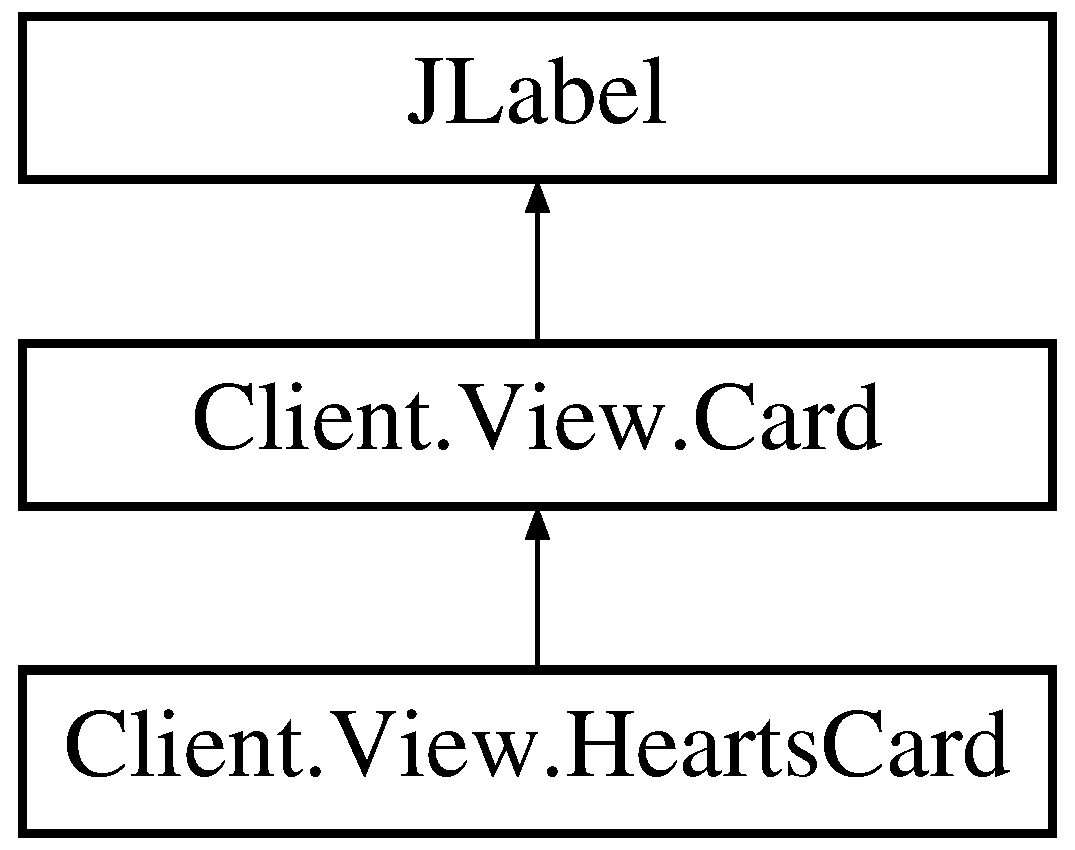
\includegraphics[height=3.000000cm]{a00048}
\end{center}
\end{figure}
\subsubsection*{Öffentliche Methoden}
\begin{DoxyCompactItemize}
\item 
\hyperlink{a00048_a6c4341c6c26359011d304a0f565484de}{Hearts\-Card} (\hyperlink{a00050}{Hearts\-I\-D} id)
\item 
\hyperlink{a00050}{Hearts\-I\-D} \hyperlink{a00048_ab8a4c181808efdbc2271fc43a732dbe4}{get\-Card\-I\-D} ()
\end{DoxyCompactItemize}


\subsubsection{Ausführliche Beschreibung}
Sie wird verwendet um einzelne Karten auf das Spielfeld zu zeichnen. Dazu enthält sie die Pfadangabe zu dem Ordner, in dem die Bilder der Karten gespeichert sind, und eine I\-D, um das genaue Bild zu spezifizieren.

\begin{DoxyAuthor}{Autor}
m4nkey 
\end{DoxyAuthor}


\subsubsection{Beschreibung der Konstruktoren und Destruktoren}
\hypertarget{a00048_a6c4341c6c26359011d304a0f565484de}{\index{Client\-::\-View\-::\-Hearts\-Card@{Client\-::\-View\-::\-Hearts\-Card}!Hearts\-Card@{Hearts\-Card}}
\index{Hearts\-Card@{Hearts\-Card}!Client::View::HeartsCard@{Client\-::\-View\-::\-Hearts\-Card}}
\paragraph[{Hearts\-Card}]{\setlength{\rightskip}{0pt plus 5cm}Client.\-View.\-Hearts\-Card.\-Hearts\-Card (
\begin{DoxyParamCaption}
\item[{{\bf Hearts\-I\-D}}]{id}
\end{DoxyParamCaption}
)}}\label{a00048_a6c4341c6c26359011d304a0f565484de}


Erstellt eine neue Hearts Karte für die Anzeige und zeichnet das Bild, das durch id spezifiziert ist. 


\begin{DoxyParams}{Parameter}
{\em id} & Hearts\-I\-D der Karte \\
\hline
\end{DoxyParams}


\subsubsection{Dokumentation der Elementfunktionen}
\hypertarget{a00048_ab8a4c181808efdbc2271fc43a732dbe4}{\index{Client\-::\-View\-::\-Hearts\-Card@{Client\-::\-View\-::\-Hearts\-Card}!get\-Card\-I\-D@{get\-Card\-I\-D}}
\index{get\-Card\-I\-D@{get\-Card\-I\-D}!Client::View::HeartsCard@{Client\-::\-View\-::\-Hearts\-Card}}
\paragraph[{get\-Card\-I\-D}]{\setlength{\rightskip}{0pt plus 5cm}{\bf Hearts\-I\-D} Client.\-View.\-Hearts\-Card.\-get\-Card\-I\-D (
\begin{DoxyParamCaption}
{}
\end{DoxyParamCaption}
)}}\label{a00048_ab8a4c181808efdbc2271fc43a732dbe4}


Gibt die Hearts\-I\-D der Karte zurück 

\begin{DoxyReturn}{Rückgabe}
Hearts\-I\-D der Karte 
\end{DoxyReturn}

\hypertarget{a00049}{\subsection{Msg\-Number\-Request Klassenreferenz}
\label{a00049}\index{Msg\-Number\-Request@{Msg\-Number\-Request}}
}


Abgeleitet von \hyperlink{a00053}{Ruleset\-Message} und Serializable.

\subsubsection*{Öffentliche Methoden}
\begin{DoxyCompactItemize}
\item 
\hypertarget{a00049_ab0f57cd806cf77f1732269ff4b4f7eee}{\hyperlink{a00049_ab0f57cd806cf77f1732269ff4b4f7eee}{Msg\-Number\-Request} ()}\label{a00049_ab0f57cd806cf77f1732269ff4b4f7eee}

\item 
void \hyperlink{a00049_ab45288da8f64e79408f1effd5579b5c2}{visit} (\hyperlink{a00068}{Server\-Ruleset} server\-Ruleset, String name)
\item 
void \hyperlink{a00049_acb5be722a2d1c9110d39f31c6e18f6e7}{visit} (\hyperlink{a00056}{Client\-Ruleset} client\-Ruleset)
\end{DoxyCompactItemize}


\subsubsection{Ausführliche Beschreibung}
Diese Klasse ist eine Verfeinerung der Ruleset\-Message-\/\-Klasse. Sie Wird gesendet, wenn die Eingabe einer Zahl gefordert werden soll. 

\subsubsection{Dokumentation der Elementfunktionen}
\hypertarget{a00049_ab45288da8f64e79408f1effd5579b5c2}{\index{Com\-Objects\-::\-Msg\-Number\-Request@{Com\-Objects\-::\-Msg\-Number\-Request}!visit@{visit}}
\index{visit@{visit}!ComObjects::MsgNumberRequest@{Com\-Objects\-::\-Msg\-Number\-Request}}
\paragraph[{visit}]{\setlength{\rightskip}{0pt plus 5cm}void visit (
\begin{DoxyParamCaption}
\item[{{\bf Server\-Ruleset}}]{server\-Ruleset, }
\item[{String}]{name}
\end{DoxyParamCaption}
)}}\label{a00049_ab45288da8f64e79408f1effd5579b5c2}


Diese Methode ist noetig, damit das Server\-Ruleset entscheiden kann welche Message es enthaelt und wie diese verarbeitet werden soll. 


\begin{DoxyParams}{Parameter}
{\em server\-Ruleset} & ist das Ruleset, welches übergeben wird, damit die ueberladene Methode richtig gewaehlt wird. \\
\hline
{\em name} & ist der Name des Spielers. \\
\hline
\end{DoxyParams}


Implementiert \hyperlink{a00053_ab45288da8f64e79408f1effd5579b5c2}{Ruleset\-Message}.

\hypertarget{a00049_acb5be722a2d1c9110d39f31c6e18f6e7}{\index{Com\-Objects\-::\-Msg\-Number\-Request@{Com\-Objects\-::\-Msg\-Number\-Request}!visit@{visit}}
\index{visit@{visit}!ComObjects::MsgNumberRequest@{Com\-Objects\-::\-Msg\-Number\-Request}}
\paragraph[{visit}]{\setlength{\rightskip}{0pt plus 5cm}void visit (
\begin{DoxyParamCaption}
\item[{{\bf Client\-Ruleset}}]{client\-Ruleset}
\end{DoxyParamCaption}
)}}\label{a00049_acb5be722a2d1c9110d39f31c6e18f6e7}


Diese Methode ist noetig, damit das Client\-Ruleset entscheiden kann welche Message es enthaelt und wie diese verarbeitet werden soll. 


\begin{DoxyParams}{Parameter}
{\em client\-Ruleset} & ist das Ruleset, welches uebergeben wird, damit die ueberladene Methode richtig gewaehlt wird. \\
\hline
\end{DoxyParams}


Implementiert \hyperlink{a00053_acb5be722a2d1c9110d39f31c6e18f6e7}{Ruleset\-Message}.


\hypertarget{a00050}{\subsection{Ruleset.\-Hearts\-I\-D Enum-\/\-Referenz}
\label{a00050}\index{Ruleset.\-Hearts\-I\-D@{Ruleset.\-Hearts\-I\-D}}
}

\hypertarget{a00051}{\subsection{Msg\-Selection\-Request Klassenreferenz}
\label{a00051}\index{Msg\-Selection\-Request@{Msg\-Selection\-Request}}
}


Abgeleitet von \hyperlink{a00053}{Ruleset\-Message} und Serializable.

\subsubsection*{Öffentliche Methoden}
\begin{DoxyCompactItemize}
\item 
\hypertarget{a00051_a1dadec1b53b67f6b1580ae0da85eb08b}{\hyperlink{a00051_a1dadec1b53b67f6b1580ae0da85eb08b}{Msg\-Selection\-Request} ()}\label{a00051_a1dadec1b53b67f6b1580ae0da85eb08b}

\item 
void \hyperlink{a00051_ab45288da8f64e79408f1effd5579b5c2}{visit} (\hyperlink{a00068}{Server\-Ruleset} server\-Ruleset, String name)
\item 
void \hyperlink{a00051_acb5be722a2d1c9110d39f31c6e18f6e7}{visit} (\hyperlink{a00056}{Client\-Ruleset} client\-Ruleset)
\end{DoxyCompactItemize}


\subsubsection{Ausführliche Beschreibung}
Diese Klasse ist eine Verfeinerung der Ruleset\-Message-\/\-Klasse. Diese Nachricht sendet der Server an einen Spieler, wenn er eine Farbauswahl von diesem erwartet. 

\subsubsection{Dokumentation der Elementfunktionen}
\hypertarget{a00051_ab45288da8f64e79408f1effd5579b5c2}{\index{Com\-Objects\-::\-Msg\-Selection\-Request@{Com\-Objects\-::\-Msg\-Selection\-Request}!visit@{visit}}
\index{visit@{visit}!ComObjects::MsgSelectionRequest@{Com\-Objects\-::\-Msg\-Selection\-Request}}
\paragraph[{visit}]{\setlength{\rightskip}{0pt plus 5cm}void visit (
\begin{DoxyParamCaption}
\item[{{\bf Server\-Ruleset}}]{server\-Ruleset, }
\item[{String}]{name}
\end{DoxyParamCaption}
)}}\label{a00051_ab45288da8f64e79408f1effd5579b5c2}


Diese Methode ist noetig, damit das Server\-Ruleset entscheiden kann welche Message es enthaelt und wie diese verarbeitet werden soll. 


\begin{DoxyParams}{Parameter}
{\em server\-Ruleset} & ist das Ruleset, welches übergeben wird, damit die ueberladene Methode richtig gewaehlt wird. \\
\hline
{\em name} & ist der Name des Spielers. \\
\hline
\end{DoxyParams}


Implementiert \hyperlink{a00053_ab45288da8f64e79408f1effd5579b5c2}{Ruleset\-Message}.

\hypertarget{a00051_acb5be722a2d1c9110d39f31c6e18f6e7}{\index{Com\-Objects\-::\-Msg\-Selection\-Request@{Com\-Objects\-::\-Msg\-Selection\-Request}!visit@{visit}}
\index{visit@{visit}!ComObjects::MsgSelectionRequest@{Com\-Objects\-::\-Msg\-Selection\-Request}}
\paragraph[{visit}]{\setlength{\rightskip}{0pt plus 5cm}void visit (
\begin{DoxyParamCaption}
\item[{{\bf Client\-Ruleset}}]{client\-Ruleset}
\end{DoxyParamCaption}
)}}\label{a00051_acb5be722a2d1c9110d39f31c6e18f6e7}


Diese Methode ist noetig, damit das Client\-Ruleset entscheiden kann welche Message es enthaelt und wie diese verarbeitet werden soll. 


\begin{DoxyParams}{Parameter}
{\em client\-Ruleset} & ist das Ruleset, welches uebergeben wird, damit die ueberladene Methode richtig gewaehlt wird. \\
\hline
\end{DoxyParams}


Implementiert \hyperlink{a00053_acb5be722a2d1c9110d39f31c6e18f6e7}{Ruleset\-Message}.


\hypertarget{a00052}{\subsection{Client.\-View.\-Language Enum-\/\-Referenz}
\label{a00052}\index{Client.\-View.\-Language@{Client.\-View.\-Language}}
}


\subsubsection{Ausführliche Beschreibung}
\begin{DoxyAuthor}{Autor}
m4nkey 
\end{DoxyAuthor}

\hypertarget{a00053}{\subsection{Ruleset\-Message Schnittstellenreferenz}
\label{a00053}\index{Ruleset\-Message@{Ruleset\-Message}}
}


Basisklasse für \hyperlink{a00043}{Msg\-Card}, \hyperlink{a00044}{Msg\-Card\-Request}, \hyperlink{a00045}{Msg\-Game\-End}, \hyperlink{a00046}{Msg\-Multi\-Cards}, \hyperlink{a00047}{Msg\-Multi\-Cards\-Request}, \hyperlink{a00048}{Msg\-Number}, \hyperlink{a00049}{Msg\-Number\-Request}, \hyperlink{a00050}{Msg\-Selection}, \hyperlink{a00051}{Msg\-Selection\-Request} und \hyperlink{a00052}{Msg\-User}.

\subsubsection*{Öffentliche Methoden}
\begin{DoxyCompactItemize}
\item 
void \hyperlink{a00053_ab45288da8f64e79408f1effd5579b5c2}{visit} (\hyperlink{a00068}{Server\-Ruleset} server\-Ruleset, String name)
\item 
void \hyperlink{a00053_acb5be722a2d1c9110d39f31c6e18f6e7}{visit} (\hyperlink{a00056}{Client\-Ruleset} client\-Ruleset)
\end{DoxyCompactItemize}


\subsubsection{Ausführliche Beschreibung}
Dieses Interface ist eine Verfeinerung der Com\-Ruleset-\/\-Klasse. Es enthaelt Methoden, die von speziellen Ruleset\-Messages implementiert werden müssen. 

\subsubsection{Dokumentation der Elementfunktionen}
\hypertarget{a00053_ab45288da8f64e79408f1effd5579b5c2}{\index{Com\-Objects\-::\-Ruleset\-Message@{Com\-Objects\-::\-Ruleset\-Message}!visit@{visit}}
\index{visit@{visit}!ComObjects::RulesetMessage@{Com\-Objects\-::\-Ruleset\-Message}}
\paragraph[{visit}]{\setlength{\rightskip}{0pt plus 5cm}void visit (
\begin{DoxyParamCaption}
\item[{{\bf Server\-Ruleset}}]{server\-Ruleset, }
\item[{String}]{name}
\end{DoxyParamCaption}
)}}\label{a00053_ab45288da8f64e79408f1effd5579b5c2}


Diese Methode ist noetig, damit das Server\-Ruleset entscheiden kann welche Message es enthaelt und wie diese verarbeitet werden soll. 


\begin{DoxyParams}{Parameter}
{\em server\-Ruleset} & ist das Ruleset, welches übergeben wird, damit die ueberladene Methode richtig gewaehlt wird. \\
\hline
{\em name} & ist der Name des Spielers. \\
\hline
\end{DoxyParams}


Implementiert in \hyperlink{a00047_ab45288da8f64e79408f1effd5579b5c2}{Msg\-Multi\-Cards\-Request}, \hyperlink{a00050_ab45288da8f64e79408f1effd5579b5c2}{Msg\-Selection}, \hyperlink{a00043_ab45288da8f64e79408f1effd5579b5c2}{Msg\-Card}, \hyperlink{a00052_ab45288da8f64e79408f1effd5579b5c2}{Msg\-User}, \hyperlink{a00045_ab45288da8f64e79408f1effd5579b5c2}{Msg\-Game\-End}, \hyperlink{a00046_ab45288da8f64e79408f1effd5579b5c2}{Msg\-Multi\-Cards}, \hyperlink{a00048_ab45288da8f64e79408f1effd5579b5c2}{Msg\-Number}, \hyperlink{a00044_ab45288da8f64e79408f1effd5579b5c2}{Msg\-Card\-Request}, \hyperlink{a00049_ab45288da8f64e79408f1effd5579b5c2}{Msg\-Number\-Request} und \hyperlink{a00051_ab45288da8f64e79408f1effd5579b5c2}{Msg\-Selection\-Request}.

\hypertarget{a00053_acb5be722a2d1c9110d39f31c6e18f6e7}{\index{Com\-Objects\-::\-Ruleset\-Message@{Com\-Objects\-::\-Ruleset\-Message}!visit@{visit}}
\index{visit@{visit}!ComObjects::RulesetMessage@{Com\-Objects\-::\-Ruleset\-Message}}
\paragraph[{visit}]{\setlength{\rightskip}{0pt plus 5cm}void visit (
\begin{DoxyParamCaption}
\item[{{\bf Client\-Ruleset}}]{client\-Ruleset}
\end{DoxyParamCaption}
)}}\label{a00053_acb5be722a2d1c9110d39f31c6e18f6e7}


Diese Methode ist noetig, damit das Client\-Ruleset entscheiden kann welche Message es enthaelt und wie diese verarbeitet werden soll. 


\begin{DoxyParams}{Parameter}
{\em client\-Ruleset} & ist das Ruleset, welches uebergeben wird, damit die ueberladene Methode richtig gewaehlt wird. \\
\hline
\end{DoxyParams}


Implementiert in \hyperlink{a00047_acb5be722a2d1c9110d39f31c6e18f6e7}{Msg\-Multi\-Cards\-Request}, \hyperlink{a00043_acb5be722a2d1c9110d39f31c6e18f6e7}{Msg\-Card}, \hyperlink{a00050_acb5be722a2d1c9110d39f31c6e18f6e7}{Msg\-Selection}, \hyperlink{a00052_acb5be722a2d1c9110d39f31c6e18f6e7}{Msg\-User}, \hyperlink{a00045_acb5be722a2d1c9110d39f31c6e18f6e7}{Msg\-Game\-End}, \hyperlink{a00046_acb5be722a2d1c9110d39f31c6e18f6e7}{Msg\-Multi\-Cards}, \hyperlink{a00048_acb5be722a2d1c9110d39f31c6e18f6e7}{Msg\-Number}, \hyperlink{a00049_acb5be722a2d1c9110d39f31c6e18f6e7}{Msg\-Number\-Request}, \hyperlink{a00051_acb5be722a2d1c9110d39f31c6e18f6e7}{Msg\-Selection\-Request} und \hyperlink{a00044_acb5be722a2d1c9110d39f31c6e18f6e7}{Msg\-Card\-Request}.


\hypertarget{a00054}{\subsection{Server.\-Lobby\-Server Klassenreferenz}
\label{a00054}\index{Server.\-Lobby\-Server@{Server.\-Lobby\-Server}}
}
Klassendiagramm für Server.\-Lobby\-Server\-:\begin{figure}[H]
\begin{center}
\leavevmode
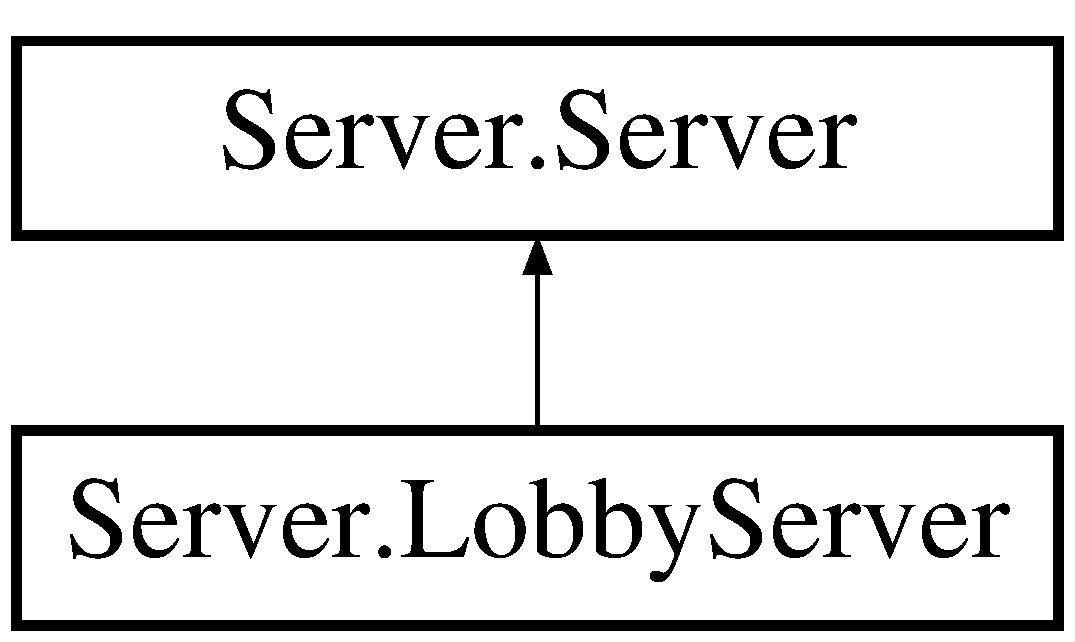
\includegraphics[height=2.000000cm]{a00054}
\end{center}
\end{figure}
\subsubsection*{Klassen}
\begin{DoxyCompactItemize}
\item 
class \hyperlink{a00011}{Client\-Listener\-Thread}
\end{DoxyCompactItemize}
\subsubsection*{Öffentliche Methoden}
\begin{DoxyCompactItemize}
\item 
void \hyperlink{a00054_ad240485402c357285d02709a08525d90}{receive\-Message} (\hyperlink{a00073}{Player} player, Com\-Chat\-Message chat)
\item 
void \hyperlink{a00054_a545d275e96d490093936496ef0c425d0}{receive\-Message} (\hyperlink{a00073}{Player} player, Com\-Client\-Quit quit)
\item 
void \hyperlink{a00054_a9c388e6df37f5c8263a4e3b54eb228ef}{receive\-Message} (\hyperlink{a00073}{Player} player, Com\-Create\-Game\-Request create)
\item 
void \hyperlink{a00054_aa636ef5ce845b8749bac73dabc5d8e74}{receive\-Message} (\hyperlink{a00073}{Player} player, Com\-Join\-Request join)
\item 
void \hyperlink{a00054_ac7ea664a020d82bb65372524a4fbeafb}{receive\-Message} (\hyperlink{a00073}{Player} player, Com\-Login\-Request login)
\item 
Com\-Init\-Lobby \hyperlink{a00054_a8f3543587bb516bbfa3cc5f3b087e3ac}{init\-Lobby} ()
\end{DoxyCompactItemize}


\subsubsection{Ausführliche Beschreibung}
Sie erstellt neue Spiele und verwaltet laufende Spiele. Auch wird der Chatverkehr über sie an die verbundenen Spieler weitergeleitet. Die Lobby\-Server-\/\-Klasse erbt Methoden zur Kommunikation vom \hyperlink{a00078}{Server}. \begin{DoxyAuthor}{Autor}
Viktoria 
\end{DoxyAuthor}


\subsubsection{Dokumentation der Elementfunktionen}
\hypertarget{a00054_a8f3543587bb516bbfa3cc5f3b087e3ac}{\index{Server\-::\-Lobby\-Server@{Server\-::\-Lobby\-Server}!init\-Lobby@{init\-Lobby}}
\index{init\-Lobby@{init\-Lobby}!Server::LobbyServer@{Server\-::\-Lobby\-Server}}
\paragraph[{init\-Lobby}]{\setlength{\rightskip}{0pt plus 5cm}Com\-Init\-Lobby Server.\-Lobby\-Server.\-init\-Lobby (
\begin{DoxyParamCaption}
{}
\end{DoxyParamCaption}
)}}\label{a00054_a8f3543587bb516bbfa3cc5f3b087e3ac}


Baut ein neues Com\-Init\-Lobby Objekt und gibt es zurück. 

\begin{DoxyReturn}{Rückgabe}
Gibt das Com\-Init\-Lobby Objekt zurück 
\end{DoxyReturn}
\hypertarget{a00054_ad240485402c357285d02709a08525d90}{\index{Server\-::\-Lobby\-Server@{Server\-::\-Lobby\-Server}!receive\-Message@{receive\-Message}}
\index{receive\-Message@{receive\-Message}!Server::LobbyServer@{Server\-::\-Lobby\-Server}}
\paragraph[{receive\-Message}]{\setlength{\rightskip}{0pt plus 5cm}void Server.\-Lobby\-Server.\-receive\-Message (
\begin{DoxyParamCaption}
\item[{{\bf Player}}]{player, }
\item[{Com\-Chat\-Message}]{chat}
\end{DoxyParamCaption}
)}}\label{a00054_ad240485402c357285d02709a08525d90}


Diese Methode ist dafür zuständig eine Chatnachricht an alle Clients im Spiel zu verschicken. 

Dafür wird die Com\-Chat\-Message mit broadcast an alle Spieler im player\-Set verteilt. 
\begin{DoxyParams}{Parameter}
{\em player} & ist der Threat der die Nachricht erhalten hat \\
\hline
{\em chat} & ist das Com\-Object, das die Chatnachricht enthält \\
\hline
\end{DoxyParams}
\hypertarget{a00054_a545d275e96d490093936496ef0c425d0}{\index{Server\-::\-Lobby\-Server@{Server\-::\-Lobby\-Server}!receive\-Message@{receive\-Message}}
\index{receive\-Message@{receive\-Message}!Server::LobbyServer@{Server\-::\-Lobby\-Server}}
\paragraph[{receive\-Message}]{\setlength{\rightskip}{0pt plus 5cm}void Server.\-Lobby\-Server.\-receive\-Message (
\begin{DoxyParamCaption}
\item[{{\bf Player}}]{player, }
\item[{Com\-Client\-Quit}]{quit}
\end{DoxyParamCaption}
)}}\label{a00054_a545d275e96d490093936496ef0c425d0}


Diese Methode schließt die Verbindung, der \hyperlink{a00073}{Player} wird aus dem player\-Set (bzw. 

no\-Names Set) entfernt, der Name des Players wird aus dem Set names entfernt. War der Spieler im player\-Set, wird ein Com\-Update\-Playerlist mit broadcast an alle Clients verschickt. 
\begin{DoxyParams}{Parameter}
{\em player} & ist der Threat der die Nachricht erhalten hat \\
\hline
{\em quit} & ist das Com\-Object, welches angibt, dass der Spieler das Spiel vollständig verlässt \\
\hline
\end{DoxyParams}
\hypertarget{a00054_a9c388e6df37f5c8263a4e3b54eb228ef}{\index{Server\-::\-Lobby\-Server@{Server\-::\-Lobby\-Server}!receive\-Message@{receive\-Message}}
\index{receive\-Message@{receive\-Message}!Server::LobbyServer@{Server\-::\-Lobby\-Server}}
\paragraph[{receive\-Message}]{\setlength{\rightskip}{0pt plus 5cm}void Server.\-Lobby\-Server.\-receive\-Message (
\begin{DoxyParamCaption}
\item[{{\bf Player}}]{player, }
\item[{Com\-Create\-Game\-Request}]{create}
\end{DoxyParamCaption}
)}}\label{a00054_a9c388e6df37f5c8263a4e3b54eb228ef}


Diese Methode erstellt einen neuen \hyperlink{a00043}{Game\-Server} fügt ihm den \hyperlink{a00073}{Player} hinzu. 

Durch broadcast wird sowohl im \hyperlink{a00054}{Lobby\-Server} als auch im \hyperlink{a00043}{Game\-Server} ein Com\-Update\-Playerlist verschickt. Zusätzlich wird dem Client mit send\-To\-Player ein Com\-Init\-Game\-Lobby geschickt. 
\begin{DoxyParams}{Parameter}
{\em player} & ist der Threat der die Nachricht erhalten hat \\
\hline
{\em create} & ist das Com\-Object, welches angibt, dass der \hyperlink{a00073}{Player} ein neues Spiel erstellt hat \\
\hline
\end{DoxyParams}
\hypertarget{a00054_aa636ef5ce845b8749bac73dabc5d8e74}{\index{Server\-::\-Lobby\-Server@{Server\-::\-Lobby\-Server}!receive\-Message@{receive\-Message}}
\index{receive\-Message@{receive\-Message}!Server::LobbyServer@{Server\-::\-Lobby\-Server}}
\paragraph[{receive\-Message}]{\setlength{\rightskip}{0pt plus 5cm}void Server.\-Lobby\-Server.\-receive\-Message (
\begin{DoxyParamCaption}
\item[{{\bf Player}}]{player, }
\item[{Com\-Join\-Request}]{join}
\end{DoxyParamCaption}
)}}\label{a00054_aa636ef5ce845b8749bac73dabc5d8e74}


Diese Methode fügt einen \hyperlink{a00073}{Player} dem entsprechenden \hyperlink{a00043}{Game\-Server} hinzu. 

Falls das Passwort nicht leer ist wird geprüft, ob es mit dem Passwort des Spieles übereinstimmt, wenn nicht, wird ein Com\-Warning an den Client geschickt. Ansonsten wird und der \hyperlink{a00073}{Player} dem, durch Namen des Spielleiters identifizierten, durch Aufruf von change\-Server Gameserver übergeben. Durch broadcast wird sowohl im \hyperlink{a00054}{Lobby\-Server} als auch im \hyperlink{a00043}{Game\-Server} ein Com\-Update\-Playerlist verschickt. Zusätzlich wird dem joinenden\-Client mit send\-To\-Player ein Com\-Init\-Game\-Lobby geschickt. 
\begin{DoxyParams}{Parameter}
{\em player} & ist der Threat der die Nachricht erhalten hat \\
\hline
{\em join} & ist das Com\-Object, welches angibt, dass der \hyperlink{a00073}{Player} einem Spiel beitreten will \\
\hline
\end{DoxyParams}
\hypertarget{a00054_ac7ea664a020d82bb65372524a4fbeafb}{\index{Server\-::\-Lobby\-Server@{Server\-::\-Lobby\-Server}!receive\-Message@{receive\-Message}}
\index{receive\-Message@{receive\-Message}!Server::LobbyServer@{Server\-::\-Lobby\-Server}}
\paragraph[{receive\-Message}]{\setlength{\rightskip}{0pt plus 5cm}void Server.\-Lobby\-Server.\-receive\-Message (
\begin{DoxyParamCaption}
\item[{{\bf Player}}]{player, }
\item[{Com\-Login\-Request}]{login}
\end{DoxyParamCaption}
)}}\label{a00054_ac7ea664a020d82bb65372524a4fbeafb}


Diese Methode überprüft, ob der Name im Set names vorhanden ist, falls ja, wird ein Com\-Warning an den Client geschickt, falls nein, wird im \hyperlink{a00073}{Player} set\-Name aufgerufen. 

Der \hyperlink{a00073}{Player} wird aus dem no\-Names Set entfernt und in das player\-Set eingefügt. Der Name wird in das Set names eingefügt. Dem Client wird ein Com\-Server\-Acknowledgement geschickt. 
\begin{DoxyParams}{Parameter}
{\em player} & ist der Threat der die Nachricht erhalten hat \\
\hline
{\em login} & ist das Com\-Object, dass den Benutzernamen des Clients enthält \\
\hline
\end{DoxyParams}

\hypertarget{a00055}{\subsection{Client\-Hearts Klassenreferenz}
\label{a00055}\index{Client\-Hearts@{Client\-Hearts}}
}


Abgeleitet von \hyperlink{a00056}{Client\-Ruleset}.

\subsubsection*{Öffentliche Methoden}
\begin{DoxyCompactItemize}
\item 
\hyperlink{a00055_ad8d72cec687ab04aa0ed6f2167b6dc33}{Client\-Hearts} (\hyperlink{a00003}{Client\-Model} \hyperlink{a00056_a937cb3d928d5cde5863e895e163b048e}{client})
\item 
boolean \hyperlink{a00055_aa58080772a961e1f9f88d766777f82ed}{is\-Valid\-Move} (\hyperlink{a00054}{Card} card)
\item 
void \hyperlink{a00055_ad32794205bdb1ca1a8760cea29d6b27a}{resolve\-Message} (\hyperlink{a00047}{Msg\-Multi\-Cards\-Request} msg\-Multi\-Cards\-Request)
\item 
boolean \hyperlink{a00055_a8f8cd3193789d852ab22bb9e858fa5c4}{are\-Valid\-Choosen\-Cards} (Set$<$ \hyperlink{a00054}{Card} $>$ cards)
\end{DoxyCompactItemize}
\subsubsection*{Statische, private Attribute}
\begin{DoxyCompactItemize}
\item 
\hypertarget{a00055_a57fe2c01c4e61b1f0c44c70ccc75d903}{static final int \hyperlink{a00055_a57fe2c01c4e61b1f0c44c70ccc75d903}{M\-I\-N\-\_\-\-P\-L\-A\-Y\-E\-R\-S} = 4}\label{a00055_a57fe2c01c4e61b1f0c44c70ccc75d903}

\item 
\hypertarget{a00055_ae6ed433235a83c520ce79bee49bc2b01}{static final int \hyperlink{a00055_ae6ed433235a83c520ce79bee49bc2b01}{M\-A\-X\-\_\-\-P\-L\-A\-Y\-E\-R\-S} = 4}\label{a00055_ae6ed433235a83c520ce79bee49bc2b01}

\item 
\hypertarget{a00055_a3045f525de18ff0ad68134f0d512ea16}{static final \hyperlink{a00066}{Ruleset\-Type} \hyperlink{a00055_a3045f525de18ff0ad68134f0d512ea16}{R\-U\-L\-E\-S\-E\-T} = \hyperlink{a00066_a6e9f988fd4b1f5b39d289b0f44514af4}{Ruleset\-Type.\-Hearts}}\label{a00055_a3045f525de18ff0ad68134f0d512ea16}

\end{DoxyCompactItemize}
\subsubsection*{Weitere Geerbte Elemente}


\subsubsection{Ausführliche Beschreibung}
Diese Klasse bildet das Regelwerk für den Clientmodel bei einer Partie Hearts 

\subsubsection{Beschreibung der Konstruktoren und Destruktoren}
\hypertarget{a00055_ad8d72cec687ab04aa0ed6f2167b6dc33}{\index{Ruleset\-::\-Client\-Hearts@{Ruleset\-::\-Client\-Hearts}!Client\-Hearts@{Client\-Hearts}}
\index{Client\-Hearts@{Client\-Hearts}!Ruleset::ClientHearts@{Ruleset\-::\-Client\-Hearts}}
\paragraph[{Client\-Hearts}]{\setlength{\rightskip}{0pt plus 5cm}{\bf Client\-Hearts} (
\begin{DoxyParamCaption}
\item[{{\bf Client\-Model}}]{client}
\end{DoxyParamCaption}
)}}\label{a00055_ad8d72cec687ab04aa0ed6f2167b6dc33}


Erzeugt ein \hyperlink{a00055}{Client\-Hearts}. 


\begin{DoxyParams}{Parameter}
{\em client} & Das Model auf dem gespielt wird \\
\hline
\end{DoxyParams}


Benutzt Ruleset\-Type.\-Hearts, Client\-Hearts.\-M\-A\-X\-\_\-\-P\-L\-A\-Y\-E\-R\-S und Client\-Hearts.\-M\-I\-N\-\_\-\-P\-L\-A\-Y\-E\-R\-S.



\subsubsection{Dokumentation der Elementfunktionen}
\hypertarget{a00055_aa58080772a961e1f9f88d766777f82ed}{\index{Ruleset\-::\-Client\-Hearts@{Ruleset\-::\-Client\-Hearts}!is\-Valid\-Move@{is\-Valid\-Move}}
\index{is\-Valid\-Move@{is\-Valid\-Move}!Ruleset::ClientHearts@{Ruleset\-::\-Client\-Hearts}}
\paragraph[{is\-Valid\-Move}]{\setlength{\rightskip}{0pt plus 5cm}boolean is\-Valid\-Move (
\begin{DoxyParamCaption}
\item[{{\bf Card}}]{card}
\end{DoxyParamCaption}
)\hspace{0.3cm}{\ttfamily [virtual]}}}\label{a00055_aa58080772a961e1f9f88d766777f82ed}


Prueft ob ein gemachter Zug in einem Spiel gueltig war. 


\begin{DoxyParams}{Parameter}
{\em card} & Die Karte \\
\hline
\end{DoxyParams}
\begin{DoxyReturn}{Rückgabe}
true falls die Karte gueltig ist, false wenn nicht 
\end{DoxyReturn}


Implementiert \hyperlink{a00056_a48cc9b97dd2832c14668fac3a6f5be1a}{Client\-Ruleset}.

\hypertarget{a00055_ad32794205bdb1ca1a8760cea29d6b27a}{\index{Ruleset\-::\-Client\-Hearts@{Ruleset\-::\-Client\-Hearts}!resolve\-Message@{resolve\-Message}}
\index{resolve\-Message@{resolve\-Message}!Ruleset::ClientHearts@{Ruleset\-::\-Client\-Hearts}}
\paragraph[{resolve\-Message}]{\setlength{\rightskip}{0pt plus 5cm}void resolve\-Message (
\begin{DoxyParamCaption}
\item[{{\bf Msg\-Multi\-Cards\-Request}}]{msg\-Multi\-Cards\-Request}
\end{DoxyParamCaption}
)}}\label{a00055_ad32794205bdb1ca1a8760cea29d6b27a}


Verarbeitet die Ruleset\-Message dass der Server von dem Spieler verlangt mehrere Karten anzugeben. 


\begin{DoxyParams}{Parameter}
{\em msg\-Multi\-Cards\-Request} & Die Nachricht vom Server \\
\hline
\end{DoxyParams}
\hypertarget{a00055_a8f8cd3193789d852ab22bb9e858fa5c4}{\index{Ruleset\-::\-Client\-Hearts@{Ruleset\-::\-Client\-Hearts}!are\-Valid\-Choosen\-Cards@{are\-Valid\-Choosen\-Cards}}
\index{are\-Valid\-Choosen\-Cards@{are\-Valid\-Choosen\-Cards}!Ruleset::ClientHearts@{Ruleset\-::\-Client\-Hearts}}
\paragraph[{are\-Valid\-Choosen\-Cards}]{\setlength{\rightskip}{0pt plus 5cm}boolean are\-Valid\-Choosen\-Cards (
\begin{DoxyParamCaption}
\item[{Set$<$ {\bf Card} $>$}]{cards}
\end{DoxyParamCaption}
)}}\label{a00055_a8f8cd3193789d852ab22bb9e858fa5c4}


Gibt zuueck ob die Karten die der Client tauschen will, gueltig sind. 


\begin{DoxyParams}{Parameter}
{\em cards} & Die zu tauschenden Karten \\
\hline
\end{DoxyParams}
\begin{DoxyReturn}{Rückgabe}
true wenn Karten valide sind, false wenn nicht 
\end{DoxyReturn}

\hypertarget{a00056}{\subsection{Client.\-Message\-Listener\-Thread Klassenreferenz}
\label{a00056}\index{Client.\-Message\-Listener\-Thread@{Client.\-Message\-Listener\-Thread}}
}

\hypertarget{a00057}{\subsection{Client\-Wizard Klassenreferenz}
\label{a00057}\index{Client\-Wizard@{Client\-Wizard}}
}


Abgeleitet von \hyperlink{a00056}{Client\-Ruleset}.

\subsubsection*{Öffentliche Methoden}
\begin{DoxyCompactItemize}
\item 
\hyperlink{a00057_a7944dd841fd8985fe49d9e2d52f36b0f}{Client\-Wizard} (\hyperlink{a00003}{Client\-Model} \hyperlink{a00056_a937cb3d928d5cde5863e895e163b048e}{client})
\item 
boolean \hyperlink{a00057_aa58080772a961e1f9f88d766777f82ed}{is\-Valid\-Move} (\hyperlink{a00054}{Card} card)
\item 
void \hyperlink{a00057_a346a9e356e52aa231aab7a309f7cf69f}{resolve\-Message} (\hyperlink{a00049}{Msg\-Number\-Request} msg\-Number)
\item 
void \hyperlink{a00057_a06db25d7d363bc633009a8722a797cc3}{resolve\-Message} (\hyperlink{a00051}{Msg\-Selection\-Request} msg\-Selection)
\item 
boolean \hyperlink{a00057_a34e8cc2994c9799ec78964834e470228}{is\-Valid\-Trick\-Number} (int number)
\item 
boolean \hyperlink{a00057_ae9116e1fb048aebeb428ffaf62599d69}{is\-Valid\-Colour} (\hyperlink{a00058}{Colour} colour)
\end{DoxyCompactItemize}
\subsubsection*{Statische, private Attribute}
\begin{DoxyCompactItemize}
\item 
\hypertarget{a00057_a57fe2c01c4e61b1f0c44c70ccc75d903}{static final int \hyperlink{a00057_a57fe2c01c4e61b1f0c44c70ccc75d903}{M\-I\-N\-\_\-\-P\-L\-A\-Y\-E\-R\-S} = 3}\label{a00057_a57fe2c01c4e61b1f0c44c70ccc75d903}

\item 
\hypertarget{a00057_ae6ed433235a83c520ce79bee49bc2b01}{static final int \hyperlink{a00057_ae6ed433235a83c520ce79bee49bc2b01}{M\-A\-X\-\_\-\-P\-L\-A\-Y\-E\-R\-S} = 6}\label{a00057_ae6ed433235a83c520ce79bee49bc2b01}

\item 
\hypertarget{a00057_a3045f525de18ff0ad68134f0d512ea16}{static final \hyperlink{a00066}{Ruleset\-Type} \hyperlink{a00057_a3045f525de18ff0ad68134f0d512ea16}{R\-U\-L\-E\-S\-E\-T} = \hyperlink{a00066_a35e49e93bdb15f20f8e9940d3f54c887}{Ruleset\-Type.\-Wizard}}\label{a00057_a3045f525de18ff0ad68134f0d512ea16}

\end{DoxyCompactItemize}
\subsubsection*{Weitere Geerbte Elemente}


\subsubsection{Ausführliche Beschreibung}
Diese Klasse bildet das Regelwerk fuer den Client bei einer Partie Wizard 

\subsubsection{Beschreibung der Konstruktoren und Destruktoren}
\hypertarget{a00057_a7944dd841fd8985fe49d9e2d52f36b0f}{\index{Ruleset\-::\-Client\-Wizard@{Ruleset\-::\-Client\-Wizard}!Client\-Wizard@{Client\-Wizard}}
\index{Client\-Wizard@{Client\-Wizard}!Ruleset::ClientWizard@{Ruleset\-::\-Client\-Wizard}}
\paragraph[{Client\-Wizard}]{\setlength{\rightskip}{0pt plus 5cm}{\bf Client\-Wizard} (
\begin{DoxyParamCaption}
\item[{{\bf Client\-Model}}]{client}
\end{DoxyParamCaption}
)}}\label{a00057_a7944dd841fd8985fe49d9e2d52f36b0f}


Erzeugt ein \hyperlink{a00057}{Client\-Wizard}. 


\begin{DoxyParams}{Parameter}
{\em client} & Das Model auf dem gespielt wird \\
\hline
\end{DoxyParams}


Benutzt Client\-Wizard.\-M\-A\-X\-\_\-\-P\-L\-A\-Y\-E\-R\-S, Client\-Wizard.\-M\-I\-N\-\_\-\-P\-L\-A\-Y\-E\-R\-S und Client\-Wizard.\-R\-U\-L\-E\-S\-E\-T.



\subsubsection{Dokumentation der Elementfunktionen}
\hypertarget{a00057_aa58080772a961e1f9f88d766777f82ed}{\index{Ruleset\-::\-Client\-Wizard@{Ruleset\-::\-Client\-Wizard}!is\-Valid\-Move@{is\-Valid\-Move}}
\index{is\-Valid\-Move@{is\-Valid\-Move}!Ruleset::ClientWizard@{Ruleset\-::\-Client\-Wizard}}
\paragraph[{is\-Valid\-Move}]{\setlength{\rightskip}{0pt plus 5cm}boolean is\-Valid\-Move (
\begin{DoxyParamCaption}
\item[{{\bf Card}}]{card}
\end{DoxyParamCaption}
)\hspace{0.3cm}{\ttfamily [virtual]}}}\label{a00057_aa58080772a961e1f9f88d766777f82ed}


Prueft ob ein gemachter Zug in einem Spiel gueltig war. 


\begin{DoxyParams}{Parameter}
{\em card} & Die Karte \\
\hline
\end{DoxyParams}
\begin{DoxyReturn}{Rückgabe}
true falls die Karte gueltig ist, false wenn nicht 
\end{DoxyReturn}


Implementiert \hyperlink{a00056_a48cc9b97dd2832c14668fac3a6f5be1a}{Client\-Ruleset}.

\hypertarget{a00057_a346a9e356e52aa231aab7a309f7cf69f}{\index{Ruleset\-::\-Client\-Wizard@{Ruleset\-::\-Client\-Wizard}!resolve\-Message@{resolve\-Message}}
\index{resolve\-Message@{resolve\-Message}!Ruleset::ClientWizard@{Ruleset\-::\-Client\-Wizard}}
\paragraph[{resolve\-Message}]{\setlength{\rightskip}{0pt plus 5cm}void resolve\-Message (
\begin{DoxyParamCaption}
\item[{{\bf Msg\-Number\-Request}}]{msg\-Number}
\end{DoxyParamCaption}
)}}\label{a00057_a346a9e356e52aa231aab7a309f7cf69f}


Verarbeitet die Ruleset\-Message dass der Server von dem Spieler verlangt eine Stichanzahl anzugeben. 


\begin{DoxyParams}{Parameter}
{\em msg\-Number} & Die Nachricht vom Server \\
\hline
\end{DoxyParams}
\hypertarget{a00057_a06db25d7d363bc633009a8722a797cc3}{\index{Ruleset\-::\-Client\-Wizard@{Ruleset\-::\-Client\-Wizard}!resolve\-Message@{resolve\-Message}}
\index{resolve\-Message@{resolve\-Message}!Ruleset::ClientWizard@{Ruleset\-::\-Client\-Wizard}}
\paragraph[{resolve\-Message}]{\setlength{\rightskip}{0pt plus 5cm}void resolve\-Message (
\begin{DoxyParamCaption}
\item[{{\bf Msg\-Selection\-Request}}]{msg\-Selection}
\end{DoxyParamCaption}
)}}\label{a00057_a06db25d7d363bc633009a8722a797cc3}


Verarbeitet die Ruleset\-Message dass der Server von dem Spieler verlangt eine Farbe auszuwählen. 


\begin{DoxyParams}{Parameter}
{\em msg\-Selection} & Die Nachricht vom Server \\
\hline
\end{DoxyParams}
\hypertarget{a00057_a34e8cc2994c9799ec78964834e470228}{\index{Ruleset\-::\-Client\-Wizard@{Ruleset\-::\-Client\-Wizard}!is\-Valid\-Trick\-Number@{is\-Valid\-Trick\-Number}}
\index{is\-Valid\-Trick\-Number@{is\-Valid\-Trick\-Number}!Ruleset::ClientWizard@{Ruleset\-::\-Client\-Wizard}}
\paragraph[{is\-Valid\-Trick\-Number}]{\setlength{\rightskip}{0pt plus 5cm}boolean is\-Valid\-Trick\-Number (
\begin{DoxyParamCaption}
\item[{int}]{number}
\end{DoxyParamCaption}
)}}\label{a00057_a34e8cc2994c9799ec78964834e470228}


Prüft ob die Anzahl der angesagten Stiche vom Spieler gültig sind. 


\begin{DoxyParams}{Parameter}
{\em number} & Die Anzahl der angesagten Sticht \\
\hline
\end{DoxyParams}
\begin{DoxyReturn}{Rückgabe}
true falls die Anzahl der Stiche passen, false wenn nicht 
\end{DoxyReturn}
\hypertarget{a00057_ae9116e1fb048aebeb428ffaf62599d69}{\index{Ruleset\-::\-Client\-Wizard@{Ruleset\-::\-Client\-Wizard}!is\-Valid\-Colour@{is\-Valid\-Colour}}
\index{is\-Valid\-Colour@{is\-Valid\-Colour}!Ruleset::ClientWizard@{Ruleset\-::\-Client\-Wizard}}
\paragraph[{is\-Valid\-Colour}]{\setlength{\rightskip}{0pt plus 5cm}boolean is\-Valid\-Colour (
\begin{DoxyParamCaption}
\item[{{\bf Colour}}]{colour}
\end{DoxyParamCaption}
)}}\label{a00057_ae9116e1fb048aebeb428ffaf62599d69}


Prüft ob die angesagte Trumpffarbe richtig. 


\begin{DoxyParams}{Parameter}
{\em colour} & Die angesagte Trumpffarbe \\
\hline
\end{DoxyParams}
\begin{DoxyReturn}{Rückgabe}
true falls die Farbe in Ordnung ist, false wenn nicht 
\end{DoxyReturn}

\hypertarget{a00058}{\subsection{Com\-Objects.\-Msg\-Card\-Request Klassenreferenz}
\label{a00058}\index{Com\-Objects.\-Msg\-Card\-Request@{Com\-Objects.\-Msg\-Card\-Request}}
}


\subsubsection{Ausführliche Beschreibung}
Diese Nachricht wird von Server gesendet, um einem Spieler mitzuteilen, dass er das Spielen einer Karte erwartet. 
\hypertarget{a00059}{\subsection{Game\-Client\-Update Klassenreferenz}
\label{a00059}\index{Game\-Client\-Update@{Game\-Client\-Update}}
}
\subsubsection*{Geschützte Methoden}
\begin{DoxyCompactItemize}
\item 
\hyperlink{a00059_a5f144c1c37887ec0dc752d035a82f031}{Game\-Client\-Update} (\hyperlink{a00065}{Player\-State} \hyperlink{a00059_a714271f36dd46095e0a17c44fdd1cbab}{player\-State}, Map$<$ String, \hyperlink{a00054}{Card} $>$ \hyperlink{a00059_abf51aa3b896825ac08fa574e68701e86}{discard\-Pile}, Map$<$ String, \hyperlink{a00064}{Other\-Data} $>$ \hyperlink{a00059_aecd7d72c15fb82c72297bfe838053122}{other\-Player\-Data}, \hyperlink{a00065}{Player\-State} \hyperlink{a00059_aa84e85401d48f310ee9959621f6c4fba}{current\-Player}, \hyperlink{a00054}{Card} \hyperlink{a00059_ab25322829797b0de34227a8e2cdb1929}{trump\-Card})
\item 
List$<$ \hyperlink{a00054}{Card} $>$ \hyperlink{a00059_a1b82d59f9b439be5785c6faffd4d3c05}{get\-Own\-Hand} ()
\item 
Map$<$ String, \hyperlink{a00054}{Card} $>$ \hyperlink{a00059_afc0981320534aa4bae54fd59dcfcad1f}{get\-Played\-Cards} ()
\item 
\hyperlink{a00064}{Other\-Data} \hyperlink{a00059_a4173e0089631ea0b571bef5965547cf6}{get\-Own\-Data} ()
\item 
\hyperlink{a00064}{Other\-Data} \hyperlink{a00059_abb320c3a473c538ecee368f8cdd4e44b}{get\-Other\-Player\-Data} (String player)
\item 
\hyperlink{a00065}{Player\-State} \hyperlink{a00059_ad3e8a11e9c53ca1b4bb6e753e48ef5ed}{get\-Current\-Player} ()
\item 
\hyperlink{a00054}{Card} \hyperlink{a00059_a278ccc7c69243be691f69d421cf7420a}{get\-Trump\-Card} ()
\end{DoxyCompactItemize}
\subsubsection*{Private Attribute}
\begin{DoxyCompactItemize}
\item 
\hypertarget{a00059_a714271f36dd46095e0a17c44fdd1cbab}{\hyperlink{a00065}{Player\-State} \hyperlink{a00059_a714271f36dd46095e0a17c44fdd1cbab}{player\-State}}\label{a00059_a714271f36dd46095e0a17c44fdd1cbab}

\item 
\hypertarget{a00059_abf51aa3b896825ac08fa574e68701e86}{Map$<$ String, \hyperlink{a00054}{Card} $>$ \hyperlink{a00059_abf51aa3b896825ac08fa574e68701e86}{discard\-Pile}}\label{a00059_abf51aa3b896825ac08fa574e68701e86}

\item 
\hypertarget{a00059_aecd7d72c15fb82c72297bfe838053122}{Map$<$ String, \hyperlink{a00064}{Other\-Data} $>$ \hyperlink{a00059_aecd7d72c15fb82c72297bfe838053122}{other\-Player\-Data}}\label{a00059_aecd7d72c15fb82c72297bfe838053122}

\item 
\hypertarget{a00059_aa84e85401d48f310ee9959621f6c4fba}{\hyperlink{a00065}{Player\-State} \hyperlink{a00059_aa84e85401d48f310ee9959621f6c4fba}{current\-Player}}\label{a00059_aa84e85401d48f310ee9959621f6c4fba}

\item 
\hypertarget{a00059_ab25322829797b0de34227a8e2cdb1929}{\hyperlink{a00054}{Card} \hyperlink{a00059_ab25322829797b0de34227a8e2cdb1929}{trump\-Card}}\label{a00059_ab25322829797b0de34227a8e2cdb1929}

\end{DoxyCompactItemize}


\subsubsection{Ausführliche Beschreibung}
Das \hyperlink{a00059}{Game\-Client\-Update} wird vom Rule\-Set ueber den Game\-Server an den Client geschickt und enthaelt alle Aenderungen des \hyperlink{a00061}{Game\-State}, die für den Client relevant sind. Das waeren seine Spielhand, der Ablagestapel sowie die Otherdata von allen Spielern und die Trumpfkarte. 

\subsubsection{Beschreibung der Konstruktoren und Destruktoren}
\hypertarget{a00059_a5f144c1c37887ec0dc752d035a82f031}{\index{Ruleset\-::\-Game\-Client\-Update@{Ruleset\-::\-Game\-Client\-Update}!Game\-Client\-Update@{Game\-Client\-Update}}
\index{Game\-Client\-Update@{Game\-Client\-Update}!Ruleset::GameClientUpdate@{Ruleset\-::\-Game\-Client\-Update}}
\paragraph[{Game\-Client\-Update}]{\setlength{\rightskip}{0pt plus 5cm}{\bf Game\-Client\-Update} (
\begin{DoxyParamCaption}
\item[{{\bf Player\-State}}]{player\-State, }
\item[{Map$<$ String, {\bf Card} $>$}]{discard\-Pile, }
\item[{Map$<$ String, {\bf Other\-Data} $>$}]{other\-Player\-Data, }
\item[{{\bf Player\-State}}]{current\-Player, }
\item[{{\bf Card}}]{trump\-Card}
\end{DoxyParamCaption}
)\hspace{0.3cm}{\ttfamily [protected]}}}\label{a00059_a5f144c1c37887ec0dc752d035a82f031}


Erstellt ein \hyperlink{a00059}{Game\-Client\-Update}. 


\begin{DoxyParams}{Parameter}
{\em player\-State} & Der Spielerzustand des Client \\
\hline
{\em discard\-Pile} & Der Ablagestapel \\
\hline
{\em other\-Player\-Data} & Die Daten der anderen Spieler \\
\hline
{\em current\-Player} & Der momentan aktive Spieler \\
\hline
{\em trump\-Card} & Die Trumpffarbe \\
\hline
\end{DoxyParams}


Benutzt Game\-Client\-Update.\-current\-Player, Game\-Client\-Update.\-discard\-Pile, Game\-Client\-Update.\-other\-Player\-Data, Game\-Client\-Update.\-player\-State und Game\-Client\-Update.\-trump\-Card.



\subsubsection{Dokumentation der Elementfunktionen}
\hypertarget{a00059_a1b82d59f9b439be5785c6faffd4d3c05}{\index{Ruleset\-::\-Game\-Client\-Update@{Ruleset\-::\-Game\-Client\-Update}!get\-Own\-Hand@{get\-Own\-Hand}}
\index{get\-Own\-Hand@{get\-Own\-Hand}!Ruleset::GameClientUpdate@{Ruleset\-::\-Game\-Client\-Update}}
\paragraph[{get\-Own\-Hand}]{\setlength{\rightskip}{0pt plus 5cm}List$<${\bf Card}$>$ get\-Own\-Hand (
\begin{DoxyParamCaption}
{}
\end{DoxyParamCaption}
)\hspace{0.3cm}{\ttfamily [protected]}}}\label{a00059_a1b82d59f9b439be5785c6faffd4d3c05}


Holt die Karten die der Client auf der Hand hat. 

\begin{DoxyReturn}{Rückgabe}
own\-Hand Die Hand des Clients 
\end{DoxyReturn}
\hypertarget{a00059_afc0981320534aa4bae54fd59dcfcad1f}{\index{Ruleset\-::\-Game\-Client\-Update@{Ruleset\-::\-Game\-Client\-Update}!get\-Played\-Cards@{get\-Played\-Cards}}
\index{get\-Played\-Cards@{get\-Played\-Cards}!Ruleset::GameClientUpdate@{Ruleset\-::\-Game\-Client\-Update}}
\paragraph[{get\-Played\-Cards}]{\setlength{\rightskip}{0pt plus 5cm}Map$<$String, {\bf Card}$>$ get\-Played\-Cards (
\begin{DoxyParamCaption}
{}
\end{DoxyParamCaption}
)\hspace{0.3cm}{\ttfamily [protected]}}}\label{a00059_afc0981320534aa4bae54fd59dcfcad1f}


Holt die gespielten Karten auf dem Ablagestapel. 

\begin{DoxyReturn}{Rückgabe}
discard\-Pile Die gespielten Karten 
\end{DoxyReturn}


Benutzt Game\-Client\-Update.\-discard\-Pile.

\hypertarget{a00059_a4173e0089631ea0b571bef5965547cf6}{\index{Ruleset\-::\-Game\-Client\-Update@{Ruleset\-::\-Game\-Client\-Update}!get\-Own\-Data@{get\-Own\-Data}}
\index{get\-Own\-Data@{get\-Own\-Data}!Ruleset::GameClientUpdate@{Ruleset\-::\-Game\-Client\-Update}}
\paragraph[{get\-Own\-Data}]{\setlength{\rightskip}{0pt plus 5cm}{\bf Other\-Data} get\-Own\-Data (
\begin{DoxyParamCaption}
{}
\end{DoxyParamCaption}
)\hspace{0.3cm}{\ttfamily [protected]}}}\label{a00059_a4173e0089631ea0b571bef5965547cf6}


Holt die Otherdata des Client als String als Stringrepräsentation. 

\begin{DoxyReturn}{Rückgabe}
own\-Data Die Otherdata des Clients 
\end{DoxyReturn}
\hypertarget{a00059_abb320c3a473c538ecee368f8cdd4e44b}{\index{Ruleset\-::\-Game\-Client\-Update@{Ruleset\-::\-Game\-Client\-Update}!get\-Other\-Player\-Data@{get\-Other\-Player\-Data}}
\index{get\-Other\-Player\-Data@{get\-Other\-Player\-Data}!Ruleset::GameClientUpdate@{Ruleset\-::\-Game\-Client\-Update}}
\paragraph[{get\-Other\-Player\-Data}]{\setlength{\rightskip}{0pt plus 5cm}{\bf Other\-Data} get\-Other\-Player\-Data (
\begin{DoxyParamCaption}
\item[{String}]{player}
\end{DoxyParamCaption}
)\hspace{0.3cm}{\ttfamily [protected]}}}\label{a00059_abb320c3a473c538ecee368f8cdd4e44b}


Holt die \hyperlink{a00064}{Other\-Data} eines anderen Spielers als Stringrepräsentation. 


\begin{DoxyParams}{Parameter}
{\em player} & Der Name des Spielers \\
\hline
\end{DoxyParams}
\begin{DoxyReturn}{Rückgabe}
other\-Player\-Data Die \hyperlink{a00064}{Other\-Data} der anderen Spieler 
\end{DoxyReturn}
\hypertarget{a00059_ad3e8a11e9c53ca1b4bb6e753e48ef5ed}{\index{Ruleset\-::\-Game\-Client\-Update@{Ruleset\-::\-Game\-Client\-Update}!get\-Current\-Player@{get\-Current\-Player}}
\index{get\-Current\-Player@{get\-Current\-Player}!Ruleset::GameClientUpdate@{Ruleset\-::\-Game\-Client\-Update}}
\paragraph[{get\-Current\-Player}]{\setlength{\rightskip}{0pt plus 5cm}{\bf Player\-State} get\-Current\-Player (
\begin{DoxyParamCaption}
{}
\end{DoxyParamCaption}
)\hspace{0.3cm}{\ttfamily [protected]}}}\label{a00059_ad3e8a11e9c53ca1b4bb6e753e48ef5ed}


Gibt den Spieler der momentan am Zug ist zurück. 

\begin{DoxyReturn}{Rückgabe}
Der momentane Spieler 
\end{DoxyReturn}


Benutzt Game\-Client\-Update.\-current\-Player.

\hypertarget{a00059_a278ccc7c69243be691f69d421cf7420a}{\index{Ruleset\-::\-Game\-Client\-Update@{Ruleset\-::\-Game\-Client\-Update}!get\-Trump\-Card@{get\-Trump\-Card}}
\index{get\-Trump\-Card@{get\-Trump\-Card}!Ruleset::GameClientUpdate@{Ruleset\-::\-Game\-Client\-Update}}
\paragraph[{get\-Trump\-Card}]{\setlength{\rightskip}{0pt plus 5cm}{\bf Card} get\-Trump\-Card (
\begin{DoxyParamCaption}
{}
\end{DoxyParamCaption}
)\hspace{0.3cm}{\ttfamily [protected]}}}\label{a00059_a278ccc7c69243be691f69d421cf7420a}


Holt die aufgedeckte Trumpfkarte. 

\begin{DoxyReturn}{Rückgabe}
trump\-Card Die Trumpfkarte 
\end{DoxyReturn}


Benutzt Game\-Client\-Update.\-trump\-Card.


\hypertarget{a00060}{\subsection{Com\-Objects.\-Msg\-Multi\-Cards Klassenreferenz}
\label{a00060}\index{Com\-Objects.\-Msg\-Multi\-Cards@{Com\-Objects.\-Msg\-Multi\-Cards}}
}
Klassendiagramm für Com\-Objects.\-Msg\-Multi\-Cards\-:\begin{figure}[H]
\begin{center}
\leavevmode
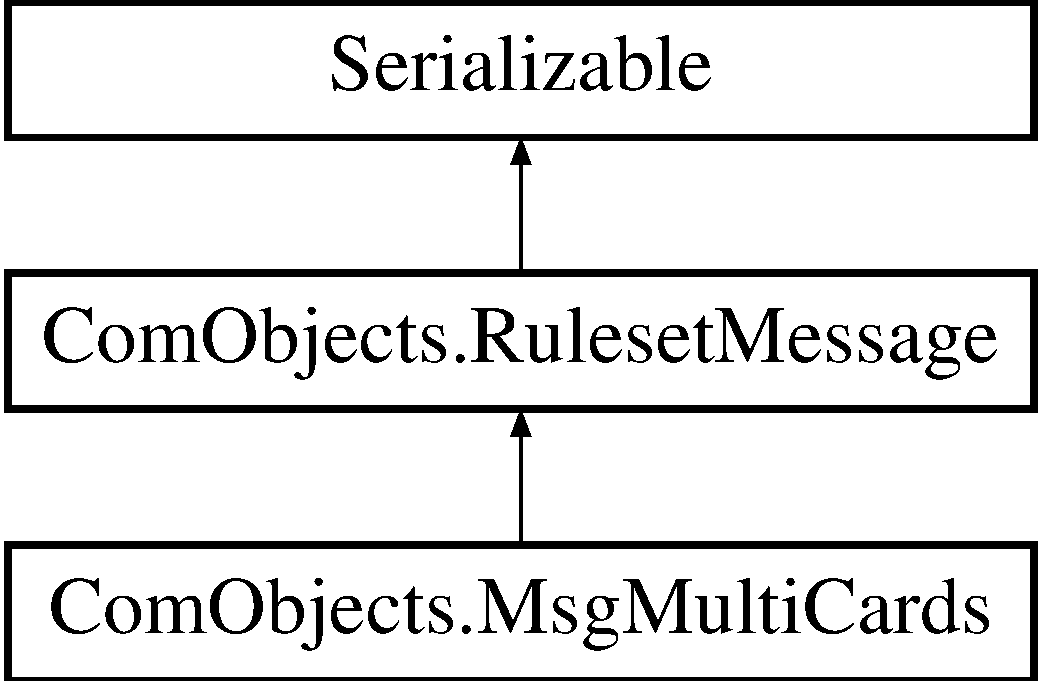
\includegraphics[height=3.000000cm]{a00060}
\end{center}
\end{figure}
\subsubsection*{Öffentliche Methoden}
\begin{DoxyCompactItemize}
\item 
\hyperlink{a00060_a1fd31dfb622bf79b9ee8672412f715a6}{Msg\-Multi\-Cards} (Set card\-List)
\item 
Set$<$ \hyperlink{a00002}{Card} $>$ \hyperlink{a00060_a9f2533083c9c59308ce69b27c19e911c}{get\-Card\-List} ()
\end{DoxyCompactItemize}


\subsubsection{Ausführliche Beschreibung}
Sie liefert mehrere Karten zum Tausch für das Regelwerk Hearts. 

\subsubsection{Beschreibung der Konstruktoren und Destruktoren}
\hypertarget{a00060_a1fd31dfb622bf79b9ee8672412f715a6}{\index{Com\-Objects\-::\-Msg\-Multi\-Cards@{Com\-Objects\-::\-Msg\-Multi\-Cards}!Msg\-Multi\-Cards@{Msg\-Multi\-Cards}}
\index{Msg\-Multi\-Cards@{Msg\-Multi\-Cards}!ComObjects::MsgMultiCards@{Com\-Objects\-::\-Msg\-Multi\-Cards}}
\paragraph[{Msg\-Multi\-Cards}]{\setlength{\rightskip}{0pt plus 5cm}Com\-Objects.\-Msg\-Multi\-Cards.\-Msg\-Multi\-Cards (
\begin{DoxyParamCaption}
\item[{Set}]{card\-List}
\end{DoxyParamCaption}
)}}\label{a00060_a1fd31dfb622bf79b9ee8672412f715a6}


Dies ist der Kontruktor für eine neue Msg\-Multi\-Cards-\/\-Nachricht. 


\begin{DoxyParams}{Parameter}
{\em card\-List} & ist die Liste der ausgewählten Karten. \\
\hline
\end{DoxyParams}


\subsubsection{Dokumentation der Elementfunktionen}
\hypertarget{a00060_a9f2533083c9c59308ce69b27c19e911c}{\index{Com\-Objects\-::\-Msg\-Multi\-Cards@{Com\-Objects\-::\-Msg\-Multi\-Cards}!get\-Card\-List@{get\-Card\-List}}
\index{get\-Card\-List@{get\-Card\-List}!ComObjects::MsgMultiCards@{Com\-Objects\-::\-Msg\-Multi\-Cards}}
\paragraph[{get\-Card\-List}]{\setlength{\rightskip}{0pt plus 5cm}Set$<${\bf Card}$>$ Com\-Objects.\-Msg\-Multi\-Cards.\-get\-Card\-List (
\begin{DoxyParamCaption}
{}
\end{DoxyParamCaption}
)}}\label{a00060_a9f2533083c9c59308ce69b27c19e911c}


Gibt die Liste der gewählten Karten zurück. 

\begin{DoxyReturn}{Rückgabe}
die Liste der Karten. 
\end{DoxyReturn}

\hypertarget{a00061}{\subsection{Com\-Objects.\-Msg\-Multi\-Cards\-Request Klassenreferenz}
\label{a00061}\index{Com\-Objects.\-Msg\-Multi\-Cards\-Request@{Com\-Objects.\-Msg\-Multi\-Cards\-Request}}
}
Klassendiagramm für Com\-Objects.\-Msg\-Multi\-Cards\-Request\-:\begin{figure}[H]
\begin{center}
\leavevmode
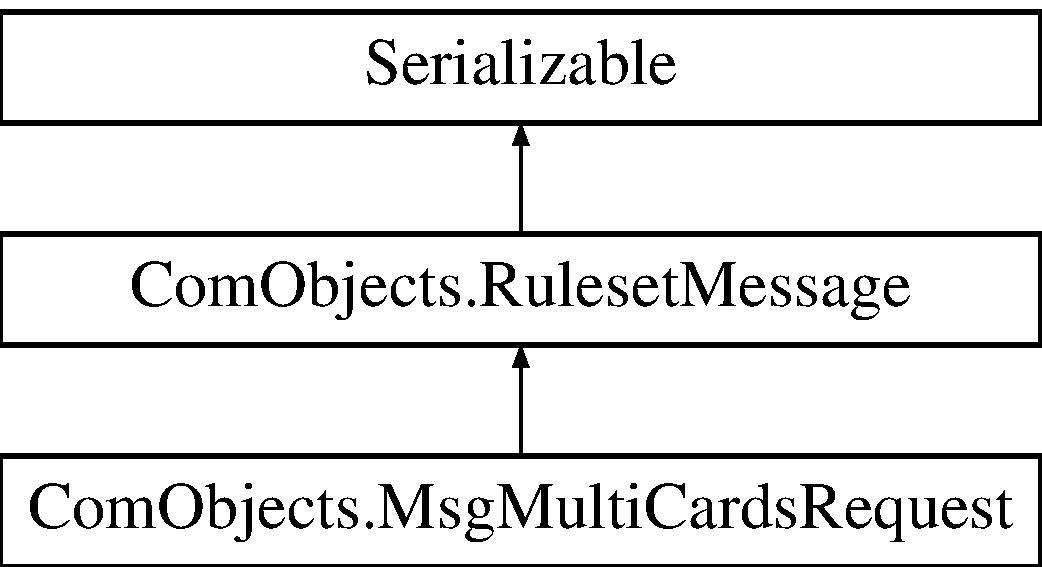
\includegraphics[height=3.000000cm]{a00061}
\end{center}
\end{figure}
\subsubsection*{Öffentliche Methoden}
\begin{DoxyCompactItemize}
\item 
int \hyperlink{a00061_ae3e54fbc631770d3abb6c2ef9b12d68f}{get\-Count} ()
\end{DoxyCompactItemize}


\subsubsection{Dokumentation der Elementfunktionen}
\hypertarget{a00061_ae3e54fbc631770d3abb6c2ef9b12d68f}{\index{Com\-Objects\-::\-Msg\-Multi\-Cards\-Request@{Com\-Objects\-::\-Msg\-Multi\-Cards\-Request}!get\-Count@{get\-Count}}
\index{get\-Count@{get\-Count}!ComObjects::MsgMultiCardsRequest@{Com\-Objects\-::\-Msg\-Multi\-Cards\-Request}}
\paragraph[{get\-Count}]{\setlength{\rightskip}{0pt plus 5cm}int Com\-Objects.\-Msg\-Multi\-Cards\-Request.\-get\-Count (
\begin{DoxyParamCaption}
{}
\end{DoxyParamCaption}
)}}\label{a00061_ae3e54fbc631770d3abb6c2ef9b12d68f}


Diese Methode gibt die Anzahl der Karten zurück, die der Server vom Spieler erwartet. 

\begin{DoxyReturn}{Rückgabe}
die Anzahl der Karten. 
\end{DoxyReturn}

\hypertarget{a00062}{\subsection{Hearts\-Card Enum-\/\-Referenz}
\label{a00062}\index{Hearts\-Card@{Hearts\-Card}}
}


Abgeleitet von \hyperlink{a00054}{Card}.

\subsubsection*{Öffentliche Methoden}
\begin{DoxyCompactItemize}
\item 
int \hyperlink{a00062_aae714dc01fe7f5bb1a175d0d1068bb92}{get\-Value} ()
\item 
\hyperlink{a00058}{Colour} \hyperlink{a00062_abdfd7d21358d1587d6383603fa77037b}{get\-Colour} ()
\end{DoxyCompactItemize}
\subsubsection*{Öffentliche Attribute}
\begin{DoxyCompactItemize}
\item 
\hypertarget{a00062_ac3e3346bc6f9bb504e43495424c91a51}{{\bfseries Empty} =(0,Colour.\-N\-O\-N\-E)}\label{a00062_ac3e3346bc6f9bb504e43495424c91a51}

\item 
\hypertarget{a00062_acb64309250e89227af937dccd161d411}{{\bfseries Herz2} =(0,Colour.\-H\-E\-A\-R\-T)}\label{a00062_acb64309250e89227af937dccd161d411}

\item 
\hypertarget{a00062_a1b9939a1f08782417119c346eca0bbc0}{{\bfseries Caro3} =(3,Colour.\-D\-I\-A\-M\-O\-N\-D)}\label{a00062_a1b9939a1f08782417119c346eca0bbc0}

\end{DoxyCompactItemize}
\subsubsection*{Private Methoden}
\begin{DoxyCompactItemize}
\item 
\hyperlink{a00062_a9a284ee50821f42af48fb03d9055c12c}{Hearts\-Card} (int \hyperlink{a00062_a899c1b74df7f8fda2fcd2c85d9185da8}{value}, \hyperlink{a00058}{Colour} \hyperlink{a00062_ad8b08a076fe1a8affe777f3f33ed8d15}{colour})
\end{DoxyCompactItemize}
\subsubsection*{Private Attribute}
\begin{DoxyCompactItemize}
\item 
\hypertarget{a00062_a899c1b74df7f8fda2fcd2c85d9185da8}{final int \hyperlink{a00062_a899c1b74df7f8fda2fcd2c85d9185da8}{value}}\label{a00062_a899c1b74df7f8fda2fcd2c85d9185da8}

\item 
\hypertarget{a00062_ad8b08a076fe1a8affe777f3f33ed8d15}{final \hyperlink{a00058}{Colour} \hyperlink{a00062_ad8b08a076fe1a8affe777f3f33ed8d15}{colour}}\label{a00062_ad8b08a076fe1a8affe777f3f33ed8d15}

\end{DoxyCompactItemize}


\subsubsection{Ausführliche Beschreibung}
Modelliert eine Heartskarte. 

\subsubsection{Beschreibung der Konstruktoren und Destruktoren}
\hypertarget{a00062_a9a284ee50821f42af48fb03d9055c12c}{\index{Ruleset\-::\-Hearts\-Card@{Ruleset\-::\-Hearts\-Card}!Hearts\-Card@{Hearts\-Card}}
\index{Hearts\-Card@{Hearts\-Card}!Ruleset::HeartsCard@{Ruleset\-::\-Hearts\-Card}}
\paragraph[{Hearts\-Card}]{\setlength{\rightskip}{0pt plus 5cm}{\bf Hearts\-Card} (
\begin{DoxyParamCaption}
\item[{int}]{value, }
\item[{{\bf Colour}}]{colour}
\end{DoxyParamCaption}
)\hspace{0.3cm}{\ttfamily [private]}}}\label{a00062_a9a284ee50821f42af48fb03d9055c12c}


Erzeugt eine Heartskarte mit einem Wert und einer Farbe. 


\begin{DoxyParams}{Parameter}
{\em value} & Der Wert der Karte \\
\hline
{\em colour} & Die Farbe der Karte \\
\hline
\end{DoxyParams}


\subsubsection{Dokumentation der Elementfunktionen}
\hypertarget{a00062_aae714dc01fe7f5bb1a175d0d1068bb92}{\index{Ruleset\-::\-Hearts\-Card@{Ruleset\-::\-Hearts\-Card}!get\-Value@{get\-Value}}
\index{get\-Value@{get\-Value}!Ruleset::HeartsCard@{Ruleset\-::\-Hearts\-Card}}
\paragraph[{get\-Value}]{\setlength{\rightskip}{0pt plus 5cm}int get\-Value (
\begin{DoxyParamCaption}
{}
\end{DoxyParamCaption}
)}}\label{a00062_aae714dc01fe7f5bb1a175d0d1068bb92}


Gibt den Wert der Karte zurück. 

\begin{DoxyReturn}{Rückgabe}
Der Wert der Karte 
\end{DoxyReturn}


Implementiert \hyperlink{a00054_aae714dc01fe7f5bb1a175d0d1068bb92}{Card}.

\hypertarget{a00062_abdfd7d21358d1587d6383603fa77037b}{\index{Ruleset\-::\-Hearts\-Card@{Ruleset\-::\-Hearts\-Card}!get\-Colour@{get\-Colour}}
\index{get\-Colour@{get\-Colour}!Ruleset::HeartsCard@{Ruleset\-::\-Hearts\-Card}}
\paragraph[{get\-Colour}]{\setlength{\rightskip}{0pt plus 5cm}{\bf Colour} get\-Colour (
\begin{DoxyParamCaption}
{}
\end{DoxyParamCaption}
)}}\label{a00062_abdfd7d21358d1587d6383603fa77037b}


Gibt die Farbe der Karte zurück. 

\begin{DoxyReturn}{Rückgabe}
Die Farbe der Karte 
\end{DoxyReturn}


Implementiert \hyperlink{a00054_abdfd7d21358d1587d6383603fa77037b}{Card}.


\hypertarget{a00063}{\subsection{Hearts\-Data Klassenreferenz}
\label{a00063}\index{Hearts\-Data@{Hearts\-Data}}
}


Abgeleitet von \hyperlink{a00064}{Other\-Data}.

\subsubsection*{Öffentliche Methoden}
\begin{DoxyCompactItemize}
\item 
\hypertarget{a00063_ad146fa8579a5f8a876c4688cc5a68520}{String \hyperlink{a00063_ad146fa8579a5f8a876c4688cc5a68520}{to\-String} ()}\label{a00063_ad146fa8579a5f8a876c4688cc5a68520}

\end{DoxyCompactItemize}
\subsubsection*{Geschützte Methoden}
\begin{DoxyCompactItemize}
\item 
\hypertarget{a00063_af0ad8b0f236fb4d365c30e384cf6b185}{\hyperlink{a00063_af0ad8b0f236fb4d365c30e384cf6b185}{Hearts\-Data} ()}\label{a00063_af0ad8b0f236fb4d365c30e384cf6b185}

\end{DoxyCompactItemize}


\subsubsection{Ausführliche Beschreibung}
Die Otherdata eines Spielers zum Spiel Hearts 
\hypertarget{a00064}{\subsection{Com\-Objects.\-Msg\-Number\-Request Klassenreferenz}
\label{a00064}\index{Com\-Objects.\-Msg\-Number\-Request@{Com\-Objects.\-Msg\-Number\-Request}}
}
Klassendiagramm für Com\-Objects.\-Msg\-Number\-Request\-:\begin{figure}[H]
\begin{center}
\leavevmode
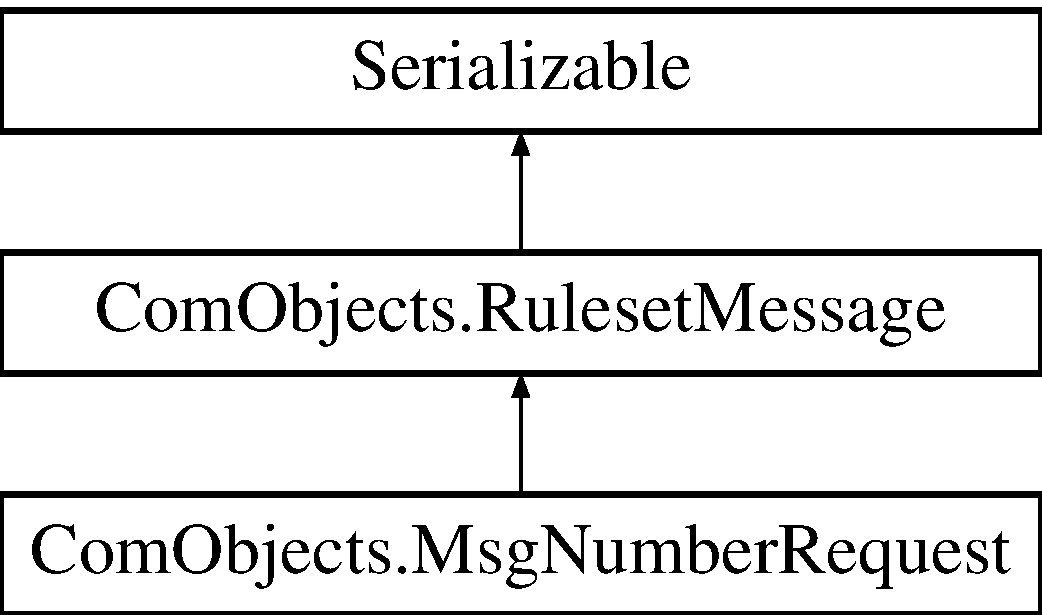
\includegraphics[height=3.000000cm]{a00064}
\end{center}
\end{figure}

\hypertarget{a00065}{\subsection{Com\-Objects.\-Msg\-Selection Klassenreferenz}
\label{a00065}\index{Com\-Objects.\-Msg\-Selection@{Com\-Objects.\-Msg\-Selection}}
}
Klassendiagramm für Com\-Objects.\-Msg\-Selection\-:\begin{figure}[H]
\begin{center}
\leavevmode
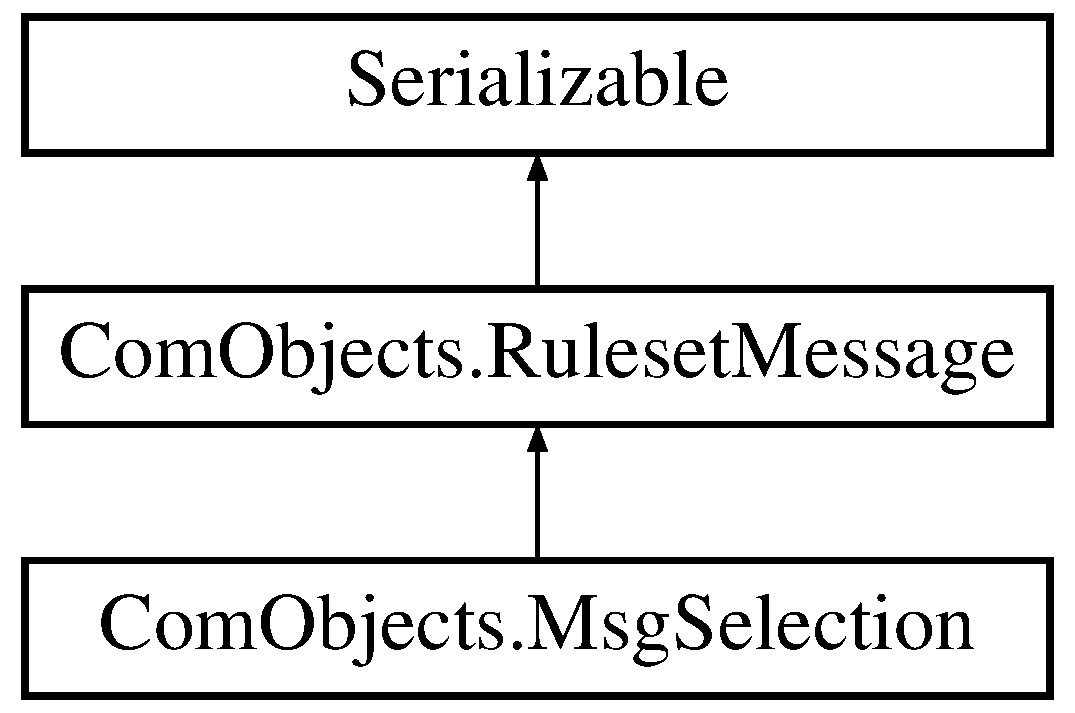
\includegraphics[height=3.000000cm]{a00065}
\end{center}
\end{figure}
\subsubsection*{Öffentliche Methoden}
\begin{DoxyCompactItemize}
\item 
\hyperlink{a00065_aaedb7500c6473ad8c880e788f4506a52}{Msg\-Selection} (int selection)
\item 
int \hyperlink{a00065_ab53c89673e153e89a1c763e786aa954e}{get\-Selection} ()
\end{DoxyCompactItemize}


\subsubsection{Ausführliche Beschreibung}
Diese Nachricht enthält Information über eine Auswahl, die der Spieler getroffen hat. Die Wahlmöglichkeiten werden durch Integer repräsentiert. 

\subsubsection{Beschreibung der Konstruktoren und Destruktoren}
\hypertarget{a00065_aaedb7500c6473ad8c880e788f4506a52}{\index{Com\-Objects\-::\-Msg\-Selection@{Com\-Objects\-::\-Msg\-Selection}!Msg\-Selection@{Msg\-Selection}}
\index{Msg\-Selection@{Msg\-Selection}!ComObjects::MsgSelection@{Com\-Objects\-::\-Msg\-Selection}}
\paragraph[{Msg\-Selection}]{\setlength{\rightskip}{0pt plus 5cm}Com\-Objects.\-Msg\-Selection.\-Msg\-Selection (
\begin{DoxyParamCaption}
\item[{int}]{selection}
\end{DoxyParamCaption}
)}}\label{a00065_aaedb7500c6473ad8c880e788f4506a52}


Dies ist der Kontruktor für eine neue Msg\-Selection-\/\-Nachricht. 


\begin{DoxyParams}{Parameter}
{\em selection} & ist die getroffene Auswahl, repräsentiert durch einen Integer. \\
\hline
\end{DoxyParams}


\subsubsection{Dokumentation der Elementfunktionen}
\hypertarget{a00065_ab53c89673e153e89a1c763e786aa954e}{\index{Com\-Objects\-::\-Msg\-Selection@{Com\-Objects\-::\-Msg\-Selection}!get\-Selection@{get\-Selection}}
\index{get\-Selection@{get\-Selection}!ComObjects::MsgSelection@{Com\-Objects\-::\-Msg\-Selection}}
\paragraph[{get\-Selection}]{\setlength{\rightskip}{0pt plus 5cm}int Com\-Objects.\-Msg\-Selection.\-get\-Selection (
\begin{DoxyParamCaption}
{}
\end{DoxyParamCaption}
)}}\label{a00065_ab53c89673e153e89a1c763e786aa954e}


Diese Methode gibt die Auswahl des Spieler zurück, die er gemacht hat. 

\begin{DoxyReturn}{Rückgabe}
die Auswahl. 
\end{DoxyReturn}

\hypertarget{a00066}{\subsection{Com\-Objects.\-Msg\-Selection\-Request Klassenreferenz}
\label{a00066}\index{Com\-Objects.\-Msg\-Selection\-Request@{Com\-Objects.\-Msg\-Selection\-Request}}
}
Klassendiagramm für Com\-Objects.\-Msg\-Selection\-Request\-:\begin{figure}[H]
\begin{center}
\leavevmode
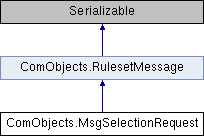
\includegraphics[height=3.000000cm]{a00066}
\end{center}
\end{figure}


\subsubsection{Ausführliche Beschreibung}
Diese Nachricht sendet der Server an einen Spieler, wenn er eine Auswahl von diesem erwartet. 
\hypertarget{a00067}{\subsection{Com\-Objects.\-Msg\-User Klassenreferenz}
\label{a00067}\index{Com\-Objects.\-Msg\-User@{Com\-Objects.\-Msg\-User}}
}
Klassendiagramm für Com\-Objects.\-Msg\-User\-:\begin{figure}[H]
\begin{center}
\leavevmode
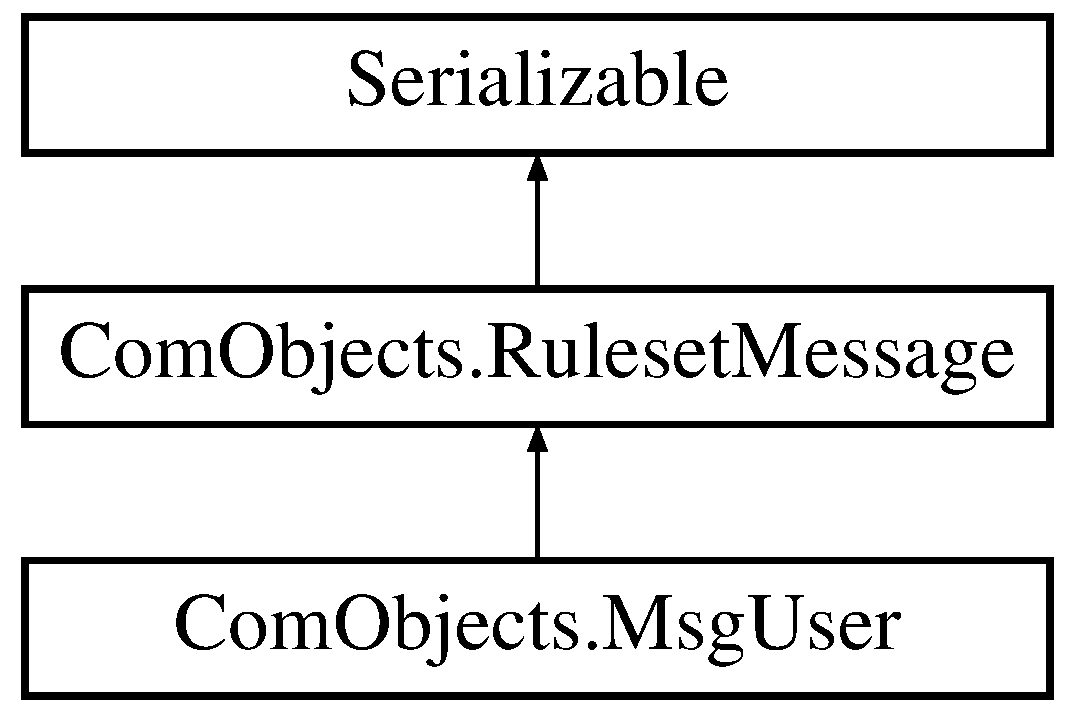
\includegraphics[height=3.000000cm]{a00067}
\end{center}
\end{figure}
\subsubsection*{Öffentliche Methoden}
\begin{DoxyCompactItemize}
\item 
\hyperlink{a00067_a031dfa573f22e616bf1f7ba7d8f8ff25}{Msg\-User} (\hyperlink{a00039}{Game\-Client\-Update} game\-Client\-Update)
\item 
\hyperlink{a00039}{Game\-Client\-Update} \hyperlink{a00067_a56b8d6525fa70a218d356c1d89b36e22}{get\-Game\-Client\-Update} ()
\end{DoxyCompactItemize}


\subsubsection{Ausführliche Beschreibung}
Sie wird dem Client gesendet, um dem Client\-Ruleset den aktuellen Spielzustand in Form eines Game\-Client\-Update zu übermitteln. 

\subsubsection{Beschreibung der Konstruktoren und Destruktoren}
\hypertarget{a00067_a031dfa573f22e616bf1f7ba7d8f8ff25}{\index{Com\-Objects\-::\-Msg\-User@{Com\-Objects\-::\-Msg\-User}!Msg\-User@{Msg\-User}}
\index{Msg\-User@{Msg\-User}!ComObjects::MsgUser@{Com\-Objects\-::\-Msg\-User}}
\paragraph[{Msg\-User}]{\setlength{\rightskip}{0pt plus 5cm}Com\-Objects.\-Msg\-User.\-Msg\-User (
\begin{DoxyParamCaption}
\item[{{\bf Game\-Client\-Update}}]{game\-Client\-Update}
\end{DoxyParamCaption}
)}}\label{a00067_a031dfa573f22e616bf1f7ba7d8f8ff25}


Dies ist der Konstruktor einer neuen Msg\-User-\/\-Nachricht. 


\begin{DoxyParams}{Parameter}
{\em game\-Client\-Update} & ist der aktuelle Spielstand. \\
\hline
\end{DoxyParams}


\subsubsection{Dokumentation der Elementfunktionen}
\hypertarget{a00067_a56b8d6525fa70a218d356c1d89b36e22}{\index{Com\-Objects\-::\-Msg\-User@{Com\-Objects\-::\-Msg\-User}!get\-Game\-Client\-Update@{get\-Game\-Client\-Update}}
\index{get\-Game\-Client\-Update@{get\-Game\-Client\-Update}!ComObjects::MsgUser@{Com\-Objects\-::\-Msg\-User}}
\paragraph[{get\-Game\-Client\-Update}]{\setlength{\rightskip}{0pt plus 5cm}{\bf Game\-Client\-Update} Com\-Objects.\-Msg\-User.\-get\-Game\-Client\-Update (
\begin{DoxyParamCaption}
{}
\end{DoxyParamCaption}
)}}\label{a00067_a56b8d6525fa70a218d356c1d89b36e22}


Diese Methode liefert den den aktuellen Spielzustand, der für ein Update benötigt wird. 

\begin{DoxyReturn}{Rückgabe}
den aktuellen Spielzustand. 
\end{DoxyReturn}

\hypertarget{a00068}{\subsection{Client.\-M\-V\-Messages Schnittstellenreferenz}
\label{a00068}\index{Client.\-M\-V\-Messages@{Client.\-M\-V\-Messages}}
}

\hypertarget{a00069}{\subsection{Server\-Wizard Klassenreferenz}
\label{a00069}\index{Server\-Wizard@{Server\-Wizard}}
}


Abgeleitet von \hyperlink{a00068}{Server\-Ruleset}.

\subsubsection*{Öffentliche Methoden}
\begin{DoxyCompactItemize}
\item 
\hypertarget{a00069_a43e18699cde5f39f7a07428c6846044c}{\hyperlink{a00069_a43e18699cde5f39f7a07428c6846044c}{Server\-Wizard} (\hyperlink{a00072}{Game\-Server} s)}\label{a00069_a43e18699cde5f39f7a07428c6846044c}

\item 
void \hyperlink{a00069_ab81696440ded730e339029a5423bd17f}{resolve\-Message} (\hyperlink{a00048}{Msg\-Number} msg\-Number, String name)
\item 
void \hyperlink{a00069_a2942b8a23a70ac5f8654690b7e3cfc09}{resolve\-Message} (\hyperlink{a00050}{Msg\-Selection} msg\-Selection, String name)
\end{DoxyCompactItemize}
\subsubsection*{Geschützte Methoden}
\begin{DoxyCompactItemize}
\item 
boolean \hyperlink{a00069_aa58080772a961e1f9f88d766777f82ed}{is\-Valid\-Move} (\hyperlink{a00054}{Card} card)
\item 
\hypertarget{a00069_aceebbbc4dd4d00fe4e4086be6acda2d7}{void \hyperlink{a00069_aceebbbc4dd4d00fe4e4086be6acda2d7}{calculate\-Round\-Outcome} ()}\label{a00069_aceebbbc4dd4d00fe4e4086be6acda2d7}

\item 
int \hyperlink{a00069_a2f51687eb56bb1a10058b2c1cc2d421e}{getplaying\-Rounds} ()
\item 
\hypertarget{a00069_a0e9e22cb0e4021e9b0fff0aa0dba1499}{void \hyperlink{a00069_a0e9e22cb0e4021e9b0fff0aa0dba1499}{calculate\-Tricks} ()}\label{a00069_a0e9e22cb0e4021e9b0fff0aa0dba1499}

\item 
\hypertarget{a00069_a159081d6eb49d67e8fe72bc03a47c336}{String \hyperlink{a00069_a159081d6eb49d67e8fe72bc03a47c336}{get\-Winner} ()}\label{a00069_a159081d6eb49d67e8fe72bc03a47c336}

\item 
\hyperlink{a00059}{Game\-Client\-Update} \hyperlink{a00069_ae26f0271bee2539ca4acd6b646ad895a}{generate\-Game\-Client\-Update} (String player)
\end{DoxyCompactItemize}
\subsubsection*{Private Methoden}
\begin{DoxyCompactItemize}
\item 
void \hyperlink{a00069_a20dac5ede6116cf0ca90930d015c4c2a}{set\-Playing\-Rounds} (int rounds)
\item 
boolean \hyperlink{a00069_a2a80072981f095510c4aeb16edc18a33}{is\-Valid\-Number} (int number, String name)
\item 
boolean \hyperlink{a00069_a5107692ee4ad56672e366f68d6714d52}{is\-Valid\-Colour} (\hyperlink{a00058}{Colour} colour, String name)
\end{DoxyCompactItemize}
\subsubsection*{Private Attribute}
\begin{DoxyCompactItemize}
\item 
int \hyperlink{a00069_afdd09d28760a65b79bafdb1551e30585}{playing\-Rounds}
\end{DoxyCompactItemize}
\subsubsection*{Statische, private Attribute}
\begin{DoxyCompactItemize}
\item 
\hypertarget{a00069_a57fe2c01c4e61b1f0c44c70ccc75d903}{static final int \hyperlink{a00069_a57fe2c01c4e61b1f0c44c70ccc75d903}{M\-I\-N\-\_\-\-P\-L\-A\-Y\-E\-R\-S} = 3}\label{a00069_a57fe2c01c4e61b1f0c44c70ccc75d903}

\item 
\hypertarget{a00069_ae6ed433235a83c520ce79bee49bc2b01}{static final int \hyperlink{a00069_ae6ed433235a83c520ce79bee49bc2b01}{M\-A\-X\-\_\-\-P\-L\-A\-Y\-E\-R\-S} = 6}\label{a00069_ae6ed433235a83c520ce79bee49bc2b01}

\item 
\hypertarget{a00069_a3045f525de18ff0ad68134f0d512ea16}{static final \hyperlink{a00066}{Ruleset\-Type} \hyperlink{a00069_a3045f525de18ff0ad68134f0d512ea16}{R\-U\-L\-E\-S\-E\-T} = \hyperlink{a00066_a35e49e93bdb15f20f8e9940d3f54c887}{Ruleset\-Type.\-Wizard}}\label{a00069_a3045f525de18ff0ad68134f0d512ea16}

\end{DoxyCompactItemize}


\subsubsection{Ausführliche Beschreibung}
Diese Klasse erstellt das Regelwerk zum Spiel Wizard. Sie enthaelt zudem weitere Methoden, welche für das Spiel Wizard spezifisch benoetigt werden, wie das Ansage von Stichen, der Bestimmung von Trumpffarben und die Bestimmung der Rundenanzahl. 

\subsubsection{Dokumentation der Elementfunktionen}
\hypertarget{a00069_aa58080772a961e1f9f88d766777f82ed}{\index{Ruleset\-::\-Server\-Wizard@{Ruleset\-::\-Server\-Wizard}!is\-Valid\-Move@{is\-Valid\-Move}}
\index{is\-Valid\-Move@{is\-Valid\-Move}!Ruleset::ServerWizard@{Ruleset\-::\-Server\-Wizard}}
\paragraph[{is\-Valid\-Move}]{\setlength{\rightskip}{0pt plus 5cm}boolean is\-Valid\-Move (
\begin{DoxyParamCaption}
\item[{{\bf Card}}]{card}
\end{DoxyParamCaption}
)\hspace{0.3cm}{\ttfamily [protected]}, {\ttfamily [virtual]}}}\label{a00069_aa58080772a961e1f9f88d766777f82ed}


Prueft ob ein gemachter Zug vom current\-Player in einem Spiel gueltig war, wenn nicht wird an den Spieler erneut eine Msg\-Card\-Request gesendet. 


\begin{DoxyParams}{Parameter}
{\em card} & Die Karte die gespielt wurde \\
\hline
\end{DoxyParams}
\begin{DoxyReturn}{Rückgabe}
true falls Zug gueltig und false wenn nicht 
\end{DoxyReturn}


Implementiert \hyperlink{a00068_a48cc9b97dd2832c14668fac3a6f5be1a}{Server\-Ruleset}.

\hypertarget{a00069_a20dac5ede6116cf0ca90930d015c4c2a}{\index{Ruleset\-::\-Server\-Wizard@{Ruleset\-::\-Server\-Wizard}!set\-Playing\-Rounds@{set\-Playing\-Rounds}}
\index{set\-Playing\-Rounds@{set\-Playing\-Rounds}!Ruleset::ServerWizard@{Ruleset\-::\-Server\-Wizard}}
\paragraph[{set\-Playing\-Rounds}]{\setlength{\rightskip}{0pt plus 5cm}void set\-Playing\-Rounds (
\begin{DoxyParamCaption}
\item[{int}]{rounds}
\end{DoxyParamCaption}
)\hspace{0.3cm}{\ttfamily [private]}}}\label{a00069_a20dac5ede6116cf0ca90930d015c4c2a}


Setzt die Anzahl an Runden die es in diesem Spiel gibt. 


\begin{DoxyParams}{Parameter}
{\em rounds} & Die Anzahl an Runden \\
\hline
\end{DoxyParams}


Benutzt Server\-Wizard.\-playing\-Rounds.

\hypertarget{a00069_a2f51687eb56bb1a10058b2c1cc2d421e}{\index{Ruleset\-::\-Server\-Wizard@{Ruleset\-::\-Server\-Wizard}!getplaying\-Rounds@{getplaying\-Rounds}}
\index{getplaying\-Rounds@{getplaying\-Rounds}!Ruleset::ServerWizard@{Ruleset\-::\-Server\-Wizard}}
\paragraph[{getplaying\-Rounds}]{\setlength{\rightskip}{0pt plus 5cm}int getplaying\-Rounds (
\begin{DoxyParamCaption}
{}
\end{DoxyParamCaption}
)\hspace{0.3cm}{\ttfamily [protected]}}}\label{a00069_a2f51687eb56bb1a10058b2c1cc2d421e}


Holt die Anzahl der Runden die gespielt werden. 

\begin{DoxyReturn}{Rückgabe}
playing\-Rounds Die Anzahl an Runden 
\end{DoxyReturn}


Benutzt Server\-Wizard.\-playing\-Rounds.

\hypertarget{a00069_ab81696440ded730e339029a5423bd17f}{\index{Ruleset\-::\-Server\-Wizard@{Ruleset\-::\-Server\-Wizard}!resolve\-Message@{resolve\-Message}}
\index{resolve\-Message@{resolve\-Message}!Ruleset::ServerWizard@{Ruleset\-::\-Server\-Wizard}}
\paragraph[{resolve\-Message}]{\setlength{\rightskip}{0pt plus 5cm}void resolve\-Message (
\begin{DoxyParamCaption}
\item[{{\bf Msg\-Number}}]{msg\-Number, }
\item[{String}]{name}
\end{DoxyParamCaption}
)}}\label{a00069_ab81696440ded730e339029a5423bd17f}


Verarbeitet die Ruleset\-Message dass der Spieler eine Stichansage macht. 

Die wird dann in is\-Valid\-Number überprüft, bei falsche Eingabe wird´ eine Msg\-Card\-Request an den selben Spieler geschickt. Bei richtiger Eingabe geht das Spiel weiter. 
\begin{DoxyParams}{Parameter}
{\em msg\-Number} & Die Nachricht vom Client \\
\hline
{\em name} & Der Name des Spielers \\
\hline
\end{DoxyParams}
\hypertarget{a00069_a2a80072981f095510c4aeb16edc18a33}{\index{Ruleset\-::\-Server\-Wizard@{Ruleset\-::\-Server\-Wizard}!is\-Valid\-Number@{is\-Valid\-Number}}
\index{is\-Valid\-Number@{is\-Valid\-Number}!Ruleset::ServerWizard@{Ruleset\-::\-Server\-Wizard}}
\paragraph[{is\-Valid\-Number}]{\setlength{\rightskip}{0pt plus 5cm}boolean is\-Valid\-Number (
\begin{DoxyParamCaption}
\item[{int}]{number, }
\item[{String}]{name}
\end{DoxyParamCaption}
)\hspace{0.3cm}{\ttfamily [private]}}}\label{a00069_a2a80072981f095510c4aeb16edc18a33}


Ueberprueft ob eine eingegebene Stichangabe eines Spielers gueltig ist. 


\begin{DoxyParams}{Parameter}
{\em number} & Die Stichangabe \\
\hline
{\em name} & Der Name vom Spieler \\
\hline
\end{DoxyParams}
\begin{DoxyReturn}{Rückgabe}
true falls die Stichangabe gültig ist, false wenn nicht 
\end{DoxyReturn}
\hypertarget{a00069_a2942b8a23a70ac5f8654690b7e3cfc09}{\index{Ruleset\-::\-Server\-Wizard@{Ruleset\-::\-Server\-Wizard}!resolve\-Message@{resolve\-Message}}
\index{resolve\-Message@{resolve\-Message}!Ruleset::ServerWizard@{Ruleset\-::\-Server\-Wizard}}
\paragraph[{resolve\-Message}]{\setlength{\rightskip}{0pt plus 5cm}void resolve\-Message (
\begin{DoxyParamCaption}
\item[{{\bf Msg\-Selection}}]{msg\-Selection, }
\item[{String}]{name}
\end{DoxyParamCaption}
)}}\label{a00069_a2942b8a23a70ac5f8654690b7e3cfc09}


Verarbeitet die Ruleset\-Message dass mehrerer Karten vom Spieler uebergeben werden. 

Die wird dann in is\-Valid\-Colour überprüft, bei falsche Eingabe wird´ Msg\-Multi\-Card\-Request an den selben Spieler geschickt. Bei richtiger Eingabe geht das Spiel weiter. 
\begin{DoxyParams}{Parameter}
{\em msg\-Selection} & Die Nachricht vom Client \\
\hline
{\em name} & Der Name des Spielers \\
\hline
\end{DoxyParams}
\hypertarget{a00069_a5107692ee4ad56672e366f68d6714d52}{\index{Ruleset\-::\-Server\-Wizard@{Ruleset\-::\-Server\-Wizard}!is\-Valid\-Colour@{is\-Valid\-Colour}}
\index{is\-Valid\-Colour@{is\-Valid\-Colour}!Ruleset::ServerWizard@{Ruleset\-::\-Server\-Wizard}}
\paragraph[{is\-Valid\-Colour}]{\setlength{\rightskip}{0pt plus 5cm}boolean is\-Valid\-Colour (
\begin{DoxyParamCaption}
\item[{{\bf Colour}}]{colour, }
\item[{String}]{name}
\end{DoxyParamCaption}
)\hspace{0.3cm}{\ttfamily [private]}}}\label{a00069_a5107692ee4ad56672e366f68d6714d52}


Ueberprueft ob eine eingebene Trumpffarbe eines Spielers gueltig ist. 


\begin{DoxyParams}{Parameter}
{\em colour} & Die Trumpffarbe \\
\hline
{\em name} & Der Name des Spielers \\
\hline
\end{DoxyParams}
\begin{DoxyReturn}{Rückgabe}
true falls die Farbe gueltig ist, false wenn nicht 
\end{DoxyReturn}
\hypertarget{a00069_ae26f0271bee2539ca4acd6b646ad895a}{\index{Ruleset\-::\-Server\-Wizard@{Ruleset\-::\-Server\-Wizard}!generate\-Game\-Client\-Update@{generate\-Game\-Client\-Update}}
\index{generate\-Game\-Client\-Update@{generate\-Game\-Client\-Update}!Ruleset::ServerWizard@{Ruleset\-::\-Server\-Wizard}}
\paragraph[{generate\-Game\-Client\-Update}]{\setlength{\rightskip}{0pt plus 5cm}{\bf Game\-Client\-Update} generate\-Game\-Client\-Update (
\begin{DoxyParamCaption}
\item[{String}]{player}
\end{DoxyParamCaption}
)\hspace{0.3cm}{\ttfamily [protected]}, {\ttfamily [virtual]}}}\label{a00069_ae26f0271bee2539ca4acd6b646ad895a}


Erzeugt ein \hyperlink{a00059}{Game\-Client\-Update} welches individuell für jeden Benutzer ist. 


\begin{DoxyParams}{Parameter}
{\em player} & Dem Spieler \\
\hline
\end{DoxyParams}


Implementiert \hyperlink{a00068_a4bc36d254178bf54e75fcdf472a5f863}{Server\-Ruleset}.



\subsubsection{Dokumentation der Datenelemente}
\hypertarget{a00069_afdd09d28760a65b79bafdb1551e30585}{\index{Ruleset\-::\-Server\-Wizard@{Ruleset\-::\-Server\-Wizard}!playing\-Rounds@{playing\-Rounds}}
\index{playing\-Rounds@{playing\-Rounds}!Ruleset::ServerWizard@{Ruleset\-::\-Server\-Wizard}}
\paragraph[{playing\-Rounds}]{\setlength{\rightskip}{0pt plus 5cm}int playing\-Rounds\hspace{0.3cm}{\ttfamily [private]}}}\label{a00069_afdd09d28760a65b79bafdb1551e30585}


Die Anzahl an Runden die gespielt wird. 

Ist abhaengig von der Spieleranzahl. 

Wird benutzt von Server\-Wizard.\-getplaying\-Rounds() und Server\-Wizard.\-set\-Playing\-Rounds().


\hypertarget{a00070}{\subsection{Client.\-View.\-Other\-Player Klassenreferenz}
\label{a00070}\index{Client.\-View.\-Other\-Player@{Client.\-View.\-Other\-Player}}
}


\subsubsection{Ausführliche Beschreibung}
\begin{DoxyAuthor}{Autor}
m4nkey 
\end{DoxyAuthor}

\hypertarget{a00071}{\subsection{Client.\-View.\-Own\-Hand Klassenreferenz}
\label{a00071}\index{Client.\-View.\-Own\-Hand@{Client.\-View.\-Own\-Hand}}
}


\subsubsection{Ausführliche Beschreibung}
Der Spieler kann eine Karte durch Anklicken auswählen und durch einen zweiten Klick ausspielen.

\begin{DoxyAuthor}{Autor}
m4nkey 
\end{DoxyAuthor}

\hypertarget{a00072}{\subsection{Client.\-View.\-Password Klassenreferenz}
\label{a00072}\index{Client.\-View.\-Password@{Client.\-View.\-Password}}
}
Klassendiagramm für Client.\-View.\-Password\-:\begin{figure}[H]
\begin{center}
\leavevmode
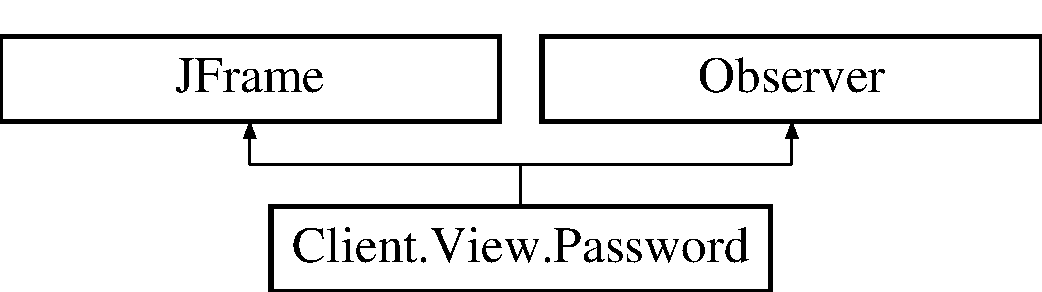
\includegraphics[height=2.000000cm]{a00072}
\end{center}
\end{figure}
\subsubsection*{Öffentliche Methoden}
\begin{DoxyCompactItemize}
\item 
void \hyperlink{a00072_aa77edfbbb4198450b8f7854b234e5365}{update} (Observable o, Object arg)
\end{DoxyCompactItemize}


\subsubsection{Ausführliche Beschreibung}
\begin{DoxyAuthor}{Autor}
M4nkey 
\end{DoxyAuthor}


\subsubsection{Dokumentation der Elementfunktionen}
\hypertarget{a00072_aa77edfbbb4198450b8f7854b234e5365}{\index{Client\-::\-View\-::\-Password@{Client\-::\-View\-::\-Password}!update@{update}}
\index{update@{update}!Client::View::Password@{Client\-::\-View\-::\-Password}}
\paragraph[{update}]{\setlength{\rightskip}{0pt plus 5cm}void Client.\-View.\-Password.\-update (
\begin{DoxyParamCaption}
\item[{Observable}]{o, }
\item[{Object}]{arg}
\end{DoxyParamCaption}
)}}\label{a00072_aa77edfbbb4198450b8f7854b234e5365}


Wird durch notify() im \hyperlink{a00013}{Client\-Model} aufgerufen. 

Je nach dem in arg �bergebenen Befehl wird ein Update des Fensters ausgef�hrt oder eine Fehlermeldung angezeigt.


\begin{DoxyParams}{Parameter}
{\em o} & erwartet ein Objekt von der Klasse \hyperlink{a00013}{Client\-Model} \\
\hline
{\em arg} & erwartet\-: window\-Change\-Acknowledged, window\-Change\-Denied \\
\hline
\end{DoxyParams}

\hypertarget{a00073}{\subsection{Server.\-Player Klassenreferenz}
\label{a00073}\index{Server.\-Player@{Server.\-Player}}
}
Klassendiagramm für Server.\-Player\-:\begin{figure}[H]
\begin{center}
\leavevmode
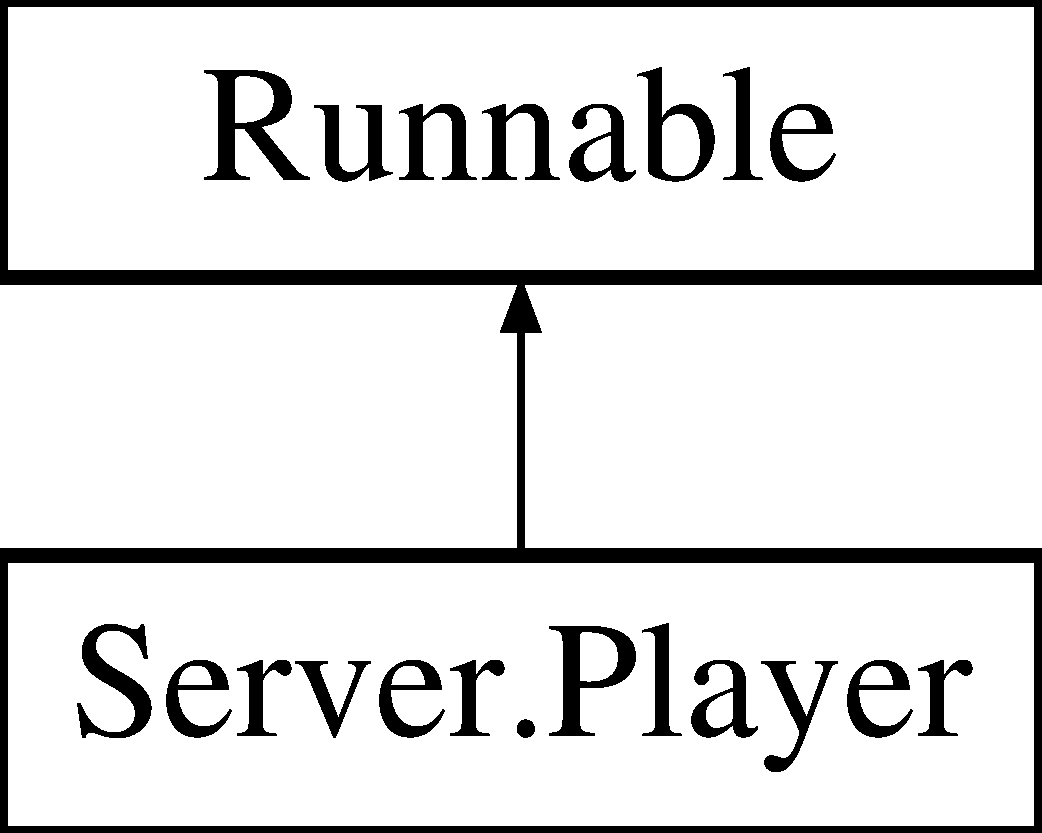
\includegraphics[height=2.000000cm]{a00073}
\end{center}
\end{figure}
\subsubsection*{Öffentliche Methoden}
\begin{DoxyCompactItemize}
\item 
\hyperlink{a00073_a858dba9ba878ab25863cad6e9b8bdbff}{Player} (\hyperlink{a00078}{Server} lobby\-Server, Object\-Output output, Object\-Input input)
\item 
void \hyperlink{a00073_aca6ecf908dbe1a01f04bf5d475c5e93d}{send} (\hyperlink{a00029}{Com\-Object} com)
\item 
void \hyperlink{a00073_a5d9f6a57cee2f22836f1ee65bf1be59c}{change\-Server} (\hyperlink{a00078}{Server} new\-Server)
\item 
String \hyperlink{a00073_ad23368a715fffac93891826bc9ec9034}{get\-Name} ()
\item 
void \hyperlink{a00073_a2ec69db14218d0d1b2ce9a2a1129b0d4}{set\-Name} (String new\-Name)
\end{DoxyCompactItemize}


\subsubsection{Ausführliche Beschreibung}
Sie verwaltet für die Dauer einer Serververbindung die Verbindung zum Client \begin{DoxyAuthor}{Autor}
Viktoria 
\end{DoxyAuthor}


\subsubsection{Beschreibung der Konstruktoren und Destruktoren}
\hypertarget{a00073_a858dba9ba878ab25863cad6e9b8bdbff}{\index{Server\-::\-Player@{Server\-::\-Player}!Player@{Player}}
\index{Player@{Player}!Server::Player@{Server\-::\-Player}}
\paragraph[{Player}]{\setlength{\rightskip}{0pt plus 5cm}Server.\-Player.\-Player (
\begin{DoxyParamCaption}
\item[{{\bf Server}}]{lobby\-Server, }
\item[{Object\-Output}]{output, }
\item[{Object\-Input}]{input}
\end{DoxyParamCaption}
)}}\label{a00073_a858dba9ba878ab25863cad6e9b8bdbff}


Konstruktor des Players, in ihm werden die Attribute server, com\-Out und Com\-In mit vom Client\-Listerer\-Thret übergebenen werten Instanziiert. 


\begin{DoxyParams}{Parameter}
{\em lobby\-Server} & ist der \hyperlink{a00054}{Lobby\-Server}, der zu Beginn den \hyperlink{a00073}{Player} verwaltet. \\
\hline
{\em output} & ist der Object\-Output an den entsprechenden Client \\
\hline
{\em input} & ist der Object\-Input vom entsprechenden Client \\
\hline
\end{DoxyParams}


\subsubsection{Dokumentation der Elementfunktionen}
\hypertarget{a00073_a5d9f6a57cee2f22836f1ee65bf1be59c}{\index{Server\-::\-Player@{Server\-::\-Player}!change\-Server@{change\-Server}}
\index{change\-Server@{change\-Server}!Server::Player@{Server\-::\-Player}}
\paragraph[{change\-Server}]{\setlength{\rightskip}{0pt plus 5cm}void Server.\-Player.\-change\-Server (
\begin{DoxyParamCaption}
\item[{{\bf Server}}]{new\-Server}
\end{DoxyParamCaption}
)}}\label{a00073_a5d9f6a57cee2f22836f1ee65bf1be59c}


Diese Methode wechselt beim \hyperlink{a00073}{Player} den \hyperlink{a00078}{Server} an den er com\-Objects weiterleiten soll. 

Dabei wird er aus dem player\-Set des alten Servers entfernt und in das player\-Set des neuen Players eingefugt. Danach wird vom neuen \hyperlink{a00078}{Server} ein Com\-Update\-Playerlist Objekt mit broadcast an alle Clients, die vom \hyperlink{a00078}{Server} verwaltet werden, verschickt. 
\begin{DoxyParams}{Parameter}
{\em new\-Server} & ist der neue \hyperlink{a00078}{Server} \\
\hline
\end{DoxyParams}
\hypertarget{a00073_ad23368a715fffac93891826bc9ec9034}{\index{Server\-::\-Player@{Server\-::\-Player}!get\-Name@{get\-Name}}
\index{get\-Name@{get\-Name}!Server::Player@{Server\-::\-Player}}
\paragraph[{get\-Name}]{\setlength{\rightskip}{0pt plus 5cm}String Server.\-Player.\-get\-Name (
\begin{DoxyParamCaption}
{}
\end{DoxyParamCaption}
)}}\label{a00073_ad23368a715fffac93891826bc9ec9034}


Getter-\/\-Methode für den Benutzernamen. 

\begin{DoxyReturn}{Rückgabe}
gibt den Benutzernamen des Spielers zurück 
\end{DoxyReturn}
\hypertarget{a00073_aca6ecf908dbe1a01f04bf5d475c5e93d}{\index{Server\-::\-Player@{Server\-::\-Player}!send@{send}}
\index{send@{send}!Server::Player@{Server\-::\-Player}}
\paragraph[{send}]{\setlength{\rightskip}{0pt plus 5cm}void Server.\-Player.\-send (
\begin{DoxyParamCaption}
\item[{{\bf Com\-Object}}]{com}
\end{DoxyParamCaption}
)}}\label{a00073_aca6ecf908dbe1a01f04bf5d475c5e93d}


Diese Methode schickt ein Com\-Objekt an den Client. 


\begin{DoxyParams}{Parameter}
{\em com} & ist das Com\-Object das verschickt wird \\
\hline
\end{DoxyParams}
\hypertarget{a00073_a2ec69db14218d0d1b2ce9a2a1129b0d4}{\index{Server\-::\-Player@{Server\-::\-Player}!set\-Name@{set\-Name}}
\index{set\-Name@{set\-Name}!Server::Player@{Server\-::\-Player}}
\paragraph[{set\-Name}]{\setlength{\rightskip}{0pt plus 5cm}void Server.\-Player.\-set\-Name (
\begin{DoxyParamCaption}
\item[{String}]{new\-Name}
\end{DoxyParamCaption}
)}}\label{a00073_a2ec69db14218d0d1b2ce9a2a1129b0d4}


Setter-\/\-Methode für den Benutzernamen. 


\begin{DoxyParams}{Parameter}
{\em new\-Name} & ist der neue Name \\
\hline
\end{DoxyParams}

\hypertarget{a00074}{\subsection{Lobby\-Server Klassenreferenz}
\label{a00074}\index{Lobby\-Server@{Lobby\-Server}}
}


Abgeleitet von \hyperlink{a00077}{Server}.

\subsubsection*{Klassen}
\begin{DoxyCompactItemize}
\item 
class \hyperlink{a00075}{Client\-Listener\-Thread}
\end{DoxyCompactItemize}
\subsubsection*{Öffentliche Methoden}
\begin{DoxyCompactItemize}
\item 
\hypertarget{a00074_a5f653627fffd8dae2f05d3200af27eb4}{\hyperlink{a00074_a5f653627fffd8dae2f05d3200af27eb4}{Lobby\-Server} ()}\label{a00074_a5f653627fffd8dae2f05d3200af27eb4}

\item 
void \hyperlink{a00074_a6cb6626c1394ab28197a8e37e438f135}{add\-Name} (String name)
\item 
void \hyperlink{a00074_a490421d42a54dd3dfeae133911b3f1ff}{remove\-Name} (String name)
\item 
void \hyperlink{a00074_a458349fade31bd4bcdcff8062e6bbe52}{add\-Game\-Server} (\hyperlink{a00072}{Game\-Server} game)
\item 
void \hyperlink{a00074_a35c0370a78b39c5af3f1eb58f42b557f}{remove\-Game\-Server} (\hyperlink{a00072}{Game\-Server} game)
\item 
void \hyperlink{a00074_a35ab43e0cc0ed85898cf687d29d79d82}{receive\-Message} (\hyperlink{a00076}{Player} player, Com\-Chat\-Message chat)
\item 
void \hyperlink{a00074_a9d96ab623d7989576a1d610ec6efe98a}{receive\-Message} (\hyperlink{a00076}{Player} player, Com\-Client\-Quit quit)
\item 
void \hyperlink{a00074_af5c4ce98894b888dbe2e2be9880251fe}{receive\-Message} (\hyperlink{a00076}{Player} player, Com\-Create\-Game\-Request create)
\item 
void \hyperlink{a00074_ab084eaa9529b43f3f78c47409c9bf506}{receive\-Message} (\hyperlink{a00076}{Player} player, Com\-Join\-Request join)
\item 
void \hyperlink{a00074_a8eb007ea65d492970bb91876da536e60}{receive\-Message} (\hyperlink{a00076}{Player} player, Com\-Login\-Request login)
\item 
Com\-Init\-Lobby \hyperlink{a00074_a93ac02d4365254caccd4388d262160df}{init\-Lobby} ()
\item 
void \hyperlink{a00074_af3ddb51daa156429385870eb04bd456e}{handle\-I\-O\-Exception} (\hyperlink{a00076}{Player} player)
\end{DoxyCompactItemize}
\subsubsection*{Private Attribute}
\begin{DoxyCompactItemize}
\item 
\hypertarget{a00074_a410d47f6c4436004d6ac20c006a7f013}{Set$<$ String $>$ \hyperlink{a00074_a410d47f6c4436004d6ac20c006a7f013}{names}}\label{a00074_a410d47f6c4436004d6ac20c006a7f013}

\item 
\hypertarget{a00074_aa01c5e296e040ef9e00462b18ec2cbb0}{Set$<$ \hyperlink{a00076}{Player} $>$ \hyperlink{a00074_aa01c5e296e040ef9e00462b18ec2cbb0}{no\-Names}}\label{a00074_aa01c5e296e040ef9e00462b18ec2cbb0}

\item 
\hypertarget{a00074_a50829648a03f89348ae5d37a256aed98}{Set$<$ \hyperlink{a00072}{Game\-Server} $>$ \hyperlink{a00074_a50829648a03f89348ae5d37a256aed98}{game\-Server\-Set}}\label{a00074_a50829648a03f89348ae5d37a256aed98}

\item 
\hypertarget{a00074_aea765ab1affc1ca4aa581e91fe4dbf56}{\hyperlink{a00075}{Client\-Listener\-Thread} \hyperlink{a00074_aea765ab1affc1ca4aa581e91fe4dbf56}{client\-Listener\-Thread}}\label{a00074_aea765ab1affc1ca4aa581e91fe4dbf56}

\item 
\hypertarget{a00074_a7c2dae918c1b5f03cf1b5a7adb972529}{Server\-Socket \hyperlink{a00074_a7c2dae918c1b5f03cf1b5a7adb972529}{socket}}\label{a00074_a7c2dae918c1b5f03cf1b5a7adb972529}

\end{DoxyCompactItemize}
\subsubsection*{Weitere Geerbte Elemente}


\subsubsection{Ausführliche Beschreibung}
Diese Klasse ist fuer die Verwaltung der Spiellobby auf dem \hyperlink{a00077}{Server} verantwortlich. Sie erstellt neue Spiele und verwaltet laufende Spiele. Auch wird der Chatverkehr ueber sie an die verbundenen Spieler weitergeleitet. Die Lobby\-Server-\/\-Klasse erbt Methoden zur Kommunikation vom \hyperlink{a00077}{Server}. 

\subsubsection{Dokumentation der Elementfunktionen}
\hypertarget{a00074_a6cb6626c1394ab28197a8e37e438f135}{\index{Server\-::\-Lobby\-Server@{Server\-::\-Lobby\-Server}!add\-Name@{add\-Name}}
\index{add\-Name@{add\-Name}!Server::LobbyServer@{Server\-::\-Lobby\-Server}}
\paragraph[{add\-Name}]{\setlength{\rightskip}{0pt plus 5cm}void add\-Name (
\begin{DoxyParamCaption}
\item[{String}]{name}
\end{DoxyParamCaption}
)}}\label{a00074_a6cb6626c1394ab28197a8e37e438f135}


Fuegt einen neuen Benutzennamen in das Namensset ein. 

Es wird vorrausgesetzt, dass der Name noch nicht im Set vorhanden ist. 
\begin{DoxyParams}{Parameter}
{\em name} & ist der Name der eingefuegt wird \\
\hline
\end{DoxyParams}
\hypertarget{a00074_a490421d42a54dd3dfeae133911b3f1ff}{\index{Server\-::\-Lobby\-Server@{Server\-::\-Lobby\-Server}!remove\-Name@{remove\-Name}}
\index{remove\-Name@{remove\-Name}!Server::LobbyServer@{Server\-::\-Lobby\-Server}}
\paragraph[{remove\-Name}]{\setlength{\rightskip}{0pt plus 5cm}void remove\-Name (
\begin{DoxyParamCaption}
\item[{String}]{name}
\end{DoxyParamCaption}
)}}\label{a00074_a490421d42a54dd3dfeae133911b3f1ff}


Loescht einen Benutzennamen aus dem Namensset. 

Es wird vorrausgesetzt, dass der Name im Set vorhanden ist. 
\begin{DoxyParams}{Parameter}
{\em name} & ist der Name der geloescht wird \\
\hline
\end{DoxyParams}
\hypertarget{a00074_a458349fade31bd4bcdcff8062e6bbe52}{\index{Server\-::\-Lobby\-Server@{Server\-::\-Lobby\-Server}!add\-Game\-Server@{add\-Game\-Server}}
\index{add\-Game\-Server@{add\-Game\-Server}!Server::LobbyServer@{Server\-::\-Lobby\-Server}}
\paragraph[{add\-Game\-Server}]{\setlength{\rightskip}{0pt plus 5cm}void add\-Game\-Server (
\begin{DoxyParamCaption}
\item[{{\bf Game\-Server}}]{game}
\end{DoxyParamCaption}
)}}\label{a00074_a458349fade31bd4bcdcff8062e6bbe52}


Fuegt einen neuen \hyperlink{a00072}{Game\-Server} in das game\-Server\-Set ein. 


\begin{DoxyParams}{Parameter}
{\em game} & ist der \hyperlink{a00072}{Game\-Server} der eingefuegt wird \\
\hline
\end{DoxyParams}
\hypertarget{a00074_a35c0370a78b39c5af3f1eb58f42b557f}{\index{Server\-::\-Lobby\-Server@{Server\-::\-Lobby\-Server}!remove\-Game\-Server@{remove\-Game\-Server}}
\index{remove\-Game\-Server@{remove\-Game\-Server}!Server::LobbyServer@{Server\-::\-Lobby\-Server}}
\paragraph[{remove\-Game\-Server}]{\setlength{\rightskip}{0pt plus 5cm}void remove\-Game\-Server (
\begin{DoxyParamCaption}
\item[{{\bf Game\-Server}}]{game}
\end{DoxyParamCaption}
)}}\label{a00074_a35c0370a78b39c5af3f1eb58f42b557f}


Loescht einen \hyperlink{a00072}{Game\-Server} aus dem Gameserverset. 


\begin{DoxyParams}{Parameter}
{\em game} & ist der \hyperlink{a00072}{Game\-Server} der geloescht wird \\
\hline
\end{DoxyParams}
\hypertarget{a00074_a35ab43e0cc0ed85898cf687d29d79d82}{\index{Server\-::\-Lobby\-Server@{Server\-::\-Lobby\-Server}!receive\-Message@{receive\-Message}}
\index{receive\-Message@{receive\-Message}!Server::LobbyServer@{Server\-::\-Lobby\-Server}}
\paragraph[{receive\-Message}]{\setlength{\rightskip}{0pt plus 5cm}void receive\-Message (
\begin{DoxyParamCaption}
\item[{{\bf Player}}]{player, }
\item[{Com\-Chat\-Message}]{chat}
\end{DoxyParamCaption}
)}}\label{a00074_a35ab43e0cc0ed85898cf687d29d79d82}


Diese ueberladene Methode ist dafuer zustaendig eine Chatnachricht an alle Clients im Spiel zu verschicken. 

Dafuer wird die Com\-Chat\-Message mit broadcast an alle Spieler im player\-Set verteilt. 
\begin{DoxyParams}{Parameter}
{\em player} & ist der Thread der die Nachricht erhalten hat \\
\hline
{\em chat} & ist das Com\-Object, das die Chatnachricht enthaelt \\
\hline
\end{DoxyParams}


Benutzt Server.\-broadcast().

\hypertarget{a00074_a9d96ab623d7989576a1d610ec6efe98a}{\index{Server\-::\-Lobby\-Server@{Server\-::\-Lobby\-Server}!receive\-Message@{receive\-Message}}
\index{receive\-Message@{receive\-Message}!Server::LobbyServer@{Server\-::\-Lobby\-Server}}
\paragraph[{receive\-Message}]{\setlength{\rightskip}{0pt plus 5cm}void receive\-Message (
\begin{DoxyParamCaption}
\item[{{\bf Player}}]{player, }
\item[{Com\-Client\-Quit}]{quit}
\end{DoxyParamCaption}
)}}\label{a00074_a9d96ab623d7989576a1d610ec6efe98a}


Diese ueberladene Methode schliesst die Verbindung, der \hyperlink{a00076}{Player} wird aus dem player\-Set (bzw. 

no\-Names Set) entfernt, der Name des Players wird aus dem Set names entfernt. War der Spieler im player\-Set, wird ein Com\-Update\-Playerlist mit broadcast an alle Clients verschickt. 
\begin{DoxyParams}{Parameter}
{\em player} & ist der Thread der die Nachricht erhalten hat \\
\hline
{\em quit} & ist das Com\-Object, welches angibt, dass der Spieler das Spiel vollstaendig verlaesst \\
\hline
\end{DoxyParams}
\hypertarget{a00074_af5c4ce98894b888dbe2e2be9880251fe}{\index{Server\-::\-Lobby\-Server@{Server\-::\-Lobby\-Server}!receive\-Message@{receive\-Message}}
\index{receive\-Message@{receive\-Message}!Server::LobbyServer@{Server\-::\-Lobby\-Server}}
\paragraph[{receive\-Message}]{\setlength{\rightskip}{0pt plus 5cm}void receive\-Message (
\begin{DoxyParamCaption}
\item[{{\bf Player}}]{player, }
\item[{Com\-Create\-Game\-Request}]{create}
\end{DoxyParamCaption}
)}}\label{a00074_af5c4ce98894b888dbe2e2be9880251fe}


Diese ueberladene Methode erstellt einen neuen \hyperlink{a00072}{Game\-Server} fuegt ihm den \hyperlink{a00076}{Player} durch Aufruf von dessen change\-Server Methode hinzu. 

Der neue \hyperlink{a00072}{Game\-Server} wird in das game\-Server\-Set eingefuegt. Durch broadcast wird im \hyperlink{a00074}{Lobby\-Server} sowohl Com\-Update\-Playerlist als auch ein Com\-Lobby\-Update\-Gamelist verschickt. Zusaetzlich wird dem Client mit send\-To\-Player ein Com\-Init\-Game\-Lobby geschickt. 
\begin{DoxyParams}{Parameter}
{\em player} & ist der Thread der die Nachricht erhalten hat \\
\hline
{\em create} & ist das Com\-Object, welches angibt, dass der \hyperlink{a00076}{Player} ein neues Spiel erstellt hat \\
\hline
\end{DoxyParams}
\hypertarget{a00074_ab084eaa9529b43f3f78c47409c9bf506}{\index{Server\-::\-Lobby\-Server@{Server\-::\-Lobby\-Server}!receive\-Message@{receive\-Message}}
\index{receive\-Message@{receive\-Message}!Server::LobbyServer@{Server\-::\-Lobby\-Server}}
\paragraph[{receive\-Message}]{\setlength{\rightskip}{0pt plus 5cm}void receive\-Message (
\begin{DoxyParamCaption}
\item[{{\bf Player}}]{player, }
\item[{Com\-Join\-Request}]{join}
\end{DoxyParamCaption}
)}}\label{a00074_ab084eaa9529b43f3f78c47409c9bf506}


Diese ueberladene Methode fuegt einen \hyperlink{a00076}{Player} dem entsprechenden \hyperlink{a00072}{Game\-Server} hinzu. 

Falls das Passwort nicht leer ist wird geprueft, ob es mit dem Passwort des Spieles uebereinstimmt, wenn nicht, wird ein Com\-Warning an den Client geschickt. Ansonsten wird und der \hyperlink{a00076}{Player} dem, durch Namen des Spielleiters identifizierten, Gameserver, durch Aufruf von change\-Server uebergeben. Dem joinenden\-Client wird mit send\-To\-Player ein Com\-Init\-Game\-Lobby geschickt. Durch broadcast wird sowohl im \hyperlink{a00074}{Lobby\-Server} ein Com\-Update\-Playerlist verschickt. 
\begin{DoxyParams}{Parameter}
{\em player} & ist der Thread der die Nachricht erhalten hat \\
\hline
{\em join} & ist das Com\-Object, welches angibt, dass der \hyperlink{a00076}{Player} einem Spiel beitreten will \\
\hline
\end{DoxyParams}
\hypertarget{a00074_a8eb007ea65d492970bb91876da536e60}{\index{Server\-::\-Lobby\-Server@{Server\-::\-Lobby\-Server}!receive\-Message@{receive\-Message}}
\index{receive\-Message@{receive\-Message}!Server::LobbyServer@{Server\-::\-Lobby\-Server}}
\paragraph[{receive\-Message}]{\setlength{\rightskip}{0pt plus 5cm}void receive\-Message (
\begin{DoxyParamCaption}
\item[{{\bf Player}}]{player, }
\item[{Com\-Login\-Request}]{login}
\end{DoxyParamCaption}
)}}\label{a00074_a8eb007ea65d492970bb91876da536e60}


Diese ueberladene Methode ueberprueft, ob der Name im Set names vorhanden ist, falls ja, wird ein Com\-Warning an den Client geschickt, dass der Name bereits vergeben ist, falls nein, wird im \hyperlink{a00076}{Player} set\-Name aufgerufen. 

Der \hyperlink{a00076}{Player} wird aus dem no\-Names Set entfernt und in das player\-Set eingefuegt. Der Name wird in das Set names eingefuegt. Dem Client wird ein Com\-Server\-Acknowledgement geschickt. 
\begin{DoxyParams}{Parameter}
{\em player} & ist der Thread der die Nachricht erhalten hat \\
\hline
{\em login} & ist das Com\-Object, dass den Benutzernamen des Clients enthält \\
\hline
\end{DoxyParams}
\hypertarget{a00074_a93ac02d4365254caccd4388d262160df}{\index{Server\-::\-Lobby\-Server@{Server\-::\-Lobby\-Server}!init\-Lobby@{init\-Lobby}}
\index{init\-Lobby@{init\-Lobby}!Server::LobbyServer@{Server\-::\-Lobby\-Server}}
\paragraph[{init\-Lobby}]{\setlength{\rightskip}{0pt plus 5cm}Com\-Init\-Lobby init\-Lobby (
\begin{DoxyParamCaption}
{}
\end{DoxyParamCaption}
)}}\label{a00074_a93ac02d4365254caccd4388d262160df}


Diese Methode baut ein neues Com\-Init\-Lobby Objekt und gibt es zurueck. 

\begin{DoxyReturn}{Rückgabe}
Gibt das Com\-Init\-Lobby Objekt zurueck 
\end{DoxyReturn}
\hypertarget{a00074_af3ddb51daa156429385870eb04bd456e}{\index{Server\-::\-Lobby\-Server@{Server\-::\-Lobby\-Server}!handle\-I\-O\-Exception@{handle\-I\-O\-Exception}}
\index{handle\-I\-O\-Exception@{handle\-I\-O\-Exception}!Server::LobbyServer@{Server\-::\-Lobby\-Server}}
\paragraph[{handle\-I\-O\-Exception}]{\setlength{\rightskip}{0pt plus 5cm}void handle\-I\-O\-Exception (
\begin{DoxyParamCaption}
\item[{{\bf Player}}]{player}
\end{DoxyParamCaption}
)}}\label{a00074_af3ddb51daa156429385870eb04bd456e}


Diese Methode legt den Ablauf fest, was passiert, falls die Verbindung zu einem Client verloren gegangen ist. 

Der uebergebene \hyperlink{a00076}{Player} wird aus dem player\-Set sowie dem names Set im \hyperlink{a00074}{Lobby\-Server} entfernt. 
\begin{DoxyParams}{Parameter}
{\em player} & ist der Tread von dem die I\-O\-Exception kommt \\
\hline
\end{DoxyParams}

\hypertarget{a00075}{\subsection{Com\-Objects.\-Ruleset\-Message Klassenreferenz}
\label{a00075}\index{Com\-Objects.\-Ruleset\-Message@{Com\-Objects.\-Ruleset\-Message}}
}
Klassendiagramm für Com\-Objects.\-Ruleset\-Message\-:\begin{figure}[H]
\begin{center}
\leavevmode
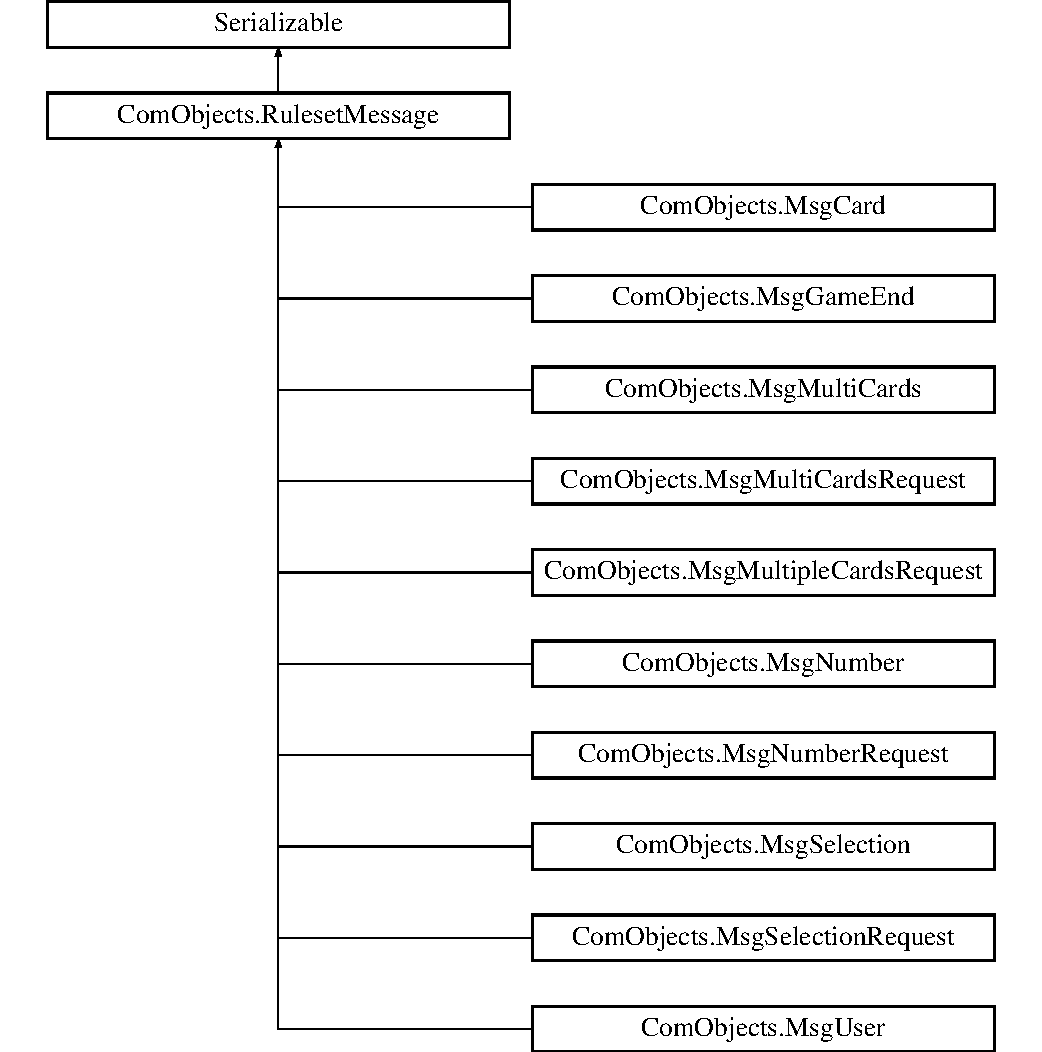
\includegraphics[height=12.000000cm]{a00075}
\end{center}
\end{figure}


\subsubsection{Ausführliche Beschreibung}
Sie enthält einen Nachrichtentyp und vererbt an alle Nachrichten für das Regelwerk. 
\hypertarget{a00076}{\subsection{Player Klassenreferenz}
\label{a00076}\index{Player@{Player}}
}


Abgeleitet von Runnable.

\subsubsection*{Öffentliche Methoden}
\begin{DoxyCompactItemize}
\item 
\hyperlink{a00076_a48d23656e2ce110dac280093f6d54190}{Player} (\hyperlink{a00077}{Server} lobby\-Server, Object\-Output\-Stream output, Object\-Input\-Stream input)
\item 
void \hyperlink{a00076_a13a43e6d814de94978c515cb084873b1}{run} ()
\item 
void \hyperlink{a00076_a13fa386dcc73d9e119b8af36f0cc9964}{send} (Com\-Object com)
\item 
void \hyperlink{a00076_a7656e712d839ef3c5013e7b909438111}{change\-Server} (\hyperlink{a00077}{Server} new\-Server)
\item 
String \hyperlink{a00076_a78ee178b6a73658d65ca60da4d1e6683}{get\-Name} ()
\item 
void \hyperlink{a00076_a772a23457853aff71a5c9a62c1b188a7}{set\-Name} (String new\-Name)
\end{DoxyCompactItemize}
\subsubsection*{Private Attribute}
\begin{DoxyCompactItemize}
\item 
\hypertarget{a00076_a9a2326f35466e54c36c070829245c557}{String \hyperlink{a00076_a9a2326f35466e54c36c070829245c557}{name}}\label{a00076_a9a2326f35466e54c36c070829245c557}

\item 
\hypertarget{a00076_afd1a82c786509e03b540bae82af2c137}{\hyperlink{a00077}{Server} \hyperlink{a00076_afd1a82c786509e03b540bae82af2c137}{server}}\label{a00076_afd1a82c786509e03b540bae82af2c137}

\item 
\hypertarget{a00076_a4a89fb49301c3bf13583a1ebbd622574}{Object\-Output\-Stream \hyperlink{a00076_a4a89fb49301c3bf13583a1ebbd622574}{com\-Out}}\label{a00076_a4a89fb49301c3bf13583a1ebbd622574}

\item 
\hypertarget{a00076_a9d3bfecfa3390ac5f668339005f961d6}{Object\-Input\-Stream \hyperlink{a00076_a9d3bfecfa3390ac5f668339005f961d6}{com\-In}}\label{a00076_a9d3bfecfa3390ac5f668339005f961d6}

\end{DoxyCompactItemize}


\subsubsection{Ausführliche Beschreibung}
Die Player-\/\-Klasse wird zum Versenden von Java Serializable Objects, sowie zum Annehmen solcher verwendet. Sie verwaltet fuer die Dauer einer Serververbindung die Verbindung zu einem Client. 

\subsubsection{Beschreibung der Konstruktoren und Destruktoren}
\hypertarget{a00076_a48d23656e2ce110dac280093f6d54190}{\index{Server\-::\-Player@{Server\-::\-Player}!Player@{Player}}
\index{Player@{Player}!Server::Player@{Server\-::\-Player}}
\paragraph[{Player}]{\setlength{\rightskip}{0pt plus 5cm}{\bf Player} (
\begin{DoxyParamCaption}
\item[{{\bf Server}}]{lobby\-Server, }
\item[{Object\-Output\-Stream}]{output, }
\item[{Object\-Input\-Stream}]{input}
\end{DoxyParamCaption}
)}}\label{a00076_a48d23656e2ce110dac280093f6d54190}


Konstruktor des Players, in ihm werden die Attribute server, com\-Out und com\-In mit vom Client\-Listerer\-Thread uebergebenen Werten Instanziiert. 


\begin{DoxyParams}{Parameter}
{\em lobby\-Server} & ist der \hyperlink{a00074}{Lobby\-Server}, der zu Beginn den \hyperlink{a00076}{Player} verwaltet. \\
\hline
{\em output} & ist der Object\-Output\-Stream an den entsprechenden Client \\
\hline
{\em input} & ist der Object\-Input\-Stream vom entsprechenden Client \\
\hline
\end{DoxyParams}


Benutzt Player.\-com\-In, Player.\-com\-Out und Player.\-server.



\subsubsection{Dokumentation der Elementfunktionen}
\hypertarget{a00076_a13a43e6d814de94978c515cb084873b1}{\index{Server\-::\-Player@{Server\-::\-Player}!run@{run}}
\index{run@{run}!Server::Player@{Server\-::\-Player}}
\paragraph[{run}]{\setlength{\rightskip}{0pt plus 5cm}void run (
\begin{DoxyParamCaption}
{}
\end{DoxyParamCaption}
)}}\label{a00076_a13a43e6d814de94978c515cb084873b1}


Die run-\/\-Methode des Thread nimmt eingehende Nachrichten des Client entgegen und uebergibt diese an den \hyperlink{a00077}{Server} durch Aufruf der Methode resolve\-Message() Faengt eine Class\-Not\-Found\-Exception ab, falls die Klasse nicht gefunden werden kann und gibt einen Fehler aus. 

Faengt eine I\-O\-Exception ab und ruft im jeweiligen \hyperlink{a00077}{Server}, dem er zugeteilt ist die handle\-I\-O\-Exception Methode auf. 

Benutzt Player.\-com\-In und Player.\-server.

\hypertarget{a00076_a13fa386dcc73d9e119b8af36f0cc9964}{\index{Server\-::\-Player@{Server\-::\-Player}!send@{send}}
\index{send@{send}!Server::Player@{Server\-::\-Player}}
\paragraph[{send}]{\setlength{\rightskip}{0pt plus 5cm}void send (
\begin{DoxyParamCaption}
\item[{Com\-Object}]{com}
\end{DoxyParamCaption}
)}}\label{a00076_a13fa386dcc73d9e119b8af36f0cc9964}


Diese Methode schickt ein Com\-Objekt an den Client. 

Sie faengt eine I\-O\-Exception ab und ruft im jeweiligen \hyperlink{a00077}{Server}, dem er zugeteilt ist die handle\-I\-O\-Exception Methode auf. 
\begin{DoxyParams}{Parameter}
{\em com} & ist das Com\-Object das verschickt wird \\
\hline
\end{DoxyParams}
\hypertarget{a00076_a7656e712d839ef3c5013e7b909438111}{\index{Server\-::\-Player@{Server\-::\-Player}!change\-Server@{change\-Server}}
\index{change\-Server@{change\-Server}!Server::Player@{Server\-::\-Player}}
\paragraph[{change\-Server}]{\setlength{\rightskip}{0pt plus 5cm}void change\-Server (
\begin{DoxyParamCaption}
\item[{{\bf Server}}]{new\-Server}
\end{DoxyParamCaption}
)}}\label{a00076_a7656e712d839ef3c5013e7b909438111}


Diese Methode wechselt beim \hyperlink{a00076}{Player} den \hyperlink{a00077}{Server} an den er com\-Objects weiterleiten soll. 

Dabei wird er aus dem player\-Set des alten Servers entfernt und in das player\-Set des neuen Players eingefuegt. Danach wird vom neuen \hyperlink{a00077}{Server} ein Com\-Update\-Playerlist Objekt mit broadcast an alle Clients, die vom \hyperlink{a00077}{Server} verwaltet werden, verschickt. 
\begin{DoxyParams}{Parameter}
{\em new\-Server} & ist der neue \hyperlink{a00077}{Server} \\
\hline
\end{DoxyParams}


Benutzt Player.\-get\-Name() und Player.\-server.

\hypertarget{a00076_a78ee178b6a73658d65ca60da4d1e6683}{\index{Server\-::\-Player@{Server\-::\-Player}!get\-Name@{get\-Name}}
\index{get\-Name@{get\-Name}!Server::Player@{Server\-::\-Player}}
\paragraph[{get\-Name}]{\setlength{\rightskip}{0pt plus 5cm}String get\-Name (
\begin{DoxyParamCaption}
{}
\end{DoxyParamCaption}
)}}\label{a00076_a78ee178b6a73658d65ca60da4d1e6683}


Getter-\/\-Methode fuer den Benutzernamen. 

\begin{DoxyReturn}{Rückgabe}
gibt den Benutzernamen des Spielers zurueck 
\end{DoxyReturn}


Benutzt Player.\-name.



Wird benutzt von Player.\-change\-Server().

\hypertarget{a00076_a772a23457853aff71a5c9a62c1b188a7}{\index{Server\-::\-Player@{Server\-::\-Player}!set\-Name@{set\-Name}}
\index{set\-Name@{set\-Name}!Server::Player@{Server\-::\-Player}}
\paragraph[{set\-Name}]{\setlength{\rightskip}{0pt plus 5cm}void set\-Name (
\begin{DoxyParamCaption}
\item[{String}]{new\-Name}
\end{DoxyParamCaption}
)}}\label{a00076_a772a23457853aff71a5c9a62c1b188a7}


Setter-\/\-Methode fuer den Benutzernamen. 


\begin{DoxyParams}{Parameter}
{\em new\-Name} & ist der neue Name \\
\hline
\end{DoxyParams}


Benutzt Player.\-name.


\hypertarget{a00077}{\subsection{Client.\-View.\-Score\-Window Klassenreferenz}
\label{a00077}\index{Client.\-View.\-Score\-Window@{Client.\-View.\-Score\-Window}}
}
Klassendiagramm für Client.\-View.\-Score\-Window\-:\begin{figure}[H]
\begin{center}
\leavevmode
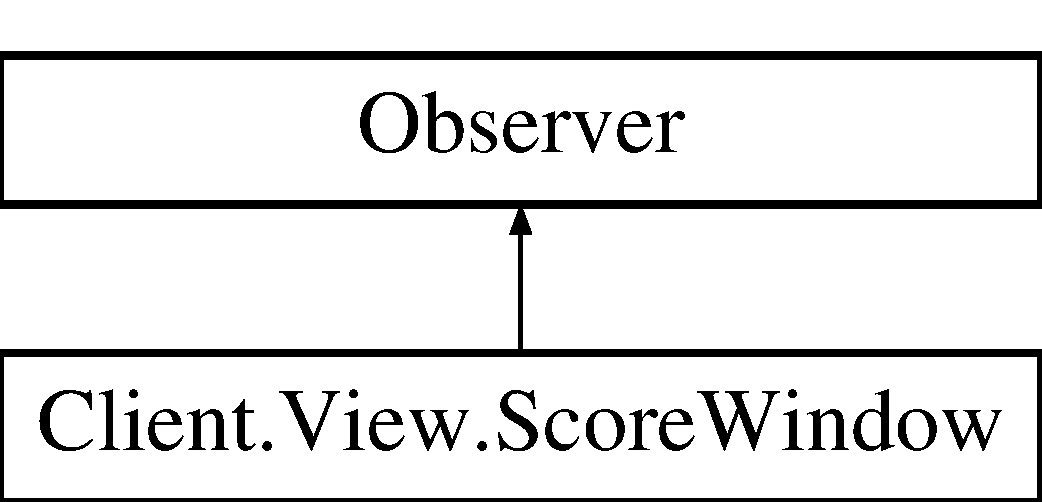
\includegraphics[height=2.000000cm]{a00077}
\end{center}
\end{figure}
\subsubsection*{Öffentliche Methoden}
\begin{DoxyCompactItemize}
\item 
void \hyperlink{a00077_a5b5198d8d5970e4d15737c809f44b65d}{update} (Observable o, Object arg)
\end{DoxyCompactItemize}


\subsubsection{Ausführliche Beschreibung}
\begin{DoxyAuthor}{Autor}
m4nkey 
\end{DoxyAuthor}


\subsubsection{Dokumentation der Elementfunktionen}
\hypertarget{a00077_a5b5198d8d5970e4d15737c809f44b65d}{\index{Client\-::\-View\-::\-Score\-Window@{Client\-::\-View\-::\-Score\-Window}!update@{update}}
\index{update@{update}!Client::View::ScoreWindow@{Client\-::\-View\-::\-Score\-Window}}
\paragraph[{update}]{\setlength{\rightskip}{0pt plus 5cm}void Client.\-View.\-Score\-Window.\-update (
\begin{DoxyParamCaption}
\item[{Observable}]{o, }
\item[{Object}]{arg}
\end{DoxyParamCaption}
)}}\label{a00077_a5b5198d8d5970e4d15737c809f44b65d}


Wird durch notify() im \hyperlink{a00013}{Client\-Model} aufgerufen. 

Je nach dem in arg �bergebenen Befehl wird ein Update des Fensters ausgef�hrt oder eine Fehlermeldung angezeigt.


\begin{DoxyParams}{Parameter}
{\em o} & erwartet ein Objekt von der Klasse \hyperlink{a00013}{Client\-Model} \\
\hline
{\em arg} & erwartet\-: show\-Score \\
\hline
\end{DoxyParams}

\hypertarget{a00078}{\subsection{Server.\-Server Klassenreferenz}
\label{a00078}\index{Server.\-Server@{Server.\-Server}}
}
Klassendiagramm für Server.\-Server\-:\begin{figure}[H]
\begin{center}
\leavevmode
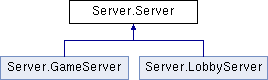
\includegraphics[height=2.000000cm]{a00078}
\end{center}
\end{figure}
\subsubsection*{Öffentliche Methoden}
\begin{DoxyCompactItemize}
\item 
void \hyperlink{a00078_a248b5c6e75df5be16fb281ac194c7e20}{receive\-Message} (\hyperlink{a00073}{Player} player, \hyperlink{a00029}{Com\-Object} com)
\item 
synchronized void \hyperlink{a00078_a752adb06d6c1e59797bdb2dde5c9058b}{send\-To\-Player} (String name, \hyperlink{a00029}{Com\-Object} com)
\item 
synchronized void \hyperlink{a00078_a84083f41e9cbad43bca45072e64877ee}{add\-Player} (\hyperlink{a00073}{Player} player)
\item 
synchronized void \hyperlink{a00078_adbd5ca08d0f660116673717e38db0343}{remove\-Player} (\hyperlink{a00073}{Player} player)
\item 
synchronized void \hyperlink{a00078_a32695e6a4c0f39af5c7e867384cc3ba7}{broadcast} (\hyperlink{a00029}{Com\-Object} com)
\end{DoxyCompactItemize}


\subsubsection{Ausführliche Beschreibung}
Es stellt Methoden zur Nachrichtenversendung und -\/verarbeitung bereit, sowie zur Verwaltung von Playern \begin{DoxyAuthor}{Autor}
Viktoria 
\end{DoxyAuthor}


\subsubsection{Dokumentation der Elementfunktionen}
\hypertarget{a00078_a84083f41e9cbad43bca45072e64877ee}{\index{Server\-::\-Server@{Server\-::\-Server}!add\-Player@{add\-Player}}
\index{add\-Player@{add\-Player}!Server::Server@{Server\-::\-Server}}
\paragraph[{add\-Player}]{\setlength{\rightskip}{0pt plus 5cm}synchronized void Server.\-Server.\-add\-Player (
\begin{DoxyParamCaption}
\item[{{\bf Player}}]{player}
\end{DoxyParamCaption}
)}}\label{a00078_a84083f41e9cbad43bca45072e64877ee}


Diese Methode f�gt einen \hyperlink{a00073}{Player} dem Set an Playern hinzu, welche der \hyperlink{a00078}{Server} verwaltet. 


\begin{DoxyParams}{Parameter}
{\em player} & ist der \hyperlink{a00073}{Player}, der hinzugefo�gt wird \\
\hline
\end{DoxyParams}
\hypertarget{a00078_a32695e6a4c0f39af5c7e867384cc3ba7}{\index{Server\-::\-Server@{Server\-::\-Server}!broadcast@{broadcast}}
\index{broadcast@{broadcast}!Server::Server@{Server\-::\-Server}}
\paragraph[{broadcast}]{\setlength{\rightskip}{0pt plus 5cm}synchronized void Server.\-Server.\-broadcast (
\begin{DoxyParamCaption}
\item[{{\bf Com\-Object}}]{com}
\end{DoxyParamCaption}
)}}\label{a00078_a32695e6a4c0f39af5c7e867384cc3ba7}


Diese Methode wird genutzt, um ein Com\-Object an alle Clients, die vom \hyperlink{a00078}{Server} verwaltet werden, zu schicken. 


\begin{DoxyParams}{Parameter}
{\em com} & ist das Com\-Object, dass verschickt werden soll \\
\hline
\end{DoxyParams}
\hypertarget{a00078_a248b5c6e75df5be16fb281ac194c7e20}{\index{Server\-::\-Server@{Server\-::\-Server}!receive\-Message@{receive\-Message}}
\index{receive\-Message@{receive\-Message}!Server::Server@{Server\-::\-Server}}
\paragraph[{receive\-Message}]{\setlength{\rightskip}{0pt plus 5cm}void Server.\-Server.\-receive\-Message (
\begin{DoxyParamCaption}
\item[{{\bf Player}}]{player, }
\item[{{\bf Com\-Object}}]{com}
\end{DoxyParamCaption}
)}}\label{a00078_a248b5c6e75df5be16fb281ac194c7e20}


Diese Methode dient zur Verarbeitung von eingehenden Com\-Objects. 


\begin{DoxyParams}{Parameter}
{\em player} & ist der \hyperlink{a00073}{Player} von dem die Nachricht kommt \\
\hline
{\em com} & ist das Com\-Objekt vom Client verschickt wurde \\
\hline
\end{DoxyParams}
\hypertarget{a00078_adbd5ca08d0f660116673717e38db0343}{\index{Server\-::\-Server@{Server\-::\-Server}!remove\-Player@{remove\-Player}}
\index{remove\-Player@{remove\-Player}!Server::Server@{Server\-::\-Server}}
\paragraph[{remove\-Player}]{\setlength{\rightskip}{0pt plus 5cm}synchronized void Server.\-Server.\-remove\-Player (
\begin{DoxyParamCaption}
\item[{{\bf Player}}]{player}
\end{DoxyParamCaption}
)}}\label{a00078_adbd5ca08d0f660116673717e38db0343}


Diese Methode entfernt einen \hyperlink{a00073}{Player} aus dem Set an Playern, welche der \hyperlink{a00078}{Server} verwaltet. 


\begin{DoxyParams}{Parameter}
{\em player} & ist der \hyperlink{a00073}{Player}, der entfernt wird \\
\hline
\end{DoxyParams}
\hypertarget{a00078_a752adb06d6c1e59797bdb2dde5c9058b}{\index{Server\-::\-Server@{Server\-::\-Server}!send\-To\-Player@{send\-To\-Player}}
\index{send\-To\-Player@{send\-To\-Player}!Server::Server@{Server\-::\-Server}}
\paragraph[{send\-To\-Player}]{\setlength{\rightskip}{0pt plus 5cm}synchronized void Server.\-Server.\-send\-To\-Player (
\begin{DoxyParamCaption}
\item[{String}]{name, }
\item[{{\bf Com\-Object}}]{com}
\end{DoxyParamCaption}
)}}\label{a00078_a752adb06d6c1e59797bdb2dde5c9058b}


Diese Methode wird genutzt, um ein Com\-Object an einen einzigen Client zu verschicken. 

Der \hyperlink{a00073}{Player} der die Nachricht verschicken soll wird Anhand des �bergebenen Benutzernamens identifiziert. 
\begin{DoxyParams}{Parameter}
{\em name} & ist der Name des Clients, an den der \hyperlink{a00073}{Player} die Nachricht verschicken soll \\
\hline
{\em c} & ist das Com\-Object, dass verschickt werden soll \\
\hline
\end{DoxyParams}

%--- End generated contents ---
\section{JUnit-Tests}
JUnit-Tests werden für die folgenden Klassen geschrieben: ClientModel, LobbyServer,
GameServer, ClientHearts, ClientWizard, ServerHearts und ServerWizard. Für die folgenden Fälle wurden bereits Tests implementiert.

\subsection{isValidWizardMove}
\begin{lstlisting}
package Ruleset;


import static org.junit.Assert.assertFalse;
import static org.junit.Assert.assertTrue;

import org.junit.After;
import org.junit.Before;
import org.junit.Test;

import test.TestGameServer;
import test.TestLobbyServer;
import test.TestPlayer;

import Server.GameServer;
import Server.LobbyServer;
import Server.Player;

public class TestisValidMoveWizard {
	
	ServerRuleset ruleset;
	
	GameServer gameServer;
	
	LobbyServer lobbyServer;
	
	Player player;
	String player1;
	String player2;
	String player3;
	PlayerState playerState1;
	PlayerState playerState2;
	PlayerState playerState3;
	
	@Before
	public void setUp() throws Exception {
		player1 = "Tick";
		player2 = "Trick";
		player3 = "Track";
		lobbyServer = new TestLobbyServer();
		player = new TestPlayer(lobbyServer,null,null);
		gameServer = new TestGameServer(lobbyServer,player,"Mein Spiel",RulesetType.Wizard, 
				"",false);
		ruleset = new ServerWizard(gameServer);
		
		ruleset.addPlayerToGame(player1);
		ruleset.addPlayerToGame(player2);
		ruleset.addPlayerToGame(player3);
		
		playerState1 = ruleset.getPlayerState(player1);
		playerState2 = ruleset.getPlayerState(player2);
		playerState3 = ruleset.getPlayerState(player3);
		
		ruleset.setFirstPlayer(ruleset.getPlayerState(player1));
		ruleset.setTrumpCard(WizardCard.VierRot);
		
		ruleset.giveACard(playerState1, WizardCard.DreiGruen);
		ruleset.giveACard(playerState1, WizardCard.ZaubererRot);
		ruleset.givaACard(playerState1, WizardCard.ZweiBlau);
		
		ruleset.giveACard(playerState2, WizardCard.ZweiGruen);
		ruleset.giveACard(playerState2, WizardCard.DreiRot);
		ruleset.givaACard(playerState2, WizardCard.ZweiGelb);
		
		ruleset.giveACard(playerState3, WizardCard.NarrBlau);
		ruleset.giveACard(playerState3, WizardCard.EinsGruen);
		ruleset.giveACard(playerState3, WizardCard.ZweiRot);
	}
	
	@Test
	public void testSorcerer() {
		ruleset.playCard(WizardCard.ZaubererRot);
		ruleset.setCurrentPlayer(playerState2);
		
		boolean isValidMove = ruleset.isValidMove(WizardCard.DreiRot);
		
		assertTrue(isValidMove);
	}
	
	@Test
	public void testRed3OnGreen3() {
		ruleset.playCard(WizardCard.DreiGruen);
		ruleset.setCurrentPlayer(playerState2);
		boolean isValidMove = ruleset.isValidMove(WizardCard.DreiRot);
		
		assertFalse(isValidMove);
	}
	
	@Test
	public void testGreen2OnGreen3() {
		ruleset.playCard(WizardCard.DreiGruen);
		ruleset.setCurrentPlayer(playerState2);
		
		boolean isValidMove = ruleset.isValidMove(WizardCard.ZweiGruen);
		
		assertTrue(isValidMove);
	}
	
	@Test
	public void testFoolBlueOnGreen2OnGreen3() {
		ruleset.playCard(WizardCard.DreiGruen);
		ruleset.setCurrentPlayer(playerState2);
		
		ruleset.playCard(WizardCard.ZweiGruen);
		ruleset.setCurrentPlayer(playerState3);
		
		boolean isValidMove = ruleset.isValidMove(WizardCard.NarrBlau);
		
		assertTrue(isValidMove);
	}

}
\end{lstlisting}

\subsection{isValidHeartsMove}
\begin{lstlisting}
package Ruleset;


import static org.junit.Assert.*;
import static org.junit.Assert.assertEquals;

import org.junit.Before;
import org.junit.Test;

import test.TestGameServer;
import test.TestLobbyServer;
import test.TestPlayer;

import Server.GameServer;
import Server.LobbyServer;
import Server.Player;

public class TestisValidMoveHearts {
	ServerRuleset ruleset;
	
	GameServer gameServer;
	
	LobbyServer lobbyServer;
	
	Player player;
	String player1;
	String player2;
	String player3;
	String player4;
	
	PlayerState playerState1;
	PlayerState playerState2;
	PlayerState playerState3;
	PlayerState playerState4;
	
	@Before
	public void setUp() throws Exception {
		player1 = "Tick";
		player2 = "Trick";
		player3 = "Track";
		player3 = "Duck";
		lobbyServer = new TestLobbyServer();
		player = new TestPlayer(lobbyServer,null,null);
		gameServer = new TestGameServer(lobbyServer,player,"Mein Spiel",
				RulesetType.Hearts, "",false);
		ruleset = new ServerHearts(gameServer);
		
		ruleset.addPlayerToGame(player1);
        ruleset.addPlayerToGame(player2);
        ruleset.addPlayerToGame(player3);
        ruleset.addPlayerToGame(player4);
        
        playerState1 = ruleset.getPlayerState(player1);
        playerState2 = ruleset.getPlayerState(player2);
        playerState3 = ruleset.getPlayerState(player3);

        ruleset.setFirstPlayer(playerState1);
	}
	
	@Test
	public void testIsValidMove() {
		 ruleset.giveACard(playerState1, HeartsCard.Herz2);
	     ruleset.giveACard(playerState1, HeartsCard.Kreuz9);
	     ruleset.giveACard(playerState2, HeartsCard.Caro3);
	     ruleset.giveACard(playerState2, HeartsCard.Caro6);
	     ruleset.giveACard(playerState3, HeartsCard.Pik4);
	     ruleset.giveACard(playerState3, HeartsCard.Pik5);
         ruleset.giveACard(playerState4, HeartsCard.Pik1);
	     ruleset.giveACard(playerState4, HeartsCard.Herz7);
	     
	     boolean isValidMove = ruleset.isValidMove(HeartsCard.Herz2);

	     assertFalse(isValidMove);

	     boolean isValidMove2 = ruleset.isValidMove(HeartsCard.Caro3);
	     
	     assertTrue(isValidMove2);
	}
	
	@Test
	public void testIsValidMoveOnlyHearts() {
		 ruleset.giveACard(playerState1, HeartsCard.Herz2);
	     ruleset.giveACard(playerState1, HeartsCard.Herz5);
	     ruleset.giveACard(playerState2, HeartsCard.Caro3);
	     ruleset.giveACard(playerState2, HeartsCard.Caro6);
	     ruleset.giveACard(playerState3, HeartsCard.Pik4);
	     ruleset.giveACard(playerState3, HeartsCard.Pik5);
         ruleset.giveACard(playerState4, HeartsCard.Pik1);
	     ruleset.giveACard(playerState4, HeartsCard.Herz7);
	     
	     boolean isValidMove = ruleset.isValidMove(HeartsCard.Herz2);

	     assertTrue(isValidMove);

	     boolean isValidMove2 = ruleset.isValidMove(HeartsCard.Herz5);
	     
	     assertTrue(isValidMove2);
	}

}
\end{lstlisting}

\subsection{getWinner}
\begin{lstlisting}
package Ruleset;

import static org.junit.Assert.*;

import java.util.List;

import org.junit.After;
import org.junit.Before;
import org.junit.Test;
import testKlassen.TestPlayer;
import ComObjects.ComObject;
import ComObjects.ComRuleset;
import ComObjects.MsgGameEnd;
import Server.GameServer;
import Server.LobbyServer;
import Server.Player;

public class TestHeartsWinner {

LobbyServer lobbyServer;
	
	GameServer gameServer;
	
	ServerRuleset heartsServerRuleset;
	
	TestPlayer blue;
	
	TestPlayer white;
	
	TestPlayer orange;
	
	TestPlayer brown;
	
	List<ComObject> inputList;
	
	ComRuleset comObject;
	
	MsgGameEnd endMsg;
	
	String winner;
	
	@Before
	public void setUp() {
		lobbyServer = new LobbyServer();
		blue = new TestPlayer(lobbyServer, null, null);
		white = new TestPlayer(lobbyServer, null, null);
		orange = new TestPlayer(lobbyServer, null, null);
		brown = new TestPlayer(lobbyServer, null, null);
	}
	
	@After
	public void tearDown() {	
		blue = null;
		white = null;
		orange = null;
		brown = null;
		lobbyServer = null;
		gameServer = null;
		inputList = null;
		comObject = null;
		endMsg = null;
		winner = null;
	}
	
	@Test
	public void testGetWinner() {
		
		gameServer = new GameServer(lobbyServer, blue, "Test Game", RulesetType.Wizard, "", false);
		gameServer.addPlayer(white);
		gameServer.addPlayer(orange);
		gameServer.addPlayer(brown);
		
		heartsServerRuleset = new ServerWizard(gameServer);
		heartsServerRuleset.addPlayerToGame("Mr. Blue");
		heartsServerRuleset.addPlayerToGame("Mr. White");
		heartsServerRuleset.addPlayerToGame("Mr. Orange");
		heartsServerRuleset.addPlayerToGame("Mr. Brown");
		heartsServerRuleset.setPoints(heartsServerRuleset.getPlayerState("Mr. Blue"),80);
		heartsServerRuleset.setPoints(heartsServerRuleset.getPlayerState("Mr. White"),20);
		heartsServerRuleset.setPoints(heartsServerRuleset.getPlayerState("Mr. Orange"),60);
		heartsServerRuleset.setPoints(heartsServerRuleset.getPlayerState("Mr. Brown"),110);
		heartsServerRuleset.setGamePhase(GamePhase.Ending);
		heartsServerRuleset.calculateRoundOutcome();
		
		assertTrue(heartsServerRuleset.getWinner().equals("Mr. Brown"));
		
		inputList = blue.getServerInput();
		comObject = (ComRuleset) inputList.get(1);
		endMsg = (MsgGameEnd) comObject.getRulesetMessage();
		winner = endMsg.getWinner();
		assertEquals("Nachricht an Blue", "Mr. Brown", winner);

		inputList = white.getServerInput();
		comObject = (ComRuleset) inputList.get(1);
		endMsg = (MsgGameEnd) comObject.getRulesetMessage();
		winner = endMsg.getWinner();
		assertEquals("Nachricht an White", "Mr. Brown", winner);

		inputList = orange.getServerInput();
		comObject = (ComRuleset) inputList.get(1);
		endMsg = (MsgGameEnd) comObject.getRulesetMessage();
		winner = endMsg.getWinner();
		assertEquals("Nachricht an Orange", "Mr. Brown", winner);
	
		inputList = brown.getServerInput();
		comObject = (ComRuleset) inputList.get(1);
		endMsg = (MsgGameEnd) comObject.getRulesetMessage();
		winner = endMsg.getWinner();
		assertEquals("Nachricht an Brown", "Mr. Brown", winner);
	}
}
\end{lstlisting}

\begin{lstlisting}
package Ruleset;

import static org.junit.Assert.*;

import java.util.List;

import org.junit.After;
import org.junit.Before;
import org.junit.Test;
import testKlassen.TestPlayer;
import ComObjects.ComChatMessage;
import ComObjects.ComObject;
import ComObjects.ComRuleset;
import ComObjects.MsgGameEnd;
import Server.GameServer;
import Server.LobbyServer;

/**
 * Testet ob der richtige Sieger ermittelt wird und ob jedem Mitspieler
 * der richtige Sieger mitgeteilt wird
 */
public class TestWizardWinner {

	LobbyServer lobbyServer;
	
	GameServer gameServer;
	
	ServerRuleset wizardServerRuleset;
	
	TestPlayer blue;
	
	TestPlayer white;
	
	TestPlayer orange;
	
	TestPlayer brown;
	
	List<ComObject> inputList;
	
	ComRuleset comObject;
	
	MsgGameEnd endMsg;
	
	String winner;
	
	@Before
	public void setUp() {
		lobbyServer = new LobbyServer();
		blue = new TestPlayer(lobbyServer, null, null);
		white = new TestPlayer(lobbyServer, null, null);
		orange = new TestPlayer(lobbyServer, null, null);
		brown = new TestPlayer(lobbyServer, null, null);
	}
	
	@After
	public void tearDown() {	
		blue = null;
		white = null;
		orange = null;
		brown = null;
		lobbyServer = null;
		gameServer = null;
		inputList = null;
		inputList = null;
		comObject = null;
		endMsg = null;
		winner = null;
	}
	
	@Test
	public void testGetWinner() {
		
		gameServer = new GameServer(lobbyServer, blue, "Test Game", RulesetType.Wizard, "", false);
		gameServer.addPlayer(white);
		gameServer.addPlayer(orange);
		gameServer.addPlayer(brown);
		
		wizardServerRuleset = new ServerWizard(gameServer);
		wizardServerRuleset.addPlayerToGame("Mr. Blue");
		wizardServerRuleset.addPlayerToGame("Mr. White");
		wizardServerRuleset.addPlayerToGame("Mr. Orange");
		wizardServerRuleset.addPlayerToGame("Mr. Brown");
		wizardServerRuleset.setPoints(wizardServerRuleset.getPlayerState("Mr. Blue"),80);
		wizardServerRuleset.setPoints(wizardServerRuleset.getPlayerState("Mr. White"),200);
		wizardServerRuleset.setPoints(wizardServerRuleset.getPlayerState("Mr. Orange"),130);
		wizardServerRuleset.setPoints(wizardServerRuleset.getPlayerState("Mr. Brown"),240);
		wizardServerRuleset.setGamePhase(GamePhase.Ending);
		wizardServerRuleset.calculateRoundOutcome();
		
		assertTrue(wizardServerRuleset.getWinner().equals("Mr. Brown"));
		
		inputList = blue.getServerInput();
		comObject = (ComRuleset) inputList.get(1);
		endMsg = (MsgGameEnd) comObject.getRulesetMessage();
		winner = endMsg.getWinner();
		assertEquals("Nachricht an Blue", "Mr. Brown", winner);

		inputList = white.getServerInput();
		comObject = (ComRuleset) inputList.get(1);
		endMsg = (MsgGameEnd) comObject.getRulesetMessage();
		winner = endMsg.getWinner();
		assertEquals("Nachricht an White", "Mr. Brown", winner);

		inputList = orange.getServerInput();
		comObject = (ComRuleset) inputList.get(1);
		endMsg = (MsgGameEnd) comObject.getRulesetMessage();
		winner = endMsg.getWinner();
		assertEquals("Nachricht an Orange", "Mr. Brown", winner);
	
		inputList = brown.getServerInput();
		comObject = (ComRuleset) inputList.get(1);
		endMsg = (MsgGameEnd) comObject.getRulesetMessage();
		winner = endMsg.getWinner();
		assertEquals("Nachricht an Brown", "Mr. Brown", winner);
	}
}

\end{lstlisting}

\subsection{QuitPlayer}
\begin{lstlisting}
ackage Server;


import static org.junit.Assert.*;

import java.io.BufferedInputStream;
import java.io.IOException;
import java.io.ObjectInputStream;
import java.io.ObjectOutputStream;
import java.util.ArrayList;
import java.util.List;

import org.junit.After;
import org.junit.Before;
import org.junit.Test;

import test.TestGameServer;
import test.TestLobbyServer;
import test.TestPlayer;

import ComObjects.*;
import ComObjects.ComWarning;
import Ruleset.RulesetType;

public class QuitGameTest {

	TestLobbyServer lobby;
	
	TestPlayer player1; 
	
	TestPlayer player2; 
	TestPlayer player3;
	TestPlayer player4;
	
	TestGameServer game;
	
	ComClientQuit quit;
	
	@Before
	public void setUp() throws Exception {
		lobby = new TestLobbyServer();
		
		player1 = new TestPlayer(lobby, null, null);
		player1.setName("MrBlue");
		lobby.addPlayer(player1);
		
		player2 = new TestPlayer(lobby, null, null);
		player2.setName("MrWhite");
		player3 = new TestPlayer(lobby, null, null);
		player3.setName("MrPink");
		player4 = new TestPlayer(lobby, null, null);
		player4.setName("MrRed");
		
		game = new TestGameServer(lobby, player1, "MrBluesGame", RulesetType.Hearts, null, false);
		
		game.addPlayer(player2);
		game.addPlayer(player3);
		game.addPlayer(player4);
		
		quit = new ComClientQuit();
	}

	@After
	public void tearDown() throws Exception {
		lobby = null;
		player1 = null;
		player2 = null;
		player3 = null;
		player4 = null;
		game = null;
	}
	
	@Test
	public void testPlayerQuitGame() throws IOException{ 
		
		player1.changeServer(game);
		assertTrue(game.initLobby().getPlayerList().contains(player1.getName()));
		
		ComInitLobby initLobby = lobby.initLobby();
		ComWarning warning = new ComWarning("Ein Spieler hat das Spiel verlassen");
		
		player1.injectComObject(quit);

		assertFalse(lobby.initLobby().getGameList().contains(game));
		assertTrue(lobby.initLobby().getPlayerList().contains(player1.getName()));
		assertTrue(lobby.initLobby().getPlayerList().contains(player1.getName()));
		assertTrue(lobby.initLobby().getPlayerList().contains(player1.getName()));
		assertTrue(lobby.initLobby().getPlayerList().contains(player1.getName()));
		
		assertTrue(player1.getServerInput().get(0).getClass() == initLobby.getClass());
		assertTrue(player1.getServerInput().get(1).getClass() == warning.getClass());
		assertTrue(player2.getServerInput().get(0).getClass() == initLobby.getClass());
		assertTrue(player2.getServerInput().get(1).getClass() == warning.getClass());
		assertTrue(player3.getServerInput().get(0).getClass() == initLobby.getClass());
		assertTrue(player3.getServerInput().get(1).getClass() == warning.getClass());
		assertTrue(player4.getServerInput().get(0).getClass() == initLobby.getClass());
		assertTrue(player4.getServerInput().get(1).getClass() == warning.getClass());
	}
}
\end{lstlisting}

\subsection{Chat}

\begin{lstlisting}
package chat;

import static org.junit.Assert.*;

import org.junit.Test;
import org.junit.After;
import org.junit.Before;

import testKlassen.TestMessageListenerThread;
import testKlassen.TestObserver;
import Client.MessageListenerThread;
import Client.ClientModel;
import ComObjects.ComChatMessage;

public class ClientModelChatTest {

	ComChatMessage testMessage;
	
	ClientModel testModel;
	
	TestObserver testObserver;
	
	TestMessageListenerThread testNetIO;
	
	String testText;
	
	@Before  
    public void setUp() {
		testNetIO = new TestMessageListenerThread();
		testObserver = new TestObserver();
		testMessage = new ComChatMessage("Hello Test!");
		testModel = new ClientModel((MessageListenerThread) testNetIO);
		testNetIO.setModel(testModel);
		testModel.addObserver(testObserver);
    }  
  
    @After  
    public void tearDown() { 
    	testNetIO = null;
    	testMessage = null;
    	testModel = null;
    	testObserver = null;
    }  
	
	@Test
	public void testSendChatMessage() {
		String inputText = "Hello Test!";
		testModel.sendChatMessage(inputText);
		testText = ((ComChatMessage) testNetIO.getModelInput().get(0)).getChatMessage();
		assertEquals("Vergleich der gesendeten Chatnachrichten", testText, inputText);
	}
	
	@Test
	public void testReceiveChatMessage() {
		testNetIO.injectComObject(testMessage);
		assertTrue("Vergleich der empfangenen Chatnachrichten", 
				testObserver.getChatMessage().equals(testMessage.getChatMessage()));
	}
}
\end{lstlisting}

\begin{lstlisting}
package chat;

import static org.junit.Assert.*;

import org.junit.After;
import org.junit.Before;
import org.junit.Test;

import testKlassen.TestPlayer;
import Server.LobbyServer;
import ComObjects.ComChatMessage;

public class LobbyServerChatTest {

	ComChatMessage testMessage;
	
	LobbyServer testServer;

	TestPlayer player1;
	
	TestPlayer player2;
	
	TestPlayer player3;
	
	String testText1;
	
	String testText2;
	
	String testText3;

	@Before
	public void setUp() {
		testMessage = new ComChatMessage("Hello Test!");
		testServer = new LobbyServer();
		player1 = new TestPlayer(testServer, null, null);
		player2 = new TestPlayer(testServer, null, null);
		player3 = new TestPlayer(testServer, null, null);
	}

	@After
	public void tearDown() {
		testMessage = null;
		testServer = null;
		player1 = null;
		player2 = null;
		player3 = null;
		testText1 = null;
		testText2 = null;
		testText3 = null;
	}

	@Test
	public void testReceiveMessagePlayerComChatMessage() {
		String messageToMatch = testMessage.getChatMessage();
		testServer.addPlayer(player1);
		testServer.addPlayer(player2);
		testServer.addPlayer(player3);
		player1.injectComObject(testMessage);
		testText1 = ((ComChatMessage) player1.getServerInput()).getChatMessage();
		testText2 = ((ComChatMessage) player2.getServerInput()).getChatMessage();
		testText3 = ((ComChatMessage) player3.getServerInput()).getChatMessage();
		assertEquals("Nachricht an Spieler 1", messageToMatch, testText1);
		assertEquals("Nachricht an Spieler 2", messageToMatch, testText2);
		assertEquals("Nachricht an Spieler 3", messageToMatch, testText3);
	}
}

\end{lstlisting}

\section{Implementierungsplan}
Es werden für jeden Milestone die einzelnen Arbeitspakete angegeben. Die angegebenen Klassen werden nicht sofort vollständig implmentiert, sondern mit den vom Arbeitspaket und Milestone verlangten Funktionen ausgestattet.\\

\subsection{Milestone 1}
Für den ersten Milestone werden folgende Funktionen angestrebt:\\
Der Nutzer kann sich im Login-Fenster anmelden und die Lobby betreten. Er kann ein Spiel erstellen und offenen Spielen beitreten. Das wird in der Lobby angezeigt, man gelangt jedoch noch nicht ins Wartefenster. Nebenläufig dazu wird die Datenschicht der Regelwerke implementiert.\\ 
\begin{itemize}
\item View(Login+Lobby) Dauer: 8 Std. \\
Klassen: Login, Lobby, Warning, ClientController
\item Client(Login) Dauer 8 Std. \\
Klassen: ClientMain, ClientModel, MessageListener Thread, ClientState, ViewNotification
\item Server(Login) Dauer 16 Std. \\
Klassen: Server, ServerMain, LobbyServer, Player, ClientListenerThread, ComObject, ComLoginRequest, ComClientQuit, ComServerAcknowledgement, ComWarning
\item Ruleset(Daten) Dauer 20 Std. \\
Klassen:  Card, Colour, HeartsCard, WizCard, OtherData, WizData, HeartsData, GameClientUpdate, GameState, PlayerState, RulesetType
\item Client(Lobby) Dauer 8 Std. \\
Klassen: ClientModel
\item Server(Lobby) Dauer 8 Std. \\
Klassen: LobbyServer, ComChatMessage, ComLobbyUpdateGamelist, ComJoinRequest, ComInitLobby, ComUpdatePlayerlist
\item View(Create+Join) Dauer 8 Std. \\
Klassen: Password, CreateGame, ClientController
\item Client(Create+Join) Dauer 8 Std. \\
Klassen: ClientModel
\item Server(Create+Join) Dauer 12 Std. \\
Klassen: LobbyServer, ComJoinRequest, ComCreateGameRequest
\end{itemize}

\subsection{Milestone 2}
Für den zweiten Milestone werden folgende Funktionen angestrebt:\\
Beim Beitreten oder Erstellen eines Spiels gelangt man ins Wartefenster. Der Spielleiter kannn hier Spieler entfernen. Diese gelangen zurück in die Lobby. Das Spiel kann noch nicht gestartet werden, aber das Regelwerk wird bereits serverseitig implementiert.\\
\begin{itemize}
\item Ruleset(Wizard-Server) Dauer 30 Std. \\
Klassen: ServerRuleset, ServerWizard, RulesetMessage, MsgCard, MsgCardRequest, MsgGameEnd, MsgNumber, Msg NumberRequest, MsgSelection, MsgSelectionRequest, MsgUser
\item View(GameLobby) Dauer 8 Std. \\
Klassen: GameLobby, ClientController
\item Client(GameLobby) Dauer 8 Std. \\
Klassen: ClientModel
\item Server(GameLobby) Dauer 10 Std. \\
KLassen: LobbyServer, GameServer, ComBeenKicked, ComClientLeave, ComInitGameLobby, ComKickPlayerRequest, ComStartGame
\item View(Game) Dauer 20 Std. \\
Klassen: Game, GamePanel, OtherPlayer, OwnHand, ViewCard, DrawDeck, DiscardPile, ScoreWindow, ClientController
\item Client(Game) Dauer 14 Std. \\
Klassen: ClientModel
\end{itemize}

\subsection{Milestone 3}
Für den dritten Milestone werden folgende Funktionen angestrebt:\\
Es kann schon eine vollständige Partie Wizard gespielt werden.\\
\begin{itemize}
\item Server(Game) Dauer 4 Std. \\
Klassen: GameServer, ComStartGame, ComRuleset, ComGameEnd
\item Ruleset(Wizard-Client) Dauer 12 Std. \\
Klassen: ClientWizard
\item View(WizardWindows) Dauer 4 Std. \\
Klassen: ChooseItem, InputNumber, ClientController
\item Client(Wizard) Dauer 6 Std. \\
Klassen: ClientModel
\item View(HeartsWindows) Dauer 2 Std. \\
Klassen: ChooseCards, ClientController
\item Client(Hearts) Dauer 4 Std. \\
Klassen: ClientModel
\item Ruleset(Hearts-Server) Dauer 16 Std. \\
Klassen: ServerHearts
\end{itemize}

\subsection{Finale Version}
Die finale Version enthält die volle Funktionalität des Programs.
Es können also sowohl Wizard als auch Hearts gespielt werden.\\
\begin{itemize}
\item Ruleset(Hearts-Client) Dauer 10Std. \\
Klassen: ClientHearts
\item ViewPolishing(evtl Tests) Dauer 10Std \\
Verbesserungen an der bisherigen Implementierung. Gegebenfalls Schreiben von zusätzlichen Tests
\item ClientPolishing(evtl Tests) Dauer 10Std \\
Verbesserungen an der bisherigen Implementierung. Gegebenfalls Schreiben von zusätzlichen Tests
\item ServerPolishing(evtl Tests) Dauer 10Std \\
Verbesserungen an der bisherigen Implementierung. Gegebenfalls Schreiben von zusätzlichen Tests
\item RulesetPolishing(evtl Tests) Dauer 10Std \\
Verbesserungen an der bisherigen Implementierung. Gegebenfalls Schreiben von zusätzlichen Tests
\end{itemize}
\newpage

\subsection{Gantt-Diagramme}
\hspace*{-0.1\textwidth}Milestone 1: \\ \\
\hspace*{-0.1\textwidth}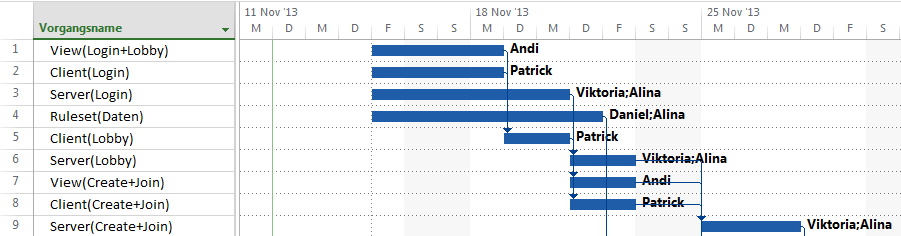
\includegraphics[width=1.2\textwidth]{Milestone1} \\ \\

\hspace*{-0.1\textwidth}Milestone 2: \\ \\
\hspace*{-0.1\textwidth}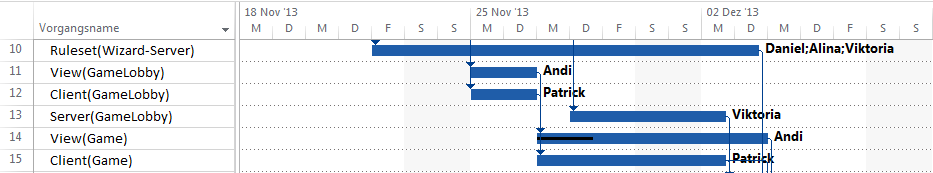
\includegraphics[width=1.2\textwidth]{Milestone2} \\ \\

\hspace*{-0.1\textwidth}Milestone 3: \\ \\
\hspace*{-0.1\textwidth}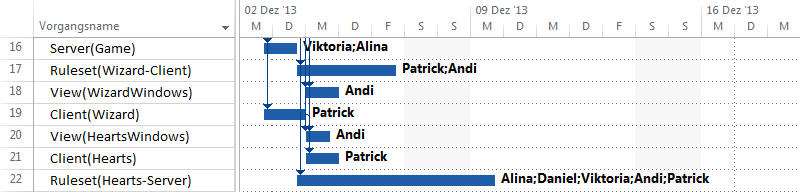
\includegraphics[width=1.2\textwidth]{Milestone3} \\ \\

\hspace*{-0.1\textwidth}Finale Version: \\ \\
\hspace*{-0.1\textwidth}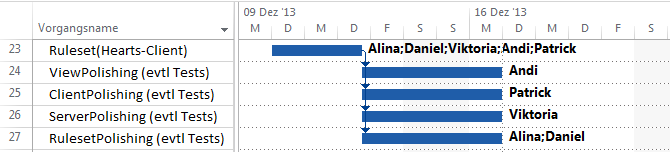
\includegraphics[width=1.2\textwidth]{Milestone4} \\ \\
% Index
\newpage
\phantomsection
\addcontentsline{toc}{part}{Index}
\printindex

\end{document}
